\documentclass[11pt,oneside]{uhthesis}
\usepackage{subfigure}

\usepackage[ruled,lined,linesnumbered,titlenumbered,algochapter,spanish,onelanguage]{algorithm2e}
\SetKwIF{Si}{SinoSi}{Sino}{si}{entonces}{si no}{si no si}{fin si}
\SetKw{OtroCaso}{otro caso}
\SetKwBlock{Caso}{caso}{fin caso}
\SetKwFor{Para}{para}{hacer}{fin para}
\SetKwFor{Mientras}{mientras}{hacer}{fin mientras}
\SetKw{Retorna}{retorna}

\usepackage{amsmath}
\usepackage{amssymb}
\usepackage{amsbsy}
\usepackage{caption,booktabs}
\captionsetup{ justification = centering }
%\usepackage{mathpazo}
\usepackage{float}
\setlength{\marginparwidth}{2cm}
\usepackage{todonotes}
\usepackage{listings}
\usepackage{xcolor}
\usepackage{multicol}
\usepackage{graphicx}

\usepackage[most]{tcolorbox}


\floatstyle{plaintop}
\restylefloat{table}
\addbibresource{Bibliography.bib}
% \setlength{\parskip}{\baselineskip}%
\renewcommand{\tablename}{Tabla}
\renewcommand{\listalgorithmcfname}{Índice de Algoritmos}
%\dontprintsemicolon
\SetAlgoNoEnd

\definecolor{codegreen}{rgb}{0,0.6,0}
\definecolor{codegray}{rgb}{0.5,0.5,0.5}
\definecolor{codepurple}{rgb}{0.58,0,0.82}
\definecolor{backcolour}{rgb}{0.95,0.95,0.92}

\lstdefinestyle{mystyle}{
    backgroundcolor=\color{backcolour},   
    commentstyle=\color{codegreen},
    keywordstyle=\color{purple},
    numberstyle=\tiny\color{codegray},
    stringstyle=\color{codepurple},
    basicstyle=\ttfamily\footnotesize,
    breakatwhitespace=false,         
    breaklines=true,                 
    captionpos=b,                    
    keepspaces=true,                 
    numbers=left,                    
    numbersep=5pt,                  
    showspaces=false,                
    showstringspaces=false,
    showtabs=false,                  
    tabsize=4
}

\lstset{style=mystyle}

\title{\texttt{PLAN-GRAIL}: mejorando la correctitud sintáctica y semántica de agentes basados en \textit{LLMs} para modelación de problemas de planificación}
\author{\\\vspace{0.25cm}Ariel González Gómez}
\advisor{\\\vspace{0.25cm}Dr. Alejandro Piad Morfiss\\\vspace{0.2cm}Dr. Yudivián Almeida Cruz}
\degree{Licenciado en Ciencia de la Computación}
\faculty{Facultad de Matemática y Computación}
\date{La Habana\\junio de 2025\\\vspace{0.25cm}\href{https://github.com/arielgg46/Thesis}{github.com/arielgg46/Thesis}}
\logo{Graphics/UH}
\faclogo{Graphics/matcom}
\makenomenclature

\renewcommand{\vec}[1]{\boldsymbol{#1}}
\newcommand{\diff}[1]{\ensuremath{\mathrm{d}#1}}
\newcommand{\me}[1]{\mathrm{e}^{#1}}
\newcommand{\pf}{\mathfrak{p}}
\newcommand{\qf}{\mathfrak{q}}
%\newcommand{\kf}{\mathfrak{k}}
\newcommand{\kt}{\mathtt{k}}
\newcommand{\mf}{\mathfrak{m}}
\newcommand{\hf}{\mathfrak{h}}
\newcommand{\fac}{\mathrm{fac}}
\newcommand{\maxx}[1]{\max\left\{ #1 \right\} }
\newcommand{\minn}[1]{\min\left\{ #1 \right\} }
\newcommand{\lldpcf}{1.25}
\newcommand{\nnorm}[1]{\left\lvert #1 \right\rvert }
\renewcommand{\lstlistingname}{Ejemplo de código}
\renewcommand{\lstlistlistingname}{Ejemplos de código}

\begin{document}

\frontmatter
\maketitle

\begin{dedication}
\textit{``It's the questions we can't answer that teach us the most.}

\textit{They teach us how to think.}

\textit{If you give a man an answer, all he gains is a little fact.} 

\textit{But give him a question and he'll look for his own answers.''}

\textit{\textbf{― Patrick Rothfuss, The Wise Man's Fear}}
\end{dedication}
\begin{acknowledgements}
Quiero agradecer, en primer y destacado lugar, a toda mi familia, por ser mi apoyo vital, emocional y formador. Solo lo que me han otorgado, con enorme amor y sacrificios, ha hecho posible que llegue tan lejos en la vida.

A mi madre, que fue mi primera tutora, que veló mis primeros pasos en la programación, adentrándome en este mundo tan hermoso, y que me ha acompañado de la mano todo el camino. Ponerla orgullosa de mí motiva mi búsqueda de la perfección, en todo lo que hago.

A mi padre, que me enseñó a ser fuerte, a mantenerme positivo en todo momento y, en las situaciones más difíciles, aguantar y seguir avanzando. De él aprendí que cualquier cosa que me propongo, lo hago bien o no lo hago.

A mi hermana, mi cotutora, mi modelo a seguir. Por siempre desempeñar con excelencia el papel de la hermana mayor, por ser mi bastón ético y moral, y por hacerme reir cuando lo necesitaba.

A mis abuelos, por cuidarme, sostenerme, y mimarme como solo ellos saben hacer.

A mis amigos cercanos, que he tenido la suerte de tener muchos y muy buenos. Si los listo, siempre habrá aquel que se quedó fuera y se pondrá celoso, así que ya me aseguraré de agradecerles en persona. Por estar ahí cuando los necesité, por ser mi fuente inacabable de experiencias, motivación y el equilibrio personal durante esta y otras etapas, y bueno, por las risas.

A mis tutores, por confiar en mi trabajo, por su guía experta, paciencia, atención y apoyo constante a lo largo de este proceso.

A mis profesores de todas las enseñanzas. Ellos construyeron la base académica y docente que me llevó a este punto. Un agradecimiento particular a Lupe, que motivó mi amor por la matemática, y la enseñanza.

Finalmente, a las instituciones y fuentes de financiamiento que hicieron posible el acceso a recursos y herramientas necesarios para llevar adelante esta investigación. A los autores de los trabajos científicos que la anteceden y sobre los que se basa.

Muchísimas gracias a todos.

\end{acknowledgements}
\begin{opinion}
Como tutor del trabajo de diploma titulado ``\texttt{PLAN-GRAIL}: mejorando la correctitud sintáctica y semántica de agentes basados en \textit{LLMs} para modelación de problemas de planificación'', realizado por Ariel González Gómez, expreso mi valoración sobre la importancia, originalidad y calidad de la investigación desarrollada.

El tema abordado en esta tesis se sitúa en el centro de uno de los retos más relevantes de la inteligencia artificial contemporánea: el razonamiento de los Modelos de Lenguaje de Gran Escala (\textit{LLMs}) mediante su integración con herramientas externas. En particular, la generación automática de modelos simbólicos (\textit{PDDL}) a partir de descripciones en lenguaje natural es un problema de alto impacto, pues constituye un cuello de botella para la adopción práctica de planificadores clásicos en numerosos contextos reales. Sin embargo, la integración de \textit{LLMs} con planificadores simbólicos presenta desafíos notables, ya que los modelos tienden a ``alucinar'' características del entorno, sin comprensión del problema, lo que provoca errores sintácticos y semánticos difíciles de controlar. Por ello, la necesidad de garantizar la correctitud formal de las salidas es crítica para la confiabilidad de los sistemas híbridos simbólico-conectivistas.

La tesis de Ariel representa un avance significativo sobre el estado del arte en este campo. El trabajo propone una arquitectura modular y extensible para agentes modeladores basados en \textit{LLMs}, que resuelve de manera definitiva el problema de la correctitud sintáctica en la generación de modelos \textit{PDDL}. Esto se logra mediante la integración de técnicas de \textit{Grammar-Constrained Decoding (GCD)} y la generación automática de gramáticas especializadas para cada instancia de problema, lo que asegura no solo la validez sintáctica (eliminando completamente los errores de \textit{parsing}), sino también una mejora sustancial en la correctitud semántica de las soluciones generadas—con incrementos de hasta 24.3 \% respecto a los mejores \textit{baselines} reproducidos y un desempeño de 100 \% en validez sintáctica, 87.1 \% en solubilidad y 81.4 \% en correctitud. Más aún, la integración de mecanismos de reintentos, guiados por \textit{feedback} construido automáticamente y autorreflexión de los modelos, permitió elevar estas métricas a 100\,\%, 98.57\,\% y 84.29\,\%, respectivamente. Finalmente, agregando el componente experiencial, consistente en la recuperación por \textit{RAG} de ejemplos similares de soluciones obtenidas durante el entrenamiento, así como la inclusión en el \textit{prompt} de \textit{insights} de modelación, se consiguió la solubilidad del 100\,\% de los modelos, y la correctitud del 87.14\,\%.

Entre las innovaciones principales de la tesis destacan:

\begin{itemize}
\item La generación automática de gramáticas con contenido semántico específico para cada instancia de problema, restringiendo la generación a predicados, aridad y tipos válidos según el dominio y los objetos extraídos.

\item La incorporación de un agente experiencial capaz de recolectar y utilizar \textit{insights} y reflexiones a partir de problemas similares, permitiendo un proceso de \textit{Transfer Learning} en un entorno socrático, sin necesidad de \textit{Fine-Tuning} ni modificación de los pesos del modelo.

\item El uso combinado de razonamiento estructurado en fases, \textit{feedback} automático, aprendizaje experiencial y \textit{Retrieval-Augmented Generation (RAG)} para enriquecer el contexto y guiar la generación hacia soluciones más fieles y robustas.
\end{itemize}

Los resultados obtenidos no solo superan en un orden de magnitud la correctitud de las soluciones generadas respecto a los métodos existentes, sino que establecen un nuevo estándar de referencia en la generación automática de modelos simbólicos asistida por \textit{LLMs}. La arquitectura, los métodos y las métricas de evaluación propuestos son reproducibles y de gran valor para la comunidad, con resultados que son plenamente publicables en el primer nivel científico internacional.

Cabe resaltar que todo el mérito de estos logros corresponde a Ariel González Gómez, quien trabajó con absoluta independencia durante todas las etapas del proceso investigativo: desde la revisión crítica del estado del arte, el diseño conceptual, la implementación técnica y experimental, hasta el análisis y discusión de los resultados. Ariel demostró iniciativa, rigor, creatividad y una capacidad sobresaliente para abordar problemas abiertos y proponer soluciones originales y efectivas.

Por todo lo anterior, considero que esta tesis constituye una contribución destacada al avance del campo y recomiendo su aprobación con la máxima calificación. Felicito a Ariel por su desempeño académico y científico ejemplar.

\vspace{0.5cm}

\begin{flushright}
	\underline{\hspace{6.5cm}}\\
	Dr. Alejandro Piad Morfiss
	
	Facultad de Matemática y Computación
	
	Universidad de la Habana
	
	Junio, 2025
\end{flushright}

\end{opinion}
\begin{resumen}
El modelado simbólico de tareas de planificación representa uno de los principales cuellos de botella para la adopción de planificadores clásicos en contextos reales. Si bien el paradigma \textit{LLM-as-Planner} ha ganado atención reciente, enfrenta serias limitaciones en verificabilidad y optimalidad. Como alternativa, esta tesis se inscribe en el enfoque \textit{LLM-as-Modeler}, en el que agentes basados en \textit{Large Language Models (LLMs)} generan automáticamente modelos \textit{PDDL (Planning Domain Definition Language)} de los problemas a partir de sus descripciones en lenguaje natural. Se propone un agente modelador modular y extensible, diseñado para mejorar la validez sintáctica, solubilidad y correctitud semántica de los modelos generados. La arquitectura combina múltiples técnicas complementarias: razonamiento estructurado en fases, generación restringida por gramática mediante \textit{Grammar-Constrained Decoding (GCD)}, \textit{feedback} automático y reflexión sobre fallos, aprendizaje experiencial con extracción y refinamiento de soluciones e \textit{insights}, y \textit{Few-Shot Prompting} enriquecido con \textit{Retrieval-Augmented Generation (RAG)}. 

La evaluación empírica se realizó sobre subconjuntos estratificados del \textit{benchmark} \textit{Planetarium}, comparando \textit{baselines} relevantes del trabajo \textit{LLM+P} y variantes del agente propuesto. Los resultados muestran mejoras significativas en todas las métricas clave, destacando la eliminación completa de errores sintácticos con \textit{GCD} mediante gramáticas especializadas y un aumento de hasta \textbf{24.3\,\%} en correctitud semántica respecto al mejor \textit{baseline} reproducido, cerrando \textbf{56.7\,\%} de su margen de mejora. La inclusión conjunta de razonamiento estructurado, extracción de objetos y \textit{GCD} permitió un desempeño de \textbf{100\,\%} en validez sintáctica, \textbf{87.1\,\%} en solubilidad y \textbf{81.4\,\%} en correctitud. Al incorporar mecanismos de reflexión y retroalimentación automática, se corrigieron errores residuales, elevando la solubilidad a \textbf{98.57\,\%} y la correctitud a \textbf{84.29\,\%}. Finalmente, la combinación sinérgica de reintentos con reflexión, recuperación de ejemplos previos e \textit{insights} construidos manualmente permitió elevar las tasas anteriores a \textbf{100\,\%} y \textbf{87.14\,\%}, respectivamente.

Este trabajo aporta una arquitectura funcional, un marco de evaluación reproducible y evidencia empírica de que los \textit{LLMs}, adecuadamente guiados y entrenados, pueden ser agentes modeladores efectivos. La propuesta abre nuevas perspectivas para el diseño de sistemas híbridos simbólico-conectivistas en planificación automática, con menor dependencia de intervención humana experta.
\end{resumen}

\begin{abstract}
Symbolic modeling of planning tasks remains one of the main bottlenecks for the practical adoption of classical planners in real-world contexts. While the \textit{LLM-as-Planner} paradigm has recently gained attention, it faces serious limitations in verifiability and optimality. As an alternative, this thesis adopts the \textit{LLM-as-Modeler} approach, in which agents based on \textit{Large Language Models (LLMs)} automatically generate \textit{PDDL (Planning Domain Definition Language)} models of planning problems from their natural language descriptions. A modular and extensible modeling agent is proposed, designed to improve the parseability, solvability, and semantic correctness of the generated models. The architecture combines multiple complementary techniques: structured multi-phase reasoning, \textit{Grammar-Constrained Decoding (GCD)}, automatic feedback and failure-driven reflection, experiential learning through solution and \textit{insight} extraction and refinement, and \textit{Few-Shot Prompting} enriched with \textit{Retrieval-Augmented Generation (RAG)}.

Empirical evaluation was conducted on stratified subsets of the \textit{Planetarium} benchmark, comparing relevant \textit{LLM+P} baselines and several variants of the proposed agent. Results show significant improvements across all key metrics, including the complete elimination of syntactic errors via \textit{GCD} with specialized grammars, and an increase of up to \textbf{24.3\,\%} in semantic correctness over the best reproduced \textit{baseline}, closing \textbf{56.7\,\%} of its performance gap. The combined inclusion of structured reasoning, object extraction, and \textit{GCD} enabled a performance of \textbf{100\,\%} parseability, \textbf{87.1\,\%} solvability, and \textbf{81.4\,\%} correctness. By incorporating mechanisms for reflection and automatic feedback, residual errors were corrected, raising solvability to \textbf{98.57\,\%} and correctness to \textbf{84.29\,\%}. Finally, the synergistic combination of retries with reflection, retrieval of prior examples, and manually constructed \textit{insights} further increased these rates to \textbf{100\,\%} and \textbf{87.14\,\%}, respectively.

This work contributes a functional architecture, a reproducible evaluation framework, and empirical evidence that properly guided and trained \textit{LLMs} can serve as effective modeling agents. The proposed approach opens new perspectives for the design of hybrid neuro-symbolic systems in automated planning, with reduced reliance on expert human intervention.
\end{abstract}
\tableofcontents
\listoffigures
% \listoftables
% \listofalgorithms
\lstlistoflistings

\mainmatter

\chapter*{Introducción}\label{chapter:introduction}
\addcontentsline{toc}{chapter}{Introducción}

En las últimas décadas, los problemas de planificación han adquirido creciente relevancia tanto en el ámbito académico como industrial, al ofrecer soluciones formales para tareas que implican asignación de recursos, secuenciación de actividades o coordinación de agentes autónomos \parencite{li2024lasp, ghallab2004automated}. Desde la robótica de servicio hasta la gestión de flotas de vehículos, muchas de estas tareas pueden formularse como problemas de planificación \parencite{li2024lasp, karpas2020automated, marrella2019automated}, resueltos mediante algoritmos clásicos, como planificadores heurísticos sobre lenguajes formales como \textit{Planning Domain Definition Language (PDDL)} \parencite{aeronautiques1998pddl}. 

Pese a sus grandes beneficios, el uso de los algoritmos clásicos está limitado por la fase de modelado del problema. Sin embargo, han surgido recientemente enfoques basados en Modelos de Lenguaje de Gran Escala (\textit{Large Language Models - LLMs)}, que buscan reducir la carga del modelado simbólico o incluso reemplazar al planificador. El paradigma \textit{LLM-as-Planner} propone generar directamente secuencias de acciones desde lenguaje natural, pero presenta limitaciones importantes en factibilidad, verificabilidad y optimalidad \parencite{aghzal2025survey}. 

Como alternativa, el enfoque \textit{LLM-as-Modeler} traslada el esfuerzo al modelado automático en \textit{PDDL}, delegando la planificación a algoritmos simbólicos consolidados. Esta estrategia combina capacidades lingüísticas con garantías formales, pero aún enfrenta obstáculos relevantes: errores sintácticos, inconsistencias semánticas y fuerte dependencia de supervisión humana. Para abordar estas limitaciones, se propone utilizar estrategias complementarias como la limitación de la salida del \textit{LLM} a la sintaxis de \textit{PDDL} y su gramática correspondiente con  \textit{Grammar‑Constrained Decoding (GCD)} \parencite{geng2023grammar}, inclusión de fases previas de razonamiento estructurado y extracción de objetos, técnicas de \textit{Retrieval-Augmented Generation (RAG)} \parencite{gao2023retrieval} y aprendizaje experiencial como en el antecedente \textit{ExpeL} \parencite{zhao2024expel}, y recursos de entrenamiento y evaluación sistemática del \textit{benchmark} \textit{Planetarium} \parencite{zuo2024planetarium}. Esta tesis se inscribe en este panorama, y propone contribuir a la mejora del modelado automático con \textit{LLMs}, sin comprometer su escalabilidad ni requerir intervenciones costosas. El nombre en inglés del sistema propuesto es el acrónimo \texttt{PLAN-GRAIL}: \textit{\underline{P}lanning with \underline{L}LM-based \underline{A}gents via \underline{N}euro-symbolic modeling with \underline{G}rammar-Constrained Decoding, \underline{R}easoning and \underline{A}ctive \underline{I}n-Context \underline{L}earning}.

\section*{Motivación y Antecedentes}

Desde los años 70, la comunidad de planificación ha desarrollado lenguajes formales como \textit{STRIPS} y \textit{PDDL} \parencite{fikes1971strips, aeronautiques1998pddl}, junto con planificadores simbólicos clásicos como \textit{Fast Downward} o \textit{LAMA} \parencite{helmert2006fast, richter2011lama}, que permiten resolver tareas complejas en entornos estructurados. Sin embargo, su despliegue práctico sigue limitado por el alto costo del modelado formal: construir manualmente dominios y problemas en \textit{PDDL} requiere experticia técnica, atención a la sintaxis y comprensión profunda del dominio, lo cual restringe su adopción en contextos reales.

La aparición de los \textit{LLMs}, como \textit{GPT-3} \parencite{brown2020language}, ha motivado nuevas estrategias para aliviar esta carga. Inicialmente se exploró el paradigma \textit{LLM-as-Planner}, donde el modelo genera directamente un plan desde lenguaje natural \parencite{aghzal2025survey, wei2025plangenllms}, pero esta línea enfrenta dificultades severas en factibilidad, optimalidad y verificabilidad de los planes generados \parencite{kambhampati2024position}.

Como alternativa, surge el enfoque \textit{LLM-as-Modeler}, en el cual el \textit{LLM} traduce la descripción textual a un modelo en \textit{PDDL} del problema, delegando la búsqueda del plan a los motores clásicos \parencite{tantakoun2025llms, liu2023llm+}. Este paradigma permite aprovechar las fortalezas combinadas del procesamiento lingüístico de los \textit{LLMs} y las garantías formales de los planificadores simbólicos, pero sigue enfrentando desafíos importantes: errores sintácticos, inconsistencias semánticas y dependencia de intervención humana.

Múltiples trabajos han propuesto soluciones complementarias. Algunos exploran mecanismos intermedios o ciclos de verificación \parencite{agarwal2024tic}, mientras que otros adoptan \textit{Fine-Tuning} sobre corpus especializados \parencite{zeng2023agenttuning, zuo2024planetarium}. No obstante, estas estrategias suelen ser costosas, difíciles de escalar y dependientes de infraestructura técnica avanzada y labor humana experta, lo cual motiva la búsqueda de alternativas más ligeras y generalizables, como el \textit{In-Context Learning} \parencite{dong2022survey}.

A pesar de los avances recientes, la problemática es evidente: la generación automática de problemas \textit{PDDL} mediante \textit{LLMs} sigue enfrentando retos fundamentales, en especial en lo que respecta a la fidelidad semántica y la validez formal de los modelos producidos \parencite{zuo2024planetarium}. Aunque herramientas como \textit{Planetarium} han facilitado su evaluación sistemática, los errores persisten: el uso de predicados no declarados o tipos incorrectos, paréntesis desbalanceados, parámetros duplicados, etc., constituyen errores sintácticos del archivo \textit{PDDL} generado. Semánticamente, el uso de predicados de coexistencia contradictoria, o sin conexión con el estado inicial o los objetivos, impiden la resolución correcta del problema. Estos errores reflejan no solo dificultades con la sintaxis del lenguaje de planificación, sino también una comprensión limitada del dominio y de los requisitos lógicos implícitos en la planificación simbólica. Además, las soluciones a estos mismos problemas propuestas hasta la fecha presentan limitaciones y desventajas propias, fundamentalmente la fuerte dependencia de conocimiento experto e intervención humana laboriosa, y los altos costos computacionales.

La motivación y justificación directa de esta tesis radica en una observación concreta: aunque los algoritmos clásicos de planificación automática están disponibles y son eficaces, su uso en la práctica sigue siendo escaso debido a la complejidad del modelado. Al mismo tiempo, los \textit{LLMs} ya están integrados en diversas herramientas de software, y su potencial para ayudar en tareas estructuradas es alto si se les orienta con estrategias adecuadas, para superar las limitaciones inherentes de estos modelos y de los enfoques actuales. Esta investigación busca precisamente avanzar en esa dirección.

La existencia de ciertos trabajos anteriores inspiran directamente el enfoque que toma esta tesis, y el uso de sus estrategias y técnicas se justifica por las limitaciones identificadas que podrían aliviar. Primero, la técnica de \textit{Grammar-Constrained Decoding (GCD)} permite restringir la salida del modelo a una gramática formal predefinida, asegurando la validez sintáctica\footnote{\textit{Parseability}, término en inglés que se refiere a la correctitud sintáctica, o la propiedad de ser analizable por un \textit{parser} del lenguaje formal definido, sin errores de sintaxis.} del \textit{PDDL} generado sin modificar los pesos del modelo \parencite{geng2023grammar}. Segundo, el enfoque experiencial propuesto en \textit{ExpeL} \parencite{zhao2024expel} demuestra que los modelos pueden adquirir conocimiento estructurado de planificación a partir de ejemplos resueltos, mediante ciclos de prueba y refinamiento, en un entrenamiento previo del agente. Tercero, el \textit{benchmark Planetarium} \parencite{zuo2024planetarium} provee un \textit{corpus} masivo de pares texto-\textit{PDDL} junto con métricas automáticas de validez sintáctica, solubilidad (posibilidad de encontrar un plan válido en el dominio que llegue del estado inicial al objetivo definidos en el modelo, usualmente por un planificador clásico) y equivalencia semántica (fidelidad del modelo a la descripción en lenguaje natural del problema), lo que permite tanto el entrenamiento experiencial como la evaluación sistemática de agentes modeladores.

Estos antecedentes evidencian el potencial de combinar restricciones gramaticales, aprendizaje experiencial e infraestructura de evaluación robusta para avanzar hacia agentes modeladores con \textit{LLMs} más eficaces, generalizables y prácticos. Esta tesis se inscribe en dicha dirección.

\section*{Problema científico y Ámbito del problema}

Actualmente, los agentes basados en \textit{LLMs} que a partir de descripciones en lenguaje natural generan sus representaciones en \textit{PDDL}, con una dependencia humana reducida, presentan dificultades para asegurar que los modelos generados sean válidos sintácticamente, solubles por un planificador clásico y semánticamente correctos o fieles a la intención expresada en el texto.

El objeto de estudio de esta investigación se enmarca en la modelación automática de problemas de planificación a partir de descripciones en lenguaje natural, utilizando agentes basados en \textit{LLMs}.

El campo de acción se circunscribe al diseño e implementación de agentes basados en \textit{LLMs}, para modelación de problemas de planificación, enfocado en la generación automática de archivos \textit{PDDL} en dominios de planificación bien definidos y deterministas. Se incluye, además, la evaluación empírica de los agentes a través del \textit{benchmark Planetarium} mediante métricas de validez sintáctica, solubilidad y fidelidad semántica.

\section*{Hipótesis}
El presente trabajo plantea una serie de hipótesis acerca del impacto de distintas técnicas y estrategias que buscan mejorar los resultados, en las métricas contempladas, de agentes basados en \textit{LLMs} para modelación de tareas de planificación:

\begin{itemize}
    \item[\textbf{H1.}] La división del proceso de modelado en fases estructuradas —extracción de objetos, razonamiento, especificación del estado inicial y metas, y generación del archivo \textit{PDDL}— mejora la correctitud de los modelos generados, al permitir un razonamiento más controlado, modular y verificable.
    \item[\textbf{H2.}] La aplicación de \textit{GCD}  permite una generación más confiable del código \textit{PDDL}, reduciendo significativamente o eliminando por completo la aparición de errores de sintaxis.
    \item[\textbf{H3.}] La introducción de reflexión sobre errores y una mínima retroalimentación humana o automática permite al agente corregir patrones de falla recurrentes, contribuyendo al aumento de la solubilidad y la correctitud del \textit{PDDL} generado.
    \item[\textbf{H4.}] La incorporación de \textit{RAG} para la selección de ejemplos relevantes y la extracción de \textit{insights} a partir de soluciones previas (tanto correctas como erróneas), representa una vía prometedora para mejorar la capacidad de los agentes basados en \textit{LLMs} para modelar tareas de planificación, al permitirles adaptarse a la semántica de nuevas tareas y fortalecer su conocimiento sobre el dominio específico y la modelación de problemas.
\end{itemize}

\section*{Objetivo General}

Diseñar, implementar y evaluar agentes basados en \textit{LLMs} con técnicas propuestas para mejorar la correctitud sintáctica y semántica de la generación de códigos \textit{PDDL} en modelación de tareas de planificación, y realizar un análisis comparativo de los agentes implementados para determinar los factores que influyen positivamente en métricas como validez sintáctica, solubilidad y correctitud.

\section*{Objetivos Específicos}

\begin{enumerate}
	\item Realizar un estudio del estado del arte de agentes basados en \textit{LLMs} para modelación de problemas de planificación.

	\item Presentar un marco teórico-conceptual para establecer las definiciones fundamentales relacionados con la planificación automática, y las técnicas y recursos a utilizar en la propuesta de solución.

	\item Diseñar un agente basado en \textit{LLM} y variantes del mismo con técnicas propuestas para mejorar la correctitud sintáctica y semántica de la generación de códigos \textit{PDDL} en modelación de tareas de planificación, así como sus fases de entrenamiento, evaluación y análisis comparativo de los agentes propuestos y \textit{baselines} extraídos de los antecedentes descritos en la literatura. 

	\item Implementar los \textit{baselines}, el agente diseñado y sus variantes, para el posterior análisis de cómo afectan las distintas técnicas e ideas al rendimiento según métricas de validez sintáctica, solubilidad y correctitud. Además, implementar los \textit{pipelines} de generación de los subconjuntos de problemas para entrenamiento y evaluación de los agentes, así como los algoritmos que describen estos propios procesos.

	\item Evaluar las distintas variantes del agente en un \textit{benchmark} que permita analizar el rendimiento de agentes modeladores de problemas de planificación, según las métricas propuestas.

	\item Realizar un estudio estadístico y de ablación de los resultados de la evaluación, para identificar concretamente las posibles influencias que tienen las técnicas y métodos usados en las métricas analizadas.
	
\end{enumerate}

\section*{Propuesta de solución}

La presente investigación propone el desarrollo de agentes modeladores de problemas de planificación basados en \textit{LLMs}, cuya función principal sea la generación automática de archivos de problema \textit{PDDL} a partir de descripciones en lenguaje natural. El \textit{PDDL} generado se utiliza como entrada a un sistema planificador clásico (\textit{Fast Downward}) para generar un plan eficiente que resuelve el problema. Este agente opera en modalidad \textit{Open-Loop}\footnote{Un agente \textit{Open-Loop} genera un plan completo y estático antes de ejecutar cualquier acción, asumiendo un entorno determinista y sin incorporar retroalimentación durante la ejecución. Este enfoque contrasta con los sistemas \textit{Closed-Loop}, que ajustan el plan dinámicamente ante fallos o cambios en el entorno \parencite{wei2025plangenllms}.}, asumiendo un entorno determinista y sin retroalimentación del entorno, y es evaluado bajo el marco riguroso del \textit{benchmark Planetarium}, el cual permite medir automáticamente la validez sintáctica, solubilidad y correctitud semántica de los modelos generados. La entrada de los agentes es de base la descripción del dominio del problema, el archivo \textit{PDDL} del dominio, y la descripción en lenguaje natural del problema.

Para asegurar la validez sintáctica del código \textit{PDDL} generado por el agente modelador, se integra \textit{GCD} utilizando como \textit{baseline} una gramática \textit{GBNF} (\textit{Georgi Gerganov's Machine Learning (GGML) Backus--Naur form (BNF)}) \parencite{ggml2023gbnf}, derivada de la sintaxis general del subconjunto \textit{STRIPS} y \textit{:typing} de \textit{PDDL}. Se propone también el uso de gramáticas generadas automática y específicamente para el dominio y el problema a partir de una fase previa de extracción de objetos tipados, para limitar la generación de predicados a estos objetos, con aridad y tipado de argumentos correctos. Esta técnica se aplica tanto a la generación final del archivo \textit{PDDL} como a la fase intermedia de extracción de objetos.

Con inspiración en el enfoque experiencial del trabajo de \textit{ExpeL} bajo el paradigma \textit{LLM-as-Planner}, se propone su adaptación al paradigma \textit{LLM-as-Modeler}. Durante una fase de entrenamiento sobre un subconjunto estratificado del \textit{dataset Planetarium}, el agente recopila un conjunto de soluciones correctas e incorrectas. A partir de estas, se realiza una extracción sistemática de \textit{insights} (conocimiento condensado), orientada a mejorar el conocimiento general de modelación de problemas de planificación, así como a capturar conocimiento específico por dominio (por ejemplo, sobre el uso de predicados, limitaciones o reglas del dominio, o sus patrones típicos). Esta fase es reforzada en su mayoría con mecanismos de refinamiento mediante \textit{In-Context Reinforcement Learning}, y reflexión sobre fallos con \textit{feedback} (retroalimentación) construido automáticamente o por intervención humana mínima. Estos conocimientos se integran en el comportamiento del agente a través de \textit{In-Context Learning}.

Para mejorar la fidelidad semántica y la coherencia de las salidas, se emplea \textit{Few-Shot Prompting} enriquecido con \textit{RAG}, utilizando \textit{embeddings} de lenguaje natural de las descripciones textuales, para seleccionar ejemplos previos relevantes del \textit{corpus} de soluciones correctas construido durante la fase de entrenamiento. Un conjunto de \textit{insights} evoluciona mediante la actualización automática, por un \textit{LLM}, de los pesos y descripciones de los \textit{insights} mediante operaciones bien definidas. Esto permite una adaptación progresiva del agente basada en su experiencia acumulada durante el entrenamiento, con mínima intervención experta.

Para evaluar el impacto de cada componente del agente propuesto, se lleva a cabo un estudio comparativo incremental (en cuanto a las variantes evaluadas) sobre el \textit{dataset Planetarium}. Se diseñan distintas variantes del agente, activando o desactivando módulos específicos (como \textit{GCD}, Razonamiento estructurado o Extracción de objetos). Además se implementan \textit{baselines} contra los que comparar las variantes propuestas, como los agentes principales del trabajo de \textit{LLM+P} \parencite{liu2023llm+}: \textbf{LLM-as-P\textsuperscript{-}} (agente planificador \textit{Zero-shot}), \textbf{LLM-as-P\textsuperscript{+}} (agente planificador \textit{One-shot} con ejemplo fijo), \textbf{LLM+P\textsuperscript{-}} (agente modelador \textit{Zero-shot}) y \textbf{LLM+P\textsuperscript{+}} (agente modelador \textit{One-shot} con ejemplo fijo). Se miden los resultados de todos los agentes en subconjuntos estratificados del \textit{dataset}. Esto permite analizar la contribución relativa de cada técnica a la mejora de las métricas clave, así como la evolución de la calidad de las salidas del agente conforme se integran mecanismos más sofisticados de comprensión, generación y adaptación.

\section*{Estructura de la tesis}

La presente tesis se estructura en capítulos organizados de forma progresiva para guiar al lector desde el contexto del problema y los fundamentos conceptuales, hasta el diseño, implementación, evaluación y análisis de la solución propuesta:

\begin{itemize}
    \item \textbf{Introducción} \\
    Se presenta el contexto histórico-social donde se desarrolla la investigación, los antecedentes del problema, la problemática, la motivación y justificación, el diseño teórico, las hipótesis, los objetivos, la propuesta de solución y la estructura del trabajo.

    \item \textbf{Capítulo 1: Estado del Arte y Marco Teórico-Conceptual} \\
    Se realiza una revisión crítica de trabajos previos relevantes, incluyendo estudios sobre generación automática de \textit{PDDL} con \textit{LLMs}, agentes planificadores, agentes modeladores, enfoques recientes, etc. Se identifican las limitaciones existentes y se posiciona la contribución de esta tesis dentro del campo. Se abordan los conceptos fundamentales relacionados con la planificación automática, el lenguaje \textit{PDDL}, los modelos de lenguaje de gran escala (\textit{LLMs}), las técnicas de generación estructurada como \textit{GCD}, y los enfoques de razonamiento, aprendizaje experiencial, autorreflexión, \textit{In-Context Learning} reforzado con \textit{RAG}, etc. También se describe el \textit{benchmark Planetarium} y su sistema de evaluación.
    
    \item \textbf{Capítulo 2: Propuesta de Solución} \\
    Se describe el diseño del agente planificador propuesto, sus distintas fases (razonamiento, extracción de objetos, generación de \textit{PDDL}) y el uso de \textit{GCD} en diversas etapas. Se detalla el procedimiento de entrenamiento en acumulación de experiencias y extracción de \textit{insights}, el diseño de los \textit{prompts} y las gramáticas.
    
    \item \textbf{Capítulo 3: Implementación de la propuesta} \\
    Se explican las herramientas utilizadas, la arquitectura del sistema, y las decisiones y detalles de implementación.
    
    \item \textbf{Capítulo 4: Evaluación} \\
    Se presentan los experimentos realizados sobre el \textit{benchmark Planetarium}, comparando variantes del agente y evaluando su rendimiento según validez sintáctica, solubilidad y correctitud. Se analiza la influencia de cada componente de la mejora propuesta sobre estas métricas. Se justifican los experimentos propuestos respecto al análisis de cumplimiento de las hipótesis, en el contexto con limitaciones a las que las evaluaciones están sujetas.
    
    \item \textbf{Conclusiones} \\
    Se sintetizan los resultados obtenidos, se evalúa el cumplimiento de los objetivos y la validez de las hipótesis bajo las limitaciones observadas.
    
   \item \textbf{Recomendaciones y Trabajo Futuro} \\
    Se proponen múltiples líneas de trabajo futuras para mejorar y extender la propuesta, basadas en sus limitaciones e ideas de alto potencial no contempladas en esta investigación.

    \item \textbf{Bibliografía} \\
    Se presenta toda la bibliografía consultada para la realización de esta tesis, así como las referencias bibliográficas a literatura citada en este documento.
\end{itemize}
\chapter{Estado del Arte y Marco Teórico-Conceptual}\label{chapter:state-of-the-art}

\section{Fundamentos de la Planificación Automática}

La \textit{Planificación Automática} (\textit{Automated Planning}, AP) es una subdisciplina de la inteligencia artificial centrada en la síntesis de secuencias de acciones para alcanzar un objetivo a partir de un estado inicial, sujeto a las restricciones impuestas por el entorno o dominio \parencite{tantakoun2025llms}. Su variante más reconocida es el \textit{problema clásico de planificación} (\textit{Classical Planning Problem}), que se formula bajo un conjunto de supuestos idealizados: el entorno es discreto, determinista, estático, completamente observable y monolítico (de un solo agente) \parencite{peter2021modern}. Este tipo de entorno permite diseñar agentes planificadores \textit{Open-Loop}, que ejecutan un plan sin requerir retroalimentación sensorial durante su ejecución.

Formalmente, un problema clásico de planificación puede definirse como una tupla:
\[
\mathcal{M} = \langle \mathcal{S}, s^{\mathcal{I}}, \mathcal{G}, \mathcal{A}, \mathcal{T} \rangle
\]
donde:
\begin{itemize}
    \item $\mathcal{S}$ es un conjunto finito y discreto de estados del mundo, definidos por una base de hechos atómicos sobre variables proposicionales.
    \item $s^{\mathcal{I}} \in \mathcal{S}$ representa el estado inicial del mundo.
    \item $\mathcal{G} \subseteq \mathcal{S}$ es el conjunto de estados objetivo que satisfacen las condiciones de meta.
    \item $\mathcal{A}$ es un conjunto finito de acciones simbólicas.
    \item $\mathcal{T}: \mathcal{S} \times \mathcal{A} \rightarrow \mathcal{S}$ es la función de transición que modela los efectos de aplicar una acción sobre un estado.
\end{itemize}

Una solución al problema es un \textit{plan} $\varphi = \langle a_1, a_2, \dots, a_n \rangle$, tal que las precondiciones de $a_1$ se satisfacen en $s^{\mathcal{I}}$, y la aplicación sucesiva de cada $a_i$ mediante $\mathcal{T}$ conduce a un estado que satisface los objetivos en $\mathcal{G}$ \parencite{tantakoun2025llms}.

\subsection{De \textit{STRIPS} a \textit{PDDL}}

La planificación como área formal emergió a partir de estudios de \textit{state-space search}, resolución de teoremas y teoría de control. Un sistema pionero fue \textit{STRIPS} (\textit{Stanford Research Institute Problem Solver}), desarrollado por Fikes y Nilsson como planificador para el robot \textit{Shakey} \parencite{peter2021modern}. Su estructura general se inspiró en el \textit{General Problem Solver} (\textit{GPS}) de Newell y Simon, que usaba análisis medios–fines como estrategia de búsqueda.

\textit{STRIPS} introdujo un lenguaje formal para describir acciones en términos de precondiciones y efectos (adición o eliminación de predicados), y su gramática básica es equivalente a la semántica conjuntista del modelo clásico \parencite{ghallab2004automated}. A lo largo del tiempo, este lenguaje fue extendido a \textit{ADL} (\textit{Action Description Language}) \parencite{pednault1987formulating}, incorporando cuantificadores, efectos condicionales y disyunciones. Finalmente, como descendiente natural, surgió \textit{PDDL} (\textit{Planning Domain Definition Language}) como estándar de representación para la \textit{International Planning Competition} (\textit{IPC}) desde 1998 \parencite{aeronautiques1998pddl}.

\textit{PDDL} está diseñado para describir tanto dominios clásicos como no clásicos, y permite extensiones que modelan observabilidad parcial, entornos estocásticos, múltiples agentes, concurrencia, planificación continua o a largo plazo. Estas dimensiones definen una taxonomía de variantes del problema clásico, dando lugar a planificadores \textit{Closed-Loop} cuando es necesaria la interacción en tiempo real con un entorno dinámico o parcialmente observable.

\subsection{Estructura de \textit{PDDL} y fragmento \textit{STRIPS + :typing}}

\textit{PDDL} organiza una tarea de planificación en dos archivos: el archivo de dominio $\mathbb{DF}$ y el archivo de problema $\mathbb{PF}$ \parencite{tantakoun2025llms}. El dominio define las constantes lógicas de la tarea, como predicados y acciones. Cada acción $a \in \mathcal{A}$ está definida por sus parámetros $\mathrm{Par}(a)$ (y sus tipos), sus precondiciones $\mathrm{Pre}(a)$ y sus efectos $\mathrm{Eff}(a)$, que determinan cómo se modifica el estado mediante la función $\mathcal{T}$.

El archivo de problema incluye los objetos concretos de la instancia, el estado inicial $s^{\mathcal{I}}$ y las metas $\mathcal{G}$. Gracias a su sintaxis clara y declarativa, \textit{PDDL} es fácilmente interpretable por modelos de lenguaje, que son capaces de mapear descripciones textuales a código \textit{PDDL} debido a su frecuente aparición en \textit{corpus} de entrenamiento modernos \parencite{tantakoun2025llms}.

Este trabajo se enfoca en un subconjunto del lenguaje, correspondiente al fragmento \textit{STRIPS}, junto con la extensión \texttt{:typing}. El fragmento \textit{STRIPS} restringe las acciones a precondiciones positivas y efectos que consisten únicamente en la adición o eliminación de predicados. La extensión \texttt{:typing} permite declarar jerarquías de tipos para los objetos, así como restricciones de tipado en los parámetros de acciones, facilitando la generalización y validación de modelos. Esta decisión técnica responde a las restricciones del benchmark \textit{Planetarium}, basado exclusivamente en tareas de planificación clásica formuladas bajo el fragmento \textit{STRIPS} \parencite{aeronautiques1998pddl, fikes1971strips}.

El uso de este fragmento también reduce la complejidad del razonamiento sintáctico y semántico, facilitando la implementación de métodos de decodificación restringida por gramática que se emplean en esta tesis.

\section{Algoritmos y herramientas de planificación}

En la práctica de la planificación automática, el desarrollo de algoritmos y herramientas ha sido central para la resolución eficiente de tareas expresadas en lenguajes formales como \textit{PDDL}. Este apartado introduce brevemente los principales sistemas y recursos que han marcado el avance del campo, tanto en términos de evaluación como de implementación, con especial énfasis en aquellos utilizados en el desarrollo de esta tesis. Se destacan en particular el \textit{International Planning Competition} (\textit{IPC}), el planificador \textit{Fast Downward} y el validador \textit{VAL}.

\subsection{El \textit{International Planning Competition} (\textit{IPC})}

El \textit{IPC} es una competencia internacional que, desde su primera edición en 1998, ha desempeñado un rol crucial en el establecimiento de estándares, el impulso de la investigación y la evaluación comparativa de sistemas de planificación. Organizado inicialmente por Drew McDermott, el \textit{IPC} promovió el uso de \textit{PDDL} como lenguaje común, lo que facilitó la creación de colecciones de referencia para evaluación (\textit{benchmarks}) y la comparación sistemática entre planificadores \parencite{coles2012survey}.

Además de establecer el estándar lingüístico, el \textit{IPC} ha generado conjuntos de problemas diversos que abarcan dimensiones como entornos deterministas, de aprendizaje y de incertidumbre. Sus ediciones sucesivas han contribuido no solo a determinar qué algoritmos lideran el estado del arte, sino también a proporcionar un repositorio confiable de datos y tareas que impulsan la experimentación. Los resultados del \textit{IPC} se presentan habitualmente en sesiones del congreso \textit{ICAPS}, lo que ha consolidado su influencia en la comunidad científica.

Entre las herramientas destacadas que surgieron o se consolidaron en el marco del \textit{IPC} se encuentran el planificador \textit{Fast Downward} y el validador \textit{VAL}, ambos ampliamente utilizados como base o referencia en la mayoría de las evaluaciones modernas.

\subsection{\textit{Fast Downward}}

\textit{Fast Downward} es un sistema de planificación clásica orientado a problemas deterministas expresados en el fragmento proposicional de \textit{PDDL 2.2}. Utiliza técnicas de búsqueda heurística y se caracteriza por su enfoque en la planificación por progresión (búsqueda hacia adelante), como otros sistemas predecesores tales como \textit{FF} y \textit{HSP} \parencite{helmert2006fast}.

Una de sus principales innovaciones es la traducción de las tareas de planificación a una representación alternativa llamada \textit{multi-valued planning tasks} (tareas de planificación multivaluadas), que permite hacer explícitas muchas de las restricciones implícitas en la representación proposicional. Basándose en esta estructura, emplea una heurística basada en descomposición jerárquica conocida como \textit{causal graph heuristic} (heurística de grafo causal), la cual ha demostrado ser efectiva en múltiples dominios. Su rendimiento fue validado empíricamente al ganar la categoría clásica del \textit{IPC} en su cuarta edición (2004), lo que consolidó su uso como sistema de referencia en \textit{benchmarks} posteriores.

En el marco de esta tesis, \textit{Fast Downward} es el planificador utilizado para evaluar la calidad de los modelos generados automáticamente a partir de descripciones en lenguaje natural. Su compatibilidad con el subconjunto \textit{STRIPS + :typing} de \textit{PDDL} y su confiabilidad lo convierten en una herramienta ideal para validaciones controladas.

\subsection{\textit{VAL}}

\textit{VAL} es una herramienta diseñada para validar automáticamente planes expresados en \textit{PDDL}. Dado un dominio y problema definidos formalmente, \textit{VAL} permite verificar que una secuencia de acciones constituye un plan válido, es decir, que cada acción es aplicable en el estado en el que se ejecuta, y que la aplicación secuencial de dichas acciones conduce a un estado que satisface las condiciones objetivo \parencite{howey2004val}.

A lo largo de múltiples ediciones del \textit{IPC}, \textit{VAL} se ha consolidado como el estándar de facto para la validación de planes generados, garantizando conformidad sintáctica y semántica con la especificación formal del dominio. Su soporte para predicados derivados, efectos continuos y acciones durativas le otorgan gran versatilidad.

\section{\textit{LLMs} y su rol en planificación}

En los últimos años, la aparición de los Modelos de Lenguaje de Gran Escala (\textit{Large Language Models} -\textit{LLMs}) ha marcado un cambio de paradigma en el campo de la inteligencia artificial, abriendo nuevas oportunidades en tareas tradicionalmente complejas como la planificación automática. Los \textit{LLMs} son modelos estadísticos del lenguaje natural, comúnmente redes neuronales de tipo autorregresivo, entrenadas mediante aprendizaje auto-supervisado sobre grandes \textit{corpus} de texto. Dados una secuencia de \textit{tokens} $x = \{x_1, x_2, \ldots, x_{l-1}\}$, estos modelos estiman la probabilidad del siguiente \textit{token} como $p(x_l \mid x_{<l})$. Entre los ejemplos más conocidos de \textit{LLMs} se encuentran la familia \textit{GPT} de OpenAI \parencite{brown2020language}, \textit{PaLM} y \textit{LaMDA} de Google \parencite{chowdhery2023palm, thoppilan2022lamda}, y modelos ajustados mediante \textit{Fine-Tuning} para seguir instrucciones, como \textit{InstructGPT}, \textit{Flan-T5} y \textit{LLaMA-2 Chat} \parencite{wei2021finetuned, taori2023stanford}. Al ser entrenados adicionalmente sobre tareas en formato instrucción-entrada-respuesta, estos modelos presentan una capacidad destacada para seguir instrucciones expresadas en lenguaje natural, reduciendo así la necesidad de diseñar \textit{prompts} complejos \parencite{wei2021finetuned, chung2024scaling}.

Aunque estos modelos fueron concebidos originalmente para completar texto, su comportamiento emergente ha demostrado capacidades notables en tareas como razonamiento, uso de herramientas, seguimiento de instrucciones y planificación \parencite{xie2023translating, zhao2024expel}. Mediante el uso de ejemplos de tarea en el \textit{prompt} (conocido como \textit{Few-Shot Prompting}), los \textit{LLMs} pueden adaptarse rápidamente a tareas específicas sin necesidad de reentrenamiento \parencite{devlin2019bert, raffel2020exploring}. Esta flexibilidad ha impulsado el diseño de múltiples metodologías para aprovechar su potencial como núcleo cognitivo de agentes autónomos, abriendo la posibilidad de mejorar las capacidades de planificación automática al integrar razonamiento abstracto en el espacio del lenguaje \parencite{aghzal2025survey}.

\subsection{El paradigma \textit{LLM-as-Planner} y sus limitaciones}

Cuando se emplea un \textit{LLM} para proponer directamente planes, el estado $s$ se representa mediante el contexto provisto en el \textit{prompt} de entrada, que codifica entorno, objetivos y restricciones. El modelo genera texto o símbolos condicionados a dicha entrada, modelando la probabilidad de seleccionar un plan $\pi$ dado $s$. El estado inicial $s_{\text{init}}$ y el objetivo se describen en lenguaje natural \parencite{aghzal2025survey}. Como el razonamiento ocurre en el espacio lingüístico, se restringe el espacio de acciones a opciones ejecutables usualmente listando las acciones posibles y brindando ejemplos correctos.

Una estrategia común es la \textbf{descomposición jerárquica}, que divide el problema $P = (S, A, T, s_{\text{init}}, G)$ en una abstracción de alto nivel $P^H = (S^H, A^H, T^H, s^H_{\text{init}}, G^H)$, generando un plan abstracto $\pi^H$ refinado en subplanes concretos hasta obtener un plan completo $\pi$. Enfoques como \textit{Chain-of-Thought (CoT)} \parencite{wei2022chain, kojima2022large}, \textit{Least-to-Most} \parencite{zhou2022least} y \textit{Plan and Solve} \parencite{wang2023plan} aprovechan esta idea bajo la suposición de que los \textit{LLMs} son más eficaces en tareas de razonamiento a corto plazo. Sin embargo, estos enfoques dependen de \textit{prompts} específicos más que de comprensión algorítmica real \parencite{stechly2024chain}, fallan en tareas que superan la complejidad de los ejemplos y sufren degradación por límites de contexto \parencite{li2024long}. Además, requieren entornos completamente observables y sus planes rara vez son óptimos \parencite{aghzal2025survey}.

Otra línea es el \textbf{refinamiento de planes}, donde el modelo mejora iterativamente sus conocimientos y planes usando retroalimentación externa o auto-reflexión sobre el resultado de sus acciones en el entorno. Métodos como \parencite{yao2023react, singh2023progprompt, sun2023adaplanner} desacoplan razonamiento y acción, permitiendo ajustar el plan tras cada ejecución, mientras que otros \parencite{shinn2023reflexion, madaan2023self, kim2023language} confían en la autoevaluación para generar mejoras. Aunque flexibles, estos enfoques dependen de que la retroalimentación (interna o externa) sea útil y correctamente interpretada, lo cual tiene limitaciones demostradas \parencite{verma2024brittle, huang2023large, stechly2024self}; además, su naturaleza iterativa conlleva altos costos computacionales y resultados ineficientes en tareas que requieren muchas iteraciones.

Los \textbf{métodos basados en búsqueda} aprovechan la capacidad de los \textit{LLMs} para evaluar soluciones parciales. En \textit{CoT-SC} \parencite{wang2022self}, el modelo genera múltiples cadenas de razonamiento y agrega los resultados. Métodos posteriores como \textit{Tree of Thoughts} \parencite{yao2023tree} y \textit{Reasoning as Planning} \parencite{hao2023reasoning} estructuran el razonamiento como un árbol donde los nodos representan pasos de planificación, y las ramas sub-planes potenciales. Generalmente, un modelo genera acciones y otro las evalúa \parencite{chen2024tree}. Extensiones como \textit{Graph of Thoughts} \parencite{besta2024graph} usan grafos para agregar y refinar ideas. Estos métodos, sin embargo, asumen que el \textit{LLM} puede evaluar fiablemente acciones, lo cual es dudoso en tareas que requieren predicción a largo plazo, y el crecimiento exponencial de ramas los hace costosos y poco prácticos, especialmente en entornos parcialmente observables.

Otra vía explorada es el \textbf{\textit{Fine-Tuning} sobre grandes volúmenes de datos}, que ha demostrado mejorar la calidad de los planes generados \parencite{bohnet2024exploring, aghzal2023can, li2024unlocking}. Entrenando el modelo con instancias bien estructuradas, puede aprender patrones útiles para tareas similares. Esto se formaliza como la optimización de los parámetros $\theta$ para minimizar la pérdida esperada respecto a las soluciones de referencia $\pi^*$ del conjunto de entrenamiento $\mathcal{D}$:

\[
\min_\theta \ \mathbb{E}_{(s_{\text{init}}, \pi^*) \sim \mathcal{D}} \left[ \ell\left(\pi(s_{\text{init}}, \theta), \pi^*\right) \right]
\]

Sin embargo, estos modelos son sensibles a desviaciones del dominio de entrenamiento, lo cual los vuelve poco confiables. En la práctica es imposible incluir todas las configuraciones válidas en el conjunto de entrenamiento, sobretodo en entornos dinámicos o estocásticos. Además, requieren enormes cantidades de datos y poder de cómputo y recursos para el reentrenamiento, lo que los hace imprácticos.

\subsection{El Paradigma \textit{LLM-as-Modeler}}

Una línea de investigación emergente en la intersección entre los \textit{LLMs} y la planificación automática es el paradigma denominado \textit{LLM-as-Modeler}, cuyo objetivo es utilizar modelos de lenguaje para construir especificaciones simbólicas —principalmente en \textit{PDDL}— a partir de entradas expresadas en lenguaje natural. Este enfoque contrasta con el de \textit{LLM-as-Planner}, donde el modelo generaba directamente una secuencia de acciones. En este caso, el modelo actúa como generador de conocimiento declarativo que puede ser luego utilizado por planificadores clásicos.

De acuerdo con la taxonomía propuesta por \textcite{tantakoun2025llms}, las técnicas de generación de modelos (\textit{Model Generation}) pueden clasificarse en tres ramas: \textit{Task Modeling} (modelado de tareas), \textit{Domain Modeling} (modelado del dominio) y \textit{Hybrid Modeling} (modelado híbrido). En \textbf{\textit{Domain Modeling}}, el objetivo es inducir los componentes estructurales del dominio, como tipos, acciones y relaciones. Ejemplos relevantes incluyen el trabajo de \textcite{fine2024leveraging}, que traduce objetivos en estructuras simbólicas intermedias y luego en métodos de descomposición en \textit{HDDL}, y el sistema \textit{PDDLEGO} de \textcite{zhang2024pddlego}, que realiza una refinación recursiva de subproblemas mediante observaciones progresivas del entorno. Por otro lado, \textbf{\textit{Hybrid Modeling}} busca generar tanto el dominio como el problema desde una misma fuente textual; por ejemplo, \textcite{smirnov2024generating} utilizan pasos de preprocesamiento como la generación de \textit{JSON}, comprobaciones de consistencia y bucles de corrección de errores. Su marco de trabajo también incluye un proceso de análisis de alcanzabilidad (\textit{reachability analysis}) para extraer retroalimentación de dominios defectuosos o estados inalcanzables, junto con un análisis de dependencia para verificar el uso de predicados en ambos archivos ($\mathbb{DF}$ y $\mathbb{PF}$).

El presente trabajo se enmarca dentro del \textbf{\textit{Task Modeling}}, en el cual se busca traducir entradas en lenguaje natural en estados iniciales y metas de planificación. Esta rama puede dividirse en tres subcategorías: \textit{Goal-only Specification} (especificación solo de metas), \textit{Multi-agent Goal Collaboration} (colaboración multiactor para metas), y \textit{Complete PDDL Tasks} (tareas completas en \textit{PDDL}), siendo esta última la de interés específico en esta investigación.

La subcategoría de \textbf{\textit{Goal-only Specification}} se enfoca exclusivamente en derivar condiciones de meta, sin especificar el estado inicial. Por ejemplo, \textcite{lyu2023faithful} proponen un enfoque que combina razonamiento paso a paso (\textit{Chain-of-Thought}) con técnicas de validación semántica, y \textcite{collins2022structured} demuestran que el \textit{Few-Shot Prompting} puede ser suficiente para inducir metas coherentes a partir de descripciones breves.

En este mismo contexto, \textcite{xie2023translating} realizan una evaluación sistemática del desempeño de diversos \textit{LLMs} al traducir tareas expresadas en lenguaje natural con distintos niveles de ambigüedad. Aunque su sistema no produce tareas completas de planificación, su análisis evidencia los desafíos lingüísticos implicados en la interpretación de objetivos expresados en lenguaje natural y su traducción a formatos simbólicos estructurados.

Por su parte, la línea de \textbf{\textit{Multi-agent Goal Collaboration}} aborda la coordinación de submetas entre múltiples agentes. \textcite{singh2024anticipate} emplean \textit{LLMs} para anticipar desviaciones en los planes previstos de humanos, activando mecanismos de replanificación, mientras que \textcite{izquierdo2024plancollabnl} utilizan \textit{LLMs} para asignar metas parciales a distintos agentes y ajustar dinámicamente los costos de acción.

La subcategoría de \textbf{\textit{Complete PDDL Tasks}} tiene como propósito traducir descripciones naturales completas de una situación en especificaciones válidas de planificación, incluyendo estado inicial y condición de meta. Esta línea se bifurca en enfoques \textit{Closed Loop}, donde existe retroalimentación del entorno, y \textit{Open Loop}, donde la generación del modelo se realiza de forma estática sin interacción posterior con el entorno o el usuario. Esta investigación se enfoca específicamente en el modelado de tareas completas en \textit{PDDL} bajo modalidad \textit{Open Loop}.

Trabajos como \textbf{\textit{LLM+P}} \parencite{liu2023llm+} han mostrado que es factible traducir descripciones textuales a especificaciones completas en \textit{PDDL}, que luego pueden ser resueltas por planificadores clásicos. Este sistema aplica \textit{Few-Shot Prompting} en dominios conocidos, utilizando ejemplos manualmente construidos como contexto. Si bien supera en rendimiento a métodos que utilizan los \textit{LLMs} como planificadores directos, presenta importantes limitaciones: las evaluaciones dependen de juicios humanos, lo cual limita la escalabilidad por falta de métricas automáticas de equivalencia semántica; además, el método mantiene una alta dependencia de conocimiento experto e intervención manual para garantizar calidad en la salida \parencite{liu2023llm+, xie2023translating, tantakoun2025llms}.

El enfoque \textbf{\textit{TIC} (\textit{Translate-Infer-Compile})} \parencite{agarwal2024tic} plantea una arquitectura modular dividida en tres etapas: traducción del texto a una representación intermedia, inferencia lógica de hechos relevantes, y compilación final a \textit{PDDL}. Esta segmentación permite obtener resultados con muy alta fidelidad, incluso cercanos al 100\% en varios dominios del benchmark \textit{LLM+P}. No obstante, el sistema requiere múltiples llamadas al modelo, una considerable inversión en \textit{Prompt Engineering}, y el desarrollo manual de reglas lógicas del dominio que alimentan razonadores externos. Esta dependencia dificulta la escalabilidad y generalización del enfoque, además de elevar considerablemente los costos computacionales.

Otra vía explorada para mejorar el desempeño de los \textit{LLMs} en tareas de modelado simbólico consiste en realizar \textbf{\textit{Fine-Tuning}} \parencite{zeng2023agenttuning, zuo2024planetarium} de modelos pequeños, sobre un \textit{corpus} especializado de ejemplos de problemas de planificación. Esta estrategia ha demostrado que, al ajustar los parámetros del modelo sobre datos relevantes, se pueden obtener mejoras notables en la calidad sintáctica y semántica de las salidas. Sin embargo, también presenta limitaciones importantes. Al igual que su análogo en el paradigma \textit{LLM-as-Planner}, en primer lugar, requiere construir, depurar y anotar un \textit{corpus} adecuado de entrenamiento, lo cual puede ser costoso y laborioso. Además, el proceso de \textit{Fine-Tuning} es computacionalmente intensivo, requiere ajustes delicados de hiperparámetros y conocimientos técnicos específicos, y no es trivial de reproducir ni de generalizar. Más aún, por razones de escala y costo, esta técnica solo es viable sobre modelos relativamente pequeños (del orden de unos pocos millones a unos cientos de millones de parámetros), ya que los \textit{LLMs} más potentes —con decenas de miles de millones a billones de parámetros— no pueden ser ajustados fácilmente sin acceso a infraestructuras de cómputo masivas y capacidades de almacenamiento distribuido. Estas restricciones reducen la aplicabilidad práctica del \textit{Fine-Tuning} en contextos con recursos limitados, y refuerzan la motivación por explorar enfoques más ligeros y generalizables, como el uso de \textit{In-Context Learning} \parencite{dong2022survey, wang2023learning}.

\section{Aprendizaje Basado en Experiencia para Modelado de problemas de planificación}

El enfoque propuesto en esta tesis se inspira directamente en la arquitectura del agente \textit{ExpeL} \parencite{zhao2024expel}, diseñado originalmente para resolver tareas de decisión secuencial en entornos embebidos. Si bien nuestro problema está centrado en la generación completa de modelos \textit{PDDL} de planificación, muchas de las ideas subyacentes en \textit{ExpeL} —como el aprendizaje a partir de experiencia, razonamiento reflexivo, inclusión de ejemplos en contexto y mecanismos de memoria— son adoptadas y adaptadas para este nuevo dominio. A continuación se revisan los componentes principales de dicho enfoque, estructurados en cuatro pilares conceptuales: \textit{Prompt-based Learning}, \textit{Retrieval-Augmented Generation}, \textit{Reasoning and Self-improvement}, y \textit{Reinforcement Learning}.

\subsection{\textit{ExpeL: LLM Agents Are Experiential Learners}}

El agente \textit{ExpeL} \parencite{zhao2024expel} introduce un marco de aprendizaje experiencial para agentes basados en modelos de lenguaje, permitiéndoles mejorar su desempeño sin necesidad de ajustes paramétricos. Inspirado en el aprendizaje humano, \textit{ExpeL} se basa en tres componentes fundamentales: recopilación de experiencias, extracción de ideas y aplicación de conocimientos adquiridos.

Durante la fase de \textit{training}, el agente interactúa con diversas tareas, recopilando trayectorias exitosas y fallidas que almacena en un \textit{pool} (conjunto o repositorio) de experiencias. A partir de estas, extrae \textit{insights} en lenguaje natural que capturan patrones útiles para futuras tareas. En la fase de evaluación o inferencia, el agente utiliza estos \textit{insights} y ejemplos contextuales relevantes para abordar nuevas tareas de manera informada.

Este enfoque permite al agente aprender de manera autónoma, adaptarse a nuevas situaciones y transferir conocimientos entre tareas, todo sin modificar los parámetros del modelo base. Además, \textit{ExpeL} demuestra mejoras consistentes en el rendimiento a medida que acumula experiencias, destacando su eficacia en entornos de toma de decisiones secuenciales.

\subsection{\textit{Prompt-based Learning}}

El aprendizaje basado en \textit{prompts} es un paradigma donde un modelo de lenguaje preentrenado, originalmente diseñado para predecir una salida $\mathcal{Y}$ dado un contexto $\mathcal{C}$, mejora su rendimiento modificando dicho contexto \parencite{liu2023pre}. Este marco permite aprovechar \textit{LLMs} entrenados sobre grandes volúmenes de texto, sin necesidad de modificar sus parámetros. En particular, el uso de \textit{Few-Shot} o \textit{Zero-Shot Prompting} permite adaptar el modelo a tareas específicas con pocos o ningún ejemplo anotado. Esta modalidad se conoce como \textit{Tuning-free Prompting}, en la que el modelo genera directamente una respuesta dada una instrucción cuidadosamente formulada.

Una variante poderosa del \textit{Prompt-based Learning} es el \textit{In-context Learning}, donde los \textit{prompts} incluyen ejemplos ya respondidos, como en \textit{GPT-3} \parencite{brown2020language}, \textit{LAMA} \parencite{petroni2019language}, y \textit{CoT} \parencite{wei2022chain}. Los beneficios de este enfoque incluyen eficiencia computacional, ausencia de actualización de parámetros, resistencia al \textit{catastrophic forgetting}\footnote{\textit{Catastrophic forgetting}, también conocida como \textit{Catastrophic interference}, es la tendencia de una red neuronal artificial a olvidar información previamente aprendida, de forma abrupta y drástica cuando aprende una información nueva.} y aplicabilidad en entornos con escasez de datos etiquetados. No obstante, su precisión depende altamente de la calidad del \textit{prompt}, lo que conlleva una considerable carga de diseño manual y necesidad de conocimiento experto.

Para aliviar estas exigencias, trabajos como \textit{AutoPrompt} y \textit{Zero-shot-CoT} \parencite{kojima2022large, zhang2022automatic} automatizan la generación de cadenas de razonamiento para tareas de procesamiento de lenguaje natural (\textit{Natural Language Processing - NLP}). En esta misma línea, el agente \textit{ExpeL} propone un mecanismo automático para recolectar experiencias en tareas secuenciales, extraer ideas clave de ellas, y utilizarlas junto con ejemplos exitosos como contexto, eliminando así la dependencia de expertos humanos. Esta misma filosofía es adoptada en esta tesis, trasladando la estrategia de construcción de \textit{prompts} efectivos al problema de traducción completa de modelos de problemas de planificación.

\subsection{\textit{Retrieval-Augmented Generation} (\textit{RAG})}

La técnica de \textit{RAG} consiste en enriquecer la entrada de un modelo de lenguaje con información relevante recuperada desde una base de datos externa, con el objetivo de mejorar la calidad, fidelidad y precisión de las respuestas generadas. A diferencia del enfoque tradicional que se basa únicamente en el conocimiento interno del modelo preentrenado, \textit{RAG} permite complementar la generación textual con datos contextuales obtenidos dinámicamente \parencite{li2022survey}. Esta recuperación se realiza típicamente mediante una función de similitud semántica sobre representaciones vectoriales del texto, y los elementos recuperados se integran en el \textit{prompt} del modelo generador, formando así una instancia de inferencia contextualizada.

La técnica de \textit{RAG} ha ganado popularidad como método para mitigar la alucinación y ampliar el acceso de los \textit{LLMs} a bases de conocimiento externas \parencite{li2022survey}. En el ámbito del procesamiento del lenguaje natural, múltiples estudios han demostrado la efectividad de recuperar e incorporar ejemplos al contexto desde bases de datos de demostraciones etiquetadas \parencite{wang2023learning, rubin2021learning}.

En contraste, tanto \textit{ExpeL} como esta investigación se enfocan en recuperar ejemplos generados por el propio agente a partir de sus experiencias pasadas, lo cual reduce aún más la carga ingenieril por parte del usuario y la necesidad de conocimientos expertos. En nuestro caso, estos ejemplos corresponden a modelos correctos de problemas de planificación (y de los pasos intermedios para su generación, de existir), cuya información es reutilizada para guiar la generación de nuevos modelos \textit{PDDL}.

En esta investigación, se adopta una formulación específica de \textit{RAG} orientada a problemas de planificación automática, donde el agente recupera ejemplos relevantes a partir de una base de datos construida con problemas previamente resueltos durante el entrenamiento.

Formalmente, sea \( \mathcal{P}_{\text{train}} = \{p_1, p_2, \dots, p_N\} \) el conjunto de problemas de planificación resueltos previamente, y \( p_{\text{new}} \) un nuevo problema en lenguaje natural. Cada descripción \( p_i \in \mathcal{P}_{\text{train}} \cup \{p_{\text{new}}\} \) se representa mediante un vector de \textit{embedding} \( \mathbf{e}_i \in \mathbb{R}^d \), generado por un codificador semántico \( f_{\theta} \colon \mathcal{T} \rightarrow \mathbb{R}^d \), donde \( \mathcal{T} \) denota el espacio de textos en lenguaje natural y \( f_{\theta} \) corresponde a un modelo del tipo \textit{Sentence Transformer} preentrenado \parencite{reimers2019sentence}.

La recuperación se realiza mediante búsqueda por similitud de coseno (\textit{cosine similarity}) \parencite{singhal2001modern}. Definimos la similitud entre \( p_{\text{new}} \) y cada problema \( p_i \) como:

\[
\text{sim}_{\cos}(\mathbf{e}_{\text{new}}, \mathbf{e}_i) = \frac{\langle \mathbf{e}_{\text{new}}, \mathbf{e}_i \rangle}{\|\mathbf{e}_{\text{new}}\| \cdot \|\mathbf{e}_i\|}
\]

Luego, se seleccionan los \( k \) ejemplos más similares según dicha métrica:

\[
\mathcal{C}(p_{\text{new}}) = \operatorname*{arg\,max}_k \left\{ \text{sim}_{\cos}(\mathbf{e}_{\text{new}}, \mathbf{e}_i) \,\middle|\, p_i \in \mathcal{P}_{\text{train}} \right\}
\]

Estos \( k \) problemas recuperados conforman el \textit{contexto semántico} de entrada, y se concatenan con el \textit{prompt} dado al modelo generador, guiando así la producción del modelo \textit{PDDL} correspondiente al nuevo problema.

\subsection{Razonamiento y Auto-mejora}

Los \textit{LLMs} han demostrado capacidad de planificación en entornos embebidos incluso en modalidad \textit{Zero-Shot} \parencite{huang2022language}. Sin embargo, múltiples trabajos han señalado que estas capacidades pueden ser potenciadas mediante la incorporación de \textbf{mecanismos de razonamiento explícito} \parencite{yao2023tree, wei2022chain}. Un ejemplo notable es el agente \textit{ReAct} \parencite{yao2023react}, que combina razonamiento textual y ejecución, logrando resultados superiores a los agentes que únicamente generan acciones, además de ofrecer interpretabilidad sobre su proceso decisional.

Otra línea complementaria es la de los \textbf{métodos de auto-mejora}, que aprovechan la capacidad de los \textit{LLMs} para reflexionar verbalmente sobre sus propios errores \parencite{shinn2023reflexion, liu2023reflect}. \textit{Reflexion} \parencite{shinn2023reflexion} es un agente que genera hipótesis sobre las causas del fallo y se beneficia de un segundo intento. Sin embargo, estos métodos asumen que las tareas son repetibles y que la retroalimentación del entorno está disponible durante la ejecución.

\textit{ExpeL} propone un enfoque más robusto: en lugar de confiar en retroalimentación del entorno en tiempo real, acumula trayectorias exitosas y fallidas, y extrae de ellas ideas generalizables (\textit{insights}) que luego son utilizadas como guía en nuevas instancias. Esta tesis adopta un mecanismo análogo para mejorar la calidad de los modelos \textit{PDDL} generados, permitiendo que el agente aprenda de sus fracasos previos mediante autorreflexión. Además se incluye retroalimentación sobre el fallo, construida automáticamente.

Agentes con \textbf{mecanismos de memoria persistente a largo plazo} han demostrado resultados prometedores en entornos multiagente \parencite{park2023generative, maas2023infinity, qian2023communicative}. Estos trabajos generalmente emplean múltiples instancias de agentes generativos que interactúan entre sí y simulan sociedades humanas o escenarios ficticios. Los agentes generativos de \textcite{park2023generative}, por ejemplo, cuentan con un sistema de memoria capaz de recuperar información basada en criterios como la antigüedad, relevancia e importancia, de manera análoga a cómo las personas evocan distintos recuerdos a lo largo del día. Aunque estas líneas de investigación suelen orientarse a tareas abiertas (\textit{open-ended}), los agentes \textit{ExpeL} se enfocan en la resolución concreta de tareas. Al igual que los agentes generativos, tanto el anterior como el presente trabajo incorporan memoria: ejemplos exitosos e \textit{insights} extraídos son almacenados como una forma condensada de memoria, generada íntegramente a partir de la experiencia acumulada por el propio agente.

\subsection{\textit{In-Context Reinforcement Learning}}

El agente \textit{ExpeL} también toma inspiración de técnicas de \textit{Reinforcement Learning} (\textit{RL}) en su capacidad de recolectar experiencia de manera autónoma \parencite{sutton1998reinforcement}. En particular, emplea una estrategia de \textit{off-policy learning} \parencite{watkins1992q}, donde se recurre a \textit{Reflexion} durante el entrenamiento y luego se aplica una etapa de mejora de política (\textit{policy}) mediante recuperación de ejemplos y extracción de \textit{insights}.

Este proceso es análogo a la técnica de \textit{experience replay} \parencite{lin1992self}, donde se seleccionan ejemplos relevantes del pasado para mejorar el aprendizaje del agente \parencite{schaul2015prioritized, yue2023offline}. No obstante, a diferencia de estos métodos clásicos, ni \textit{ExpeL} ni el agente propuesto en esta tesis requieren acceso a los parámetros del modelo, ni diseño explícito de funciones de recompensa o pérdida, ni mucha interacción con el entorno.

\section{Modelado gramatical y técnicas de restricción formal}

La generación automática de descripciones en \textit{PDDL} requiere que las salidas sean tanto semánticamente correctas como sintácticamente válidas. Para garantizar esto, se emplean técnicas de restricción formal basadas en gramáticas, que limitan el espacio de generación de los modelos de lenguaje a secuencias válidas. Entre estas, destaca la \textit{Decodificación Restringida por Gramática} (\textit{Grammar-Constrained Decoding} - \textit{GCD}), que restringe cada paso de decodificación según una gramática formal. Este enfoque se apoya en notaciones como \textit{BNF} y su extensión moderna \textit{GBNF}, diseñadas para estructurar la salida de los \textit{LLMs} en tareas de modelado estructurado como las de esta tesis.

\subsection{\textit{Grammar-Constrained Decoding (GCD)}}

Los modelos de lenguaje autorregresivos generan secuencias de \textit{tokens} de manera iterativa, lo que permite intervenir en el proceso de decodificación para garantizar que la salida se adhiera a una estructura predefinida. Este principio es la base de \textit{GCD}, una técnica que impone una gramática formal durante la generación de texto por parte del modelo, asegurando que las secuencias producidas pertenezcan a un lenguaje formal válido \parencite{geng2023grammar}.

En tareas de \textit{Natural Language Processing (NLP)}, si bien las entradas $x = \langle x_0, \dots, x_{n-1} \rangle$ pueden ser secuencias de \textit{tokens} arbitrarias, las salidas $y = \langle y_0, \dots, y_{m-1} \rangle$ frecuentemente deben seguir estructuras rígidas. Dado que los lenguajes formales brindan un marco completo y riguroso para describir la estructura de cualquier conjunto computable de objetos (de acuerdo a la tesis de Church-Turing \parencite{church1936unsolvable, turing1936computable}), ofrecen una forma prometedora de definir el espacio de salida de tareas estructuradas de \textit{NLP}. Para modelar estas restricciones de salida, \textit{GCD} introduce el uso de gramáticas formales como representación del espacio de salidas posibles. Una gramática formal libre de contexto se define como una tupla $\mathcal{G} = (\mathcal{V}, \Sigma, \mathcal{P}, S)$, donde:

\begin{itemize}
    \item $\mathcal{V}$ es el conjunto finito de símbolos no terminales,
    \item $\Sigma$ es el conjunto finito de símbolos terminales (el vocabulario),
    \item $\mathcal{P}$ es el conjunto de reglas de producción,
    \item $S \in \mathcal{V}$ es el símbolo inicial.
\end{itemize}

Para aplicar esta gramática en la generación de \textit{tokens} por un modelo de lenguaje, es necesario adaptar la gramática a nivel de \textit{tokens}. Esto se logra mediante una transformación de la gramática $\mathcal{G}$ a una versión \textit{tokenizada} $\mathcal{G}_{\textit{tok}} = (\mathcal{V}, \Sigma_{\textit{tok}}, \mathcal{P}_{\textit{tok}}, S)$, donde $\Sigma_{\textit{tok}}$ contiene los \textit{tokens} generados por el \textit{tokenizador} del modelo, y las reglas $\mathcal{P}_{\textit{tok}}$ se obtienen aplicando el \textit{tokenizador} a las cadenas terminales en $\mathcal{P}$. De este modo, $\mathcal{G}_{\textit{tok}}$ genera el mismo lenguaje que $\mathcal{G}$ pero en términos del espacio de salida real del modelo.

Durante la decodificación, el modelo genera en cada paso una distribución de probabilidad sobre el vocabulario completo. \textit{GCD} modifica esta distribución restringiendo las opciones posibles a aquellas permitidas por la gramática en el contexto de la secuencia parcial generada hasta el momento. Esta restricción se impone utilizando un \textit{parser incremental}, que actúa como un motor de completado: dado un prefijo $y_{0:k}$ y la gramática $\mathcal{G}_{\textit{tok}}$, devuelve el subconjunto de \textit{tokens} válidos que pueden continuar la secuencia sin violar las reglas gramaticales, y su distribución de probabilidad.

\begin{figure}[H]
\centering
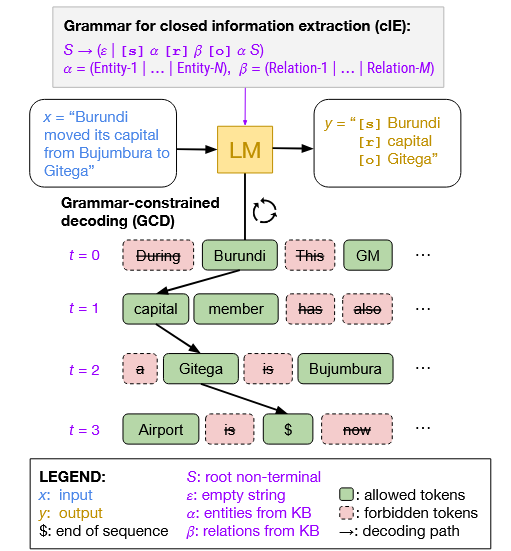
\includegraphics[width=0.45\textwidth]{Graphics/gcd.png}
\caption{Imagen extraída de \textcite{geng2023grammar}: \textit{Grammar-Constrained Decoding (GCD)} aplicado a la tarea de \textit{closed information extraction}, donde el objetivo es extraer una lista $y$ de tripletes sujeto–relación–objeto del texto de entrada $x$. Los sujetos y objetos están restringidos a ser entidades de \textit{Wikidata}, y las relaciones a ser una relación de \textit{Wikidata}. Durante la decodificación, solo se consideran continuaciones de \textit{tokens} válidas que cumplen con la gramática. Por simplicidad, se omiten los símbolos de marcador especiales \texttt{[s]}, \texttt{[r]} y \texttt{[o]} en el esquema del proceso de generación.}
\label{fig:domains}
\end{figure}

Este mecanismo es compatible con cualquier algoritmo de decodificación (como \textit{greedy decoding}, \textit{beam search}, \textit{top-$k$ sampling}, entre otros) y puede aplicarse a cualquier modelo de lenguaje autorregresivo que ofrezca acceso a su distribución de salida \textit{token} a \textit{token}. Sin embargo, es importante notar que servicios como los ofrecidos por OpenAI mediante \textit{API} no permiten acceso a dicha distribución, lo que imposibilita el uso directo de \textit{GCD} en estos contextos.

La técnica también puede combinarse eficazmente con \textit{Few-Shot Prompting}. En lugar de permitir que el modelo genere texto libre condicionado a los ejemplos del \textit{prompt}, \textit{GCD} impone una gramática que define la estructura válida de la salida esperada, restringiendo así el espacio de búsqueda y guiando al modelo hacia soluciones sintácticamente correctas. Esto permite aprovechar el conocimiento previo del modelo junto con una especificación formal del dominio de salida, lo que resulta particularmente útil en tareas estructuradas donde se requiere una alta precisión en el formato.

El enfoque de \textit{GCD} representa así una herramienta crucial para la generación segura y verificable de texto estructurado, habilitando aplicaciones en modelado de código, extracción de información, y como se explorará más adelante, en la generación de descripciones válidas en \textit{PDDL}.

\subsection{\textit{Backus-Naur Form} (\textit{BNF})}

La Notación de \textit{Backus-Naur} (\textit{Backus-Naur Form} - \textit{BNF}) surgió a finales de la década de 1950 como una herramienta formal para describir la sintaxis de lenguajes de programación. En 1959, John Backus propuso un conjunto de ``fórmulas metalingüísticas'' para definir la estructura del lenguaje \textit{ALGOL 58}, basándose en ideas de gramáticas libres de contexto \parencite{backus1959syntax}. Posteriormente, Peter Naur refinó esta notación en el informe de \textit{ALGOL 60} de 1963, denominándola ``Forma Normal de Backus'' (\textit{Backus Normal Form}) \parencite{backus1963revised}. Sin embargo, Donald Knuth sugirió renombrarla como \textit{Backus-Naur Form} para reconocer la contribución de Naur y evitar la confusión con otras formas normales existentes en teoría de lenguajes formales \parencite{knuth1964backus}.

\textit{BNF} es un metalenguaje que permite expresar gramáticas libres de contexto mediante reglas de producción. Cada regla tiene la forma:

\begin{verbatim}
<no-terminal> ::= <expresión>
\end{verbatim}

Donde \texttt{<no-terminal>} representa una categoría sintáctica y \texttt{<expresión>} define cómo se puede construir esa categoría utilizando otros símbolos terminales o no terminales. Por ejemplo, una regla podría ser:

\begin{verbatim}
<expresión> ::= <término> | <expresión> "+" <término>
\end{verbatim}

Esta notación facilita la definición precisa y estructurada de la sintaxis de lenguajes de programación, siendo fundamental en el desarrollo de compiladores y analizadores sintácticos.

\subsection{Extensión moderna: \textit{GBNF} en \texttt{llama.cpp}}

La notación \textit{Backus-Naur} (\textit{BNF}) ha sido fundamental en la definición formal de lenguajes de programación. Sin embargo, con el auge de los \textit{LLMs}, ha surgido la necesidad de formatos más expresivos y adaptados a estos nuevos contextos. En este sentido, fue introducida \textit{Georgi Gerganov's Machine Learning (GGML) Backus-Naur Form (GBNF)}, una extensión de \textit{BNF} diseñada específicamente para restringir y estructurar las salidas de los \textit{LLMs} en aplicaciones prácticas \parencite{ggml2023gbnf}.

\textit{GBNF} se implementa en el proyecto \texttt{llama.cpp}, una versión en \texttt{C++} de los modelos \textit{LLaMA} desarrollada por Gerganov. Esta notación permite definir gramáticas que los modelos deben seguir al generar texto, asegurando que las salidas cumplan con estructuras sintácticas específicas. A diferencia de \textit{BNF}, \textit{GBNF} incorpora características modernas similares a las expresiones regulares, lo que permite una mayor flexibilidad y control sobre las salidas generadas por los modelos \parencite{ggml2023gbnf}.

Aunque \textit{GBNF} no cuenta con una publicación académica formal, su documentación principal se encuentra en el repositorio oficial de \texttt{llama.cpp}, específicamente en el archivo \texttt{grammars/README.md}. Esta fuente proporciona ejemplos y directrices sobre cómo implementar y utilizar \textit{GBNF} en proyectos que requieren salidas estructuradas de modelos de lenguaje \parencite{ggml2023gbnf}.

En el contexto de esta tesis, \textit{GBNF} se utiliza como el mecanismo formal que habilita la aplicación práctica de \textit{GCD} para el modelado automático de problemas en \textit{PDDL}. Al restringir la salida de un \textit{LLM} mediante una gramática \textit{GBNF}, se garantiza que las descripciones generadas sean sintácticamente válidas conforme a la especificación del lenguaje objetivo, facilitando tanto su validación como su posterior análisis por planificadores clásicos.

\subsection{Aplicaciones Previas de \textit{GCD} en planificación automática}

\textbf{\textit{Grammar Prompting for Domain-Specific Language Generation with Large Language Models}} \parencite{wang2023grammar} propone una técnica denominada \textit{grammar prompting}, que permite a los \textit{LLMs} generar la gramática, expresada en \textit{BNF}, que seguirán sus salidas posteriores mediante \textit{GCD}. En el contexto de planificación, el modelo primero predice una gramática especializada para una tarea dada y luego genera un plan \textit{PDDL} que cumple con dicha gramática. Aunque este enfoque logra mejoras en la generación de planes sintácticamente válidos, se centra únicamente en la producción de planes, no en la generación completa de modelos de problemas de planificación.

Por otro lado, \textbf{\textit{Syntactic and Semantic Control of Large Language Models via Sequential Monte Carlo}} \parencite{loula2025syntactic} introduce un marco basado en \textit{Sequential Monte Carlo} para controlar la generación de texto por \textit{LLMs} bajo restricciones sintácticas y semánticas. Aplicado a la generación de modelos \textit{PDDL}, este enfoque utiliza una gramática \textit{STRIPS} general y se limita al dominio de \textit{Blocksworld} del \textit{benchmark Planetarium} con hasta 10 objetos, asumiendo que el estado inicial (\texttt{:init}) es proporcionado. Sus resultados experimentales brindaron indicios positivos de la utilidad de \textit{GCD} para el modelado de tareas de planificación. Sin embargo, aunque el método propuesto en el artículo permite una generación más controlada y coherente, su dependencia de información previa sobre el estado inicial restringe su capacidad para generar modelos completos a partir de descripciones en lenguaje natural. Además, no se hace una exploración a profundidad de la técnica al limitarse a un subconjunto muy reducido y solo parcialmente representativo de \textit{Planetarium}.

En contraste, esta tesis propone un enfoque que utiliza \textit{GCD} para la generación completa de modelos \textit{PDDL} (incluyendo \texttt{:init}, \texttt{:goal}, \texttt{:objects}, etc.) a partir de descripciones en lenguaje natural y del dominio \textit{PDDL} correspondiente. Más aún, se evalúa en todas las dimensiones (dominio, cantidad de objetos, nivel de abstracción, etc.) del \textit{benchmark Planetarium}. De forma adicional a la gramática general, se introducen nuevos niveles de restricción especializada que aseguran el uso exclusivo de predicados disponibles, objetos declarados y la correcta aridad y tipado de argumentos, permitiendo así una generación más precisa y aplicable a una variedad de dominios y problemas específicos.

\section{El \textit{Benchmark Planetarium}}

La evaluación moderna de modelos generados automáticamente en \textit{PDDL} requiere herramientas específicas que permitan analizar no solo la validez sintáctica del código, sino también su estructura semántica y capacidad de resolución. En esta línea, el \textit{benchmark Planetarium} \parencite{zuo2024planetarium} constituye una de las contribuciones más destacadas, al ofrecer un conjunto masivo de ejemplos texto--\textit{PDDL} junto con un protocolo de evaluación riguroso basado en estructuras de grafo intermedias. Este recurso permite evaluar la generación automática de problemas de planificación desde descripciones en lenguaje natural con criterios que trascienden la simple exactitud textual o el \textit{string matching}.

La representación central empleada por \textit{Planetarium} es el \textit{scene graph} (grafo de escena), una estructura de datos ampliamente utilizada en visión por computadora y gráficos computacionales para representar objetos, sus atributos y relaciones. Formalmente, un \textit{scene graph} es un grafo dirigido $\mathcal{G} = (\mathcal{V}, \mathcal{E})$, donde $\mathcal{V} = \mathcal{O} \cup \mathcal{P}$ incluye nodos de tipo objeto ($\mathcal{O}$) y proposición ($\mathcal{P}$), y cada arista $e \in \mathcal{E}$ tiene atributos que codifican el predicado al que pertenece, la posición del argumento en la proposición, y si la proposición corresponde al estado inicial o al estado meta. Para cada archivo de problema en \textit{PDDL}, se construyen dos grafos: uno que representa el estado inicial y otro que representa las proposiciones objetivo. Estos se combinan en un \textit{problem graph}, definido como la unión etiquetada de ambos: 

\[
\textit{ProblemGraph} = (\mathcal{O} \cup \mathcal{P}_{\textit{init}} \cup \mathcal{P}_{\textit{goal}}, \mathcal{E}_{\textit{init}} \cup \mathcal{E}_{\textit{goal}})
\]

La noción de equivalencia entre problemas se formaliza como un isomorfismo de grafos sobre los \textit{problem graphs}, es decir, una biyección entre nodos que preserve tanto la conectividad como los tipos y atributos. Esta definición permite comparar problemas generados automáticamente contra su referencia canónica sin depender del soporte textual de los archivos.

El algoritmo propuesto para verificar esta equivalencia comienza transformando cada conjunto de proposiciones en grafos de escena, completando los grafos objetivo con aristas triviales (como proposiciones que se pueden inferir verdaderas), y finalmente construyendo un \textit{problem graph} a partir de la unión. Si existe un isomorfismo entre el grafo generado y el de referencia, se considera que el problema es estructuralmente equivalente y, por tanto, correcto.

El conjunto de datos de \textit{Planetarium} incluye más de 100\,000 pares texto--\textit{PDDL}, generados proceduralmente a partir de plantillas que combinan configuraciones (subtipos de estados o subtareas específicas) de los estados iniciales y objetivos. Los dominios utilizados son \textit{Blocksworld}, \textit{Gripper} y \textit{Floor-Tile}, elegidos por su uso extensivo en la literatura y su dificultad inherente. Cada problema contiene tanto una descripción en lenguaje natural como una instancia en \textit{PDDL} construida a partir de la combinación de las plantillas predefinidas. La generación automática varía sistemáticamente la abstracción de las descripciones textuales (desde descripciones explícitas hasta resúmenes abstractos de estados) y el tamaño de los problemas medido por la cantidad total de proposiciones u objetos.

\begin{figure}[H]
\centering
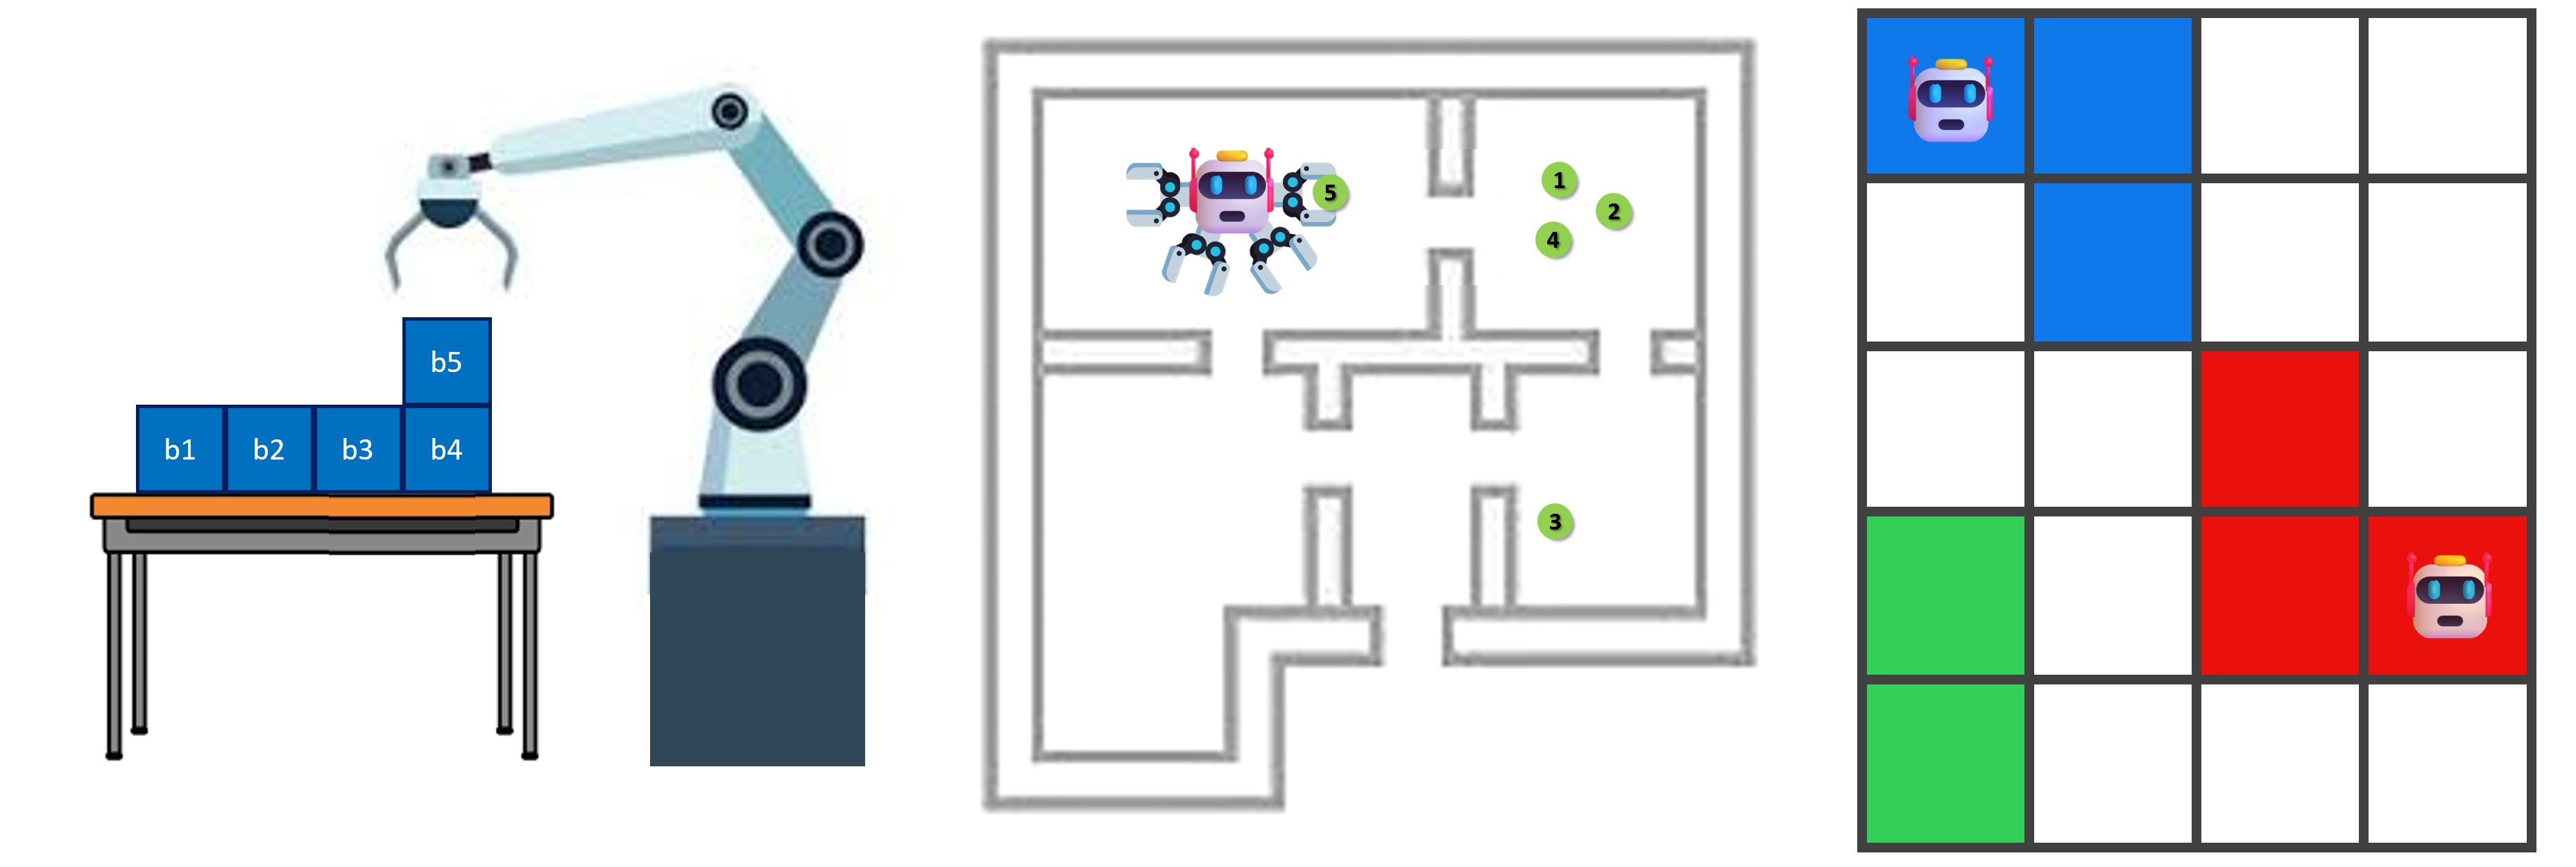
\includegraphics[width=0.8\textwidth]{Graphics/domains.png}
\caption{Dominios de problemas de planificación del \textit{benchmark Planetarium}, de izquierda a derecha: \textit{Blocksworld}, \textit{Gripper} y \textit{Floor-Tile}}
\label{fig:domains}
\end{figure}

El protocolo de evaluación del dataset considera tres métricas: el número de modelos sintácticamente válidos, el número de modelos solubles y el número de modelos correctos. Un modelo es considerado sintácticamente válido si es analizable por un \textit{parser} de \textit{PDDL}, y es posible extraer desde su salida un problema en \textit{PDDL} válido y convertirlo en un grafo estructuralmente bien formado. La solubilidad se computa determinando la existencia de un plan válido que lleva desde el estado inicial al estado objetivo, utilizando para ello planificadores específicos para los dominios \textit{Blocksworld} y \textit{Gripper}, y \textit{Fast Downward} para problemas del dominio \textit{Floor-Tile}. Finalmente, un problema se considera correcto si, siendo sintácticamente válido y soluble, es también estructuralmente equivalente al problema original según el algoritmo de isomorfismo de grafos. Para asegurar la validez de los planes generados, todos los resultados se verifican con la herramienta \textit{VAL}.

\begin{figure}[H]
\centering
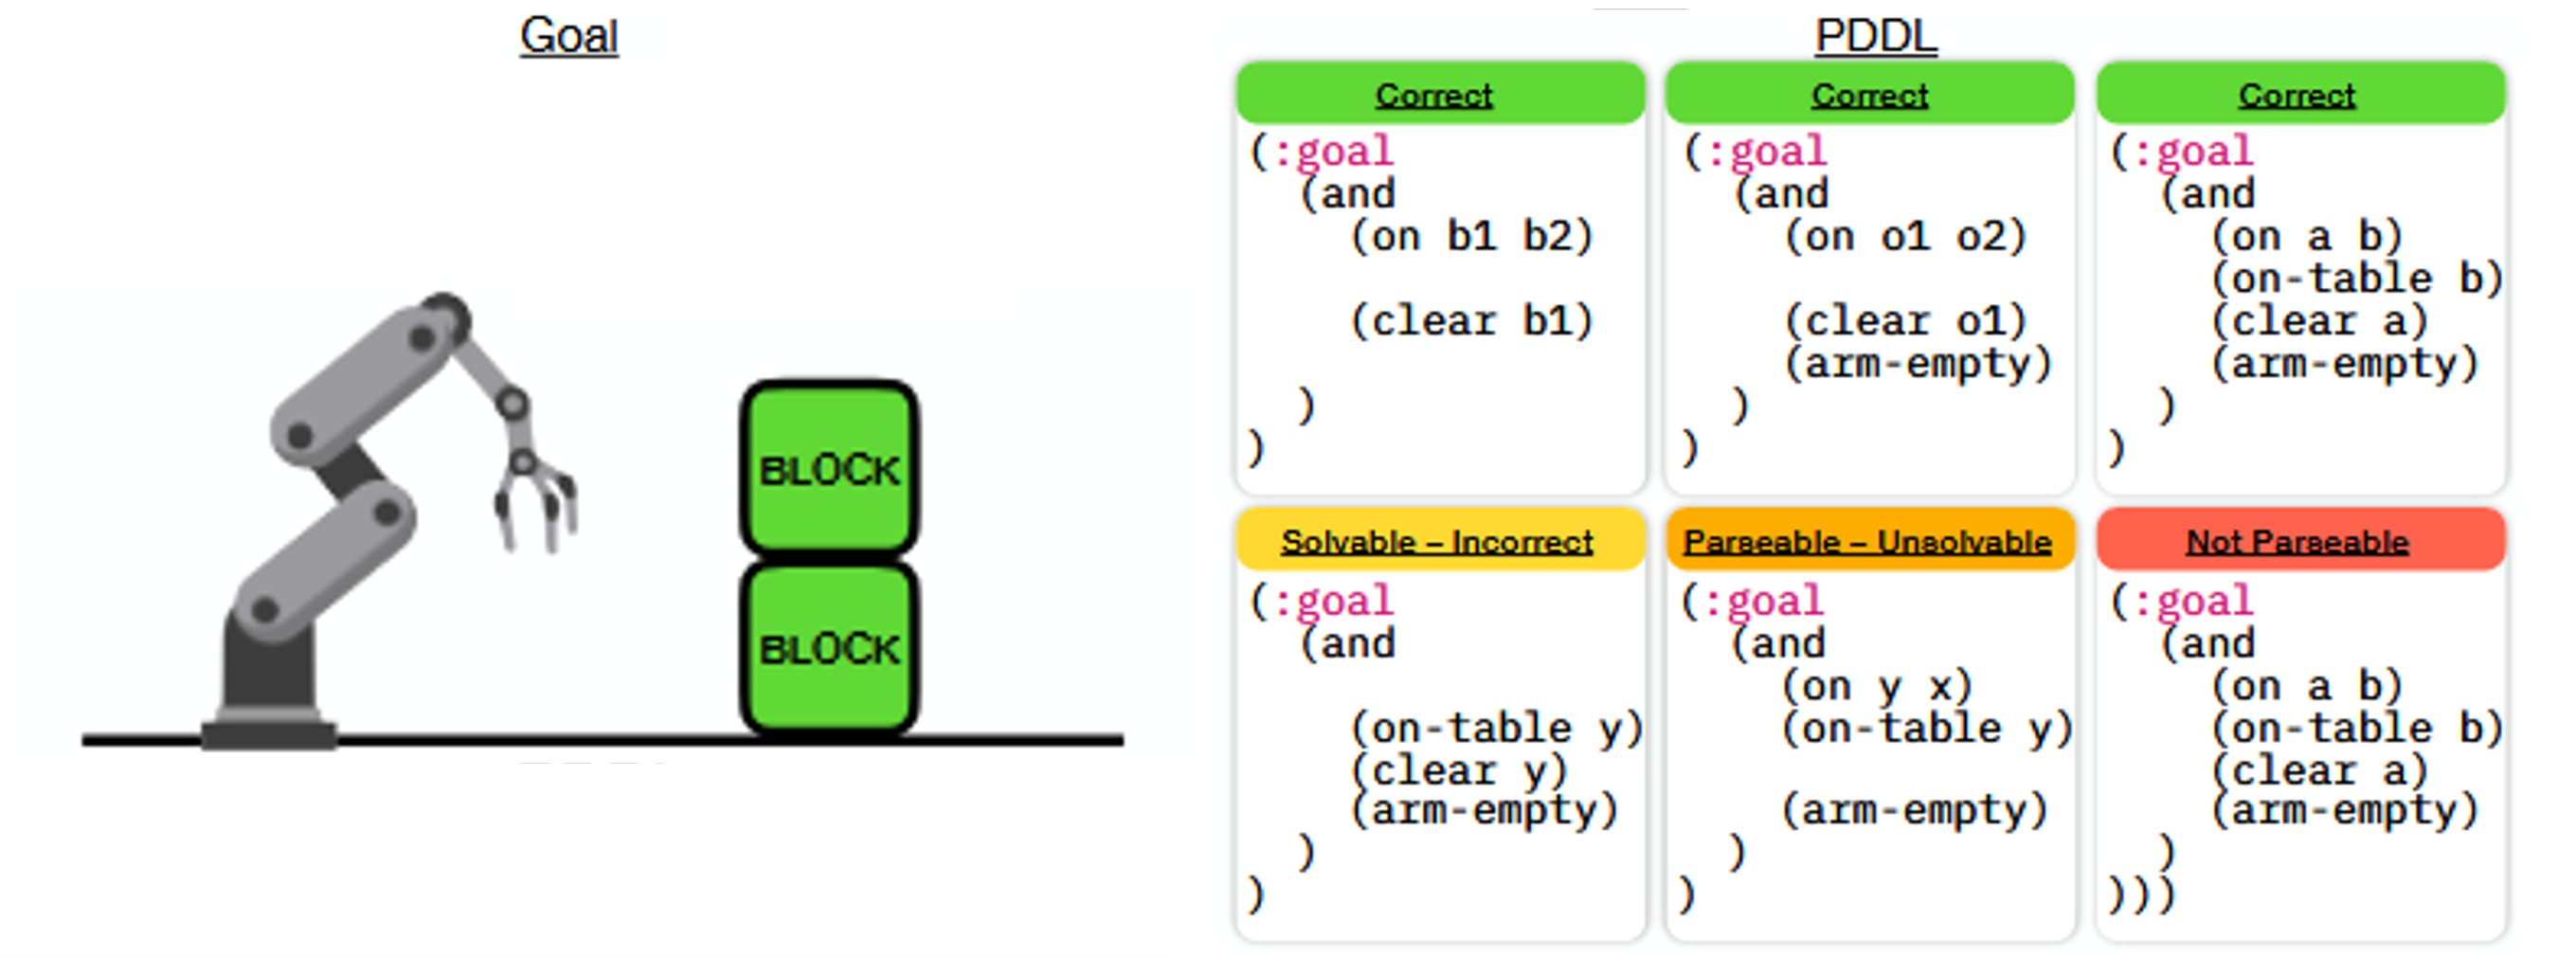
\includegraphics[width=0.9\textwidth]{Graphics/planetarium.png}
\caption{Imagen extraída del \textit{paper} de \textit{Planetarium} \parencite{zuo2024planetarium}: ejemplo de cómo un único objetivo de planificación puede corresponder a múltiples estados objetivos \textit{PDDL} correctos. Todos los objetivos \textit{PDDL} en la fila superior representan la meta mostrada correctamente. La fila inferior ilustra objetivos \textit{PDDL} con diferentes tipos de errores, mostrando instancias que son solubles (un planificador puede generar un plan, pero para un problema de planificación diferente), sintácticamente válidos (la sintaxis \textit{PDDL} es correcta pero no producirá ningún plan con un planificador) e inválidos (contiene errores de sintaxis).}
\label{fig:planetarium}
\end{figure}

Este protocolo permite una evaluación robusta de modelos basados en lenguaje natural y ofrece un \textit{baseline} reproducible para medir avances en la generación automática de modelos de planificación.

\section{Conclusiones}

Este capítulo ha presentado un recorrido exhaustivo por los fundamentos, avances y desafíos actuales en el campo de la \textit{planificación automática}, así como por las oportunidades emergentes que surgen del uso de \textit{LLMs} para la generación estructurada de modelos en \textit{PDDL}. 

En conjunto, se evidencia que, si bien los \textit{LLMs} poseen un enorme potencial para tareas de planificación estructurada, su aplicación directa a la generación de modelos \textit{PDDL} enfrenta barreras significativas de robustez y validación. Las técnicas revisadas —aprendizaje experiencial, decodificación gramatical, evaluación estructural con \textit{Planetarium}— ofrecen elementos clave para superar estas barreras. Sobre esta base se plantea en esta tesis el diseño de un agente modelador que:
\begin{itemize}
    \item Divide el proceso de modelado en fases de razonamiento estructurado, extracción de objetos y generación de \textit{PDDL};
    \item Aprende de sus errores mediante ciclos de experiencia y reflexión;
    \item Está asistido por restricciones gramaticales explícitas mediante \textit{GCD} y \textit{GBNF};
    \item Es evaluado rigurosamente con el protocolo estructural de \textit{Planetarium}.
\end{itemize}

Este enfoque integral busca cerrar la brecha entre el poder expresivo de los \textit{LLMs} y la precisión requerida por los sistemas simbólicos de planificación, contribuyendo así a un nuevo paradigma de generación automática de modelos válidos, verificables y reutilizables en el contexto de la \textit{planificación automática}.

\chapter{Propuesta de Solución}\label{chapter:proposal}

La propuesta desarrollada en esta investigación consiste, principalmente, en un sistema compuesto por múltiples agentes especializados, cuyo objetivo es la generación automática de modelos y planes \textit{PDDL} de problemas de planificación a partir de descripciones en lenguaje natural, con foco en dominios definidos en el lenguaje \textit{STRIPS} extendido con \textit{:typing}. El diseño sigue una arquitectura jerárquica y modular, basada en el uso de \textit{LLMs} para la comprensión semántica de los problemas, junto con mecanismos de entrenamiento experiencial, razonamiento estructurado, decodificación restringida por gramáticas, retroalimentación y reflexión sobre fallos. La validez de esta propuesta se evalúa de forma rigurosa sobre el \textit{benchmark Planetarium}, que proporciona un conjunto amplio de tareas con evaluación automática de validez sintáctica, solubilidad y correctitud semántica de los modelos.

Inicialmente, se definen dos conjuntos de \textbf{\textit{baselines}}: por un lado, los \textbf{\textit{agentes planificadores}}, encargados de emitir planes directamente en formato \textit{PDDL} y, por otro, los \textbf{\textit{agentes modeladores originales} del trabajo \textit{LLM+P}}, sin razonamiento explícito ni restricción gramatical, representando el paradigma más simple de modelado asistido por \textit{LLMs}. Ambos incluyen modalidad de \textit{Zero-Shot} (sin ejemplo resuelto añadido al \textit{prompt}) y \textit{One-Shot Prompting} (con un ejemplo incluido). Estos agentes son reproducidos fielmente del trabajo \textit{LLM+P}, y adaptados a su evaluación en \textit{Planetarium}.

En contraste, los \textbf{\textit{agentes modeladores propuestos}} están compuestos por múltiples submódulos especializados opcionales, que permiten descomponer y controlar la tarea de modelado. Primero, se permite ejecutar una \textbf{fase de razonamiento estructurado} para identificar los objetos relevantes, el estado inicial y objetivos del problema. Luego, se puede llevar a cabo una \textbf{fase de extracción de objetos}, en la que se listan explícitamente los objetos que formarán parte del modelo de problema. Esta descomposición semántica permite controlar la generación mediante \textit{GCD}.

La producción final del modelo \textit{PDDL} se realiza mediante \textbf{\textit{GCD}}, que garantiza la validez sintáctica del modelo generado. Como punto de partida se utiliza una gramática \textit{GBNF}, diseñada específicamente para codificar la sintaxis del subconjunto de \textit{PDDL} utilizado. Adicionalmente, se extiende este enfoque mediante la construcción dinámica de gramáticas especializadas, que se denominarán \textbf{\textit{Domain-and Problem-Specific (DAPS)}}, a partir de los objetos (tipados o no) previamente identificados, limitando la generación a predicados con aridad y argumentos válidos en el contexto del dominio y problema. Esto se consigue especializando las reglas de producción de la gramática, utilizando los objetos extraidos en la fase previa correspondiente. La técnica de \textit{GCD} se emplea tanto en la fase final de generación como durante la etapa previa de extracción de objetos, y se distinguen mecanismos diferenciados para dominios tipados y no tipados.

Un componente principal de esta propuesta es el \textbf{\textit{agente experiencial}}, con capacidad de reflexionar sobre los intentos fallidos de modelado, y realizar un entrenamiento que le permite acumular experiencias e \textit{insights}. A través de un modelo \textit{LLM} especializado en reflexión estructurada, este agente analiza tanto los errores de \textit{parsing} como las fallas semánticas que impiden la solubilidad o equivalencia del modelo con la descripción del problema, proponiendo hipótesis correctivas que se integran en las siguientes iteraciones del agente modelador. El \textit{feedback} que alimenta esta fase se construye automáticamente mediante el cálculo de las métricas concebidas en el \textit{benchmark Planetarium}, además de variantes parciales (validez o correctitud individual de \texttt{:init} y \texttt{:goal}) mediante la manipulación del modelo \textit{PDDL} generado.

La propuesta incluye además una \textbf{fase de entrenamiento} dedicada primero a la \textbf{acumulación de soluciones correctas}, y luego a la \textbf{extracción de \textit{insights}}. En esta se recopilan tanto salidas exitosas como fallidas del agente durante la resolución de múltiples tareas, generando una base de conocimientos estructurados. Los \textit{insights} abarcan buenas prácticas de planificación y conocimiento de los dominios. La extracción se realiza mediante un agente especializado basado en \textit{LLM}, al cual se le presentan conjuntos de soluciones correctas e incorrectas para su análisis. El agente modifica su base de conocimientos mediante operaciones definidas para añadir, editar y ponderar los \textit{insights} en función de su relevancia y utilidad.

Este conocimiento se incorpora al comportamiento del agente a través de técnicas de \textbf{\textit{In-Context Learning}}. Los ejemplos de soluciones correctas presentados (\textbf{\textit{Few-Shot Prompting}}) son provistos manualmente por el experto, o se seleccionan mediante mecanismos de \textbf{\textit{Retrieval-Augmented Generation (RAG)}}. En el caso de inclusión de este módulo, las descripciones de los problemas se transforman en vectores de \textit{embeddings} de lenguaje natural que permiten recuperar los ejemplos más cercanos en el espacio semántico, del \textit{pool} de experiencias acumuladas, mediante el cálculo de \textit{cosine similarity}.

Se consideran múltiples variantes del agente con diferentes combinaciones de módulos activos o inactivos (por ejemplo, con o sin \textit{GCD}, reflexión, o \textit{RAG}). La modularidad y flexibilidad de la propuesta facilita el análisis de la influencia de estos componentes en la calidad de los resultados.

En resumen, la solución propuesta no se limita a la generación directa de modelos \textit{PDDL}, sino que incorpora mecanismos robustos de restricción sintáctica, razonamiento estructurado, aprendizaje progresivo y reflexión sobre errores. Esta integración de múltiples niveles de inteligencia simbólica permite alcanzar mejoras sustanciales en la calidad de los modelos generados, acercando el uso de \textit{LLMs} en planificación a una solución confiable y escalable. A continuación, se presenta a detalle todo el diseño de la propuesta.

\begin{figure}[H]
\centering
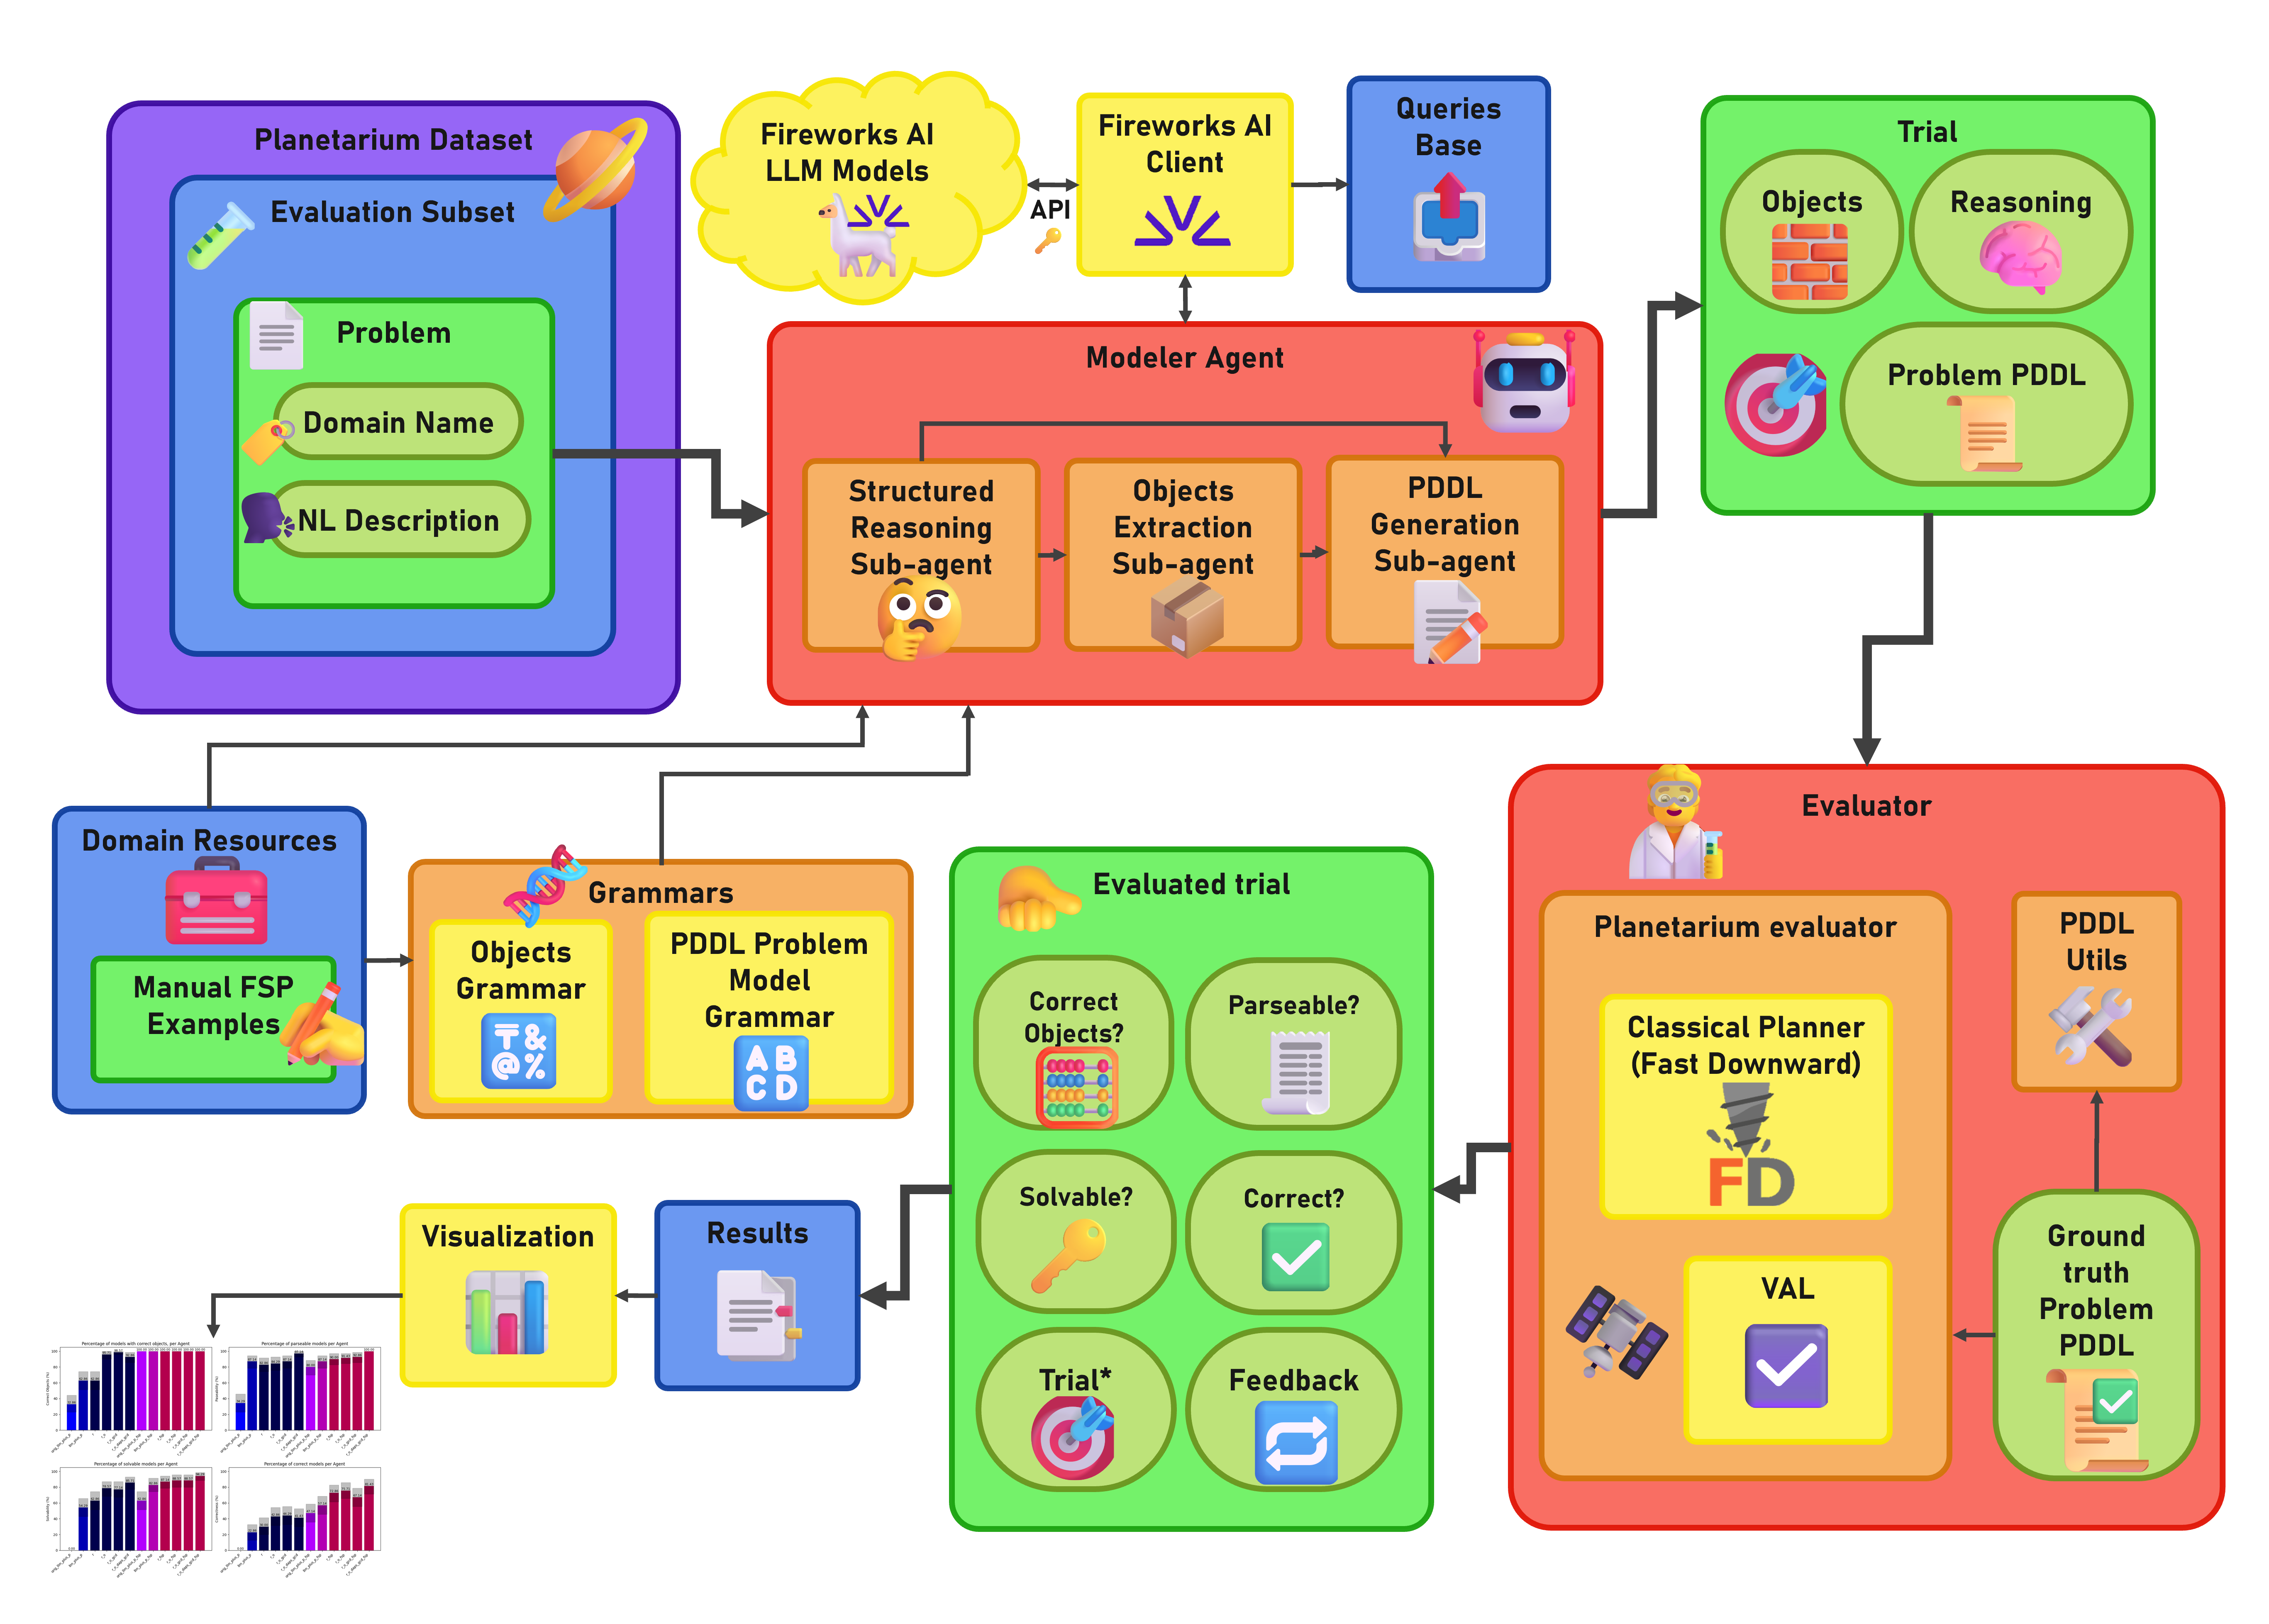
\includegraphics[width=0.9\textwidth]{Graphics/evaluation.png}
\caption{Flujo de evaluación de los agentes modeladores propuestos.}
\label{fig:objects}
\end{figure}

\section{\textit{Baselines}}

Con el fin de evaluar el impacto de los métodos propuestos para mejorar la generación de modelos \textit{PDDL}, se realiza una comparación con los agentes presentados en el trabajo \textit{LLM+P} \parencite{liu2023llm+}. Este trabajo incluye tanto un agente planificador como un agente modelador, ambos en modalidad \textit{Zero-Shot} (sin ejemplos previos), así como sus respectivas variantes \textit{One-Shot} (con un ejemplo fijo).

Se concibe una reproducción fiel de los agentes modeladores originales, realizando únicamente adaptaciones necesarias en sus \textit{prompts} para adecuarlos a los dominios del \textit{benchmark} \textit{Planetarium}. Si bien el dominio \textit{Blocksworld} coincide exactamente con el utilizado en \textit{LLM+P}, los dominios \textit{Gripper} y \textit{Floor-Tile} presentan pequeñas diferencias estructurales. Por esta razón, se adaptaron los ejemplos de \textit{FSP} manteniendo la intención de los problemas originales, pero reformulados según las variantes correspondientes de \textit{Planetarium}.

Se observó que los \textit{prompts} utilizados en el trabajo original eran considerablemente subóptimos para una evaluación automatizada en el entorno de \textit{Planetarium}, particularmente en el caso \textit{Zero-Shot}. En esta modalidad, el único contexto proporcionado al agente modelador es la descripción en lenguaje natural de las acciones disponibles. A partir de esta descripción, el agente debe inferir la totalidad de los predicados requeridos por el modelo \textit{PDDL}, incluyendo su nombre y sus argumentos. Esta condición genera una desventaja significativa, ya que la evaluación automática de \textit{Planetarium} exige que los predicados utilizados coincidan exactamente con aquellos definidos en el dominio.

En el trabajo original, este tipo de desalineaciones no representaba una limitación crítica debido a que la evaluación de los modelos \textit{PDDL} generados se realizaba manualmente. Por el contrario, en el presente trabajo se requiere una validación automática que depende estrictamente de la precisión sintáctica y semántica de los modelos generados.

En la modalidad \textit{One-Shot}, el agente recibe como entrada un ejemplo completo, pero sin la descripción explícita de todos los predicados disponibles. Aunque este enfoque ofrece al agente más información que la modalidad \textit{Zero-Shot}, todavía presenta deficiencias importantes en cobertura y comprensión semántica.

Por estas razones, se propone una reimplementación de los agentes modeladores originales, incorporando el modelo \textit{PDDL} del dominio como parte del contexto, además de una estructura de \textit{prompt} mejorada. A partir de estas versiones se pretende derivar los agentes propuestos en esta tesis, a los cuales se integran los distintos módulos de mejora.

De igual forma, los agentes planificadores son reimplementados, realizando ligeros ajustes en los \textit{prompts} con el objetivo de presentar explícitamente el formato de las acciones disponibles y adecuarlos a las particularidades de las variantes de \textit{Planetarium}.

\subsection{Agentes planificadores}

Los agentes planificadores propuestos utilizan \textit{LLMs} para resolver tareas de planificación automática. A partir de la entrada compuesta por el modelo del dominio en \textit{PDDL} y la descripción en lenguaje natural del problema, generan como salida un plan válido en el formato requerido por el validador externo \textit{VAL}, así como el conteo de \textit{tokens} consumidos durante la generación.

Basados en el enfoque propuesto en \textit{LLM+P}, se proponen dos variantes de agentes cuya única diferencia es la inclusión opcional de un ejemplo de tipo \textit{FSP} en el \textit{prompt}. Esta inclusión es modular y depende de los objetivos del experimento. Ambos agentes comparten una misma plantilla general que estructura la información presentada al modelo.

El \textit{prompt} comienza situando al modelo en el rol de un agente de planificación avanzado. Luego se introduce el dominio: su nombre, una breve descripción en lenguaje natural y el listado de acciones disponibles. Esta información proviene de una base de recursos estructurada por dominio, construida a partir de conocimiento experto. A continuación, se describe la tarea a realizar y se especifica el formato de salida esperado, también obtenido automáticamente desde la misma base.

Cuando se activa el módulo \textit{FSP}, se incorpora un ejemplo representativo del dominio, compuesto por una descripción del problema y su plan correspondiente. Este ejemplo sirve como guía contextual y es tomado directamente del conjunto de recursos por dominio.

Finalmente, se presenta el nuevo problema a resolver, tal como aparece en el \textit{dataset} de \textit{Planetarium}, y se espera que el modelo complete la sección final con el plan correspondiente.

\subsection{Agentes modeladores originales}

Los agentes modeladores originales, inspirados en la propuesta de \textit{LLM+P} \parencite{liu2023llm+}, generan como salida un archivo \textit{PDDL} que representa formalmente el problema de planificación descrito en lenguaje natural. Además, se incorpora como métrica auxiliar el número total de \textit{tokens} utilizados durante la generación, para facilitar el análisis de eficiencia.

La definición y \textit{prompt} de estos agentes varía en función de si se encuentra o no activado el módulo \textit{FSP}, que determina la presencia de ejemplos explícitos en el \textit{prompt}. Cuando dicho módulo no está activo, el modelo recibe como contexto una descripción del dominio —incluyendo sus acciones disponibles— seguida directamente por el problema en lenguaje natural a resolver. Toda esta información es obtenida desde la base de recursos por dominio, construida a partir de conocimiento experto. El modelo debe entonces generar el archivo \textit{PDDL} correspondiente, sin explicaciones intermedias.

En la modalidad con \textit{FSP}, el agente recibe primero un ejemplo completo, que incluye la descripción en lenguaje natural de un problema representativo y su respectivo archivo \textit{PDDL}. A continuación, se presenta un nuevo problema cuya descripción debe ser transformada, nuevamente, en su representación formal. Los ejemplos utilizados en esta variante fueron elaborados manualmente y adaptados desde la propuesta original de \textit{LLM+P}, ajustándolos a las especificidades de los dominios del \textit{benchmark Planetarium}.

Este diseño modular del \textit{prompt} permite estudiar el impacto de la demostración explícita de pares problema-solución sobre la calidad del modelado automático.

\section{Agentes modeladores propuestos}

La solución propuesta consiste en un agente generador de modelos \textit{PDDL}, diseñado para ser modular y extensible. A partir de una versión mejorada de los agentes modeladores originales —descritos en la sección anterior— se construye una base común utilizada tanto en los \textit{baselines} reforzados como en las variantes experimentales con módulos avanzados. Esta arquitectura permite incorporar, de manera controlada, múltiples mecanismos de mejora.

El agente base recibe como entrada el identificador numérico del problema, el dominio correspondiente y su descripción en lenguaje natural. Como salida, produce el archivo \textit{PDDL} que modela el problema y el conteo total de \textit{tokens} consumidos en la generación.

Con el objetivo de facilitar la comparación entre variantes, se adopta una estructura de \textit{prompt} estandarizada, sobre la cual se añaden condicionalmente diferentes bloques. El \textit{prompt} comienza estableciendo que el modelo actúa como un agente especializado en generación de \textit{PDDL}, y presenta al LLM el nombre y una breve descripción del dominio, junto con su definición formal en \textit{PDDL}\footnote{En el caso del dominio \textit{Floor-Tile}, con inclusión de ejemplo \textit{FSP}, se opta por omitir las acciones definidas en el \textit{PDDL} del dominio provisto, pues se observó mejor rendimiento que al agregarlos tanto en el \textit{prompt} de generación de \textit{PDDL} como en el de extracción de objetos. Esto se puede deber a que estas acciones no proveen de conocimiento relevante para esas fases, sino que representan ruido innecesario. En la fase de razonamiento, sin embargo, sí contribuye positivamente al rendimiento.}. A continuación, se enuncia la tarea: generar un modelo de problema en \textit{PDDL} que se ajuste a los requerimientos del subconjunto correspondiente, específicamente \textit{:strips} o \textit{:strips + :typing}, según la presencia o no de tipos. Estos componentes se extraen de la base de recursos de dominio instanciada por el experto.

De forma opcional, se puede incluir una indicación sobre el uso de comentarios en la sección \textit{:init} o \textit{:goal}, cuando el módulo \textit{Comments} está activado. También puede incorporarse una o más demostraciones mediante ejemplos completos (\textit{Few-Shot Prompting}, módulo \textit{FSP}), seleccionados de forma manual desde la base de recursos del dominio, o recuperados dinámicamente por un componente \textit{Retriever} en caso de la activación del módulo de \textit{RAG}.

Cada ejemplo presenta la descripción en lenguaje natural del problema, razonamientos previos y objetos relevantes si están activos los módulos \textit{Reasoning} y \textit{Objects Extraction}, respectivamente, seguidos del modelo \textit{PDDL} correspondiente.

Cuando el módulo \textit{Insights} está habilitado, el \textit{prompt} incluye un conjunto estructurado de conocimientos adquiridos previamente, organizados en tres categorías: conocimiento del mundo del dominio, y reglas o buenas prácticas de modelado de planificación, generales y específicas del dominio. Este conocimiento busca guiar al modelo, basado en experiencia acumulada.

En la parte final del \textit{prompt} se presenta el nuevo problema a resolver, expresado en lenguaje natural. Si el agente pertenece al subconjunto experiencial, y no es el primer intento sobre ese problema, se añade un bloque de reflexión que incluye la salida previa generada, el \textit{feedback} de evaluación automática, y una reflexión explícita generada por un sub-agente. Esta capacidad permite reintentos con autocrítica fundamentada, constituyendo un ciclo de mejora iterativa.

Finalmente, en presencia de los módulos de razonamiento y extracción de objetos, el \textit{prompt} puede incorporar razonamientos sobre el problema, así como la lista de objetos que deberían ser utilizados, ambos generados por sub-agentes especializados en una fase previa. Estos componentes se explican a detalle en la sección siguiente. Esta integración progresiva y jerárquica de información permite una evaluación sistemática del impacto de cada técnica sobre la calidad del modelado, respetando siempre la estructura común del \textit{prompt} para garantizar la comparabilidad entre configuraciones.

Los algoritmos de instanciación del agente modelador, su asignación de un nuevo problema a modelar, y su proceso de resolución se presentan a modo de pseudocódigos en los Anexos.

\subsection{Razonamiento}

Diversos trabajos previos han demostrado que permitir a los \textit{LLM} realizar razonamientos previos a la ejecución de una tarea puede mejorar significativamente la calidad de sus resultados. Siguiendo esta línea de investigación, se propone una fase de razonamiento, previa y separada de la generación del modelo \textit{PDDL}. Esta separación se realiza con el objetivo de modularizar el proceso, facilitar la inspección individual del razonamiento generado y permitir su reutilización en diferentes fases de modelado del problema. Además, el razonamiento explícito constituye una fuente valiosa de explicabilidad del proceso de generación automática, alineándose con principios de transparencia y trazabilidad.

El razonamiento se lleva a cabo por medio de un \textit{prompt} distinto, diseñado para inducir al \textit{LLM} a adoptar el rol de un agente especializado en análisis y razonamiento sobre la modelación de tareas de planificación. El \textit{prompt} guía de forma estructurada al modelo para razonar en tres fases bien delimitadas: \textbf{objetos}, \textbf{estado inicial} y \textbf{estado objetivo}. Estas fases reflejan directamente la estructura del modelo \textit{PDDL} de problema que se generará posteriormente, permitiendo que el razonamiento funcione como un soporte semántico directo para la construcción del modelo.

\begin{itemize}
    \item En la sección de \textbf{objetos}, se requiere enumerar de forma explícita todos los objetos mencionados o inferidos a partir de la descripción del problema. Estos objetos se corresponden con los elementos declarados en la sección \texttt{:objects} del modelo \textit{PDDL}.

    \item En la sección de \textbf{estado inicial}, el modelo debe describir detalladamente la situación inicial del problema. Se permite que el agente haga suposiciones razonables en caso de que la descripción del problema provea información ambigua o incompleta. Este contenido se traduce posteriormente en los predicados de la sección \texttt{:init}.

    \item Finalmente, en la sección de \textbf{estado objetivo}, se indica el conjunto de condiciones que deben cumplirse para considerar que el problema ha sido resuelto. Nuevamente, se induce razonamiento para completar posibles lagunas semánticas. Esta parte se traduce en la sección \texttt{:goal} del modelo \textit{PDDL}.
\end{itemize}

El \textit{prompt} utilizado establece el rol del modelo como un agente experto en razonamiento aplicado a planificación, y presenta el dominio con su descripción en lenguaje natural, su definición formal en \textit{PDDL} y una descripción textual del nuevo problema. Se solicita razonar paso a paso para resolver ambigüedades y anticipar la construcción del modelo \textit{PDDL}, mediante tres párrafos concisos con la intención anteriormente descrita. Se permite la inferencia explícita en caso de información incompleta, y se enfatiza que no debe razonarse sobre la planificación en sí, sino únicamente sobre la representación del problema. De manera análoga al \textit{prompt} principal, pueden añadirse ejemplos previos (\textit{FSP}), \textit{insights}, o reflexiones de intentos anteriores, dependiendo de los módulos activos.

\subsection{Extracción de Objetos}

Con el objetivo de anclar de forma más precisa la generación del modelo \textit{PDDL}, se propone una fase adicional de extracción estructurada de los objetos que participan en el problema de planificación. Esta fase no solo permite listar de forma clara y detallada los objetos que forman parte de los predicados en las secciones \texttt{:init} y \texttt{:goal}, sino que también facilita la construcción de una gramática más restrictiva para el \textit{GCD}. La salida del modelo en esta fase también es restringida mediante una gramática especializada. Ambas se explican a detalle en la siguiente sección.

La extracción de objetos se realiza como una etapa independiente y posterior a la fase de razonamiento (cuando esta se encuentra activa), permitiendo aprovechar directamente la información inferida en dicha fase y garantizar la consistencia entre ambos procesos. Los objetos extraídos, así como sus posibles tipos, son representados en formato \textit{JSON}, de forma estructurada y con el nivel de detalle necesario para apoyar tanto la generación posterior del \textit{PDDL} como el uso de técnicas que dependen del conocimiento explícito de la estructura del problema.

El \textit{prompt} empleado define al modelo como un agente especializado en extracción de objetos, y presenta el dominio con su descripción en lenguaje natural y su definición formal en \textit{PDDL}. Luego, se introduce el problema a resolver, y se solicita generar una lista completa de objetos relevantes en formato \textit{JSON}. Si el dominio es tipado, se indica que los objetos deben agruparse por tipo. Además, dependiendo de los módulos activos, el \textit{prompt} puede incluir ejemplos previos (\textit{FSP}), razonamiento generado previamente, o información proveniente de intentos fallidos anteriores. En particular, la reflexión sobre fallos se incluye solo si no está activa la fase de razonamiento, ya que agregar el resultado de ambas sería redundante.

\section{\textit{Grammar-Constrained Decoding (GCD)}}

Con el objetivo de asegurar la correctitud sintáctica de los modelos \textit{PDDL} generados, se propone el uso de la técnica de \textit{GCD}. Esta técnica permite imponer una gramática libre de contexto a la salida generada por un modelo de lenguaje, garantizando que la estructura del texto producido respete determinadas reglas sintácticas.

Los modelos de \textit{Fireworks AI}, utilizados en este trabajo, soportan de forma nativa la inclusión de gramáticas \textit{GBNF} a través de su \textit{API}. En el presente trabajo, la técnica de \textit{GCD} es empleada para dos propósitos fundamentales: la generación de modelos \textit{PDDL} de problema y la extracción estructurada de objetos, descrita previamente.

\subsection{\textit{GCD} para generación de modelos \textit{PDDL} de problema}

El primer paso consiste en construir una gramática general en formato \textit{GBNF} que cubra el subconjunto de \texttt{:strips + :typing} del lenguaje \textit{PDDL} para modelos de problema. Para ello, se parte de la definición original en \textit{BNF} de \textit{PDDL 3.1} \parencite{kovacs2011bnf}, la cual es filtrada y adaptada cuidadosamente para ajustarse tanto al subconjunto requerido como al formato \textit{GBNF} exigido por el sistema.

Durante este proceso se definen varios niveles de especificidad en la aplicación de la gramática:

\begin{itemize}
    \item \textbf{Base:} se define una gramática general válida para todo dominio que utilice el subconjunto \texttt{:strips + :typing}.
    \item \textbf{Restricción por dominio:} se limita el conjunto de predicados permitidos en las secciones \texttt{:init} y \texttt{:goal} a los definidos por el dominio correspondiente.
    \item \textbf{Restricción por aridad:} se asegura que la aridad de los predicados utilizados coincida exactamente con la declarada en el dominio.
    \item \textbf{Restricción por objetos:} se restringen los objetos utilizados a los declarados explícitamente en la sección \texttt{:objects} y, en dominios tipados, se verifica además que los tipos asignados a los argumentos de los predicados coincidan con los tipos de los objetos correspondientes.
\end{itemize}

El nivel de especificidad de la gramática generada depende de los módulos activos en el agente modelador. Se definen dos módulos relevantes: \textit{GCD} y \textit{DAPS} (acrónimo de \textit{Domain-and Problem-Specific}, es decir, ``específico del dominio y del problema''). Cuando el módulo \textit{GCD} está activo, la generación se realiza utilizando una gramática restringida. Si además está activo el módulo \textit{DAPS}, se incluyen las restricciones más específicas relacionadas con los predicados y/u objetos particulares del problema dado.

La estructura general de la gramática \textit{GBNF} es la siguiente:

\begin{tcolorbox}[colback=blue!5!white, colframe=blue!75!black, title=Gramática \textit{GBNF} general, fonttitle=\bfseries, breakable]
\small
\begin{verbatim}
root ::= define
define ::= "(" ws "define" ws problemDecl domainDecl requireDef 
            objectDecl init goal ")"

problemDecl ::= "(" ws "problem" ws "<Nombre del problema>" ws ")" ws
domainDecl ::= "(" ws ":domain" ws "<Nombre del dominio>" ws ")" ws
objectDecl ::= "(" ws ":objects" ws <Objetos> ws ")" ws
requireDef ::= "(" ws ":requirements" ws "<Requerimientos>" ws ")" ws
init ::= "(" ws ":init" ws initEl* ")" ws
initEl ::= literal
goal ::= "(" ws ":goal" ws preGD ")" ws

<Producción de literal>
<Producción de fórmula atómica>

preGD ::= "(and" ws GD+ ")"
<Producción de GD>

<Producciones de los objetos>
ws ::= [ \t\n]*
\end{verbatim}
\end{tcolorbox}

Los elementos entre signos \texttt{<...>} representan fragmentos variables que dependen del problema de planificación, del dominio y de los módulos activos:

\begin{itemize}
    \item \texttt{<Nombre del problema>} y \texttt{<Nombre del dominio>} se determinan a partir del problema específico que se desea modelar.
    \item \texttt{<Requerimientos>} toma el valor \texttt{:strips :typing} si el dominio está tipado, y \texttt{:strips} en caso contrario.
    \item \texttt{<Producción de literal>} y \texttt{<Producción de GD>} varían según la inclusión del módulo \textit{Comments}, que permite añadir comentarios en el modelo \textit{PDDL}. 
\end{itemize}

Si el módulo \textit{Comments} no está activo, las producciones son:

\begin{tcolorbox}[colback=blue!5!white, colframe=blue!75!black, title=Producciones sin módulo \textit{Comments}, fonttitle=\bfseries, breakable]
\small
\begin{verbatim}
literal ::= atomicFormula ws
GD ::= atomicFormula ws
\end{verbatim}
\end{tcolorbox}

En caso contrario, se añade la posibilidad de insertar comentarios al inicio de cada predicado:

\begin{tcolorbox}[colback=blue!5!white, colframe=blue!75!black, title=Producciones con módulo \textit{Comments}, fonttitle=\bfseries, breakable]
\small
\begin{verbatim}
literal ::= comment atomicFormula ws | atomicFormula ws
GD ::= comment atomicFormula ws | atomicFormula ws
comment ::= ";" [^\n]* "\n"
\end{verbatim}
\end{tcolorbox}

\subsection{Componentes específicos según inclusión del módulo \textit{DAPS}}

Los componentes variables de la gramática \textit{GBNF} ---específicamente \texttt{<Objetos>}, \texttt{<Producciones de los objetos>} y \texttt{<Producción de fórmula atómica>}--- dependen directamente de la activación o no del módulo \textit{DAPS}. A continuación se describen detalladamente ambos escenarios.

\subsubsection{Sin inclusión del módulo \textit{DAPS}}

Cuando el módulo \textit{DAPS} no está activo, la gramática permite una mayor libertad en la generación del modelo \textit{PDDL}, admitiendo cualquier nombre para objetos y tipos. Los fragmentos relevantes son los siguientes:

\begin{tcolorbox}[colback=blue!5!white, colframe=blue!75!black, title=Fragmento \texttt{<Objetos>} sin \textit{DAPS}, fonttitle=\bfseries, breakable]
\small
\begin{verbatim}
typedList
\end{verbatim}
\end{tcolorbox}

\begin{tcolorbox}[colback=blue!5!white, colframe=blue!75!black, title=Producciones de los objetos sin \textit{DAPS}, fonttitle=\bfseries, breakable]
\small
\begin{verbatim}
typedList ::= <typedList RHS>
type ::= "(either" primitiveType+ ")" | primitiveType
primitiveType ::= name | "object"

name ::= letter anyChar*
letter ::= [a-zA-Z]
anyChar ::= letter | digit | "-" | "_"

digit ::= [0-9]
\end{verbatim}
\end{tcolorbox}

El componente \texttt{<typedList RHS>} (\textit{Right-Hand Side - RHS}) depende de si el dominio es tipado:
\begin{itemize}
    \item En dominios tipados: \texttt{(name ws)+ "-" ws type ws)+}
    \item En dominios no tipados: \texttt{(name ws)*}
\end{itemize}

Finalmente, la producción de fórmulas atómicas también es completamente general:

\begin{tcolorbox}[colback=blue!5!white, colframe=blue!75!black, title=Producción de fórmula atómica sin \textit{DAPS}, fonttitle=\bfseries, breakable]
\small
\begin{verbatim}
atomicFormula ::= "(" name (ws object)* ")"
\end{verbatim}
\end{tcolorbox}

Esta formulación no impone restricciones sobre el conjunto de predicados permitidos, ni sobre su aridad o los tipos de argumentos, por lo que es más propensa a errores semánticos, aunque garantiza la sintaxis básica.

\subsubsection{Con inclusión del módulo \textit{DAPS}}

La activación del módulo \textit{DAPS} permite restringir fuertemente la generación, ajustándola al dominio y problema específicos. Para ello, se utilizan tanto los predicados definidos en el dominio, incluyendo su aridad (o tipos de argumentos en caso de dominios tipados), como los objetos obtenidos durante la fase de extracción estructurada.

\paragraph{Dominios no tipados}

En estos casos, \texttt{<Objetos>} se representa como una lista de nombres separados por espacio, entre comillas dobles. Por ejemplo, si los objetos extraídos de un problema de \textit{Blocksworld} son \texttt{[b1, b2, b3]} el fragmento queda:

\begin{tcolorbox}[colback=white, colframe=gray, title=Ejemplo de fragmento \texttt{<Objetos>} no tipado con \textit{DAPS}, fonttitle=\bfseries, breakable]
\small
\begin{verbatim}
"b1 b2 b3"
\end{verbatim}
\end{tcolorbox}

\texttt{<Producciones de los objetos>} se sustituye por: 
\begin{tcolorbox}[colback=blue!5!white, colframe=blue!75!black, title=Fragmento \texttt{<Objetos>} no tipado con \textit{DAPS}, fonttitle=\bfseries, breakable]
\small
\begin{verbatim}
object ::= "<obj1>" | "<obj2>" | ... | "<objn>"
\end{verbatim}
\end{tcolorbox}

Donde \texttt{<obj1>, <obj2>, ..., <objn>} son los nombres de los objetos determinados en la fase de extracción, cada uno entre comillas dobles y todos unidos mediante el operador de disyunción \texttt{|}. La producción correspondiente al ejemplo anterior restringe de forma explícita los objetos disponibles:

\begin{tcolorbox}[colback=white, colframe=gray, title=Ejemplo de producciones de los objetos no tipados con \textit{DAPS}, fonttitle=\bfseries, breakable]
\small
\begin{verbatim}
object ::= "b1" | "b2" | "b3"
\end{verbatim}
\end{tcolorbox}

\texttt{<Producción de fórmula atómica>} considera cada predicado posible y su aridad exacta.  En este caso empieza con el prefijo \texttt{atomicFormula ::=}, y por cada predicado proporcionado del dominio se construyen las opciones posibles de fórmulas atómicas, unidas por el operador de disyunción \texttt{|}. Cada opción es de la forma:
\begin{tcolorbox}[colback=blue!5!white, colframe=blue!75!black, title=Producción de fórmula atómica en dominios no tipados con \textit{DAPS}, fonttitle=\bfseries, breakable]
\small
\begin{verbatim}
"(<Nombre del predicado>"
 (ws object){<Aridad del predicado>} ")"
\end{verbatim}
\end{tcolorbox}

Donde \texttt{<Nombre del predicado>} y \texttt{<Aridad del predicado>} se sustituyen por sus valores correspondientes. Por ejemplo, para el predicado \texttt{(on ?x ?y)} del dominio \textit{Blocksworld}, se construye el siguiente fragmento:

\begin{tcolorbox}[colback=white, colframe=gray, title=Ejemplo de producción de fórmula atómica con \textit{DAPS} (no tipado), fonttitle=\bfseries, breakable]
\small
\begin{verbatim}
atomicFormula ::= "(on" ws (object){2} ")"
\end{verbatim}
\end{tcolorbox}


\paragraph{Dominios tipados}

En dominios que incluyen tipado, \texttt{<Objetos>} se organiza por tipo, de la forma:

\begin{tcolorbox}[colback=blue!5!white, colframe=blue!75!black, title=Objetos en dominios tipados con \textit{DAPS}, fonttitle=\bfseries, breakable]
\small
\begin{verbatim}
"<Objetos de tipo 1> <Objetos de tipo 2> ... <Objetos de tipo m>"
\end{verbatim}
\end{tcolorbox}

Donde cada fragmento \texttt{<Objetos de tipo i>} es una lista con los nombres de los objetos de dicho tipo, y terminada con el sufijo \texttt{- <Nombre del tipo>}. Por ejemplo, en  \textit{Floor-Tile}, sean los objetos extraídos:

\begin{tcolorbox}[colback=white, colframe=gray, title=Ejemplo de \texttt{<Objetos>} en dominios tipados con \textit{DAPS}, fonttitle=\bfseries, breakable]
\small
\begin{verbatim}
{
	"tile": ["tile1", "tile2", "tile3", "tile4"],
	"robot": ["robot1", "robot2"],
	"color": ["color1"]
}
\end{verbatim}
\end{tcolorbox}

El fragmento queda:

\begin{tcolorbox}[colback=white, colframe=gray, title=Fragmento \texttt{<Objetos>} en dominios tipados con \textit{DAPS}, fonttitle=\bfseries, breakable]
\small
\begin{verbatim}
"tile1 tile2 tile3 tile4 - tile robot1 robot2 - robot color1 - color"
\end{verbatim}
\end{tcolorbox}

Las producciones de objetos y de fórmulas atómicas se restringen, además, en función de los tipos esperados por los predicados.

Esto permite al modelo generar únicamente estructuras válidas desde el punto de vista sintáctico y semántico, respetando tanto los tipos como las aridades esperadas.

\texttt{<Producciones de los objetos>} es un conjunto de producciones (una por cada tipo del dominio) separadas por líneas de la forma:
\begin{tcolorbox}[colback=blue!5!white, colframe=blue!75!black, title=Producciones de los objetos por tipo (tipado con \textit{DAPS}), fonttitle=\bfseries, breakable]
\small
\begin{verbatim}
obj-<Nombre del tipo> ::= "<obj1>" | "<obj2>" | ... | "<objn>"
\end{verbatim}
\end{tcolorbox}

Donde \texttt{<obj1>, <obj2>, ..., <objn>} son los nombres de los objetos extraídos cuya clasificación corresponde a ese tipo o a alguno de sus subtipos. Siguiendo el ejemplo anterior, el fragmento resultante sería:

\begin{tcolorbox}[colback=white, colframe=gray, title=Ejemplo de producciones por tipo, fonttitle=\bfseries, breakable]
\small
\begin{verbatim}
obj-tile ::= "tile1" | "tile2" | "tile3" | "tile4"
obj-robot ::= "robot1" | "robot2"
obj-color ::= "color1"
\end{verbatim}
\end{tcolorbox}

Estas producciones asumen que cada objeto pertenece a exactamente un tipo. Asimismo, se asume una jerarquía de tipos sin multiherencia, lo cual es una simplificación válida dado que, aunque el lenguaje \textit{PDDL} permite multiherencia, la gran mayoría de dominios utilizados en \textit{benchmarks} estándar como \textit{IPC} no la emplean. Esta suposición permite construir un árbol de herencia de tipos con \texttt{object} como raíz.

Formalmente, si se tiene un conjunto de tipos \( T \) y una relación de herencia \( \prec \subseteq T \times T \), donde \( t_1 \prec t_2 \) indica que \( t_1 \) es subtipo de \( t_2 \), entonces el conjunto de objetos incluidos en la producción \texttt{obj-\textit{t}} es:

\[
\mathcal{O}_t = \{ o \in O \mid type(o) = t' \text{ y } t' \sqsubseteq t \}
\]

donde \( \sqsubseteq \) es la clausura reflexiva y transitiva de \( \prec \), y \( type(o) \) es el tipo de \( o \).

\vspace{1em}
La \texttt{<Producción de fórmula atómica>} también se adapta para aprovechar esta estructura. Se inicia con el prefijo:

\begin{tcolorbox}[colback=blue!5!white, colframe=blue!75!black, title=Estructura general de \texttt{atomicFormula}, fonttitle=\bfseries, breakable]
\small
\begin{verbatim}
atomicFormula ::= 
\end{verbatim}
\end{tcolorbox}

y por cada predicado definido en el dominio, se añade una opción con su nombre y las producciones de objetos correspondientes a los tipos de sus argumentos. Cada opción toma la forma:

\begin{tcolorbox}[colback=blue!5!white, colframe=blue!75!black, title=Plantilla por predicado (tipado), fonttitle=\bfseries, breakable]
\small
\begin{verbatim}
"(<Nombre del predicado>" ws obj-<Tipo1> ws ... ws obj-<Tipok> ws ")"
\end{verbatim}
\end{tcolorbox}

Por ejemplo, para el predicado \texttt{(robot-at ?r - robot ?x - tile)}, la producción correspondiente sería:

\begin{tcolorbox}[colback=white, colframe=gray, title=Ejemplo \texttt{atomicFormula} para predicado tipado, fonttitle=\bfseries, breakable]
\small
\begin{verbatim}
"(robot-at" ws obj-robot ws obj-tile ws ")"
\end{verbatim}
\end{tcolorbox}

Esto permite una validación estricta no solo sintáctica, sino también semántica, al restringir los objetos posibles según su tipo esperado.

\subsection{\textit{GCD} para extracción de objetos en dominios no tipados}

Para asegurar la validez sintáctica en la fase de extracción estructurada de objetos cuando el dominio no es tipado, se construye también una gramática \textit{GBNF} dedicada a esta tarea. La gramática es diseñada para aceptar exclusivamente cadenas que representaran una estructura tipo \textit{JSON} con una sola clave llamada \texttt{objects}, cuyo valor es una lista de cadenas que representaran los nombres de los objetos:

\begin{tcolorbox}[colback=blue!5!white, colframe=blue!75!black, title=Gramática para extracción de objetos (no tipado), fonttitle=\bfseries, breakable]
\small
\begin{verbatim}
root ::= "{" dq "objects" dq ": [" obj (", " obj)* "]" "}"
obj ::= dq letter anyChar* dq

letter ::= [a-zA-Z]
anyChar ::= letter | digit | "-" | "_"
digit ::= [0-9]
dq ::= "\\\""
\end{verbatim}
\end{tcolorbox}

Este esquema asegura una estructura válida en la respuesta del modelo, acorde con el formato esperado por los módulos posteriores. Por ejemplo, en un problema del dominio \textit{Blocksworld} que involucra los bloques \texttt{b1}, \texttt{b2}, \texttt{b3} y \texttt{b4}, la salida generada por el agente tiene la forma:

\begin{tcolorbox}[colback=white, colframe=gray, title=Ejemplo de salida válida (no tipado), fonttitle=\bfseries, breakable]
\small
\begin{verbatim}
{"objects": ["b1", "b2", "b3", "b4"]}
\end{verbatim}
\end{tcolorbox}

De esta manera, la aplicación de \textit{GCD} a esta fase también garantiza una representación formalmente consistente de los objetos extraídos, lo que resulta clave para los pasos posteriores en la construcción del problema en \textit{PDDL}.

\subsection{\textit{GCD} para extracción de objetos en dominios tipados}

Cuando el dominio de planificación es tipado, se utiliza una gramática específica para la fase de extracción de objetos. Esta gramática permite representar una estructura tipo \textit{JSON} en la que cada tipo del dominio se asocia con una lista de objetos del problema actual. La gramática general propuesta es la siguiente:

\begin{tcolorbox}[colback=blue!5!white, colframe=blue!75!black, title=Gramática para extracción de objetos (dominios tipados), fonttitle=\bfseries, breakable]
\small
\begin{verbatim}
root ::= <Descripción del diccionario de objetos>
obj-list ::= "[" obj (", " obj)* "]"
obj ::= dq letter anyChar* dq

letter ::= [a-zA-Z]
anyChar ::= letter | digit | "-" | "_"
digit ::= [0-9]

tab ::= "\t"
dq ::= "\\\""
el ::= "\n"
\end{verbatim}
\end{tcolorbox}

El símbolo \texttt{<Descripción del diccionario de objetos>} se define de acuerdo con los tipos presentes en el dominio específico, y representa una cadena \textit{JSON} formateada en múltiples líneas. Cada línea corresponde a una clave del diccionario (el nombre de un tipo) y su valor asociado (una lista de objetos). La construcción completa sigue el siguiente patrón:

\begin{tcolorbox}[colback=blue!5!white, colframe=blue!75!black, title=Estructura de diccionario por tipo, fonttitle=\bfseries, breakable]
\small
\begin{verbatim}
"{\n"
	tab dq "<Nombre del tipo 1>" dq ":" obj-list "," el
	...
	tab dq "<Nombre del tipo m-1>" dq ":" obj-list "," el
	tab dq "<Nombre del tipo m>" dq ":" obj-list
"\n}"
\end{verbatim}
\end{tcolorbox}

Por ejemplo, si se considera un problema del dominio \textit{Floor-Tile} con una matriz de \(2 \times 2\) (con las celdas \texttt{tile1}, \texttt{tile2}, \texttt{tile3}, \texttt{tile4}), dos robots (\texttt{robot1}, \texttt{robot2}) y un color disponible (\texttt{color1}), la salida generada por el modelo para esta fase es:
\begin{tcolorbox}[colback=white, colframe=gray, title=Ejemplo de salida de objetos extraídos (tipado), fonttitle=\bfseries, breakable]
\small
\begin{verbatim}
{
	"tile": ["tile1", "tile2", "tile3", "tile4"],
	"robot": ["robot1", "robot2"],
	"color": ["color1"]
}
\end{verbatim}
\end{tcolorbox}

Esta salida no solo facilita el uso posterior de los objetos en la generación de modelo \textit{PDDL}, sino que también posibilita la construcción de una gramática adaptada al problema específico, como se detalló en la sección anterior.

\section{Evaluación de modelos \textit{PDDL} y planes}

Una vez generado el modelo \textit{PDDL}, se procede a su evaluación mediante las métricas proporcionadas por \textit{Planetarium} y otras métricas adicionales diseñadas específicamente para este trabajo, de carácter parcial.

La función \texttt{planetarium.evaluate} para un problema recibe como parámetros el \textit{PDDL ground truth} (referencia correcta), el \textit{PDDL} a evaluar, un valor booleano que indica si se desea evaluar la \textit{solubilidad} (\texttt{solvability}), y otro booleano para el parámetro \texttt{is\_placeholder}, que define cómo se compara el problema evaluado con la referencia. Cuando \texttt{is\_placeholder} es verdadero, la función ignora la identidad específica de los objetos, permitiendo que cualquier permutación de ellos que cumpla los estados iniciales y finales sea considerada correcta. Esto es útil para problemas abstractos o donde los objetos son intercambiables, como en el caso de construir una torre de una altura específica sin importar qué bloques se utilizan. En cambio, cuando \texttt{is\_placeholder} es falso, se evalúa que los objetos individuales en los estados inicial y final del problema evaluado correspondan exactamente a los de la referencia. Este caso considera la identidad y correspondencia precisa de los objetos involucrados en el problema. La salida de esta función consta de tres valores booleanos que indican los valores de validez sintáctica, solubilidad y correctitud del \textit{PDDL}.

Recordando brevemente el funcionamiento de esta evaluación, primero se verifica que el \textit{PDDL} sea sintácticamente válido, luego que sea posible resolverlo con un planificador automático, y finalmente que el plan generado sea correcto según la referencia establecida.

Además de estas métricas estándar, se proponen otras evaluaciones parciales que permitieron un análisis más detallado del desempeño del agente modelador:

\textbf{Se evalúa que la cantidad de objetos extraídos, agrupados por tipo en el caso de dominios tipados, coincida con la referencia}. Para esta tarea se diseñó un método sencillo que permite extraer automáticamente los objetos desde la sección correspondiente de un modelo \textit{PDDL} de problema. El método consiste en localizar la sección \texttt{:objects} y recorrerla hasta el cierre (detección de un paréntesis cerrado) almacenando los objetos definidos, incluyendo sus tipos si estos se encuentran declarados (tras un guión).

\textbf{En los casos en que el modelo \textit{PDDL} resulta sintácticamente válido pero no soluble}, se analiza la posible presencia de predicados conflictivos o contradictorios en las secciones \texttt{:init} o \texttt{:goal} o en ambas. Para ello, se generan versiones del problema en las que los predicados de una de estas secciones se replican tanto en \texttt{:init} como en \texttt{:goal}, y se evalúa la solubilidad de esta instancia con predicados idénticos en ambas secciones. De esta manera, se puede determinar si las contradicciones internas en alguno de los estados inicial o objetivo provocan la insatisfacibilidad del problema. Para la evaluación se compara el \textit{PDDL} modificado consigo mismo, tomándolo como el \textit{ground truth} y la predicción simultáneamente. Cabe destacar que no todas las contradicciones se detectan debido a limitaciones impuestas por las restricciones del dominio o el funcionamiento de los planificadores automáticos, y no se profundizó en el estudio de estas causas, pues escapan del enfoque central de esta tesis. Sin embargo, esta evaluación adicional resulta útil para identificar con mayor precisión el origen del fallo, y permite construir un \textit{feedback} (retroalimentación) más específico para guiar la reflexión y el reintento de los agentes modeladores.

\textbf{Cuando el modelo \textit{PDDL} es sintácticamente válido y soluble, pero incorrecto}, se aplica un procedimiento análogo al anterior para detectar cuál o cuáles estados (\texttt{:init} y/o \texttt{:goal}) son responsables del error. Este análisis consiste en duplicar los predicados de cada estado dentro de ambos estados (inicial y objetivo) en el \textit{PDDL} generado y en el \textit{ground truth}, y luego evaluar la correctitud en base a esta modificación. La idea fundamental es que la correctitud se determina analizando el isomorfismo entre los grafos de escena generados a partir de los estados inicial y objetivo. Al replicar los predicados, se aisla el problema y se logra detectar cuando uno de los estados generados incumple independientemente la estructura o semántica esperada. No obstante, este método no es infalible, pues existen casos en los que ambos estados resultan correctos individualmente, pero su combinación genera un problema incorrecto. Este fenómeno se observó en configuraciones específicas, denominadas en \textit{Planetarium} como \texttt{strictly\_both}: \texttt{swap} e \texttt{invert} en \textit{Blocksworld}, \texttt{swap} y \texttt{juggle} en \textit{Gripper}, y en la configuración \texttt{disconnected\_rows} en \textit{Floor-Tile}. A pesar de esta limitación, la evaluación parcial adicional proporciona información valiosa para detectar fallos más precisos y construir \textit{feedback} automático detallado que facilita la mejora iterativa de los agentes.

Dependiendo de los resultados de estas evaluaciones, se genera un texto en lenguaje natural que describe la naturaleza de los errores o confirma la correctitud del \textit{PDDL} evaluado, proporcionando así un \textit{feedback} comprensible y orientado a la mejora.

\section{Agente experiencial}

En esta tesis se diseñaron estrategias inspiradas en el trabajo presentado por \textit{ExpeL} \parencite{zhao2024expel}, que propone un enfoque para el aprendizaje autónomo en agentes basados en \textit{LLMs}. En particular, \textit{ExpeL} destaca la relevancia de una fase de entrenamiento en la que el agente recopila experiencias consistentes en soluciones correctas a problemas de planificación, así como conocimientos útiles o \textit{insights} relacionados con reglas, buenas prácticas de modelación y características específicas del dominio. Además, enfatiza la importancia de que el agente pueda reflexionar sobre los errores cometidos durante intentos fallidos para corregirlos posteriormente y potenciar así la calidad de su aprendizaje.

Siguiendo esta línea, el presente trabajo adopta esta idea para diseñar un agente capaz de acumular experiencias y extraer \textit{insights} de modelación de planificación, de manera autónoma durante una fase de entrenamiento, y luego emplearlos para mejorar la toma de decisiones en tareas no vistas.

Durante la fase de entrenamiento, el agente interactúa con el entorno mediante un proceso iterativo de prueba y error, almacenando las experiencias en un \textit{pool} o repositorio de experiencias, siguiendo la noción clásica propuesta por \parencite{lin1992self}. A partir de este \textit{pool}, el agente extrae \textit{insights} de forma similar al \textit{off-policy learning} \parencite{watkins1992q}, donde es posible aprender de comportamientos pasados para mejorar la política \textit{policy} actual. Posteriormente, durante la evaluación, el agente utiliza estas experiencias e \textit{insights} para afrontar nuevas tareas, mejorando su desempeño sin requerir ajustes adicionales en el modelo.

De esta forma, la presente investigación reutiliza y adapta el marco conceptual y metodológico de \textit{ExpeL}, demostrando la viabilidad de incorporar un agente experiencial de modelación que aprende autónomamente de sus propias interacciones, y que puede transferir ese conocimiento a nuevas tareas, aportando a la mejora continua de la generación automática de modelos \textit{PDDL}.

\begin{figure}[H]
\centering
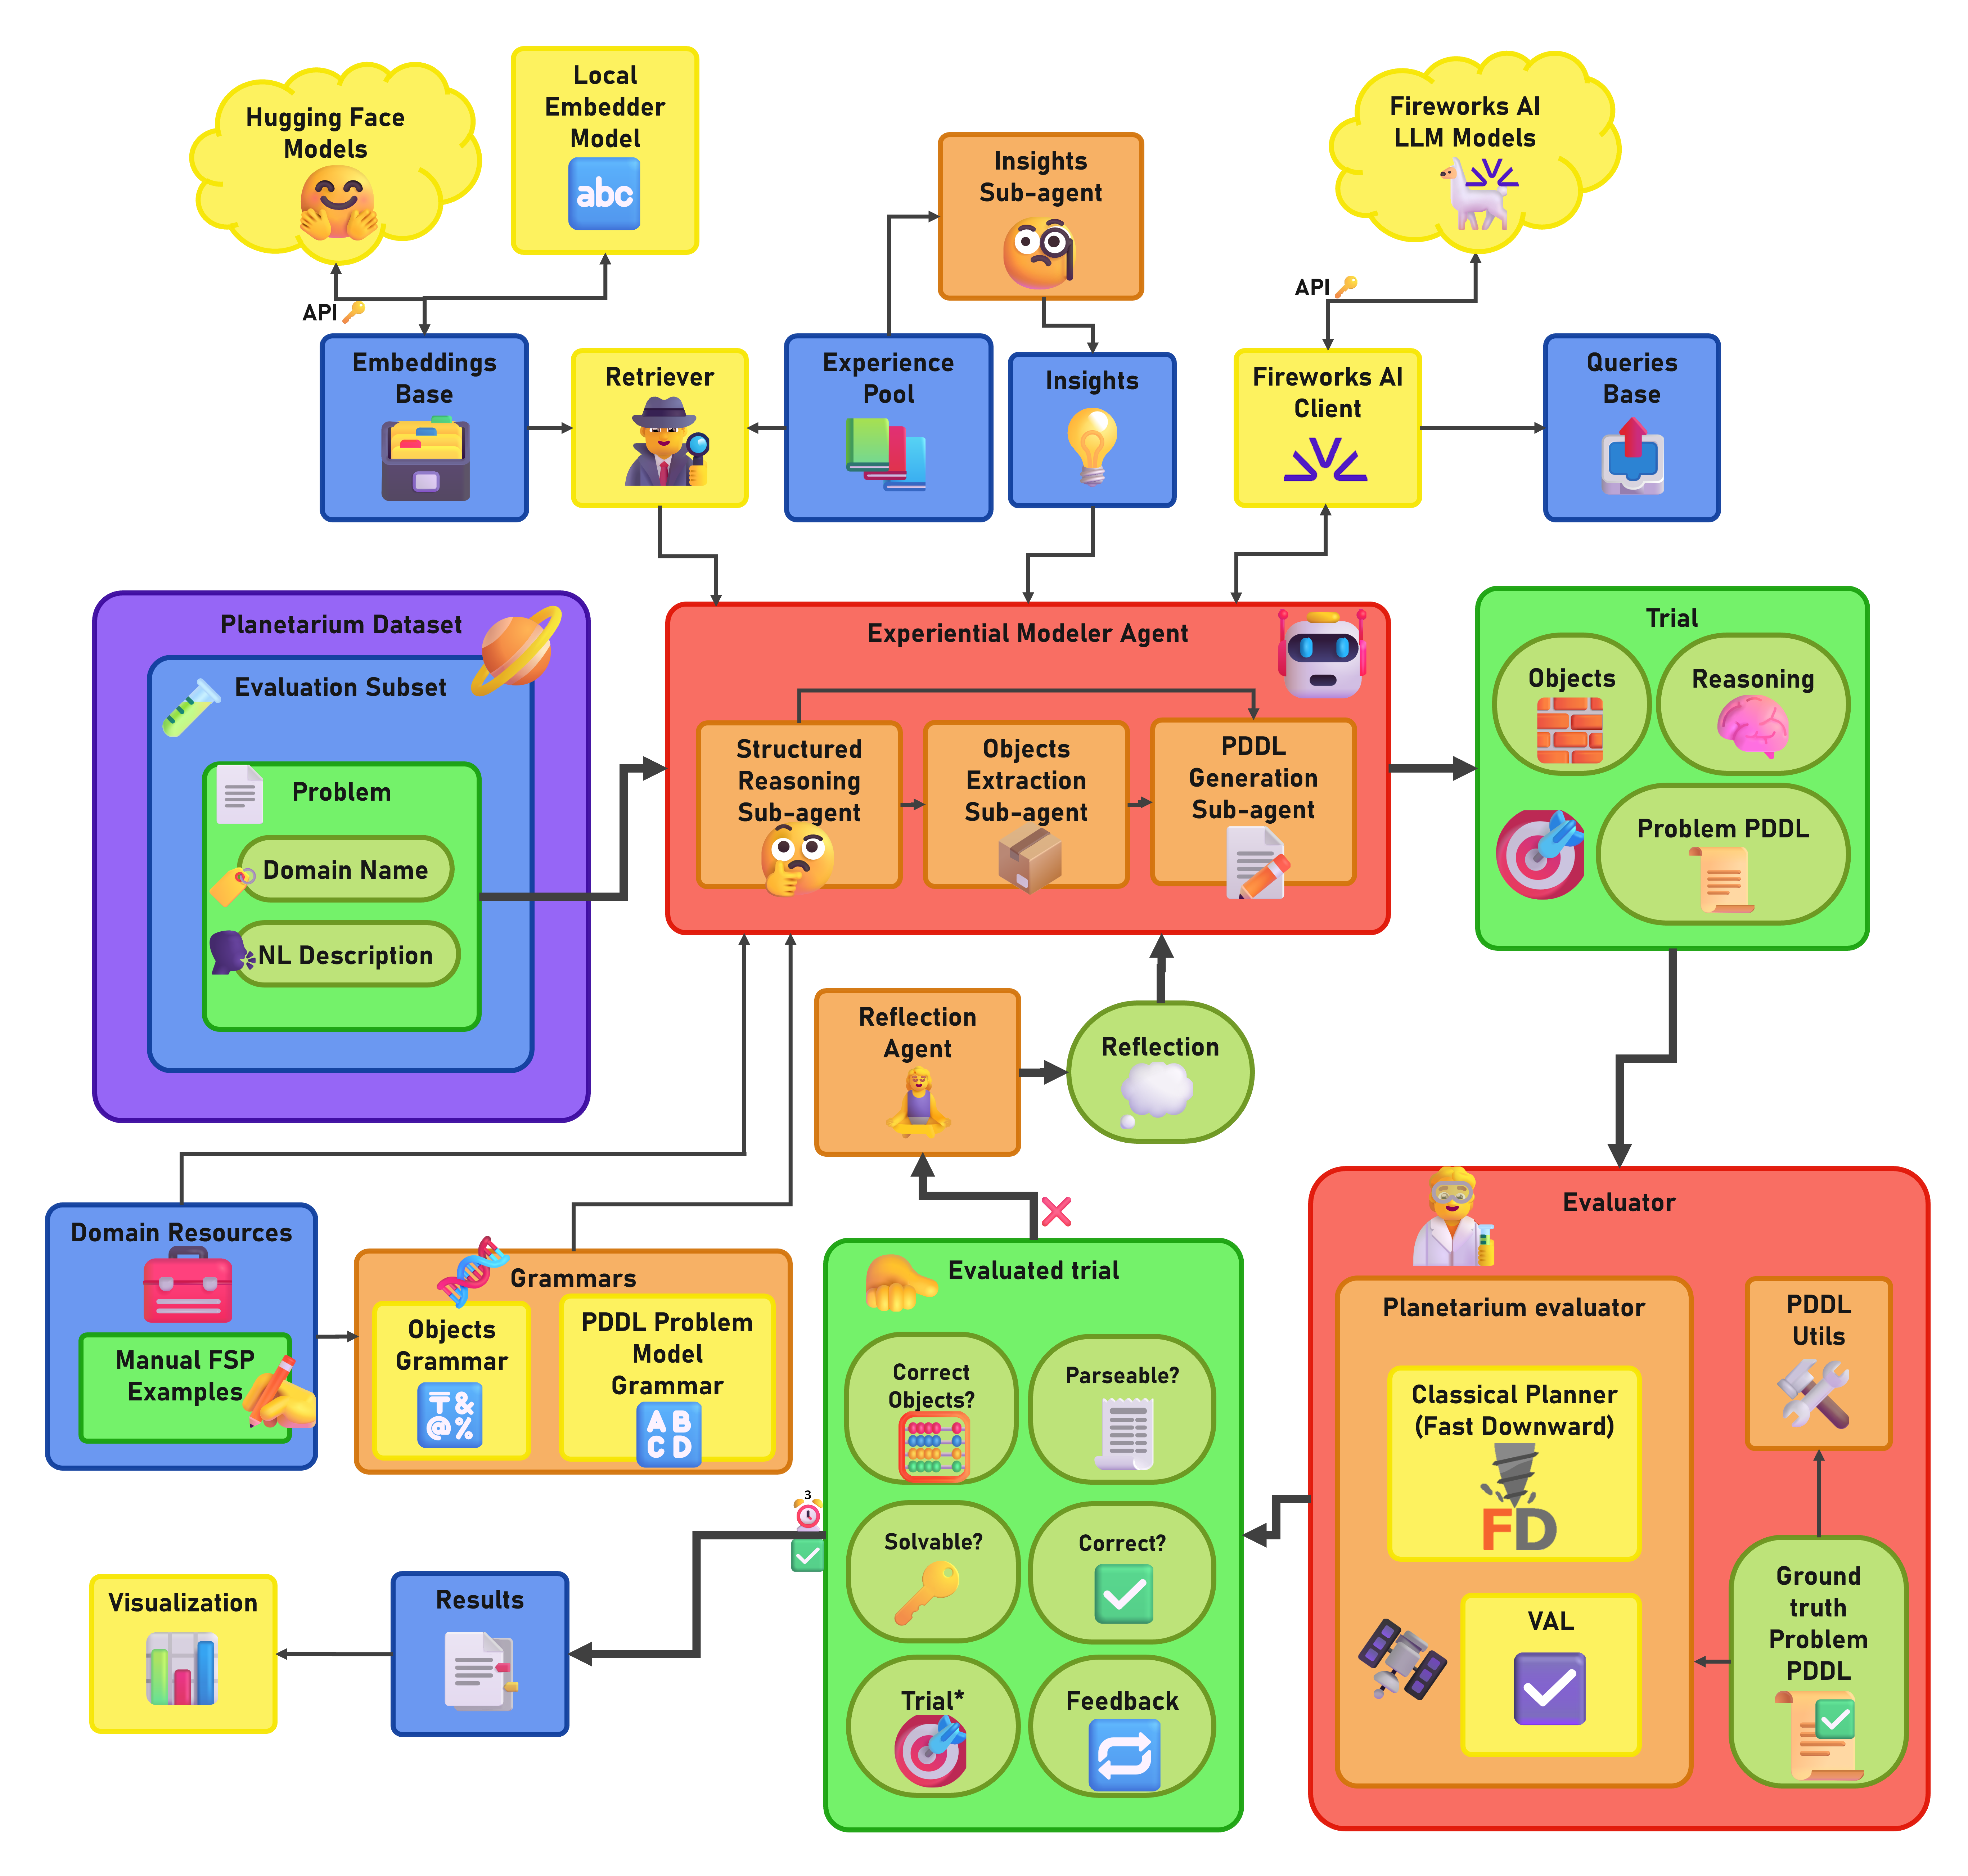
\includegraphics[width=0.9\textwidth]{Graphics/exp_evaluation.png}
\caption{Flujo de evaluación de los agentes modeladores experienciales propuestos.}
\label{fig:objects}
\end{figure}

\subsection{Reflexión}

Se propone un agente especializado en reflexionar sobre intentos fallidos de generación de modelos \textit{PDDL} de problemas de planificación. Su propósito es analizar los errores cometidos por un agente modelador al generar un modelo de problema, y proponer posibles correcciones a partir del análisis de retroalimentación proporcionado por la evaluación formal descrita en secciones anteriores.

Este agente de reflexión opera a partir de un \textit{prompt} cuidadosamente diseñado que sintetiza toda la información relevante del intento fallido, incluyendo la descripción del dominio, el modelo \textit{PDDL} del dominio, la descripción natural del problema, el razonamiento previo del agente modelador, los objetos utilizados, el modelo \textit{PDDL} generado en el intento fallido, y el \textit{feedback} obtenido tras la evaluación. Con base en esta información, el agente debe inferir la posible causa del fallo y sugerir modificaciones, de manera razonada y específica.

El \textit{prompt} instruye al modelo para que actúe como un agente experto en modelado que reflexiona sobre errores cometidos en la generación de problemas de planificación. Se le presenta un intento fallido de modelado junto con una descripción completa del contexto: dominio (nombre, explicación breve y modelo \textit{PDDL}), descripción natural del problema, razonamiento generado y objetos utilizados (si aplican), modelo generado y retroalimentación sobre el error. El agente debe considerar una jerarquía de posibles errores —errores sintácticos, problemas de solubilidad y errores semánticos— y entender que errores de menor nivel invalidan automáticamente la posibilidad de evaluar los de nivel superior (por ejemplo, un modelo con errores sintácticos no puede ser evaluado semánticamente)\footnote{Al menos bajo el alcance de esta tesis no es posible hacerlo de forma automática y determinista, pero sí sería posible que en un modelo con errores sintácticos un humano experto identifique el significado semántico subyacente y sus posibles errores.}.

El modelo debe generar un único párrafo en el que explique de forma razonada cuál pudo haber sido la causa del fallo, e indique explícitamente qué elementos deben ser corregidos: el estado inicial, el estado objetivo, o ambos. Esta reflexión se integra como una fase posterior al proceso de evaluación y puede ser utilizada por los agentes modeladores para fundamentar nuevos intentos. La capacidad de razonar sobre errores, explicarlos y proponer soluciones convierte a esta etapa en un componente crucial del ciclo iterativo de mejora basado en retroalimentación estructurada.

\section{Entrenamiento}

Con el objetivo de acumular conocimiento útil para abordar tareas futuras, se diseña un proceso de entrenamiento para el agente modelador experiencial. Este proceso consiste en dos fases bien diferenciadas: una fase de acumulación de experiencias y una fase de extracción de \textit{insights}.

La inspiración conceptual y metodológica para esta etapa proviene del trabajo presentado en \textit{ExpeL} \parencite{zhao2024expel}, el cual introdujo una estrategia sistemática de entrenamiento mediante intentos múltiples, autorreflexión y reutilización de trayectorias pasadas, tanto como ejemplos de \textit{FSP} como para la extracción de \textit{insights}.

En esta tesis se reutiliza y adapta dicho enfoque para el entrenamiento del agente modelador experiencial propuesto. Concretamente, se selecciona un subconjunto del \textit{dataset Planetarium} que tenga poca intersección con el subconjunto reservado para evaluación. Sobre este subconjunto se ejecuta un proceso iterativo, en el cual el agente intenta resolver cada una de las tareas de planificación como máximo tres veces, o hasta lograr una solución correcta.

Durante cada intento, el agente recibe como entrada la descripción natural del problema, el dominio \textit{PDDL} correspondiente, y un conjunto de ejemplos \textit{few-shot} fijos. En el primer intento, no se proporciona ninguna reflexión adicional. Sin embargo, si el intento falla, se activa el agente reflexionador descrito previamente, el cual genera una reflexión en lenguaje natural sobre las causas del fallo. Esta reflexión se incorpora al \textit{prompt} del siguiente intento, permitiendo al agente modelador considerar sus errores pasados y adaptar su estrategia en consecuencia. Este mecanismo de retroalimentación iterativa resulta clave para mejorar la tasa de éxito en intentos subsiguientes.

Todas las trayectorias generadas —ya sean fallidas o exitosas— son almacenadas en un \textit{Experience Pool} (repositorio de experiencias), que constituye una memoria a largo plazo del agente. Esta base de datos de experiencias tiene una doble función en el sistema. Por una parte, se utiliza como fuente para la recuperación de ejemplos exitosos mediante \textit{RAG} durante la fase de evaluación. Por otra, sirve como insumo para la fase de extracción de \textit{insights}, donde se analizan varias experiencias previas para identificar patrones útiles y generar recomendaciones generalizables. Esta segunda fase será detallada en la subsección siguiente.

Adicionalmente, se propone la incorporación de \textit{insights} agregados manualmente por expertos humanos, lo cual permite contrastar el conocimiento extraído automáticamente con el criterio experto, e incluso enriquecer el \textit{corpus} de recomendaciones disponibles durante la evaluación.

\begin{figure}[H]
\centering
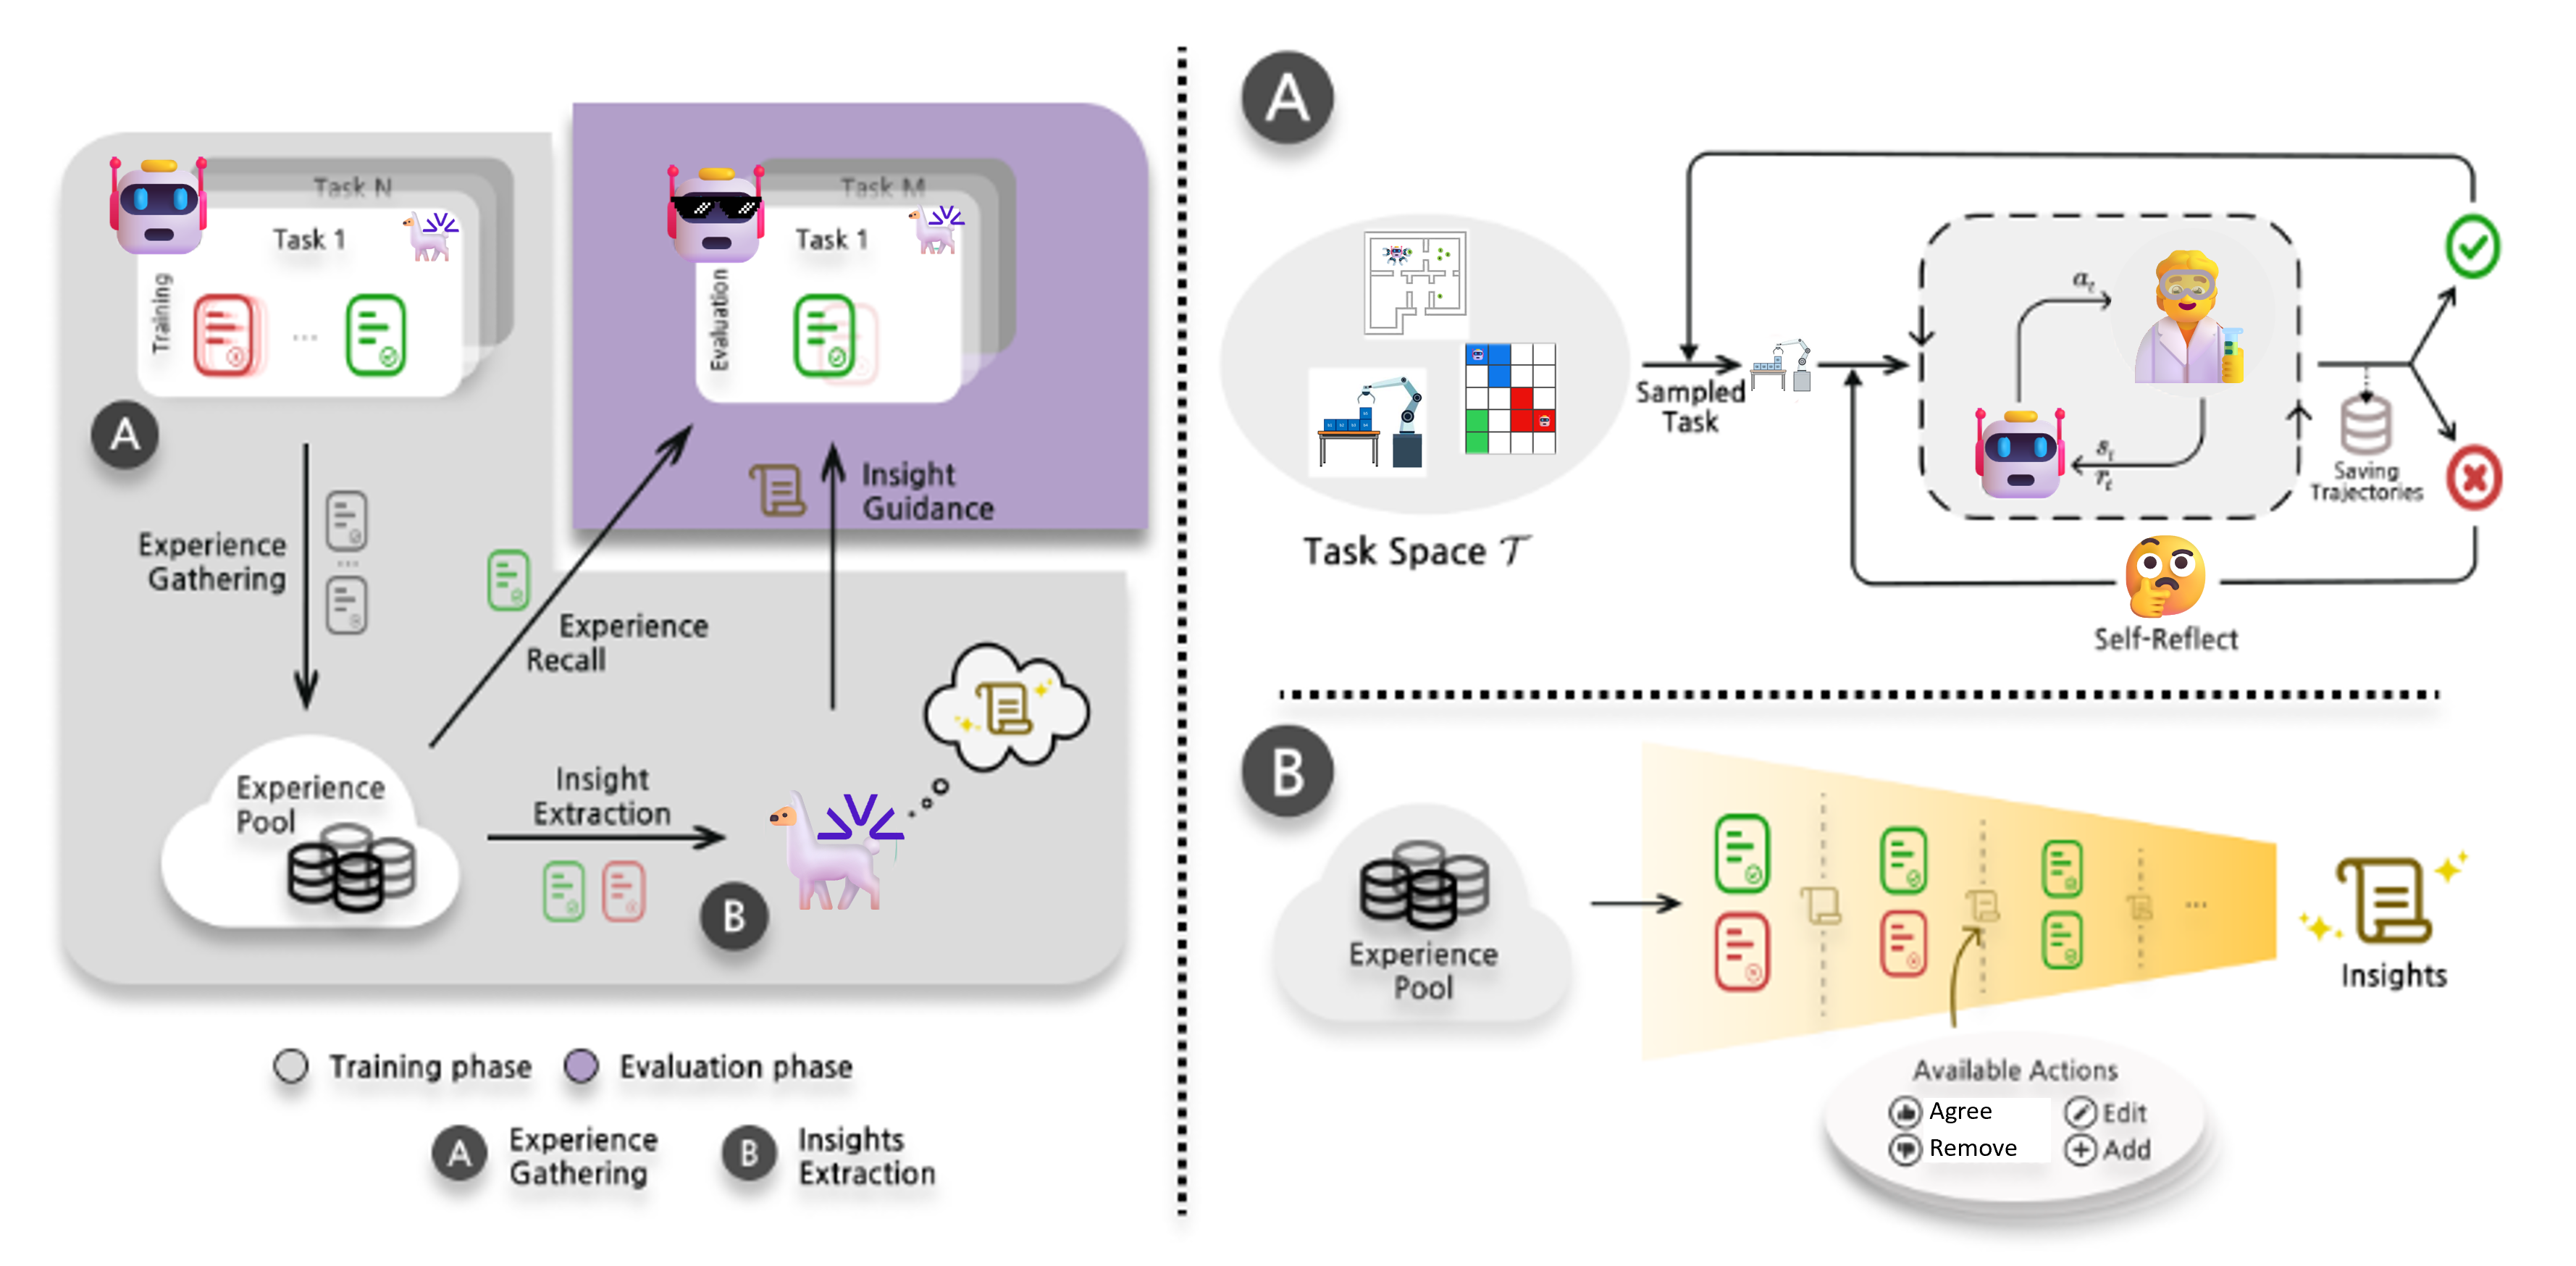
\includegraphics[width=0.9\textwidth]{Graphics/training.png}
\caption{Imagen adaptada del \textit{paper} de \textit{ExpeL} \parencite{zhao2024expel}. Izquierda: se opera en tres etapas: (1) Recolección de experiencias de éxito y fracaso en un \textit{pool}. (2) Extracción/abstracción de conocimiento entre tareas a partir de estas experiencias. (3) Aplicación de los conocimientos adquiridos y recuerdo de éxitos pasados en tareas de evaluación. Derecha: (A) Ilustra el proceso de recolección de experiencias a través del agente reflexionador, permitiendo reintentos de la tarea después de la autorreflexión sobre los fracasos. (B) Ilustra el paso de extracción de conocimiento. Cuando se le presentan pares de éxito/fracaso o una lista de $L$ éxitos, el agente modifica dinámicamente una lista existente de conocimientos $\hat{\iota}$ utilizando las operaciones \texttt{ADD}, \texttt{AGREE}, \texttt{REMOVE} y \texttt{EDIT}.}
\label{fig:training}
\end{figure}

A continuación se presenta el pseudocódigo que describe el proceso de entrenamiento:

\begin{algorithm}[H]
\caption{Entrenamiento del agente experiencial}
\label{alg:entrenamiento}
\SetKwInOut{Input}{Input}
\SetKwInOut{Output}{Output}

\Input{\\
\hspace{1em} Agente modelador \(\mathcal{A}_{\mathrm{mod}}\) \\
\hspace{1em} Conjunto de tareas de entrenamiento \(\mathcal{T}_{\mathrm{train}}\) \\
\hspace{1em} Número máximo de intentos por tarea \(Z\) \\
\hspace{1em} Indicador de continuación de entrenamiento previo: \texttt{resume} \\
\hspace{1em} Indicador de retroalimentación humana: \texttt{human\_feedback}
}
\Output{\\
\hspace{1em} Conjunto acumulado de experiencias \(B\)
}

Inicializar ruta de progreso y cargar o reiniciar estado\;
Inicializar conjunto de experiencias: \(B \leftarrow \emptyset\)\;

\eIf{\texttt{resume}}{
    Cargar índice de tarea \(i\) desde archivo de progreso\;
}{
    \(i \leftarrow 0\)\;
    Guardar progreso inicial en disco\;
}

\For{\(i = i\) \KwTo \(|\mathcal{T}_{\mathrm{train}}|-1\)}{
    \(t_i \leftarrow \mathcal{T}_{\mathrm{train}}[i]\)\;
    Inicializar reflexiones previas: \(\lambda \leftarrow \emptyset\)\;

    Llamar \(\mathcal{A}_{\mathrm{mod}}.\texttt{asignar\_tarea}(t_i)\)\;

    \For{\(z = 0\) \KwTo \(Z-1\)}{
        Resolver tarea: \(\mathcal{P}_{\pi}^{(z)} \leftarrow \mathcal{A}_{\mathrm{mod}}.\texttt{resolver}()\)\;

        Evaluar resultado: \(e_{i,z} \leftarrow \texttt{evaluar}(t_i, \mathcal{P}_{\pi}^{(z)})\)\;

        Guardar experiencia:
        \(
        B \leftarrow B \cup \texttt{store\_exp}(t_i,\ z,\ \lambda[z-1],\ \mathcal{P}_{\pi}^{(z)},\ e_{i,z})
        \)

        \eIf{\(e_{i,z}.\texttt{correct} = \texttt{True}\)}{
            \textbf{break}\;
        }{
            \eIf{\(z = Z-1\) \textbf{y} \texttt{human\_feedback}}{
                Mostrar evaluación fallida y solicitar entrada humana\;
                \(\nu_z \leftarrow \texttt{input()} \)\;
            }{
                Generar reflexión automática:
                \(
                \nu_z \leftarrow \texttt{reflect}(\mathcal{A}_{\mathrm{mod}}.P_{\mathrm{desc}},\ \mathcal{A}_{\mathrm{mod}}.D,\ \lambda,\ \mathcal{P}_{\pi}^{(z)},\ e_{i,z})
                \)
            }
            Agregar reflexión: \(\lambda \leftarrow \lambda \cup \{\nu_z\}\)\;
            Actualizar \(\mathcal{A}_{\mathrm{mod}}.\tau \leftarrow \mathcal{A}_{\mathrm{mod}}.\tau \cup (\mathcal{P}_{\pi}^{(z)},\ e_{i,z},\ \nu_z)\)\;
        }
    }
    Insertar \(B\) en base persistente\;
    Actualizar archivo de progreso con índice \(i\)\;
}
Marcar entrenamiento como completado en archivo de progreso\;

\Return \(B\)\;
\end{algorithm}

\subsection{Fase de extracción de \textit{insights}}

Una vez concluida la fase de acumulación de experiencias, se procede a una segunda fase centrada en la generación y depuración de \textit{insights}, con el propósito de sintetizar lecciones aprendidas a partir de las trayectorias recopiladas. Esta fase busca abstraer conocimientos útiles tanto específicos del dominio como generales, que puedan ser aprovechados por el agente modelador durante la evaluación para mejorar su desempeño.

En esta tesis se retoma la propuesta metodológica presentada en \textit{ExpeL} \parencite{zhao2024expel}, donde se argumenta que un agente puede analizar sus experiencias de manera sistemática para extraer conocimiento valioso. En particular, se identificaron dos mecanismos complementarios de análisis. El primero consiste en comparar una trayectoria fallida con una trayectoria exitosa sobre la misma tarea, lo cual permite identificar de forma concreta las acciones incorrectas en contraste con las correctas. El segundo mecanismo se basa en el análisis de patrones comunes entre múltiples trayectorias exitosas, provenientes de distintas tareas dentro de un mismo dominio. Esta segunda forma de análisis permite detectar buenas prácticas recurrentes, que pueden ser generalizadas como reglas efectivas de modelación.

Tomando como base dicha propuesta, se estructura la fase de extracción de \textit{insights} en dos modos operativos principales:

\begin{itemize}
  \item \textbf{Comparación entre intentos fallidos y exitosos del mismo problema.} Para cada problema del conjunto de entrenamiento resuelto con éxito, se identifican todos los intentos fallidos previos al exitoso realizados por el agente. Con estos datos se construyen pares de la forma $(\textit{incorrecto}_i, \textit{correcto})$, donde cada $\textit{incorrecto}_i$ representa una trayectoria fallida del mismo problema, y $\textit{correcto}$ corresponde a la solución exitosa. Estos pares permiten al sistema inferir causas de error específicas, reconocer desviaciones de comportamientos correctos y extraer recomendaciones de mejora concretas.
  
  \item \textbf{Comparación de múltiples soluciones correctas dentro de un mismo dominio.} Para cada dominio de planificación, se coleccionan todas las trayectorias exitosas generadas durante la fase anterior. Estas soluciones se agrupan en lotes (\textit{batches}) de tamaño configurable; en este trabajo se emplean \textit{batches} de tamaño 2. Estos lotes son utilizados para identificar patrones comunes entre problemas diferentes pero enmarcados en un mismo contexto semántico. De esta forma, se buscan regularidades y estructuras repetidas que reflejen buenas prácticas aplicables a otros problemas del dominio.
\end{itemize}

El sistema responsable de esta fase —denominado Agente de \textit{Insights}— recibe como entrada ambos conjuntos: los pares $(\textit{incorrecto}_i, \textit{correcto})$ y los \textit{batches} de trayectorias exitosas. A partir de ellos, es capaz de actualizar progresivamente su base interna de \textit{insights}, acumulando información que luego podría emplearse para guiar al agente modelador durante la evaluación.

Los \textit{insights} extraídos se clasifican en tres categorías distintas:

\begin{itemize}
  \item \textbf{Conocimiento del mundo:} Incluye información semántica específica sobre el dominio, como el significado y uso típico de predicados, restricciones físicas o abstractas implícitas, y relaciones relevantes entre objetos. Este tipo de conocimiento permite al agente comprender mejor la estructura lógica subyacente al dominio de planificación.

  \item \textbf{Reglas para la planificación en el dominio:} Contiene estrategias específicas de modelación aprendidas por observación. Por ejemplo, el uso correcto de ciertos predicados en la formulación de problemas, la inclusión necesaria de ciertos objetos o acciones, o la estructuración típica de los objetivos en ese dominio.

  \item \textbf{Reglas generales de modelación:} Se refiere a principios que resultan útiles en múltiples dominios, y que no dependen de un contexto semántico específico. Estos incluyen, por ejemplo, recomendaciones sobre la forma de declarar objetos, cómo seleccionar hechos iniciales relevantes, o patrones efectivos en la formulación de metas.
\end{itemize}

La base de \textit{insights} se inicializa vacía, y es construida de forma incremental a medida que se procesan los conjuntos de experiencias mencionados. El agente de extracción evalúa la utilidad y relevancia de cada observación, descartando aquellas poco informativas o irrelevantes, y consolidando las más consistentes o frecuentes. Esta base se diseña como un componente reutilizable, que puede enriquecer progresivamente su contenido con nuevas experiencias de entrenamiento o intervención humana experta.

Este mecanismo de análisis diferenciado de errores y éxitos, junto con la categorización estructurada del conocimiento, permite dotar al sistema de una memoria inferencial rica, orientada a facilitar la generalización y la transferencia de aprendizajes durante la fase de evaluación.

\section{Agente de \textit{Insights}}

Como se explicó en la sección anterior, los \textit{insights} representan unidades de conocimiento estructurado, útiles para la modelación de problemas de planificación automática. Cada \textit{insight}, independientemente de su tipo (conocimiento del mundo, reglas del dominio o reglas generales), se representa mediante una breve descripción textual y un valor numérico que indica su relevancia acumulada, interpretado como una medida de confianza, utilidad o frecuencia.

Con el objetivo de mantener y actualizar este conjunto de \textit{insights}, se propone un sistema especializado: el \textit{Agente de Insights}. Este agente opera sobre la base de un conjunto de acciones bien definidas que le permiten construir, refinar y filtrar progresivamente el conocimiento extraído de las experiencias almacenadas.

Este enfoque toma como referencia directa el mecanismo descrito por \textit{ExpeL} \parencite{zhao2024expel}, donde se propone iniciar con un conjunto vacío de \textit{insights}, y actualizarlo de forma iterativa a partir del análisis de pares $(\textit{fallo}, \textit{éxito})$ o listas de trayectorias exitosas, previamente recolectadas en la fase de acumulación de experiencias. En cada iteración, el modelo de lenguaje recibe alguno de estos conjuntos como contexto, y debe decidir qué operaciones aplicar sobre los \textit{insights} actuales.

Las operaciones permitidas por el agente son las siguientes:

\begin{itemize}
  \item \textbf{ADD} (agregar): introduce un nuevo \textit{insight} que no esté representado aún en la base. Este nuevo \textit{insight} es añadido con el texto sugerido por el agente, y un valor inicial de relevancia igual a 2. Esta operación permite extender el conocimiento acumulado.

  \item \textbf{EDIT} (editar): modifica el contenido textual de un \textit{insight} ya existente, con el objetivo de mejorar su claridad, generalidad o aplicabilidad. Esta operación también incrementa su valor numérico en 1, como señal de reafirmación de su utilidad tras la edición.

  \item \textbf{AGREE} (confirmar): reafirma la validez de un \textit{insight} existente, confirmando que sigue siendo relevante para los ejemplos analizados. Esta operación incrementa su valor numérico en 1.

  \item \textbf{REMOVE} (eliminar o devaluar): indica desacuerdo con un \textit{insight} actual, por considerarlo erróneo, irrelevante, redundante, demasiado específico, o \textit{superseded} (superado por otro más general o actualizado). Esta operación disminuye su valor numérico. Para controlar la sobreacumulación de \textit{insights}, se define un umbral $M$ (establecido en 10). Si el número de \textit{insights} de un tipo dado es mayor o igual a $M$, esta operación disminuye el valor numérico del \textit{insight} seleccionado en 3 unidades; en caso contrario, la disminución es de 1. Si el valor resultante no es positivo, el \textit{insight} es eliminado de la base.
\end{itemize}

Esta política de actualización se diseña para ser robusta frente a sesgos o errores puntuales en las trayectorias, permitiendo reforzar progresivamente aquellos \textit{insights} que son validados de forma reiterada en contextos distintos, y depurar los que no resultan útiles o se contradicen con ejemplos posteriores. Este diseño también considera que incluso trayectorias exitosas pueden ser subóptimas, y por tanto sus recomendaciones deben ser sometidas a verificación iterativa.

Además, para mantener la estabilidad y eficiencia del sistema, se establece un número máximo de operaciones por tipo de \textit{insight} durante cada sesión de procesamiento. En este trabajo, se fija un límite de 4 operaciones por tipo, lo cual obliga al agente a priorizar sus modificaciones más relevantes en cada interacción.

Mediante este mecanismo, se pretende que el \textit{Agente de Insights} construya de manera incremental una base de conocimientos estructurados y validados, capaz de asistir al agente modelador durante la etapa de evaluación, tanto en la selección de hechos iniciales como en la formulación de objetivos o en la verificación de consistencia semántica.

Para permitir que el agente opere sobre conjuntos complejos y estructurados de conocimiento, se concibe un \textit{prompt} parametrizable y flexible que guía el comportamiento del modelo de lenguaje durante la fase de generación o depuración de \textit{insights}. Este \textit{prompt} adopta una estructura instruccional clara, definiendo el contexto del dominio, las reglas operacionales, las limitaciones por tipo de \textit{insight}, y la información sobre los intentos previos que deben ser tenidos en cuenta.

Al igual que en agentes anteriores, algunos componentes del prompt son completados dinámicamente en función del dominio en cuestión, del estado actual de la base de \textit{insights} y de las experiencias a analizar. El nombre del dominio, su descripción breve en lenguaje natural y su correspondiente modelo en \textit{PDDL} se extraen directamente de la base de datos del dominio, y constituyen el contexto sobre el que se espera que el agente razone. Junto a ello, se incluye el conjunto actual de \textit{insights} organizados en las tres categorías establecidas (conocimiento del mundo, reglas específicas del dominio y reglas generales), presentados de forma numerada para su referencia.

El \textit{prompt} también informa al agente sobre el límite máximo de operaciones por tipo de \textit{insight}, y define de forma explícita los elementos que debe considerar al tomar decisiones, como reflexiones, retroalimentaciones de evaluación, o trayectorias exitosas y/o fallidas previas. Según el procedimiento que haya generado ese conjunto de entrada, se incorpora también una descripción del modo de extracción, y si se detecta una cantidad excesiva de \textit{insights} de cierto tipo (es decir, si se ha superado un umbral establecido), se añade una instrucción adicional que obliga al agente a priorizar operaciones de depuración o eliminación, en lugar de seguir incrementando la base de conocimiento.

Este \textit{prompt} es utilizado durante la fase de construcción del conocimiento derivado, permitiendo al agente analizar críticamente los datos acumulados y refinar su base de \textit{insights} de manera progresiva, controlada y fundamentada.

\subsubsection{Comparación de un par de intentos de un mismo problema, uno fallido y uno exitoso}

Uno de los mecanismos de extracción de \textit{insights} es la comparación directa entre un intento fallido y uno exitoso sobre el mismo problema. Este enfoque permite al agente identificar cambios clave que condujeron a una solución correcta, extrayendo lecciones reutilizables que pueden informar futuros intentos. Esta estrategia se inspira directamente en el enfoque de \textit{ExpeL}, donde se formaliza la reflexión comparativa como una técnica eficaz para detectar errores frecuentes, sistematizar buenas prácticas y fortalecer el desempeño del agente a lo largo del tiempo.

En este modo de operación, el \textit{prompt} proporcionado al agente incluye información detallada sobre ambos intentos. Para definir el contexto, se especifica que se trata de dos intentos —uno exitoso y otro fallido— de una misma tarea de planificación, en los cuales el agente modelador recibió siempre la misma descripción del dominio, el archivo \textit{PDDL} del dominio, y una descripción en lenguaje natural del problema. Esta información contextual se incluye con una redacción explícita que enmarca la tarea de contraste.

Luego, se le indica al modelo que debe enfocar su análisis en patrones, errores recurrentes o lecciones que puedan deducirse al comparar ambos intentos. El bloque posterior incluye una representación completa del intento fallido —con razonamiento y objetos seleccionados (si aplican), el modelo \textit{PDDL} generado y la retroalimentación obtenida— así como la reflexión generada tras la evaluación si esta se encuentra disponible. A continuación, se presenta también el intento exitoso con su salida generada, lo que permite una visión paralela de las decisiones tomadas antes y después de corregir los errores. Esta estructura está pensada para proporcionar un marco claro al agente, en el que puede detectar, comparar y abstraer conocimiento útil a partir de los contrastes observados.

\subsubsection{Comparación de varias soluciones correctas de distintos problemas del mismo dominio}

Además del anterior, se incorpora un modo de extracción que opera sobre múltiples intentos exitosos correspondientes a distintos problemas del mismo dominio. Este enfoque busca generalizar buenas prácticas a partir de trayectorias que han demostrado ser válidas, capturando regularidades que puedan aplicarse a nuevas instancias similares. De nuevo, este procedimiento sigue las recomendaciones de \textit{ExpeL}, donde se argumenta que las soluciones correctas también son fuentes valiosas de conocimiento estructurado.

En este caso, el \textit{prompt} indica explícitamente que todas las entradas corresponden a intentos exitosos en un mismo dominio, manteniendo el contexto —la descripción del dominio y su modelo en \textit{PDDL}— solo variando la formulación del problema en lenguaje natural, para cada tarea analizada. Esta información se incorpora consecutivamente, y prepara al agente para analizar los datos bajo un criterio común.

El conjunto de datos presentado al agente incluye varios intentos exitosos, cada uno estructurado de forma consistente, con información sobre el problema, el razonamiento realizado y los objetos determinados (si aplican), y el modelo generado. Una instrucción dada orienta al modelo a identificar patrones o lecciones presentes en estas soluciones válidas, permitiéndole extraer \textit{insights} que refuercen estrategias útiles y recurrentes dentro del mismo dominio de planificación.

\section{RAG}

Durante la fase de acumulación de experiencias, se generan múltiples soluciones correctas de modelación de problemas de planificación. Estas soluciones exitosas se estiman útiles como ejemplos de \textit{FSP} para resolver nuevos problemas, mediante \textit{RAG}.

Cuando se presenta una nueva tarea a resolver, y se requieren $k$ ejemplos de \textit{FSP}, el sistema selecciona las $k$ soluciones almacenadas en el \textit{Experience Pool} cuya descripción en lenguaje natural sea más similar a la del nuevo problema. Esta similitud se determina mediante el cálculo de \textit{embeddings} de lenguaje natural de las descripciones de los problemas, y el uso de la medida de \textit{cosine similarity} (similitud del coseno) para obtener las más cercanas.

En el capítulo de Implementación se analiza a detalle el proceso que se lleva a cabo.
\chapter{Implementación de la propuesta}\label{chapter:implementation}

\section{Estructura del proyecto}

El sistema propuesto fue implementado en \textbf{Python 3.12}, haciendo uso extensivo de bibliotecas modernas para procesamiento de lenguaje natural, planificación automática y manejo de datos. La arquitectura del código siguió un diseño modular y extensible, con componentes claramente separados por responsabilidad: agentes modeladores y planificadores, interacción con \textit{LLMs}, evaluación de modelos, entrenamiento experiencial, y recuperación semántica con \textit{RAG}. Cada módulo contó con su propia estructura de datos y utilidades específicas, lo que facilita tanto la reproducibilidad como la incorporación de mejoras o nuevas estrategias de modelado. 

Se integraron herramientas como \texttt{sentence-transformers} para \textit{embeddings} de lenguaje natural, \texttt{Fast Downward} para planificación clásica, y \texttt{VAL} para validación de planes. Las consultas a modelos de lenguaje se gestionaron mediante la \textit{API} de \textit{Fireworks AI}, y se realizó un seguimiento detallado del consumo de \textit{tokens} para evaluar la eficiencia del sistema. La base de datos del \textit{benchmark Planetarium} se almacenó en formato \textit{SQLite}, permitiendo un acceso eficiente y estructurado. 

El conjunto del sistema puede ejecutarse desde un único punto de entrada (\texttt{main.py}), facilitando la ejecución de experimentos completos de principio a fin. La estructura del proyecto implementado se presenta en el Anexo correspondiente. A continuación se describen a detalle algunos de los componentes relevantes implementados.

\section{Recursos de dominio}

Para cada uno de los dominios considerados en este trabajo, se construyó un conjunto de recursos que permitió automatizar y estandarizar los procesos de razonamiento, extracción y generación. Estos recursos fueron esenciales tanto para la etapa de entrenamiento y ajuste de los agentes modeladores, como para su evaluación. Los elementos incluidos en esta base de recursos fueron:

\begin{itemize}
    \item Un problema de ejemplo del dominio, utilizado para \textit{FSP}. Este consiste en:
    \begin{itemize}
        \item Una descripción en lenguaje natural del problema (\texttt{fsp\_ex\_nl.txt}).
        \item Un razonamiento estructurado sobre la modelación del problema (objetos, estado inicial, estado objetivo) (\texttt{fsp\_ex\_reasoning.txt}).
        \item El conjunto estructurado de objetos relevantes extraídos del problema, tipados si el dominio lo requiere (\texttt{fsp\_ex\_objects.json}).
        \item El modelo \textit{PDDL} del problema (\texttt{fsp\_ex\_pddl.pddl}).
        \item Un plan que resuelve el problema, en formato \textit{PDDL plan}, una secuencia de acciones concretas del dominio (\texttt{fsp\_ex\_plan.pddl}).
    \end{itemize}
    \item Una descripción corta del dominio en lenguaje natural (\texttt{domain\_description.txt}).
    \item Una descripción en lenguaje natural de las acciones disponibles en el dominio, incluyendo su nombre, parámetros, precondiciones y efectos (\texttt{actions\_description.txt}).
    \item La descripción de la sintaxis esperada de la salida del planificador, es decir, el formato del plan esperado (\texttt{planner\_output\_syntax.txt}).
    \item El modelo \textit{PDDL} del dominio completo (\texttt{domain.pddl}).
    \item La lista de predicados definidos en el dominio, junto con su aridad. En el caso de dominios tipados, también se indicaron los tipos de cada uno de los argumentos.
    \item La jerarquía de tipos del dominio, en caso de que este cuente con tipado.
\end{itemize}

Para facilitar el acceso y reutilización de esta información en diferentes componentes del sistema, se implementaron métodos utilitarios simples en \textit{Python} que permitieron importar y consultar dinámicamente estos recursos a partir del nombre del dominio. Esto permitió no solo una mayor modularidad en el diseño del agente modelador, sino también una integración directa con los módulos de razonamiento, extracción y validación semántica.

\section{Modelos de Lenguaje}

Todos los agentes modeladores desarrollados en este trabajo utilizan \textit{LLMs} a través de la interfaz de programación de aplicaciones (\textit{API}) provista por la plataforma \textit{Fireworks AI}. Esta plataforma permite acceder de manera flexible y configurable a modelos de última generación, incluyendo diversas funcionalidades clave que se detallan a continuación:

\begin{itemize}
    \item \textbf{Selección de modelos:} La \textit{API} ofrece acceso a distintos modelos del estado del arte. Para este trabajo se utilizó el modelo \textbf{Llama 4 Maverick Instruct (Basic)} \parencite{fireworks2025llama4maverick}. Esta decisión se debe a la buena relación entre su alta capacidad y su costo relativamente bajo en comparación con otras alternativas de similar potencia.
    
    \item \textbf{Construcción del \textit{prompt}:} Se emplea el esquema de diálogo estructurado típico en los \textit{LLMs} modernos, donde se definen dos roles: \textit{system} y \textit{user}. El \textit{system prompt} se utiliza para establecer el comportamiento general del modelo, mientras que el \textit{user prompt} contiene la tarea específica a ejecutar. Esta separación permitió modularidad y claridad en las interacciones, facilitando la adaptación del agente a diferentes subtareas de modelado. En el Anexo, sin embargo, se presentan los \textit{prompts} sin separación de roles para facilitar la lectura.

    \item \textbf{Parámetro de temperatura:} La temperatura es un parámetro que controla la aleatoriedad de la salida del modelo. Valores cercanos a 0 hacen que el modelo tienda a elegir las salidas más probables (mayor determinismo), mientras que valores mayores introducen más variabilidad y creatividad. En todos los experimentos de este trabajo se fijó la temperatura en 0, con el objetivo de aumentar la garantía de resultados deterministas y reproducibles\footnote{Aunque en teoría \emph{temperatura} $= 0$ corresponde a una decodificación puramente \emph{greedy} (seleccionando siempre el \emph{token} de mayor probabilidad), en la práctica los modelos de \emph{LLM} utilizados vía \emph{APIs} (como \emph{Fireworks AI}) pueden seguir produciendo salidas distintas en ejecuciones repetidas. Esto se debe a varios factores: (1) cálculos de punto flotante en \emph{hardware} paralelo (\emph{GPUs}) no asociativos, cuyos errores de redondeo pueden alterar la elección del \emph{token} más probable; (2) arquitecturas de mezcla de expertos (\emph{Mixture of Experts} - \emph{MoE}), donde la asignación de \emph{expertos} puede variar según el estado del sistema y el \emph{batching}; (3) implementaciones reales de \emph{softmax}, \emph{top-k} y \emph{top-p} que incluyen operaciones no deterministas o empatan \emph{logits} y eligen arbitrariamente entre ellos \parencite{weinmeister2024zero, pamelatoman2023nondeterminism}. Por ello, fijar la temperatura a cero reduce la aleatoriedad, pero \emph{no asegura} salidas idénticas. Para una \emph{reproducibilidad} real, es necesario considerar entornos controlados localmente (mismo \emph{hardware}, ejecución secuencial, semillas fijas) o emplear múltiples ejecuciones para estimar la variabilidad.}. Esta decisión fue especialmente importante dado que las tareas implicaban la generación de código o estructuras altamente sensibles a errores sintácticos o semánticos, donde la consistencia era prioritaria.


    \item \textbf{Activación del modo \textit{Grammar}:} La \textit{API} permite activar un modo de salida restringido por gramática, denominado \textit{Grammar Mode}, basado en la integración con \textit{llama.cpp}. Esta fue la funcionalidad determinante para el uso de esta plataforma, al facilitar la ejecución del enfoque de \textit{GCD}, permitiendo de forma nativa restringir la salida del modelo a una gramática \textit{GBNF}.

\end{itemize}

Con el objetivo de documentar rigurosamente los experimentos realizados y facilitar su análisis posterior (incluyendo auditoría, depuración y replicación), cada consulta a los \textit{LLMs} fue registrada en un archivo individual en formato \textit{JSON}. Cada uno de estos archivos contiene:

\begin{itemize}
    \item El contenido completo del \textit{system prompt} y el \textit{user prompt}.
    \item La identificación del \textit{LLM} utilizado (mediante la \textit{URL} provista por \textit{Fireworks AI}).
    \item La gramática utilizada, en caso de haber estado activo el módulo de \textit{GCD}.
    \item La fecha y hora del registro.
    \item El tiempo total de respuesta del modelo.
    \item El contenido generado como respuesta por el modelo.
    \item La cantidad total de \textit{tokens} consumidos, discriminando entre los usados en el \textit{prompt} y los usados en el \textit{completado}.
\end{itemize}

Dado que todas las interacciones con los modelos se realizaron a través de una \textit{API} remota, se consideraron distintos mecanismos de recuperación ante posibles fallos, como desconexiones, errores de red, o restricciones por límite de \textit{tokens}. Para ello se mantuvo un conjunto de claves de autenticación (\textit{API Keys}) válidas de \textit{Fireworks AI}, y ante cualquier fallo se definió una política de reintentos: se reintenta la consulta hasta un máximo de tres veces por cada clave antes de pasar a la siguiente, repitiendo el proceso hasta que la petición sea exitosa o se agoten todas las claves disponibles.

Este sistema robusto de consulta y registro fue fundamental para asegurar la trazabilidad completa de las decisiones tomadas por los agentes modeladores en cada instancia de generación.

\section{Procesamiento y guardado de las operaciones sobre la base de \textit{Insights}}

La respuesta del agente de \textit{insights} consiste en una lista de operaciones en el formato estructurado definido por el \textit{prompt}. Para su procesamiento, se implementó una función de análisis léxico y sintáctico que realiza un \textit{parsing} de la salida textual, para extraer las operaciones individuales y sus componentes (tipo, índice, contenido).

Dicha función valida cada operación en cuanto a su estructura y semántica, descartando aquellas malformadas o inválidas según las reglas impuestas. Posteriormente, se aplican las operaciones válidas al conjunto correspondiente de \textit{insights}, actualizando su contenido y relevancia de acuerdo con las instrucciones proporcionadas por el agente.

Además, en cada paso del proceso se almacena información detallada que incluye: (1) la respuesta textual del agente, (2) las operaciones extraídas tras el \textit{parsing}, y (3) las operaciones válidas efectivamente aplicadas. Esta información es registrada para permitir trazabilidad, análisis posterior, revisión manual y depuración durante la experimentación.

\section{RAG}

Los \textit{embeddings} fueron generados con el modelo \textit{all-mpnet-base-v2}, una red de \textit{transformers} disponible en la biblioteca \textit{sentence-transformers} de \textit{Hugging Face} \parencite{sentence_transformers_allmpnet}. Aunque este modelo puede ejecutarse localmente, hacerlo de forma reiterada por cada nueva consulta implicaría un elevado costo computacional, tanto en tiempo como en recursos. Asimismo, utilizar la \textit{API} oficial de \textit{Hugging Face} implicaría incurrir en costos económicos asociados al uso de \textit{tokens}.

Como alternativa eficiente, se optó por precalcular los \textit{embeddings} correspondientes a los subconjuntos seleccionados del \textit{dataset Planetarium} —tanto de entrenamiento como de evaluación— utilizando un entorno de ejecución en \textit{Google Colab}, aprovechando su capacidad de cómputo. Los \textit{embeddings} generados fueron almacenados en un archivo con formato \texttt{.npz} (archivo comprimido de múltiples arreglos \textit{NumPy}), lo cual permitió descargarlos y reutilizarlos localmente sin necesidad de recálculo o gasto adicional de \textit{tokens}.

Adicionalmente, se desarrolló una implementación para cálculo local de \textit{embeddings} mediante la \textit{API} oficial, orientada a pruebas puntuales o procesamiento de nuevos problemas no contenidos en el conjunto precalculado.

\subsection{\textit{Retriever}}

Se implementó una clase denominada \textit{Retriever}, encargada de realizar la recuperación eficiente de ejemplos relevantes de \textit{FSP} desde el conjunto de soluciones exitosas. Esta clase carga los \textit{embeddings} precalculados de los problemas almacenados en el \textit{Experience Pool}, así como el \textit{embedding} del nuevo problema planteado.

Formalmente, sea $E = \{e_1, e_2, \ldots, e_n\}$ el conjunto de \textit{embeddings} vectoriales correspondientes a las descripciones de los $n$ problemas resueltos exitosamente, y sea $e_{\text{query}}$ el \textit{embedding} del nuevo problema. La clase \texttt{Retriever} calcula la similitud del coseno entre $e_{\text{query}}$ y cada $e_i$ del conjunto $E$, definida como:

\[
\text{sim}(e_{\text{query}}, e_i) = \frac{e_{\text{query}} \cdot e_i}{\|e_{\text{query}}\| \, \|e_i\|}
\]

A continuación, selecciona los $k$ vectores $e_i$ con mayor valor de similitud, y retorna las correspondientes soluciones correctas asociadas como ejemplos de \textit{FSP}. Esta operación garantiza que el contexto proporcionado al agente modelador en la etapa de evaluación esté compuesto por ejemplos relevantes, semánticamente cercanos al problema actual.

\section{Manipulación de modelos \textit{PDDL} de problemas}

Para implementar las evaluaciones parciales propuestas en el capítulo anterior se desarrollaron diversas funciones utilitarias, con base en la función \texttt{planetarium.evaluate} que brinda la biblioteca de \textit{Python} del \textit{benchmark}:

\begin{itemize}

    \item \texttt{get\_pddl\_substr}: localiza el \textit{substring} correspondiente al modelo \textit{PDDL} dentro de un modelo. Para ello, se busca el primer paréntesis abierto desde el inicio del texto, y a partir de ese punto se recorre la cadena hasta encontrar una secuencia válida de paréntesis balanceados, la cual es retornada inmediatamente. Este algoritmo, aunque sencillo, demostró ser eficaz para delimitar la sección relevante de modelo en la práctica, dado que los modelos \textit{PDDL} son estructurados con paréntesis anidados correctamente.

    \item \texttt{extract\_typed\_objects}: extrae los objetos y sus tipos desde la sección \texttt{:objects} de un modelo de problema \textit{PDDL}. En caso de que algún objeto no tenga declarado explícitamente un tipo, se asume que pertenece al tipo primordial \texttt{object}. La función retorna una lista agrupada adecuadamente, incluso si los objetos de un mismo tipo están declarados de forma no contigua.

    \item \texttt{split\_pddl\_problem\_sections}: divide un modelo \textit{PDDL} sintácticamente válido en cinco secciones: un prefijo, los predicados del estado inicial, una sección intermedia, los predicados del estado objetivo, y un sufijo. El prefijo comprende todo hasta la primera aparición de la subcadena \texttt{:init}, que marca el inicio de los predicados del estado inicial. La sección intermedia abarca desde el cierre de \texttt{:init} hasta el comienzo de la sección del estado objetivo, incluyendo la cadena \texttt{:goal} y, en algunos casos, \texttt{and(}. El sufijo comienza justo después de terminar los predicados del estado objetivo. Esta división facilitó el análisis independiente de cada sección del problema para la evaluación parcial.

\end{itemize}

\section{Correcciones del \textit{dataset} de \textit{Planetarium}}

Durante la etapa de pruebas previas a la ejecución de los experimentos, se identificaron diversos errores en las descripciones generadas de los problemas incluidos en el \textit{dataset Planetarium}. Algunos de estos errores se debieron al hecho de que la versión publicada en la plataforma \textit{Hugging Face}, enlazada desde el repositorio oficial del proyecto, no se encontraba actualizada. Dicha versión aún no incluía los cambios realizados en el último \textit{commit} del repositorio, en el cual los autores corregían ciertos errores en la generación de las instancias.

Para subsanar esto, se procedió a clonar el repositorio oficial, instalar sus dependencias, y ejecutar los pasos descritos en la documentación técnica con el objetivo de reproducir localmente el \textit{dataset} actualizado. A pesar de esto, se observó que algunos errores persistían incluso en la versión más reciente disponible, lo que indicaba que dichos problemas no habían sido identificados ni resueltos en los cambios previos.

Tras un análisis detallado del código fuente encargado de la generación de las descripciones, se determinaron las causas exactas de varios errores. A continuación, se presentan los errores detectados, junto con las correcciones propuestas. Se recomienda a los autores del artículo \textit{Planetarium} y de su implementación oficial considerar la inclusión de estos ajustes en futuras versiones del proyecto.

En el dominio \textit{Blocksworld}, se corrigieron errores relacionados con la función \texttt{abstract\_description} de la clase \texttt{BlocksworldDatasetGenerator}. Entre estos, la función \texttt{equal\_towers} reportaba incorrectamente la cantidad de torres, debido a un mal uso de la función \texttt{len()}. Además, la descripción para la tarea \texttt{invert} contenía una redacción confusa que dificultaba la comprensión de la meta.

En \textit{Gripper}, los problemas se encontraron principalmente en las funciones \texttt{drop\_and\_pickup}, \texttt{holding} y \texttt{abstract\_description}. El generador no garantizaba la existencia de una sala vacía diferente a la inicial ni que al menos un \textit{gripper} sostuviera una pelota, además de no restringir la ubicación de las pelotas a la primera sala. También se mejoró la descripción de la tarea \texttt{juggle}, aclarando la dirección del movimiento de las pelotas y la asignación inicial a los \textit{grippers}.

Finalmente, en \textit{Floor-Tile}, se hicieron correcciones a la generación del tablero y la descripción de las tareas. La función encargada del predicado \texttt{checkerboard} fue modificada para evitar desalineaciones en los colores del tablero. En la función \texttt{abstract\_description.get\_robot\_ring\_string}, se corrigieron errores de lógica y redacción relacionados con la ubicación inicial del robot en anillos concéntricos. Además, la descripción abstracta de la tarea \texttt{paint\_x} fue mejorada para especificar con mayor precisión los objetivos visuales, especialmente en relación al número de colores requeridos.

En el Anexo se comparte la implementación y descripción detallada de los cambios realizados.

% más resumido

% Las correcciones abordan principalmente problemas de redacción, lógica y validación en la generación de descripciones para los dominios \textit{Blocksworld}, \textit{Gripper} y \textit{Floor-Tile}. En \textit{Blocksworld}, se corrigieron errores en el conteo de torres y en la claridad de las metas descritas, mejorando la comprensión del problema.

% En el dominio \textit{Gripper}, se ajustaron las condiciones lógicas para asegurar configuraciones válidas, incluyendo la garantía de salas vacías, la correcta asignación y ubicación de pelotas, y una descripción más clara de las metas para cada subtarea.

% Por último, en \textit{Floor-Tile}, se corrigieron errores en la construcción del tablero, en la descripción de la posición inicial del robot, y en la precisión de las metas visuales para tareas de pintura. Los detalles técnicos y la implementación de estas correcciones se documentan extensamente en el Anexo.
\chapter{Evaluación}\label{chapter:evaluation}

Este capítulo describe el diseño experimental y los resultados de la evaluación del sistema propuesto, centrada en la validación empírica de cuatro hipótesis relacionadas con la efectividad de distintas técnicas aplicadas al modelado automático de problemas de planificación. Cada hipótesis busca demostrar la contribución individual de uno o varios componentes específicos al desempeño global del agente modelador basado en \textit{LLMs}, ya sea en términos de correctitud sintáctica, solubilidad o fidelidad semántica del modelo generado:

\begin{itemize}
    \item[\textbf{H1.}] La división del proceso de modelado en fases estructuradas —extracción de objetos, razonamiento, especificación del estado inicial y metas, y generación del archivo \textit{PDDL}— mejora la correctitud de los modelos generados, al permitir un razonamiento más controlado, modular y verificable.
    \item[\textbf{H2.}] La aplicación de \textit{GCD}  permite una generación más confiable del código \textit{PDDL}, reduciendo significativamente o eliminando por completo la aparición de errores de sintaxis.
    \item[\textbf{H3.}] La introducción de reflexión sobre errores y una mínima retroalimentación humana o automática permite al agente corregir patrones de falla recurrentes, contribuyendo al aumento de la solubilidad y la correctitud del \textit{PDDL} generado.
    \item[\textbf{H4.}] La incorporación de \textit{RAG} para la selección de ejemplos relevantes y la extracción de \textit{insights} a partir de soluciones previas (tanto correctas como erróneas), representa una vía prometedora para mejorar la capacidad de los agentes basados en \textit{LLMs} para modelar tareas de planificación, al permitirles adaptarse a la semántica de nuevas tareas y fortalecer su conocimiento sobre el dominio específico y la modelación de problemas.
\end{itemize}

La evaluación se desarrolla en dos fases principales. La primera corresponde a una evaluación comparativa estática, sobre un subconjunto común del \textit{benchmark Planetarium}, en la cual se analiza el comportamiento de múltiples variantes del agente modelador. En esta fase se incluyen, en primer lugar, los agentes planificadores básicos originales introducidos por \textit{LLM+P}, a saber, \textit{LLM-as-P\textsuperscript{-}} (modelo \textit{Zero-Shot}) y \textit{LLM-as-P\textsuperscript{+}} (modelo \textit{One-Shot} con un ejemplo fijo), que no generan código \textit{PDDL} sino directamente planes a partir de descripciones en lenguaje natural. Estos agentes actúan como \textit{baselines} para evaluar la dificultad del \textit{benchmark} y las ventajas del modelado explícito. En segundo lugar, se evalúan también los agentes modeladores de planificación originales de \textit{LLM+P}, esto es, \textit{LLM+P\textsuperscript{-}} y \textit{LLM+P\textsuperscript{+}}, que sí generan archivos de problema en \textit{PDDL} y constituyen un punto de partida relevante para contrastar la efectividad de los módulos propuestos en esta tesis. Los agentes modeladores originales de \textit{LLM+P} se reimplementan para mejorar su \textit{prompt}, adaptarlo mejor a la evaluación en \textit{Planetarium}, y estructurarlo, para que sirva como \textit{baseline} y como el estándar o base sobre la cual se añaden las mejoras propuestas.

A continuación, se consideran variantes del agente propuesto en esta investigación, construidas de manera incremental mediante la incorporación progresiva de módulos diseñados para mejorar la generación de modelos. Estas variantes permiten analizar empíricamente la influencia directa de cada técnica propuesta. Se parte de una reimplementación básica del agente de \textit{LLM+P}, sobre la cual se introducen primero mecanismos de razonamiento estructurado y extracción de objetos —ambos dirigidos a modular el proceso de modelado, conforme a la hipótesis \textbf{H1}—. Luego se incorpora \textit{Grammar-Constrained Decoding (GCD)} para garantizar la validez sintáctica de las salidas, con énfasis especial en su variante condicionada por conocimiento del dominio (\textit{DAPS GCD}), en línea con la hipótesis \textbf{H2}. Además, se aplica \textit{Few-Shot Prompting}, con un ejemplo fijo por dominio, construido manualmente. Todas estas variantes son evaluadas con un \textit{LLM} de gran tamaño y alta capacidad: \textit{Llama 4 Maverick Instruct (Basic)} \parencite{fireworks2025llama4maverick}. 

Complementando esta evaluación comparativa, la segunda fase del experimento aborda el proceso de entrenamiento del agente experiencial, es decir, aquel capaz de realizar reintentos informados y con reflexión autocrítica, y aprovechar información derivada de su experiencia acumulada durante el proceso de entrenamiento previo. Esta fase incluye la acumulación de experiencias exitosas y fallidas (\textbf{H4}), con capacidad de reintentos guiados por \textit{feedback} y autorreflexión (\textbf{H3}), y la extracción automática de \textit{insights} mediante un proceso iterativo controlado por un \textit{LLM} especializado (\textbf{H4}). Esta dinámica se orienta no solo a mejorar el rendimiento del agente en tareas futuras, sino también a evaluar la calidad y utilidad de los conocimientos derivados de la experiencia.

Finalmente, se propone la evaluación sobre el mismo conjunto de evaluación anterior, los agentes modeladores experienciales. Estos agentes integran mecanismos de retroalimentación automática, y reflexión autocrítica sobre errores pasados, asistidos por \textit{LLMs}, o una forma mínima de retroalimentación humana, en el marco de la hipótesis \textbf{H3}. Se realiza la evaluación de los mecanismos de reintento guiado sobre los problemas modelados incorrectamente en los intentos únicos del mejor agente de la fase anterior.

Se exploran también los mecanismos de \textit{FSP} potenciados con \textit{RAG} para seleccionar ejemplos semánticamente similares del \textit{corpus} de soluciones válidas, como se sugiere en \textbf{H4}. En relación con esta misma hipótesis, se prueba la integración de un conjunto de \textit{insights} previamente extraídos del historial de errores y aciertos.

La estructura de este capítulo refleja esta metodología. Primero se describe en detalle el diseño de los experimentos, estableciendo la relación de cada fase con las hipótesis planteadas. Luego se presentan los resultados obtenidos, acompañados de métricas cuantitativas y visualizaciones comparativas. A continuación, se discute críticamente la influencia de cada componente en los resultados, y se identifican observaciones relevantes sobre las interacciones entre técnicas. Finalmente, se exponen las limitaciones de la evaluación, se resumen los resultados obtenidos y se analiza el grado de cumplimiento de cada hipótesis dentro del marco experimental planteado.

\section{Selección de subconjuntos de \textit{Planetarium}}

Para garantizar evaluaciones rigurosas y comparables, el proceso de selección de datos se organizó en tres fases complementarias: muestreo de pares \texttt{(init, goal)}, filtrado estratificado sobre la base SQLite, y generación de subconjuntos finales de evaluación y entrenamiento.

En la primera fase, se definió estáticamente un conjunto amplio de todas las parejas posibles de configuraciones o subtipos de tareas de los estados inicial (\texttt{init}) y objetivo (\texttt{goal}) para cada dominio (\textit{Blocksworld}, \textit{Gripper} y \textit{Floor-Tile}). A partir de estas parejas, se seleccionaron aleatoriamente subconjuntos de casos de entrenamiento y prueba, empleando una semilla fija para asegurar reproducibilidad. Este muestreo inicial permite controlar la cobertura de distintos tipos de tareas.

En la segunda fase, cada pareja elegida se usó para filtrar directamente la tabla \texttt{problems} de la base SQLite, construyendo máscaras que combinan rangos de número de objetos, cantidad de proposiciones en \texttt{:init} y \texttt{:goal}, y niveles de abstracción de los estados (abstracto o explícito). Para cada celda de esta cuadrícula multivariada, se extrajeron hasta \(N\) ejemplos al azar, posibilitando un muestreo estratificado sobre toda la diversidad del dataset.

La tercera fase concluyó la construcción de los subconjuntos:  
\begin{itemize}  
  \item Con los casos de prueba iniciales filtrados, se depuraron duplicados y se agruparon por dominio. Se extrajeron finalmente 16 instancias de \textit{Blocksworld}\footnote{Se obtuvieron menos instancias en este dominio que en el resto debido a que el \textit{split} de evaluación (\textit{test}) de \textit{Planetarium} solo contiene dos parejas de configuraciones de estados para \textit{Blocksworld}: \texttt{(swap, swap)} e \texttt{(invert, invert)}.}, 27 de \textit{Gripper} y 27 de \textit{Floor-Tile}, produciendo el conjunto de evaluación con un total de 70 instancias. Durante este muestreo, se llevaron estadísticas de distribución en función de los \textit{layout pairs} (combinaciones de \texttt{init} y \texttt{goal}), los distintos patrones de abstracción, el tamaño total de proposiciones y el número de objetos, asegurando cobertura equilibrada.  
  \item Para el conjunto de entrenamiento se fusionaron los subconjuntos originales de entrenamiento y prueba (excluyendo los casos reservados para evaluación y un tercio aleatorio de \textit{layout pairs}). A partir de los ejemplos restantes, se seleccionaron aleatoriamente 50 casos de \textit{Blocksworld} y 50 de \textit{Gripper}, para un total de 100 instancias, manteniendo igualmente la estratificación por dominio, abstracción, tamaño y número de objetos.  
\end{itemize}

Esta metodología asegura que ambos conjuntos cubran de manera representativa la variabilidad de escenarios del \textit{benchmark Planetarium}, facilitando una evaluación precisa de la capacidad de generalización y robustez de los agentes modeladores propuestos.

\section{Proceso de Evaluación de los Agentes}

Con el objetivo de obtener resultados empíricos fiables y trazables que permitan evaluar cuantitativamente las hipótesis planteadas en esta tesis, se diseñó una rutina de evaluación automatizada y estructurada, capaz de ejecutar de forma sistemática todos los agentes definidos sobre un conjunto común de tareas. Esta rutina permite medir, de manera uniforme y controlada, el impacto individual de cada componente propuesto, así como las interacciones entre ellos. La estandarización del proceso garantiza la comparabilidad entre variantes y asegura que cualquier diferencia observada en el rendimiento pueda atribuirse directamente a la activación o desactivación de un módulo específico, aspecto crucial para la validación de todas las hipótesis, de \textbf{H1} a \textbf{H4}.

La evaluación de los agentes se organiza mediante una rutina central que recorre sistemáticamente cada combinación de agente y problema seleccionados, registra el progreso y almacena los resultados de forma estructurada. El procedimiento se inicia invocando la función \texttt{run\_evaluations(False, eval\_cases)}, que solicita confirmación si se va a reiniciar la evaluación o, en su defecto, retoma desde el último punto guardado en un archivo de progreso.

En primer lugar, se define la lista de agentes activos, que incluye planificadores puros (\texttt{llm\_planner}, con o sin ejemplo \textit{FSP}) y los agentes modeladores originales y mejorados (\texttt{orig\_llm\_plus\_p} y variantes), ambos de \textit{LLM+P}, y los agentes modeladores con extensiones propuestas (\texttt{r}, \texttt{r\_o}, \texttt{r\_o\_gcd}, etc.). A continuación se inicializan dos estructuras vacías, una para recopilar resultados por agente y otra para acumular estadísticas por dominio. Si se reanuda una ejecución previa, se carga el estado (índice de agente y de ejemplo) desde un \textit{JSON} de progreso; de lo contrario, se crea este fichero y se arranca desde el primer agente y el primer caso de evaluación.

Para cada agente en la lista, se instancia dinámicamente el objeto correspondiente: si su nombre coincide con uno de los planificadores, se utiliza un constructor específico de planificador; si pertenece al grupo original \textit{LLM+P}, se invoca el agente base; en caso contrario, se crea un agente modelador avanzado que incluye, según su descripción, módulos como razonamiento, extracción de objetos, \textit{GCD}, etc. Se crea luego un directorio de resultado para almacenar los datos de cada problema.

Dentro de cada agente, el bucle recorre todos los casos o tareas de evaluación. Para cada problema, se guarda la descripción en lenguaje natural y el modelo \textit{PDDL} de referencia en ficheros bajo el directorio asignado al caso. Luego se asigna el problema a resolver al agente mediante el método \texttt{agent.set\_task(idx, domain, nl)}, y se mide el tiempo de generación de la predicción invocando el método \texttt{agent.solve\_task()}. El contador de \textit{tokens} utilizados (entrada y salida) se extrae de la respuesta y se imprime para diagnóstico.

Si el agente es un planificador (\texttt{llm\_planner} con o sin \textit{FSP}), la salida es un plan \textit{PDDL}, que se guarda y valida con la herramienta externa \textit{VAL}. En caso de agentes modeladores, la salida es un modelo \textit{PDDL} del problema de planificación, al que se aplica un evaluador interno (\texttt{eval\_trial}) que determina tres métricas: \textit{parseability} (validez sintáctica), \textit{solvability} (capacidad de un planificador simbólico para resolverlo) y \textit{correctness} (equivalencia semántica con la referencia). El resultado de esta validación se incorpora al registro de resultados.

Si el modelo \textit{PDDL} generado es soluble, se invoca adicionalmente un planificador clásico (\textit{Fast Downward}) sobre el problema predicho para comparar el plan obtenido con el plan de referencia; este paso permite evaluar no solo la generación sino también la funcionalidad práctica del modelo. Asimismo, para todos los casos se genera un plan de referencia a partir del \textit{ground truth}, de modo que cada ejecución deja constancia del plan esperado y del plan predicho.

Tras procesar todos los problemas para un agente, se almacenan las estructuras acumuladas en ficheros \textit{JSON} con \textit{timestamp}, uno organizado por agente y otro por dominio. Finalmente, se marca el progreso como completado y se informa al usuario de la finalización de la evaluación.

Este diseño de evaluación proporcionó una base empírica sólida para el análisis de las hipótesis planteadas, al aplicar sistemáticamente un mismo \textit{pipeline} a todos los agentes y tareas, lo que garantizó comparabilidad y permitió evaluar el efecto de cada componente. La ejecución controlada, con gestión de progreso y semillas fijas, asegura la reproducibilidad de los resultados, mientras que la validación exhaustiva, tanto sintáctica como semántica, preserva la integridad del proceso. La organización estructurada de agentes por variantes modulares, el uso de métricas objetivas estandarizadas y la cobertura de un conjunto común de tareas permiten trazar con cierto grado de precisión el impacto individual y combinado de cada técnica propuesta sobre el rendimiento del agente.

\section{Fase de entrenamiento del agente experiencial}

La fase de entrenamiento, subdividida en acumulación de experiencias y extracción de \textit{insights}, fue abordada en detalle en el capítulo de Propuesta de solución. Por ello, en esta sección no se reiteran los aspectos técnicos ni los algoritmos específicos, sino que se enfatiza su rol y contribución en la evaluación empírica de las hipótesis planteadas.

El proceso de acumulación de experiencias consistió en la ejecución iterativa de tareas, donde el agente experiencial almacenó tanto soluciones correctas como incorrectas, junto con reflexiones automáticas y posibilitando retroalimentación humana mínima (aunque esta no se utilizó en los experimentos realizados).

La extracción automática de \textit{insights} a partir del historial de experiencias acumuladas constituyó el componente exploratorio para la hipótesis \textbf{H4}, la cual sostiene que la utilización de conocimiento derivado de errores y aciertos previos tiene el potencial de contribuir a una mejora semántica y robustez en la generación de modelos \textit{PDDL}.

Finalmente, la integración de mecanismos de reflexión asistida por \textit{LLMs}, durante el entrenamiento y los reintentos de evaluación, proporcionó una base para analizar la hipótesis \textbf{H3}, que postula que este proceso facilita la corrección progresiva y la mejora continua del agente experiencial.

En conjunto, la fase de entrenamiento estableció un entorno controlado para la generación y acumulación de conocimiento, cuya calidad y utilidad fueron evaluadas posteriormente, contribuyendo de manera directa a validar las propuestas en esta investigación.

\section{Comparación con \textit{baselines} de planificación directa}

Los agentes planificadores básicos, reproducidos a partir del enfoque \textit{LLM+P}, generan directamente planes a partir de descripciones en lenguaje natural. Las implementaciones utilizadas se denominaron \texttt{llm\_planner} y \texttt{llm\_planner\_fsp}, y sirven como \textit{baselines} para evaluar tanto la dificultad del \textit{benchmark} como las ventajas del modelado explícito. Sin embargo, la evaluación automática de estos agentes dentro del \textit{benchmark} Planetarium presenta limitaciones inherentes a la naturaleza de sus salidas y de las herramientas disponibles.

La herramienta \textit{VAL} permite verificar si un plan constituye una solución válida para un problema dado. Para ello, recibe como entrada los archivos \textit{PDDL} del dominio, del problema y del plan generado, y determina si el plan resuelve correctamente el problema descrito en el modelo \textit{PDDL}. No obstante, todos los modelos \textit{PDDL} de problemas proporcionados como \textit{ground truth} en el conjunto de datos Planetarium son definiciones explícitas de los estados iniciales y metas, incluso cuando la descripción en lenguaje natural asociada es abstracta o ambigua. Esto significa que, aunque una instancia permita múltiples interpretaciones válidas a partir de su descripción, el \textit{ground truth} representa solo una de ellas.

Dado este escenario, un plan generado por un agente planificador podría ser correcto bajo una interpretación razonable del problema, pero no coincidir con la interpretación específica codificada en el \textit{ground truth}. Como consecuencia, este plan sería evaluado como incorrecto por \textit{VAL}, a pesar de su validez potencial en otro contexto. Esto limita la evaluación automática de estos agentes únicamente a aquellos problemas cuya descripción en lenguaje natural define de forma explícita tanto el estado inicial como la meta.

De los 70 problemas seleccionados para el subconjunto de evaluación, solo 28 cumplen con este criterio de explicitud: 8 pertenecientes al dominio \textit{Blocksworld}, 12 al dominio \textit{Gripper} y 8 al dominio \textit{Floor-Tile}. Los agentes planificadores fueron evaluados exclusivamente en este subconjunto, y la única métrica considerada fue la validez de los planes generados. Por su parte, los agentes modeladores, que también incluyen estas 28 tareas en su evaluación, deben generar modelos \textit{PDDL} correctos para cada problema. Luego, los planes son obtenidos mediante el planificador \textit{Fast Downward}, y su validez depende directamente de la corrección de dichos modelos.

La figura \ref{fig:plans} resume los resultados obtenidos:

\begin{figure}[H]
\centering
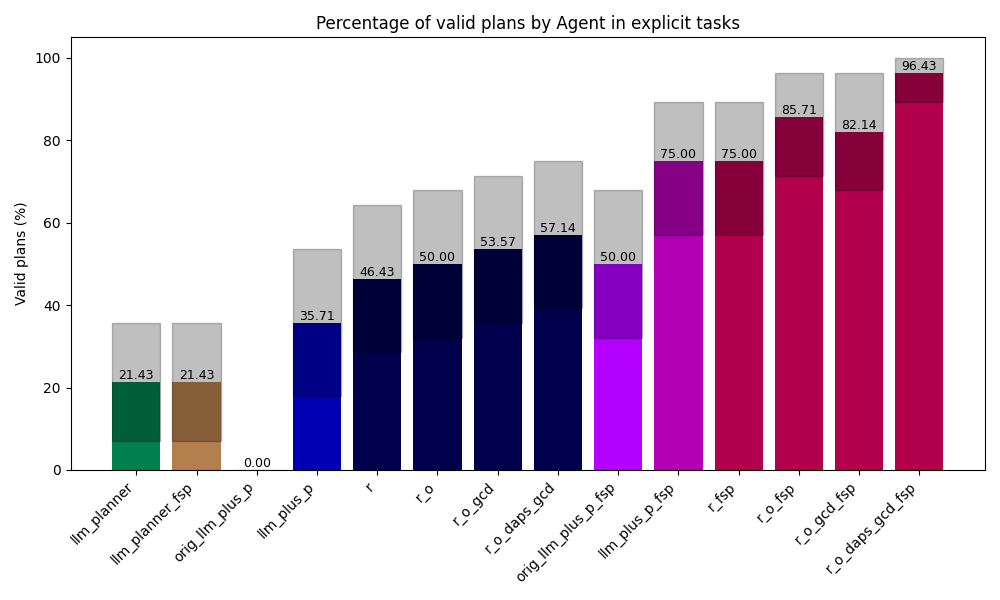
\includegraphics[width=0.7\textwidth]{Graphics/valid_plans_by_agent.png}
\caption{Porcentaje de planes válidos por agente en tareas con descripción completamente explícita.}
\label{fig:plans}
\end{figure}

A la izquierda se muestran los dos agentes planificadores reproducidos. A la derecha se presentan los agentes modeladores, organizados en dos grupos: los seis primeros no utilizan \textit{FSP}, mientras que los seis últimos sí lo hacen (indicados mediante barras en tonos más rojizos). Dentro de cada grupo, el orden corresponde a: agente original \textit{LLM+P}, reimplementación estructurada, y variantes con módulos adicionales. En todos los casos se sombrea el intervalo de confianza (IC) del 95\,\%.

Como se aprecia en la figura, ambos agentes planificadores generan planes válidos únicamente en el 21.43\,\% (IC: [7.14\,\%, 35.71\,\%]) de los problemas evaluados, es decir, 6 soluciones correctas. En cambio, todos los agentes modeladores ---con excepción de \texttt{orig\_llm\_plus\_p}--- superan ampliamente este resultado. Además, se observa una mejora progresiva en la métrica con la incorporación de los módulos propuestos. El agente que incluye todos los componentes alcanza el mejor desempeño, con una tasa de validez del 96.43\,\% (IC: [89.29\,\%, 100.00\,\%]), fallando solo en uno de los 28 problemas.

Estos resultados evidencian la complejidad del \textit{benchmark} Planetarium, que representa un reto considerable para agentes planificadores directos, y refuerzan la superioridad del enfoque basado en modelado explícito. Asimismo, proporcionan evidencia empírica del impacto positivo de los módulos de mejora propuestos, como antesala a los resultados globales que se presentan a continuación.

\section{Resultados generales}

En esta sección se presentan los resultados obtenidos por los distintos agentes modeladores evaluados sobre los 70 problemas del conjunto de prueba estratificado del \textit{benchmark Planetarium}, distribuidos en tres dominios: \textit{Blocksworld} (16 problemas), \textit{Gripper} (27 problemas) y \textit{Floor-Tile} (27 problemas). 

Se comparan 12 variantes de agentes: los agentes originales de \textit{LLM+P}, sus reimplementaciones estructuradas, y múltiples versiones incrementales mejoradas con los módulos propuestos en esta tesis. Las métricas consideradas incluyen: tasa de modelos con objetos correctamente identificados (\textit{Correct Objects count}), tasa de sintaxis válida (\textit{Parseable}), tasa de solubilidad (\textit{Solvable}) y tasa de problemas completamente correctos (\textit{Correct}). Cada métrica se expresa como porcentaje del total de problemas evaluados. Todos los intervalos de confianza (IC) presentados son del 95\,\%.

\subsection*{Tabla comparativa de métricas}

\begin{table}[H]
\centering
\label{tab:resultados_agentes}
\begin{tabular}{lcccc}
\toprule
\textbf{Agente} & \textbf{COC (\%)} & \textbf{Parseable (\%)} & \textbf{Solvable (\%)} & \textbf{Correct (\%)} \\
\midrule
\texttt{orig\_llm\_plus\_p} & \textcolor{red}{32.86} & \textcolor{red}{34.29} & \textcolor{red}{0.00} & \textcolor{red}{0.00} \\
\texttt{llm\_plus\_p} & 62.86 & \underline{87.14} & 54.29 & 22.86 \\
\texttt{r} & 62.86 & 82.86 & 62.86 & 30.00 \\
\texttt{r\_o} & \underline{95.71} & 84.29 & \underline{78.57} & \underline{42.86} \\
\texttt{r\_o\_gcd} & \textcolor{green!60!black}{98.57} & \underline{87.14} & 77.14 & \textcolor{green!60!black}{44.29} \\
\texttt{r\_o\_daps\_gcd} & 92.86 & \textcolor{green!60!black}{97.14} & \textcolor{green!60!black}{85.71} & 41.43 \\
\midrule
\texttt{orig\_llm\_plus\_p\_fsp} & \textbf{\textcolor{green!60!black}{100.00}} & \textcolor{red}{80.00} & \textcolor{red}{62.86} & \textcolor{red}{47.14} \\
\texttt{llm\_plus\_p\_fsp} & \textbf{\textcolor{green!60!black}{100.00}} & 87.14 & 82.86 & 57.14 \\
\texttt{r\_fsp} & \textbf{\textcolor{green!60!black}{100.00}} & 90.00 & 87.14 & 72.86 \\
\texttt{r\_o\_fsp} & \textbf{\textcolor{green!60!black}{100.00}} & 91.43 & \underline{88.57} & \underline{75.71} \\
\texttt{r\_o\_gcd\_fsp} & \textbf{\textcolor{green!60!black}{100.00}} & \underline{92.86} & \underline{88.57} & 67.14 \\
\texttt{r\_o\_daps\_gcd\_fsp} & \textbf{\textcolor{green!60!black}{100.00}} & \textbf{\textcolor{green!60!black}{100.00}} & \textbf{\textcolor{green!60!black}{94.29}} & \textbf{\textcolor{green!60!black}{81.43}} \\
\bottomrule
\end{tabular}
\caption{Resultados comparativos por agente modelador}
\end{table}

En la tabla anterior, los valores en \textcolor{green!60!black}{verde} indican el mejor resultado por métrica dentro de cada grupo (\textit{Zero-Shot} arriba y \textit{One-Shot} abajo), los \underline{subrayados} corresponden al segundo mejor valor, y los \textcolor{red}{rojos} representan el peor desempeño observado. En la tabla siguiente, de estas evaluaciones se destacan de igual manera los intervalos de confianza al 95\%.

\begin{table}[ht]
\centering
\small
\begin{tabular}{lcccc}
\toprule
\textbf{Agente} & \textbf{COC IC (\%)} & \textbf{Parseable IC (\%)} & \textbf{Solvable IC (\%)} & \textbf{Correct IC (\%)} \\
\midrule
\texttt{orig\_llm\_plus\_p} & \textcolor{red!70!black}{[22.86, 44.29]} & \textcolor{red!70!black}{[22.86, 45.71]} & \textcolor{red!70!black}{[0.00, 0.00]} & \textcolor{red!70!black}{[0.00, 0.00]} \\
\texttt{llm\_plus\_p} & [51.43, 74.29] & \underline{[78.57, 94.29]} & [42.86, 65.71] & [12.86, 32.86] \\
\texttt{r} & [51.43, 74.29] & [74.29, 91.43] & [51.43, 74.29] & [20.00, 41.43] \\
\texttt{r\_o} & \underline{[90.00, 100.00]} & [75.71, 92.86] & \underline{[68.57, 87.14]} & \underline{[31.43, 54.29]} \\
\texttt{r\_o\_gcd} & \textcolor{green!60!black}{[95.71, 100.00]} & \underline{[78.57, 94.29]} & [67.14, 87.14] & \textcolor{green!60!black}{[32.86, 55.71]} \\
\texttt{r\_o\_daps\_gcd} & [85.71, 98.57] & \textcolor{green!60!black}{[92.86, 100.00]} & \textcolor{green!60!black}{[77.14, 92.86]} & [30.00, 52.86] \\
\midrule
\texttt{orig\_llm\_plus\_p\_fsp} & \textbf{\textcolor{green!60!black}{[100.00, 100.00]}} & \textcolor{red!70!black}{[70.00, 88.57]} & \textcolor{red!70!black}{[51.43, 74.29]} & \textcolor{red!70!black}{[35.71, 58.57]} \\
\texttt{llm\_plus\_p\_fsp} & \textbf{\textcolor{green!60!black}{[100.00, 100.00]}} & [78.57, 94.29] & [74.29, 91.43] & [45.71, 68.57] \\
\texttt{r\_fsp} & \textbf{\textcolor{green!60!black}{[100.00, 100.00]}} & [82.86, 97.14] & [78.57, 94.29] & [61.43, 82.86] \\
\texttt{r\_o\_fsp} & \textbf{\textcolor{green!60!black}{[100.00, 100.00]}} & [84.29, 97.14] & \underline{[80.00, 95.71]} & \underline{[65.71, 85.71]} \\
\texttt{r\_o\_gcd\_fsp} & \textbf{\textcolor{green!60!black}{[100.00, 100.00]}} & \underline{[85.71, 98.57]} & \underline{[80.00, 95.71]} & [55.71, 78.57] \\
\texttt{r\_o\_daps\_gcd\_fsp} & \textbf{\textcolor{green!60!black}{[100.00, 100.00]}} & \textbf{\textcolor{green!60!black}{[100.00, 100.00]}} & \textbf{\textcolor{green!60!black}{[88.57, 98.57]}} & \textbf{\textcolor{green!60!black}{[71.43, 90.00]}} \\
\bottomrule
\end{tabular}
\caption{Intervalos de confianza al 95\% para cada métrica por agente.}
\label{tab:bootstrap_ic_agentes}
\end{table}


\subsection*{Gráficas comparativas}

\begin{figure}[H]
\centering
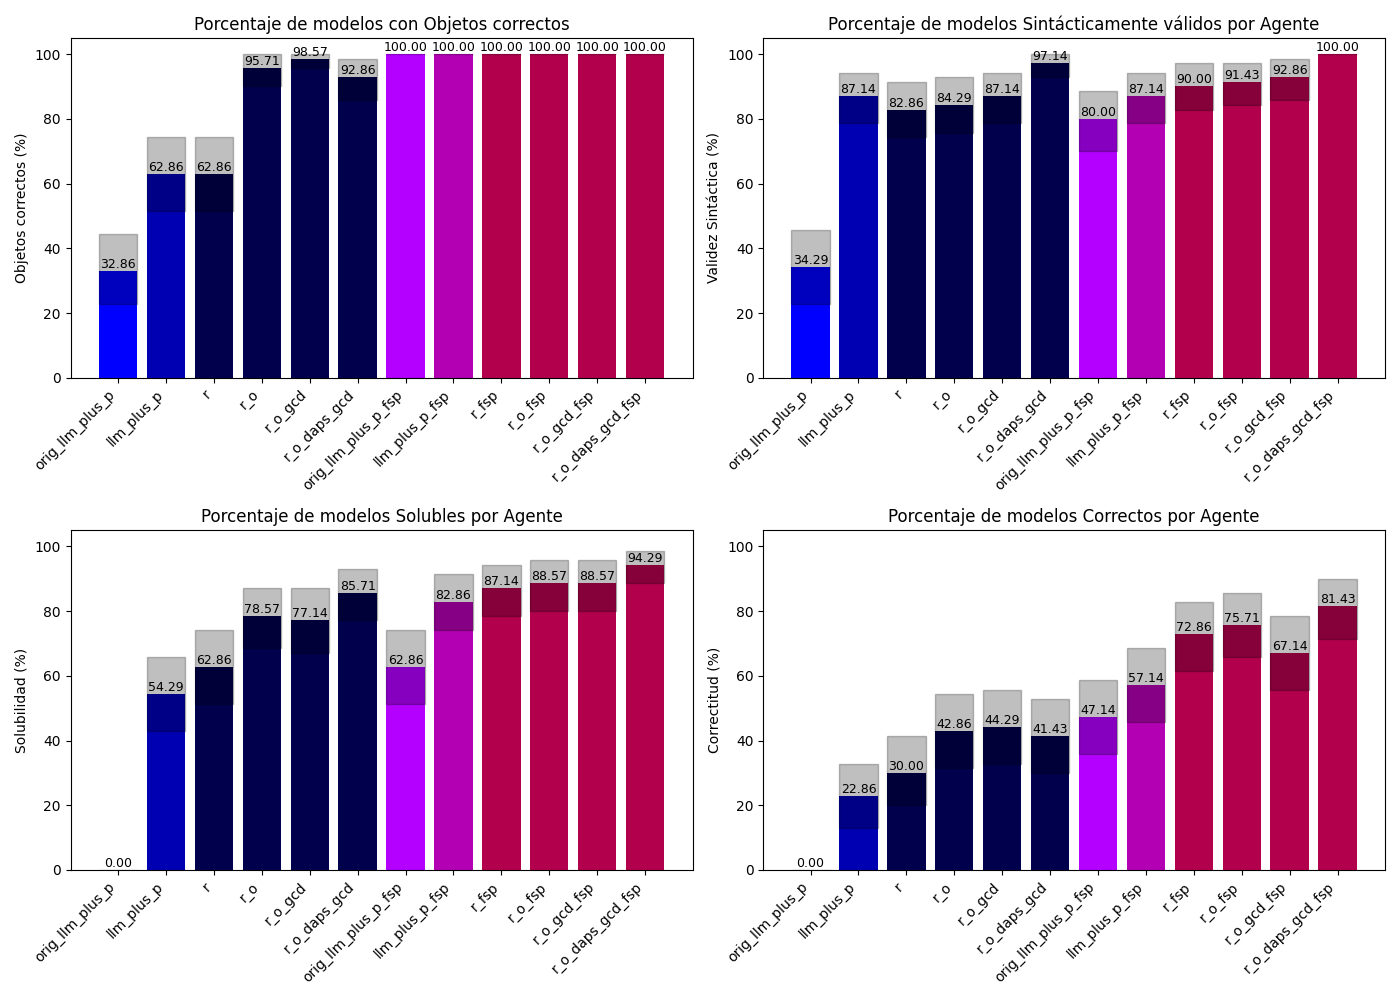
\includegraphics[width=0.8\textwidth]{Graphics/metrics_grid.png}
\caption{Métricas calculadas por agente}
\label{fig:objects}
\end{figure}

Estas gráficas de barras ilustran visualmente la evolución del desempeño de los agentes en cada una de las métricas clave. Los agentes se agrupan en dos bloques: los seis primeros no utilizan \textit{Few-Shot Prompting (FSP)}, mientras que los seis últimos sí lo hacen (indicados con barras en tonos más rojizos). En cada grupo, el orden de aparición sigue el patrón: agente original de \textit{LLM+P}, reimplementación estructurada, y variantes con módulos adicionales.

\subsection{Impacto del Razonamiento Estructurado}

El razonamiento estructurado fue incorporado como una fase previa y separada a la generación del modelo \textit{PDDL}, con el objetivo de descomponer semánticamente el problema y mejorar la calidad del modelado automático. Esta etapa adicional fue diseñada para inducir al \textit{LLM} a procesar explícitamente los objetos, el estado inicial y el estado objetivo antes de generar la solución final.

El impacto de este componente puede analizarse con claridad a partir de comparaciones directas entre agentes que difieren únicamente en la presencia del razonamiento. Por ejemplo, al comparar \texttt{llm\_plus\_p} con \texttt{r}, se observa una mejora en la proporción de modelos solubles, que aumenta de 54.29\,\% (IC: [42.86\,\%, 65.71\,\%]) a 62.86\,\% (IC: [51.43\,\%, 74.29\,\%]), así como en la proporción de problemas \textit{correctos}, que pasa de 22.86\,\% (IC: [12.86\,\%, 32.86\,\%]) a 30.00\,\% (IC: [20.00\,\%, 41.43\,\%]). Aunque los intervalos de confianza se superponen, la diferencia observada indica un efecto positivo consistente del componente, atribuible al cambio en la estrategia cognitiva del agente.

La comparación en presencia de \textit{Few-Shot Prompting (FSP)} ofrece aún mayor contraste. Al comparar \texttt{llm\_plus\_p\_fsp} con \texttt{r\_fsp}, se aprecia un aumento en la métrica de solubilidad de 82.86\,\% (IC: [74.29\,\%, 91.43\,\%]) a 87.14\,\% (IC: [78.57\,\%, 94.29\,\%]), y en la de \textit{correctitud completa} de 57.14\,\% (IC: [45.71\,\%, 68.57\,\%]) a 72.86\,\% (IC: [61.43\,\%, 82.86\,\%]). Esta diferencia es significativa tanto en magnitud como en intervalo de confianza, y puede explicarse por el hecho de que los ejemplos de \textit{FSP} fueron cuidadosamente diseñados para mostrar razonamientos y desambiguaciones correctas, lo que actúa como una guía concreta para que el \textit{LLM} aprenda cómo estructurar sus propias inferencias sobre tareas de planificación.

Los beneficios del razonamiento no se extienden a las métricas de \textit{objetos correctos} y \textit{modelo con sintaxis válida}, pero no tiene un efecto negativo palpable. Por ejemplo, entre \texttt{llm\_plus\_p} y \texttt{r}, la proporción de objetos correctamente identificados se mantiene constante en 62.86\,\% (IC: [51.43\,\%, 74.29\,\%]), lo cual sugiere que este componente no deteriora la precisión de este aspecto, mientras que la validez sintáctica se mantiene elevada (de 87.14\,\% (IC: [78.57\,\%, 94.29\,\%]) a 82.86\,\% (IC: [74.29\,\%, 91.43\,\%])), aunque con una ligera caída en la media. Estas fluctuaciones pueden deberse a alucinaciones, que en ausencia de ejemplos de \textit{FSP} y razonamiento ineficiente pueden acentuarse. Más aún, se observa que la validez sintáctica aumenta ligeramente en el par de agentes \textit{One-Shot}, de 87.14\,\% (IC: [78.57\,\%, 94.29\,\%]) a 90.00\,\% (IC: [82.86\,\%, 97.14\,\%]). Sin embargo, estos resultados no son concluyentes y no comprometen la interpretación general.

Cabe destacar que, debido al diseño incremental del sistema, los resultados de los agentes más avanzados (como \texttt{r\_o\_gcd} o \texttt{r\_o\_daps\_gcd}) reflejan interacciones acumulativas entre múltiples componentes. Por tanto, el impacto aislado del razonamiento estructurado debe analizarse principalmente en los pares donde es el único cambio introducido. Aun así, su presencia constante en los agentes de mayor rendimiento (tanto con como sin \textit{FSP}) sugiere que su efecto es no solo positivo, sino posiblemente sinérgico con otros módulos.

Estos resultados empíricos se alinean con hallazgos previos en la literatura, que indican que la inclusión de pasos intermedios de razonamiento mejora las capacidades de los \textit{LLMs} en tareas complejas \parencite{wei2022chain, yao2023tree}. En particular, trabajos como \textit{ReAct} \parencite{yao2023react} han demostrado que combinar razonamiento textual con ejecución no solo mejora la calidad de las salidas, sino que también aumenta la interpretabilidad del proceso. Los resultados obtenidos en esta tesis refuerzan dicha hipótesis, mostrando que una etapa explícita de razonamiento puede traducirse en mejoras cuantificables en desempeño y robustez del agente modelador.

\subsection{Impacto de la Extracción de Objetos}

La Extracción de Objetos se incorporó como una etapa estructurada y especializada con el objetivo de mejorar la precisión semántica y sintáctica del modelo \textit{PDDL} generado. Al separar explícitamente la identificación de objetos relevantes del resto del proceso, se busca garantizar la integridad del conjunto de elementos que participan en el problema de planificación. Esta fase se implementó posterior al razonamiento (cuando está activo), permitiendo heredar y organizar las inferencias previas, y su salida se genera en un formato \textit{JSON} que facilita su uso posterior en componentes como la generación asistida por gramática (\textit{GCD}).

Desde el punto de vista empírico, el impacto de este componente puede observarse de forma clara al comparar agentes que difieren únicamente en la presencia de esta fase. El caso más representativo es el contraste entre \texttt{r} y \texttt{r\_o}, donde se mantiene el razonamiento estructurado y se añade únicamente la extracción de objetos. En esta comparación, la proporción de objetos correctamente identificados aumenta de 62.86\,\% (IC: [51.43\,\%, 74.29\,\%]) a 95.71\,\% (IC: [90.00\,\%, 100.00\,\%]), lo cual representa una mejora sustancial en el componente más directamente afectado por esta fase.

Además, esta mejora en la identificación de objetos se traduce en ganancias indirectas en otras métricas. La validez sintáctica se mantiene estable, con un ligero aumento de 82.86\,\% (IC: [74.29\,\%, 91.43\,\%]) a 84.29\,\% (IC: [75.71\,\%, 92.86\,\%]). La solubilidad mejora sustancialmente, de 62.86\,\% (IC: [51.43\,\%, 74.29\,\%]) a 78.57\,\% (IC: [68.57\,\%, 87.14\,\%]). En correctitud total, \texttt{r} alcanza 30.00\,\% (IC: [20.00\,\%, 41.43\,\%]), mientras que \texttt{r\_o} sube a 42.86\,\% (IC: [31.43\,\%, 54.29\,\%]). Esto sugiere que la correcta extracción y estructuración de objetos permite al modelo generar instancias más completas y coherentes, impactando positivamente tanto en la validez sintáctica como semántica.

Un patrón similar se repite en los agentes que incorporan \textit{FSP}. Comparando \texttt{r\_fsp} y \texttt{r\_o\_fsp}, se observa una mejora en solubilidad de 87.14\,\% (IC: [78.57\,\%, 94.29\,\%]) a 88.57\,\% (IC: [80.00\,\%, 95.71\,\%]), así como una ganancia en correctitud total de 72.86\,\% (IC: [61.43\,\%, 82.86\,\%]) a 75.71\,\% (IC: [65.71\,\%, 85.71\,\%]). Aunque estas diferencias son más sutiles, reflejan una consolidación de los beneficios observados en el grupo sin \textit{FSP}.

Estas observaciones refuerzan la utilidad de una fase de extracción dedicada, especialmente en contextos donde la ambigüedad o la omisión de objetos puede deteriorar gravemente la calidad del modelo generado. Al permitir una representación explícita, detallada y consistente de los objetos del dominio, este componente actúa como un estabilizador semántico clave que fortalece las fases posteriores del \textit{pipeline} de modelado.

Finalmente, es importante señalar que este módulo facilita no solo la calidad de los modelos, sino también su inspeccionabilidad y adaptabilidad. Su diseño como fase independiente y estructurada habilita un nivel adicional de trazabilidad que puede ser aprovechado tanto para depuración como para transferencia de conocimiento entre tareas similares, especialmente cuando se combina con componentes como \textit{GCD} o reflexión estructurada. Permite, más aún, la aplicación de la modalidad \textit{DAPS} concebida de \textit{GCD}, al restringir la salida del modelo a una gramática específica al problema a modelar, limitando los argumentos utilizados en las proposiciones a aquellos objetos extraídos en esta fase, con correcto tipado si lo presentan.

\subsection{Impacto de \textit{Grammar-Constrained Decoding (GCD)} y su variante \textit{Domain-and Problem-Specific (DAPS)}}

El módulo de \textit{GCD} fue introducido con el objetivo de garantizar la validez sintáctica de los modelos \textit{PDDL} generados, mediante la incorporación de una gramática explícita sobre la estructura del lenguaje. Como punto de partida, se utilizó una gramática en formato \textit{GBNF} que captura la sintaxis del subconjunto de \textit{PDDL} empleado, incluyendo soporte para dominios tipados y la estructura general de \textit{STRIPS}. Esta gramática permite restringir la generación a secuencias sintácticamente válidas, pero no impone restricciones semánticas específicas al dominio o problema en cuestión.

Para superar estas limitaciones, se introdujo una variante más estricta denominada \textit{Domain-and Problem-Specific (DAPS)}, la cual incorpora de forma dinámica los predicados, tipos y objetos específicos del problema en curso. En particular, se especializa la producción de fórmulas atómicas dentro de las secciones \texttt{:init} y \texttt{:goal}, de modo que solo se aceptan predicados válidos del dominio, con aridad exacta y argumentos seleccionados exclusivamente del conjunto de objetos declarados. Esto impide que el modelo produzca contenido fuera del esquema válido, como razonamientos embebidos o correcciones autorreferenciales dentro de estructuras que requieren literalidad.

Un ejemplo de este comportamiento problemático puede verse en la producción básica de fórmulas atómicas sin restricciones específicas:

\begin{verbatim}
atomicFormula ::= "(" name (ws object)* ")"
\end{verbatim}

Esta definición permite que casi cualquier secuencia de texto sea interpretada como el nombre de un predicado o un argumento, lo que en la práctica genera errores de sintaxis, especialmente cuando el \textit{LLM} introduce razonamientos o comentarios no deseados dentro de las proposiciones. En contraste, en la modalidad \textit{DAPS} se sustituye esta producción por una versión especializada que considera únicamente combinaciones válidas y completas de predicado y argumentos.

En términos empíricos, el impacto de \textit{GCD} puede observarse en el paso de \texttt{r\_o} a \texttt{r\_o\_gcd}, donde se mantiene el razonamiento y la extracción de objetos, pero se añade el uso de la gramática general. La validez sintáctica mejora de 84.29\,\% (IC: [75.71\,\%, 92.86\,\%]) a 87.14\,\% (IC: [78.57\,\%, 94.29\,\%]), lo cual muestra una ganancia modesta, posiblemente limitada por las desviaciones mencionadas. Estas también afectan la solubilidad, donde se observa un ligero descenso, de 78.57\,\% (IC: [68.57\,\%, 87.14\,\%]) a 77.14\,\% (IC: [67.14\,\%, 87.14\,\%]), aunque no es estadísticamente significativo considerando la intersección casi total de los intervalos de confianza. La correctitud total sube levemente de 42.86\,\% (IC: [31.43\,\%, 54.29\,\%]) a 44.29\,\% (IC: [32.86\,\%, 55.71\,\%]).

Sin embargo, la modalidad \textit{DAPS} muestra una mejora mucho más marcada. En \texttt{r\_o\_daps\_gcd}, se observa que la validez sintáctica alcanza el 97.14\,\% (IC: [92.86\,\%, 100.00\,\%]). También se reporta un aumento significativo en solubilidad, a 85.71\,\% (IC: [77.14\,\%, 92.86\,\%]), aunque esta mejora no se observa en la correctitud, posiblemente por la ausencia en el contexto de buenos ejemplos de razonamiento estructurado. Estos resultados respaldan empíricamente la hipótesis de que una gramática altamente especializada aporta grandes beneficios en la validez sintáctica de los modelos.

Este efecto se ve reforzado cuando se analiza la interacción con \textit{Few-Shot Prompting (FSP)}. En el caso del agente \texttt{r\_o\_fsp}, que ya alcanza valores altos en todas las métricas, se obtiene una validez sintáctica de 91.43\,\% (IC: [84.29\,\%, 97.14\,\%]), una \textit{solubilidad} de 88.57\,\% (IC: [80.00\,\%, 95.71\,\%]) y una \textit{correctitud total} de 75.71\,\% (IC: [65.71\,\%, 85.71\,\%]). Al incorporar la gramática general mediante \texttt{GCD} en \texttt{r\_o\_gcd\_fsp}, la validez sintáctica mejora levemente a 92.86\,\% (IC: [85.71\,\%, 98.57\,\%]), y la solubilidad se mantiene constante, aunque la correctitud total disminuye a 67.14\,\% (IC: [55.71\,\%, 78.57\,\%]), probablemente debido a las desviaciones observadas por control gramatical y semántico incompleto. Finalmente, al incorporar la modalidad \textit{DAPS} en \texttt{r\_o\_daps\_gcd\_fsp}, se logra validez sintáctica perfecta (100\,\%, IC: [100\,\%, 100\,\%]), una solubilidad de 94.29\,\% (IC: [88.57\,\%, 98.57\,\%]) y una correctitud total de 81.43\,\% (IC: [71.43\,\%, 90.00\,\%]), lo cual representa el mejor desempeño alcanzado por cualquier agente evaluado en todas las métricas, con una diferencia marcada.

Cabe señalar que, pese a la formalización gramatical, la modalidad \textit{GCD} no garantiza validez sintáctica perfecta por sí sola. Esto se debe a que las gramáticas generales no impiden por completo que el \textit{LLM} inserte contenido erróneo o se desvíe del formato literal requerido, como ocurre al generar proposiciones en \texttt{:init} y \texttt{:goal}. Solo mediante la especialización del conjunto de producciones a través de \textit{DAPS} se evita completamente este comportamiento.

Estos hallazgos empíricos respaldan las observaciones de trabajos previos como \parencite{loula2025syntactic}, que demostraban el potencial de \textit{GCD} para mejorar la coherencia sintáctica en dominios acotados. Sin embargo, la evaluación presentada en esta tesis extiende significativamente dicho análisis al considerar la generación completa de modelos \textit{PDDL} a partir de descripciones en lenguaje natural y una evaluación exhaustiva sobre un subconjunto estratificado de problemas más representativo del \textit{benchmark Planetarium}. Además, se introduce y valida empíricamente un refinamiento fundamental: la especialización semántica de la gramática con base en el dominio y problema, lo cual constituye un avance práctico y conceptual en el uso de \textit{GCD} para modelado automático en planificación.

\subsection{Un salto cualitativo sobre los \textit{baselines} existentes}

Para ilustrar la magnitud del avance logrado por la variante \texttt{r\_o\_daps\_gcd\_fsp}, es fundamental contrastarla con los \textit{baselines} \texttt{orig\_llm\_plus\_p\_fsp} y \texttt{llm\_plus\_p\_fsp}. En validez sintáctica, los valores de 80.00\,\% y 87.14\,\% alcanzados por los respectivos \textit{baselines} son completamente superados: \texttt{r\_o\_daps\_gcd\_fsp} logra una cobertura total del 100\,\%, cerrando el 100\,\% del margen restante en ambos casos. 

En solubilidad, la mejora es igualmente destacable. \texttt{orig\_llm\_plus\_p\_fsp} alcanzaba 62.86\,\%, quedando un 37.14\,\% por recorrer; \texttt{r\_o\_daps\_gcd\_fsp} logra 94.29\,\%, salvando 31.43 puntos, lo que equivale a un 84.63\,\% de ese margen. Similarmente, frente al 82.86\,\% de \texttt{llm\_plus\_p\_fsp}, que dejaba 17.14\,\% por cubrir, \texttt{r\_o\_daps\_gcd\_fsp} salva 11.43 puntos, un 66.67\,\% del margen de mejora.

La diferencia es aún más relevante en \textit{correctitud total}, la métrica más exigente e importante. En ella \texttt{orig\_llm\_plus\_p\_fsp} obtenía 47.14\,\% (quedando un 52.86\,\% restante), y \texttt{r\_o\_daps\_gcd\_fsp} alcanza 81.43\,\%, cubriendo 34.29 puntos, un 64.86\,\% del espacio disponible. Frente a \texttt{llm\_plus\_p\_fsp} (57.14\,\%), que dejaba 42.86\,\% por salvar, la misma variante logra cubrir 24.29 puntos, es decir un 56.67\,\% de dicho faltante. Dicho de otro modo, más de la mitad de lo que los agentes anteriores no lograban modelar correctamente, es resuelto por la variante que aplica todas las mejoras propuestas.

Estos cálculos muestran que, más allá de la diferencia absoluta en puntos porcentuales, la combinación de \textit{GCD} especializada (\textit{DAPS}) con \textit{FSP} manual, mecanismos de \textit{extracción de objetos} consistentes, y el uso explícito de \textit{razonamiento estructurado}, proporciona una mejora \textbf{proporcionalmente muy significativa} sobre lo que faltaba en los \textit{baselines}. Estos resultados demuestran empíricamente el potencial de los componentes propuestos actuando en conjunto para cerrar brechas que los enfoques anteriores apenas lograban mitigar.

\definecolor{verde}{HTML}{008000} % Define el color verde
\definecolor{rojo}{HTML}{FF0000} % Define el color rojo

\section{Entrenamiento del agente modelador experiencial}

Se llevó a cabo el entrenamiento propuesto del agente modelador experiencial sobre el subconjunto seleccionado de 100 problemas, 50 del dominio \textit{Blocksworld} y 50 del dominio \textit{Gripper}. El agente implementó la configuración \texttt{r\_o\_daps\_gcd\_fsp}, incorporando los módulos de Razonamiento Estructurado, Extracción de Objetos, \textit{GCD DAPS} y un ejemplo \textit{FSP} definido manualmente, representando así la mejor versión evaluada en iteraciones anteriores. Además, se integró el mecanismo de reintentos, que permitía al agente iterar hasta tres veces sobre cada problema, guiado por \textit{feedback} automático y autorreflexión para mejorar su rendimiento. El agente resultante será denominado \texttt{exp} por simplicidad.

La tabla que se presenta a continuación resume los resultados de este proceso de entrenamiento. Cada fila corresponde a una configuración particular de resultados a través de los tres intentos permitidos por problema. Para cada intento, se registran tres las métricas definidas anteriormente: \textit{Parseable} ($\mathcal{P}$), \textit{Solvable} ($\mathcal{S}$) y \textit{Correct} ($\mathcal{C}$). Una \textcolor{verde}{\textbf{V}} representa un resultado positivo, mientras que una \textcolor{rojo}{\textbf{F}} indica un resultado negativo para esa métrica en ese intento. El índice numérico en cada métrica indica el intento (ej., $\mathcal{P}_1$ corresponde a la validez sintáctica en el primer intento). La última columna, ``Número de Problemas'', indica la cantidad de problemas que determinaron esa secuencia específica de resultados a lo largo de los intentos del agente.

\begin{table}[h!]
    \centering
    \caption{Resultados del Agente en Problemas de Planificación}
    \begin{tabular}{ccc@{\hspace{2em}}ccc@{\hspace{2em}}ccc@{\hspace{2em}}c}
        \toprule
        \multicolumn{3}{c}{\textbf{Intento 1}} & \multicolumn{3}{c}{\textbf{Intento 2}} & \multicolumn{3}{c}{\textbf{Intento 3}} & \textbf{Número de Problemas} \\
        \cmidrule(lr){1-3} \cmidrule(lr){4-6} \cmidrule(lr){7-9}
        $\mathcal{P}_1$ & $\mathcal{S}_1$ & $\mathcal{C}_1$ & $\mathcal{P}_2$ & $\mathcal{S}_2$ & $\mathcal{C}_2$ & $\mathcal{P}_3$ & $\mathcal{S}_3$ & $\mathcal{C}_3$ & \\
        \midrule
        \textcolor{verde}{\textbf{V}} & \textcolor{verde}{\textbf{V}} & \textcolor{verde}{\textbf{V}} & - & - & - & - & - & - & 87 \\
        \textcolor{verde}{\textbf{V}} & \textcolor{verde}{\textbf{V}} & \textcolor{rojo}{\textbf{F}} & \textcolor{verde}{\textbf{V}} & \textcolor{verde}{\textbf{V}} & \textcolor{verde}{\textbf{V}} & - & - & - & 2 \\
        \textcolor{verde}{\textbf{V}} & \textcolor{verde}{\textbf{V}} & \textcolor{rojo}{\textbf{F}} & \textcolor{verde}{\textbf{V}} & \textcolor{verde}{\textbf{V}} & \textcolor{rojo}{\textbf{F}} & \textcolor{verde}{\textbf{V}} & \textcolor{verde}{\textbf{V}} & \textcolor{verde}{\textbf{V}} & 1 \\
        \textcolor{verde}{\textbf{V}} & \textcolor{verde}{\textbf{V}} & \textcolor{rojo}{\textbf{F}} & \textcolor{verde}{\textbf{V}} & \textcolor{verde}{\textbf{V}} & \textcolor{rojo}{\textbf{F}} & \textcolor{verde}{\textbf{V}} & \textcolor{verde}{\textbf{V}} & \textcolor{rojo}{\textbf{F}} & 2 \\
        \textcolor{verde}{\textbf{V}} & \textcolor{rojo}{\textbf{F}} & \textcolor{rojo}{\textbf{F}} & \textcolor{verde}{\textbf{V}} & \textcolor{verde}{\textbf{V}} & \textcolor{verde}{\textbf{V}} & - & - & - & 4 \\
        \textcolor{verde}{\textbf{V}} & \textcolor{rojo}{\textbf{F}} & \textcolor{rojo}{\textbf{F}} & \textcolor{verde}{\textbf{V}} & \textcolor{rojo}{\textbf{F}} & \textcolor{rojo}{\textbf{F}} & \textcolor{verde}{\textbf{V}} & \textcolor{verde}{\textbf{V}} & \textcolor{verde}{\textbf{V}} & 1 \\
        \textcolor{verde}{\textbf{V}} & \textcolor{rojo}{\textbf{F}} & \textcolor{rojo}{\textbf{F}} & \textcolor{verde}{\textbf{V}} & \textcolor{rojo}{\textbf{F}} & \textcolor{rojo}{\textbf{F}} & \textcolor{verde}{\textbf{V}} & \textcolor{rojo}{\textbf{F}} & \textcolor{rojo}{\textbf{F}} & 1 \\
        \textcolor{rojo}{\textbf{F}} & \textcolor{rojo}{\textbf{F}} & \textcolor{rojo}{\textbf{F}} & \textcolor{verde}{\textbf{V}} & \textcolor{verde}{\textbf{V}} & \textcolor{verde}{\textbf{V}} & - & - & - & 1 \\
        \textcolor{rojo}{\textbf{F}} & \textcolor{rojo}{\textbf{F}} & \textcolor{rojo}{\textbf{F}} & \textcolor{verde}{\textbf{V}} & \textcolor{rojo}{\textbf{F}} & \textcolor{rojo}{\textbf{F}} & \textcolor{verde}{\textbf{V}} & \textcolor{verde}{\textbf{V}} & \textcolor{verde}{\textbf{V}} & 1 \\
        \bottomrule
    \end{tabular}
    \label{tab:entrenamiento}
\end{table}

Los resultados revelan una alta tasa de éxito en el primer intento, con 87 problemas siendo resueltos correctamente de inmediato. Sin embargo, la inclusión del mecanismo de reintentos demostró ser crucial para mejorar el rendimiento general. Si bien algunos problemas presentaron dificultades persistentes a lo largo de los tres intentos, la autorreflexión y el \textit{feedback} automático permitieron al agente corregir errores y alcanzar soluciones completamente correctas en intentos posteriores para 10 de los 13 problemas inicialmente fallidos. De los 3 problemas cuyo modelado no fue correcto en ninguno de los intentos, 2 resultaron solubles. Contando únicamente los primeros intentos por cada problema, se alcanzaban tasas de validez sintáctica de 98 \% (debido a truncamientos de la salida del \textit{LLM}), 92 \% de solubilidad y 87 \% de correctitud. Finalmente, con la integración de los reintentos, el agente \texttt{exp} alcanzó en el entrenamiento una validez sintáctica del 100 \%, solubilidad del 99 \%, y 97 \% de correctitud. Este análisis sugiere que la combinación de capacidades de modelado robustas con mecanismos adaptativos de auto-mejora contribuye significativamente a la capacidad del agente para abordar una amplia gama de desafíos de planificación.

\section{Aplicación de reintentos, \textit{feedback} y reflexión a la evaluación}

El agente \texttt{exp} aplicó la política de reintentos definida anteriormente a los problemas modelados incorrectamente por el agente \texttt{r\_o\_daps\_gcd\_fsp}, sobre el subconjunto de evaluación. Las salidas (razonamiento, objetos extraídos y \textit{PDDL} del problema) generados en su primer y único intento por tarea, y el \textit{feedback} construido automáticamente sobre este fallo, contribuyeron a un segundo intento que incluyó reflexión sobre la retroalimentación dada. De igual forma, se permitió un tercer intento apoyado en los resultados del segundo, si este era incorrecto.

La evaluación de \texttt{exp} se resume en la tabla siguiente:

\begin{table}[h!]
    \centering
    \caption{Resultados del Agente en el conjunto de Evaluación}
    \begin{tabular}{ccc@{\hspace{2em}}ccc@{\hspace{2em}}ccc@{\hspace{2em}}c}
        \toprule
        \multicolumn{3}{c}{\textbf{Intento 1}} & \multicolumn{3}{c}{\textbf{Intento 2}} & \multicolumn{3}{c}{\textbf{Intento 3}} & \textbf{Número de Problemas} \\
        \cmidrule(lr){1-3} \cmidrule(lr){4-6} \cmidrule(lr){7-9}
        $\mathcal{P}_1$ & $\mathcal{S}_1$ & $\mathcal{C}_1$ & $\mathcal{P}_2$ & $\mathcal{S}_2$ & $\mathcal{C}_2$ & $\mathcal{P}_3$ & $\mathcal{S}_3$ & $\mathcal{C}_3$ & \\
        \midrule
        \textcolor{verde}{\textbf{V}} & \textcolor{verde}{\textbf{V}} & \textcolor{verde}{\textbf{V}} & - & - & - & - & - & - & 57 \\
        \textcolor{verde}{\textbf{V}} & \textcolor{verde}{\textbf{V}} & \textcolor{rojo}{\textbf{F}} & \textcolor{verde}{\textbf{V}} & \textcolor{verde}{\textbf{V}} & \textcolor{rojo}{\textbf{F}} & \textcolor{verde}{\textbf{V}} & \textcolor{verde}{\textbf{V}} & \textcolor{rojo}{\textbf{F}} & 5 \\
        \textcolor{verde}{\textbf{V}} & \textcolor{verde}{\textbf{V}} & \textcolor{rojo}{\textbf{F}} & \textcolor{verde}{\textbf{V}} & \textcolor{verde}{\textbf{V}} & \textcolor{rojo}{\textbf{F}} & \textcolor{rojo}{\textbf{F}} & \textcolor{rojo}{\textbf{F}} & \textcolor{rojo}{\textbf{F}} & 2 \\
        \textcolor{verde}{\textbf{V}} & \textcolor{verde}{\textbf{V}} & \textcolor{rojo}{\textbf{F}} & \textcolor{verde}{\textbf{V}} & \textcolor{rojo}{\textbf{F}} & \textcolor{rojo}{\textbf{F}} & \textcolor{verde}{\textbf{V}} & \textcolor{verde}{\textbf{V}} & \textcolor{rojo}{\textbf{F}} & 1 \\
        \textcolor{verde}{\textbf{V}} & \textcolor{verde}{\textbf{V}} & \textcolor{rojo}{\textbf{F}} & \textcolor{rojo}{\textbf{F}} & \textcolor{rojo}{\textbf{F}} & \textcolor{rojo}{\textbf{F}} & \textcolor{verde}{\textbf{V}} & \textcolor{verde}{\textbf{V}} & \textcolor{rojo}{\textbf{F}} & 1 \\
        \textcolor{verde}{\textbf{V}} & \textcolor{rojo}{\textbf{F}} & \textcolor{rojo}{\textbf{F}} & \textcolor{verde}{\textbf{V}} & \textcolor{verde}{\textbf{V}} & \textcolor{rojo}{\textbf{F}} & \textcolor{verde}{\textbf{V}} & \textcolor{verde}{\textbf{V}} & \textcolor{verde}{\textbf{V}} & 2 \\
        \textcolor{verde}{\textbf{V}} & \textcolor{rojo}{\textbf{F}} & \textcolor{rojo}{\textbf{F}} & \textcolor{verde}{\textbf{V}} & \textcolor{verde}{\textbf{V}} & \textcolor{rojo}{\textbf{F}} & \textcolor{verde}{\textbf{V}} & \textcolor{rojo}{\textbf{F}} & \textcolor{rojo}{\textbf{F}} & 1 \\
        \textcolor{verde}{\textbf{V}} & \textcolor{rojo}{\textbf{F}} & \textcolor{rojo}{\textbf{F}} & \textcolor{verde}{\textbf{V}} & \textcolor{rojo}{\textbf{F}} & \textcolor{rojo}{\textbf{F}} & \textcolor{verde}{\textbf{V}} & \textcolor{rojo}{\textbf{F}} & \textcolor{rojo}{\textbf{F}} & 1 \\
        \bottomrule
    \end{tabular}
    \label{tab:eval_con_reintentos}
\end{table}

Los resultados obtenidos en la evaluación son menos alentadores que los del entrenamiento. En general, el agente con reflexión (\texttt{exp}) mostró dificultades para mejorar su desempeño, e incluso en algunos casos obtuvo resultados inferiores en reintentos. Esto podría atribuirse a la mayor complejidad inherente a los problemas no resueltos, que frecuentemente involucraban modelos \textit{PDDL} con un centenar de proposiciones. Los reintentos se caracterizaron por dos factores que afectaron negativamente al agente: un contexto mucho más extenso, influenciado por las salidas previas, y una reflexión propensa a alucinaciones. La degradación del rendimiento de los \textit{LLMs} con contextos extensos es un fenómeno bien documentado \parencite{li2024long}. Esta problemática se exacerbó en los problemas del dominio \textit{Floor-Tile}, ausente en el conjunto de entrenamiento anteriormente analizado. Este dominio requiere múltiples proposiciones para definir explícitamente la adyacencia entre celdas, utilizando predicados como \texttt{(up tileX tileY)} y \texttt{(right tileX tileY)}.  Con frecuencia, el agente alucinaba la existencia y necesidad de predicados similares como \texttt{left} y \texttt{down}. Aunque estos predicados no son permitidos por la restricción gramatical implementada con \textit{DAPS GCD}, su alucinación en la reflexión o razonamiento constituye ruido que dificulta el modelado correcto.

A pesar de estos resultados iniciales, el potencial de los mecanismos propuestos no debe descartarse. De los 13 problemas que el agente no logró modelar correctamente en el intento inicial de la etapa de evaluación, se corrigieron 2 gracias a los reintentos. La evaluación inicial ya mostraba resultados elevados, con un 100\,\% de validez sintáctica, un 94.29\,\% de solubilidad y un 81.43\,\% de correctitud, con dificultad de mejoría. Sin embargo, al considerar el mejor resultado obtenido en los reintentos para cada problema, estas métricas se incrementan a 100\,\%, 98.57\,\% y 84.29\,\%, respectivamente.

\section{Extracción de \textit{insights}}

La fase de extracción de \textit{insights}, posterior a la acumulación de experiencias durante el entrenamiento, se llevó a cabo de forma exploratoria. Sin embargo, los resultados iniciales no fueron del todo satisfactorios. Los \textit{insights} generados por el \textit{LLM}, actuando como agente extractor, tendían a ser vagos, genéricos o poco relevantes. En muchos casos, no lograban captar conocimiento concreto o útil del dominio que pudiera contribuir de forma significativa al modelado de nuevos problemas.

Además, las respuestas del modelo presentaban divagaciones extensas, con escasa alineación a las operaciones válidas del entorno, y sin un control efectivo sobre las restricciones sintácticas y semánticas de las acciones. Esto generó dificultades importantes para el análisis automático de las salidas, afectando la robustez del procesamiento posterior y provocando errores de ejecución en algunos casos. Estos comportamientos apuntan a posibles deficiencias en la ingeniería de \textit{prompts}, particularmente en su capacidad para guiar al modelo hacia la identificación de patrones estructurados y reutilizables de conocimiento relevante.

\section{Evaluación del agente experiencial con todos los módulos incluidos}

En la fase final de experimentación se evaluó el agente modelador completo, que integra todos los componentes diseñados en esta tesis para mejorar progresivamente los resultados. Este agente experiencial, reforzado con ejemplos derivados de experiencias anteriores, incorpora módulos de recuperación de ejemplos vía \textit{RAG} y conocimiento experto curado manualmente.

En concreto, se reutilizaron los ejemplos de \textit{FSP} aprendidos durante la fase de entrenamiento para los dominios \textit{Blocksworld} y \textit{Gripper}, recuperados automáticamente mediante \textit{RAG}. Para el dominio \textit{Floor-Tile}, sin instancias incluidas en el entrenamiento, se empleó el ejemplo construido manualmente.

Dado el rendimiento limitado observado en la extracción automática de \textit{insights}, se diseñó y empleó una base de \textit{Human Insights} (HI) creada manualmente. Esta decisión permite evaluar el impacto de integrar conocimiento estructurado y explícito, extraído por un experto humano, en lugar de depender exclusivamente de la inferencia del modelo, cuya mejora se delega a trabajo futuro.

El agente evaluado, denominado \texttt{exp\_rag\_hi}, combina así dos mecanismos de conocimiento experiencial: \textit{Retrieval-Augmented Generation} (RAG) y \textit{Human Insights} (HI). Los resultados obtenidos se presentan a continuación.

\begin{table}[H]
    \centering
    \caption{Resultados en el conjunto completo de evaluación}
    \begin{tabular}{ccc@{\hspace{2em}}ccc@{\hspace{2em}}ccc@{\hspace{2em}}c}
        \toprule
        \multicolumn{3}{c}{\textbf{Intento 1}} & \multicolumn{3}{c}{\textbf{Intento 2}} & \multicolumn{3}{c}{\textbf{Intento 3}} & \textbf{Número de Problemas} \\
        \cmidrule(lr){1-3} \cmidrule(lr){4-6} \cmidrule(lr){7-9}
        $\mathcal{P}_1$ & $\mathcal{S}_1$ & $\mathcal{C}_1$ & $\mathcal{P}_2$ & $\mathcal{S}_2$ & $\mathcal{C}_2$ & $\mathcal{P}_3$ & $\mathcal{S}_3$ & $\mathcal{C}_3$ & \\
        \midrule
        \textcolor{verde}{\textbf{V}} & \textcolor{verde}{\textbf{V}} & \textcolor{verde}{\textbf{V}} & - & - & - & - & - & - & 57 \\
        \textcolor{verde}{\textbf{V}} & \textcolor{verde}{\textbf{V}} & \textcolor{rojo}{\textbf{F}} & \textcolor{verde}{\textbf{V}} & \textcolor{verde}{\textbf{V}} & \textcolor{verde}{\textbf{V}} & - & - & - & 1 \\
        \textcolor{verde}{\textbf{V}} & \textcolor{verde}{\textbf{V}} & \textcolor{rojo}{\textbf{F}} & \textcolor{verde}{\textbf{V}} & \textcolor{verde}{\textbf{V}} & \textcolor{rojo}{\textbf{F}} & \textcolor{verde}{\textbf{V}} & \textcolor{verde}{\textbf{V}} & \textcolor{verde}{\textbf{V}} & 1 \\
        \textcolor{verde}{\textbf{V}} & \textcolor{verde}{\textbf{V}} & \textcolor{rojo}{\textbf{F}} & \textcolor{verde}{\textbf{V}} & \textcolor{verde}{\textbf{V}} & \textcolor{rojo}{\textbf{F}} & \textcolor{verde}{\textbf{V}} & \textcolor{verde}{\textbf{V}} & \textcolor{rojo}{\textbf{F}} & 8 \\
        \textcolor{verde}{\textbf{V}} & \textcolor{verde}{\textbf{V}} & \textcolor{rojo}{\textbf{F}} & \textcolor{verde}{\textbf{V}} & \textcolor{verde}{\textbf{V}} & \textcolor{rojo}{\textbf{F}} & \textcolor{rojo}{\textbf{F}} & \textcolor{rojo}{\textbf{F}} & \textcolor{rojo}{\textbf{F}} & 1 \\
        \textcolor{verde}{\textbf{V}} & \textcolor{rojo}{\textbf{F}} & \textcolor{rojo}{\textbf{F}} & \textcolor{verde}{\textbf{V}} & \textcolor{verde}{\textbf{V}} & \textcolor{verde}{\textbf{V}} & - & - & - & 2 \\
        \bottomrule
    \end{tabular}
    \label{tab:eval_exp}
\end{table}

\begin{table}[H]
    \centering
    \caption{Resultados restringidos a los dominios \textit{Blocksworld} y \textit{Gripper}}
    \begin{tabular}{ccc@{\hspace{2em}}ccc@{\hspace{2em}}ccc@{\hspace{2em}}c}
        \toprule
        \multicolumn{3}{c}{\textbf{Intento 1}} & \multicolumn{3}{c}{\textbf{Intento 2}} & \multicolumn{3}{c}{\textbf{Intento 3}} & \textbf{Número de Problemas} \\
        \cmidrule(lr){1-3} \cmidrule(lr){4-6} \cmidrule(lr){7-9}
        $\mathcal{P}_1$ & $\mathcal{S}_1$ & $\mathcal{C}_1$ & $\mathcal{P}_2$ & $\mathcal{S}_2$ & $\mathcal{C}_2$ & $\mathcal{P}_3$ & $\mathcal{S}_3$ & $\mathcal{C}_3$ & \\
        \midrule
        \textcolor{verde}{\textbf{V}} & \textcolor{verde}{\textbf{V}} & \textcolor{verde}{\textbf{V}} & - & - & - & - & - & - & 38 \\
        \textcolor{verde}{\textbf{V}} & \textcolor{verde}{\textbf{V}} & \textcolor{rojo}{\textbf{F}} & \textcolor{verde}{\textbf{V}} & \textcolor{verde}{\textbf{V}} & \textcolor{verde}{\textbf{V}} & - & - & - & 1 \\
        \textcolor{verde}{\textbf{V}} & \textcolor{verde}{\textbf{V}} & \textcolor{rojo}{\textbf{F}} & \textcolor{verde}{\textbf{V}} & \textcolor{verde}{\textbf{V}} & \textcolor{rojo}{\textbf{F}} & \textcolor{verde}{\textbf{V}} & \textcolor{verde}{\textbf{V}} & \textcolor{verde}{\textbf{V}} & 1 \\
        \textcolor{verde}{\textbf{V}} & \textcolor{verde}{\textbf{V}} & \textcolor{rojo}{\textbf{F}} & \textcolor{verde}{\textbf{V}} & \textcolor{verde}{\textbf{V}} & \textcolor{rojo}{\textbf{F}} & \textcolor{verde}{\textbf{V}} & \textcolor{verde}{\textbf{V}} & \textcolor{rojo}{\textbf{F}} & 1 \\
        \textcolor{verde}{\textbf{V}} & \textcolor{rojo}{\textbf{F}} & \textcolor{rojo}{\textbf{F}} & \textcolor{verde}{\textbf{V}} & \textcolor{verde}{\textbf{V}} & \textcolor{verde}{\textbf{V}} & - & - & - & 2 \\
        \bottomrule
    \end{tabular}
    \label{tab:eval_exp_sub}
\end{table}

Considerando únicamente el primer intento del agente en cada problema, \texttt{exp\_rag\_hi} iguala los niveles de validez sintáctica (100\,\%) y correctitud (81.43\,\%) logrados por \texttt{r\_o\_daps\_gcd\_fsp}, pero mejora de forma significativa la tasa de solubilidad, que asciende a 97.14\,\%. Esta diferencia se vuelve aún más relevante al considerar el mejor resultado entre los reintentos permitidos por el sistema: \texttt{exp\_rag\_hi} alcanza una solubilidad del 100\,\% y eleva la correctitud hasta 87.14\,\%.

El análisis centrado en los dominios \textit{Blocksworld} y \textit{Gripper}, para los que el agente disponía de ejemplos de entrenamiento exitosos, revela mejoras aún más marcadas. Mientras \texttt{r\_o\_daps\_gcd\_fsp} alcanzaba 100\,\% de validez sintáctica, 90.70\,\% de solubilidad y 88.37\,\% de correctitud, el agente \texttt{exp\_rag\_hi} eleva estos valores a 100\,\%, 100\,\% y 97.67\,\%, respectivamente, estableciendo un nuevo umbral de desempeño dentro del conjunto experimental.

\section{Limitaciones de la experimentación y evaluación}

Esta experimentación presenta varias limitaciones. Principalmente: no fue posible evaluar el resultado de los agentes resultantes de todas las combinaciones de los módulos propuestos, ni evaluar a los agentes en todo el \textit{dataset} de \textit{Planetarium}. Ambas limitantes tienen la misma causa: el costo computacional, económico y temporal que implicaría semejante evaluación a gran escala. Después de las correcciones realizadas a la generación del \textit{dataset} de \textit{Planetarium}, la cantidad de tareas de este era de 134485, separadas en 15957 del \textit{split test} y 118528 del \textit{split train}, frente a los 70 problemas utilizados para la evaluación y los 100 utilizados para el entrenamiento.

Se hizo una evaluación de los 12 agentes no experienciales descritos en los 70 problemas seleccionados aleatoriamente sobre una preselección balanceada por todas las dimensiones del \textit{dataset}. Aunque estos no representaban la distribución real del \textit{dataset}, para balancear todas las dimensiones del mismo, no están demasiado alejados. Esta evaluación, aunque modesta, requirió 2378725 \textit{tokens} de \textit{prompt} y 649094 de \textit{completado} en las consultas a la \textit{API} de \textit{Fireworks AI}. El \textit{LLM} utilizado, \textbf{Llama 4 Maverick Instruct (Basic)}, tenía un costo de \$0.22 por millón de \textit{tokens} de \textit{prompt}, y \$0.88 por millón de \textit{tokens} de \textit{completado} \parencite{fireworks2025llama4maverick}. Esto daba un costo de \$0.22 $\times$ 2378725 / 1000000 = \$0.52 en \textit{prompt} y \$0.88 $\times$ 649094 / 1000000 = \$0.57 en \textit{completado}, para un costo total de \$1.09 (sin contar este costo quintuplicado durante la experimentación previa a los resultados finales). Extrapolando estos costos a la totalidad del \textit{dataset}, resulta en aproximadamente \$2100, lo cual supera con creces el presupuesto de esta modesta tesis de pregrado.

Más aún, el tiempo total de generación de los \textit{LLMs} consultados durante el proceso de evaluación de los 12 agentes (que no incluían mecanismos de reintentos y conocimiento experiencial) en los 70 problemas fue de 11979 segundos, es decir, casi 200 minutos, o 3 horas y un tercio. Esto no tiene en cuenta el tiempo de evaluación de las soluciones, la carga de recursos y otras complejidades algorítmicas, aunque se puede decir con seguridad que la evaluación completa tomó más de 4 horas. Extrapolando este costo temporal al \textit{dataset} entero, se hubieran requerido aproximadamente 23014226 segundos, es decir, 383570 minutos, o 6392 horas, o 266 días...

Si se tienen en cuenta todas las combinaciones de módulos propuestos, el resultado crece exponencialmente. Debido a esto, se hizo el análisis por componentes de forma incremental, comparando directamente la aplicación de los componentes en un orden lógico, lo cual no garantiza el análisis de la influencia aislada de estos módulos. Sin embargo, esta limitación no es tan grave, debido a la sinergia que comparten estos componentes, y que un objetivo es demostrar su utilidad conjunta.

Para aliviar la limitación sobre el subconjunto reducido de problemas a evaluar del \textit{dataset}, se optó por hacer la selección de forma que se cubrieran y se balancearan todas las dimensiones del \textit{dataset}, dígase los dominios, configuraciones o subtipos de estado inicial y estado objetivo, su abstracción, cantidad de proposiciones en el \textit{PDDL} de referencia y cantidad de objetos participantes. La selección aleatoria permitió seguir limitadamente dicha distribución. Además, los resultados se presentan con sus intervalos de confianza calculados, para lo cual se utilizó la técnica de \textit{Bootstrapping} \parencite{efron1994introduction} con 100000 remuestreos. Esta técnica consiste en generar muchas muestras con reemplazo a partir de la muestra original, y calcular los estadísticos de interés (en este caso, la media) sobre cada una de estas muestras generadas. El intervalo de confianza se obtiene a partir de los percentiles correspondientes a los niveles deseados: 2.5\,\% y 97.5\,\% para un intervalo de confianza del 95\,\%.

Otras limitaciones relacionadas tienen que ver con el modelo \textit{LLM} base y la configuración de los parámetros de comportamiento de los agentes. Aumentar el número de modelos a evaluar o explorar más configuraciones de parámetros multiplica todos los costos anteriores. Las selecciones de los parámetros utilizados constituyen decisiones de diseño, fundamentadas también en los valores observados en la literatura, en particular en el trabajo precedente de \textit{ExpeL}.

Como en la mayoría de trabajos con \textit{LLMs}, no se condujo un análisis de la variación de los \textit{prompts} utilizados, y resulta infactible probar siquiera una pequeña fracción de las variaciones lógicas posibles a dichas instrucciones y contextos. Los \textit{prompts} finales deben su uso a la búsqueda de una representación muy estructurada del contexto de los problemas, y de la instrucción, de forma concisa y directa, al tiempo que dieron los mejores resultados experimentales previos.

Otra limitación es que los resultados, y por tanto las hipótesis, se validan sobre los tres dominios del \textit{benchmark} \textit{Planetarium}, de acotada complejidad, frente a la vasta y diversa cantidad de dominios y \textit{benchmarks} actuales en el campo de investigación, que tampoco pueden reflejar la complejidad de los entornos prácticos de la vida cotidiana o la industria. Estos dominios, más bien, corresponden a lo que se conoce como \textit{toy problems}. En contextos científicos, un \textit{toy problem} es un problema que no tiene un interés inmediato en sí mismo, pero que se utiliza como recurso expositivo para ilustrar una característica que puede estar presente en instancias más complejas, o para explicar una técnica general de resolución de problemas. Son útiles para probar y demostrar metodologías, y comparar el rendimiento de diferentes algoritmos. En sistemas complejos, se suelen descomponer los problemas grandes en muchos \textit{toy problems} más pequeños que han sido bien entendidos. Frecuentemente, estos problemas destilan algunos aspectos importantes de problemas más complicados para que puedan estudiarse de forma aislada. Por ello, los \textit{toy problems} resultan útiles para generar intuiciones sobre fenómenos que se manifiestan en situaciones más complejas, algo alineado con los objetivos de esta tesis.

\section{Resumen de los resultados}
Con la inclusión incremental de los módulos de mejora propuestos se observa, por lo general, un crecimiento sostenido de las métricas evaluadas.

\begin{itemize}
\item \textbf{Objetos correctos}:
	\begin{itemize}
	\item En modalidad \textit{Zero-Shot}: \texttt{orig\_llm\_plus\_p} (\textcolor[rgb]{0.0,0.33,0.0}{32.86 \%}) $\rightarrow$ \texttt{llm\_plus\_p} (\textcolor[rgb]{0.0,0.63,0.0}{62.86 \%}) $\rightarrow$ \texttt{r} (\textcolor[rgb]{0.0,0.63,0.0}{62.86 \%}) $\rightarrow$ \texttt{r\_o} (\textcolor[rgb]{0.0,0.96,0.0}{95.71 \%}) $\rightarrow$ \texttt{r\_o\_daps\_gcd} (\textcolor[rgb]{0.0,0.93,0.0}{92.86 \%}). El salto cuantitativo relevante lo ofrece la inclusión del módulo de \textbf{Extracción de objetos (\texttt{o})} en \texttt{r\_o}, que mejora en \textcolor[rgb]{0.0,0.88,0.0}{32.85} puntos con respecto al \textit{baseline} \texttt{llm\_plus\_p}, lo cual representa un \textcolor[rgb]{0.0,0.88,0.0}{88.44 \%} del márgen de mejora.
	\item En modalidad \textit{One-Shot} todos los agentes alcanzan el \textcolor[rgb]{0.0,1.0,0.0}{100 \%} en esta métrica, lo cual sugiere que incluso configuraciones simples pueden beneficiarse significativamente de la exposición a un único ejemplo resuelto correctamente.
	\end{itemize}
\item \textbf{Validez sintáctica}:
	\begin{itemize}
	\item En modalidad \textit{Zero-Shot}: \texttt{orig\_llm\_plus\_p} (\textcolor[rgb]{0.0,0.34,0.0}{34.29 \%}) $\rightarrow$ \texttt{llm\_plus\_p} (\textcolor[rgb]{0.0,0.87,0.0}{87.14 \%}) $\rightarrow$ \texttt{r} (\textcolor[rgb]{0.0,0.83,0.0}{82.86 \%}) $\rightarrow$ \texttt{r\_o} (\textcolor[rgb]{0.0,0.84,0.0}{84.29 \%}) $\rightarrow$ \texttt{r\_o\_daps\_gcd} (\textcolor[rgb]{0.0,0.97,0.0}{97.14 \%}). El incremento más significativo ocurre con la inclusión del módulo \textbf{\textit{DAPS GCD} (\texttt{daps\_gcd})}, que eleva la tasa de precisión en \textcolor[rgb]{0.0,0.77,0.0}{10} puntos con respecto a \texttt{llm\_plus\_p}, lo cual cubre un \textcolor[rgb]{0.0,0.77,0.0}{77.76 \%} de su márgen de mejora.
	\item En modalidad \textit{One-Shot}: \texttt{orig\_llm\_plus\_p\_fsp} (\textcolor[rgb]{0.0,0.80,0.0}{80.00 \%}) $\rightarrow$ \texttt{llm\_plus\_p\_fsp} (\textcolor[rgb]{0.0,0.87,0.0}{87.14 \%}) $\rightarrow$ \texttt{r\_fsp} (\textcolor[rgb]{0.0,0.90,0.0}{90.00 \%}) $\rightarrow$ \texttt{r\_o\_fsp} (\textcolor[rgb]{0.0,0.91,0.0}{91.43 \%}) $\rightarrow$ \texttt{r\_o\_daps\_gcd\_fsp} (\textcolor[rgb]{0.0,1.00,0.0}{100.00 \%}). El efecto acumulativo de los módulos adicionales permite cerrar completamente el márgen restante, con el módulo \textbf{\texttt{daps\_gcd}} como último y más relevante salto cuantitativo.
	\end{itemize}
\item \textbf{Solubilidad}:
	\begin{itemize}
	\item En modalidad \textit{Zero-Shot}: \texttt{orig\_llm\_plus\_p} (\textcolor[rgb]{0.0,0.00,0.0}{0.00 \%}) $\rightarrow$ \texttt{llm\_plus\_p} (\textcolor[rgb]{0.0,0.54,0.0}{54.29 \%}) $\rightarrow$ \texttt{r} (\textcolor[rgb]{0.0,0.63,0.0}{62.86 \%}) $\rightarrow$ \texttt{r\_o} (\textcolor[rgb]{0.0,0.79,0.0}{78.57 \%}) $\rightarrow$ \texttt{r\_o\_daps\_gcd} (\textcolor[rgb]{0.0,0.86,0.0}{85.71 \%}). La inclusión de cada componente beneficia en gran medida a los resultados en esta métrica, donde el resultado final del mejor agente \texttt{r\_o\_daps\_gcd} supera en \textcolor[rgb]{0.0,0.69,0.0}{31.42} puntos al \textit{baseline} \texttt{llm\_plus\_p}, lo que consiste en un cierre de \textcolor[rgb]{0.0,0.69,0.0}{68.74 \%} del márgen al resultado perfecto.
	\item En modalidad \textit{One-Shot}: \texttt{orig\_llm\_plus\_p\_fsp} (\textcolor[rgb]{0.0,0.63,0.0}{62.86 \%}) $\rightarrow$ \texttt{llm\_plus\_p\_fsp} (\textcolor[rgb]{0.0,0.83,0.0}{82.86 \%}) $\rightarrow$ \texttt{r\_fsp} (\textcolor[rgb]{0.0,0.87,0.0}{87.14 \%}) $\rightarrow$ \texttt{r\_o\_fsp} (\textcolor[rgb]{0.0,0.89,0.0}{88.57 \%}) $\rightarrow$ \texttt{r\_o\_daps\_gcd\_fsp} (\textcolor[rgb]{0.0,0.94,0.0}{94.29 \%}). Se observa igualmente la mejora acumulativa que brinda cada módulo, en especial el \textbf{Razonamiento estructurado (\texttt{r})} y el \textbf{\textit{DAPS GCD} (\texttt{daps\_gcd})}, consiguiendo una mejora en \texttt{r\_o\_daps\_gcd\_fsp} de \textcolor[rgb]{0.0,0.67,0.0}{11.43} puntos de porcentaje, salvando efectivamente el \textcolor[rgb]{0.0,0.67,0.0}{66.68 \%} del error del \textit{baseline} \texttt{llm\_plus\_p\_fsp}. 
	\item Sobre estos resultados ya obtenidos, el agente \texttt{exp} aplica reintentos únicamente sobre los problemas fallados por \texttt{r\_o\_daps\_gcd\_fsp}, usando además \textit{feedback} automático y reflexión para mejorar la salida. Esta política logra elevar la solubilidad a \textcolor[rgb]{0.0,0.98,0.0}{98.57 \%}. En contraste, \texttt{exp\_rag\_hi} se evalúa desde cero sobre todo el subconjunto de evaluación, permitiendo hasta tres intentos por problema y seleccionando el mejor. En este esquema, alcanza una solubilidad perfecta de \textbf{\textcolor[rgb]{0.0,1.0,0.0}{100\,\%}}, validando la efectividad de integrar \textit{RAG} y \textit{Human Insights}.

	\end{itemize}
\item \textbf{Correctitud}:
	\begin{itemize}
	\item En modalidad \textit{Zero-Shot}: \texttt{orig\_llm\_plus\_p} (\textcolor[rgb]{0.0,0.00,0.0}{0.00 \%}) $\rightarrow$ \texttt{llm\_plus\_p} (\textcolor[rgb]{0.0,0.23,0.0}{22.86 \%}) $\rightarrow$ \texttt{r} (\textcolor[rgb]{0.0,0.30,0.0}{30.00 \%}) $\rightarrow$ \texttt{r\_o} (\textcolor[rgb]{0.0,0.43,0.0}{42.86 \%}) $\rightarrow$ \texttt{r\_o\_daps\_gcd} (\textcolor[rgb]{0.0,0.41,0.0}{41.43 \%}). Las mejoras más relevantes se dan al incorporar los módulos de \textbf{Razonamiento estructurado (\texttt{r})} y de \textbf{Extracción de objetos (\texttt{o})}, que aportan en conjunto \textcolor[rgb]{0.0,0.26,0.0}{20} puntos respecto al \textit{baseline} \texttt{llm\_plus\_p\_fsp}, abarcando el \textcolor[rgb]{0.0,0.26,0.0}{25.92 \%} del margen de mejora posible.
	\item En modalidad \textit{One-Shot}: \texttt{orig\_llm\_plus\_p\_fsp} (\textcolor[rgb]{0.0,0.47,0.0}{47.14 \%}) $\rightarrow$ \texttt{llm\_plus\_p\_fsp} (\textcolor[rgb]{0.0,0.57,0.0}{57.14 \%}) $\rightarrow$ \texttt{r\_fsp} (\textcolor[rgb]{0.0,0.73,0.0}{72.86 \%}) $\rightarrow$ \texttt{r\_o\_fsp} (\textcolor[rgb]{0.0,0.76,0.0}{75.71 \%}) $\rightarrow$ \texttt{r\_o\_daps\_gcd\_fsp} (\textcolor[rgb]{0.0,0.81,0.0}{81.43 \%}). Se obtiene consistentemente una mejora incremental con cada módulo, en especial del \textbf{Razonamiento estructurado (\texttt{r})}, que le valen a \texttt{r\_o\_daps\_gcd\_fsp} una mejora total de \textcolor[rgb]{0.0,0.57,0.0}{24.29} puntos porcentuales, consiguiendo el \textcolor[rgb]{0.0,0.57,0.0}{56.67 \%} de la mejora posible del \textit{baseline} \texttt{llm\_plus\_p\_fsp}.
	\item Sobre esta base, \texttt{exp} logra una mejora moderada al corregir dos fallos mediante reintentos informados, alcanzando una correctitud de \textcolor[rgb]{0.0,0.84,0.0}{84.29 \%}. Por su parte, \texttt{exp\_rag\_hi} consigue una mejora más significativa en el contexto de reintentos completos, alcanzando \textbf{\textcolor[rgb]{0.0,0.87,0.0}{87.14\,\%}} de correctitud al considerar el mejor intento por problema.
	\end{itemize}
\end{itemize}

\section{Análisis del cumplimiento de las hipótesis}

A continuación, se analiza el cumplimiento de las hipótesis \textbf{H1}, \textbf{H2}, \textbf{H3} y \textbf{H4} a la luz de los resultados obtenidos, restringiendo la discusión exclusivamente al marco de la evaluación realizada y reconociendo explícitamente sus limitaciones metodológicas y empíricas.

\subsection*{H1. División del proceso de modelado en fases estructuradas}

\textbf{Hipótesis H1.} La división del proceso de modelado en fases estructuradas —extracción de objetos, razonamiento, especificación del estado inicial y metas, y generación del archivo \textit{PDDL}— mejora la correctitud de los modelos generados, al permitir un razonamiento más controlado, modular y verificable.

Los resultados observados ofrecen apoyo empírico para esta hipótesis. Si bien el diseño experimental no permite aislar completamente los efectos individuales de cada fase en todos los casos (dado que algunos agentes combinan múltiples componentes), se cuenta con comparaciones controladas entre variantes que difieren únicamente en la presencia de razonamiento estructurado o extracción de objetos. Estas comparaciones permiten inferencias válidas sobre el impacto de dichas fases.

En particular, la incorporación de razonamiento estructurado en la transición de \texttt{llm\_plus\_p} a \texttt{r}, y luego de extracción de objetos en \texttt{r\_o}, muestra un incremento en la \textit{correctitud total} desde 22.86\,\% $\rightarrow$ 30.00\,\% $\rightarrow$ 42.86\,\%, respectivamente. Este patrón de mejora se mantiene cuando se introduce \textit{Few-Shot Prompting (FSP)}, lo que permite observar una secuencia más completa: \texttt{orig\_llm\_plus\_p\_fsp} (47.14\,\%) $\rightarrow$ \texttt{llm\_plus\_p\_fsp} (57.14\,\%) $\rightarrow$ \texttt{r\_fsp} (72.86\,\%) $\rightarrow$ \texttt{r\_o\_fsp} (75.71\,\%) $\rightarrow$ \texttt{r\_o\_daps\_gcd\_fsp} (81.43\,\%). Esta progresión refuerza la hipótesis de que una estructuración explícita del proceso cognitivo del agente mejora significativamente la calidad semántica de los modelos generados.

No obstante, deben tenerse presentes varias limitaciones del estudio. La evaluación se restringe a un subconjunto representativo, pero reducido, del \textit{benchmark Planetarium}, con problemas de dominio público relativamente simples en complejidad. Además, aunque se emplearon intervalos de confianza para estimar la incertidumbre, no se aplicaron pruebas de significancia estadística formal entre pares de agentes. Por tanto, si bien los patrones observados son consistentes y plausibles, no pueden considerarse como evidencia definitiva de causalidad en entornos más generales o exigentes.

En conclusión, la hipótesis \textbf{H1} se considera respaldada dentro del marco experimental considerado. La evidencia sugiere que la división en fases estructuradas aporta claridad, control y modularidad al proceso de modelado, con impactos positivos cuantificables sobre la \textit{correctitud total} del modelo \textit{PDDL} generado.

\subsection*{H2. Aplicación de Grammar-Constrained Decoding (GCD)}

\textbf{Hipótesis H2.} La aplicación de \textit{GCD}  permite una generación más confiable del código \textit{PDDL}, reduciendo significativamente o eliminando por completo la aparición de errores de sintaxis.

Los resultados empíricos obtenidos permiten validar con solidez esta hipótesis, dentro del alcance de la evaluación realizada. En particular, la métrica de validez sintáctica muestra mejoras consistentes al incorporar el componente \textit{GCD}, y aún más notorias al utilizar su versión especializada \textit{DAPS}.

Por ejemplo, en el entorno sin \textit{FSP}, el paso de \texttt{r\_o} a \texttt{r\_o\_gcd} mejora la validez sintáctica de 84.29\,\% a 87.14\,\%. Al aplicar \textit{DAPS}, \texttt{r\_o\_daps\_gcd} alcanza 97.14\,\%. En el entorno con \textit{FSP}, donde ya se observan altos niveles de validez sintáctica, la secuencia culmina en \texttt{r\_o\_daps\_gcd\_fsp} con un 100\,\%, eliminando por completo los errores de sintaxis.

Estos resultados confirman la utilidad de \textit{GCD} como mecanismo efectivo para prevenir errores de generación que violen las reglas gramaticales del lenguaje objetivo. Sin embargo, también se identifican limitaciones importantes. La modalidad general de \textit{GCD} no evita por completo errores de sintaxis, especialmente cuando el \textit{LLM} inserta razonamientos o frases fuera de lugar dentro de secciones que requieren literalidad. Sólo mediante la especialización del conjunto de producciones gramaticales —como lo hace \textit{DAPS GCD}— se logra un control completo y fiable sobre la estructura de la salida.

Es importante señalar que estas conclusiones están limitadas por el uso de una gramática formal derivada de un subconjunto de \textit{PDDL}, centrado en las funcionalidades de \textit{STRIPS} con posible tipado simple sin multiherencia. No se evaluaron gramáticas para extensiones más complejas como \textit{numeric fluents}, \textit{temporal actions} o \textit{derived predicates}, por lo que los resultados no pueden generalizarse directamente a todos los dialectos de \textit{PDDL}. Esta restricción en sí se debe a que esta investigación se limita a modelado de problemas clásicos de planificación, que se formulan bajo un conjunto de supuestos idealizados: el entorno es discreto, determinista, estático, completamente observable y monolítico (de un solo agente), por lo que la modalidad de planificación es \textit{Open-Loop}. Precisamente el subconjunto de \textit{PDDL} tomado cubre específicamente dichas restricciones.

En síntesis, dentro del alcance y limitaciones de esta tesis, la hipótesis \textbf{H2} queda empíricamente respaldada. La aplicación de \textit{GCD} —y especialmente su modalidad especializada \textit{DAPS}— permite una generación completamente libre de errores sintácticos en todos los casos evaluados, demostrando su eficacia como componente esencial en el \textit{pipeline} de modelado automático.

\subsection*{H3. Reflexión sobre errores y retroalimentación automática}

\textbf{Hipótesis H3.} La introducción de reflexión sobre errores y una mínima retroalimentación humana o automática permite al agente corregir patrones de falla recurrentes, contribuyendo al aumento de la solubilidad y la correctitud del \textit{PDDL} generado.

La validación de esta hipótesis se llevó a cabo mediante la implementación de un agente modelador experiencial (\texttt{exp}) que, sobre una base sólida de modelado automático (\texttt{r\_o\_daps\_gcd\_fsp}), incorporó un mecanismo de reintentos guiado por \textit{feedback} automático y autorreflexión. El sistema permitía hasta dos reintentos nuevos por problema, utilizando las salidas y errores previos como insumo para generar correcciones guiadas.

Durante la fase de entrenamiento, aplicada a un subconjunto de 100 problemas conocidos, los resultados fueron notablemente positivos: el agente logró corregir 10 de los 13 errores cometidos inicialmente, alcanzando una validez sintáctica del 100\,\%, una solubilidad del 99\,\% y una correctitud del 97\,\%. Este desempeño indica que los mecanismos de reintento, cuando son aplicados sobre dominios conocidos y con un contexto relativamente controlado, pueden corregir con éxito patrones de falla y mejorar de manera significativa el rendimiento del agente.

Sin embargo, los resultados obtenidos durante la fase de evaluación revelan ciertas limitaciones. El agente \texttt{exp} aplicó su política de reintentos únicamente sobre los problemas modelados incorrectamente por \texttt{r\_o\_daps\_gcd\_fsp}. Aunque el desempeño inicial ya era elevado (100\,\% de validez sintáctica, 94.29\,\% de solubilidad y 81.43\,\% de correctitud), los mecanismos de reintento permitieron corregir 2 de los 13 errores restantes, elevando las métricas finales a 100\,\%, 98.57\,\% y 84.29\,\%, respectivamente. Si bien esto representa una mejora modesta en el número absoluto de problemas corregidos, sí valida parcialmente la hipótesis: el uso de reflexión y \textit{feedback} automático puede mejorar el desempeño incluso cuando se parte de una base sólida. El análisis de los fallos persistentes sugiere que la dificultad de algunos problemas se debía tanto a la complejidad del nuevo dominio (\textit{Floor-Tile}) como a limitaciones del modelo en contextos extensos.

No obstante, la efectividad del enfoque se ve reforzada por los resultados del agente \texttt{exp\_rag\_hi}, que combinó mecanismos de recuperación de ejemplos y conocimientos curados manualmente (\textit{Human Insights}) con la política de reintentos. En este caso, la evaluación completa del agente sobre todo el conjunto experimental (no solo los errores de otro agente) arrojó mejoras más claras: alcanzó una solubilidad del 100\,\% y una correctitud del 87.14\,\%, partiendo de una base de 97.14\,\% y 81.43\,\% en su primer intento. Este resultado sugiere que los mecanismos reflexivos y adaptativos tienen un mayor impacto cuando se combinan con conocimiento previo estructurado y ejemplos adecuados.

En resumen, los resultados permiten considerar empíricamente respaldada la hipótesis \textbf{H3}, aunque con matices. La reflexión sobre errores y el \textit{feedback} automático son herramientas útiles para mejorar el desempeño de un agente modelador, pero su efectividad puede depender del dominio, del contenido y claridad del contexto previo, y de la disponibilidad de conocimiento estructurado que apoye la corrección. En ausencia de estos elementos, los beneficios pueden verse limitados.

\subsection*{H4. Recuperación de ejemplos e incorporación de \textit{insights}}

\textbf{Hipótesis H4.} La incorporación de \textit{RAG} para la selección de ejemplos relevantes y la extracción de \textit{insights} a partir de soluciones previas (tanto correctas como erróneas), representa una vía prometedora para mejorar la capacidad de los agentes basados en \textit{LLMs} para modelar tareas de planificación, al permitirles adaptarse a la semántica de nuevas tareas y fortalecer su conocimiento sobre el dominio específico y la modelación de problemas.

La validación de esta hipótesis se abordó a través de dos mecanismos complementarios: la extracción de \textit{insights} desde experiencias pasadas, y la recuperación de ejemplos relevantes mediante \textit{Retrieval-Augmented Generation} (\textit{RAG}). En principio, se esperaba que ambos mecanismos, basados en el aprendizaje experiencial del agente, sirvieran como fuentes de conocimiento acumulado que pudieran ser explotadas en fases futuras de modelado.

En la práctica, la extracción automática de \textit{insights} a partir de soluciones anteriores (tanto correctas como erróneas) no arrojó los resultados esperados. Las salidas generadas por el modelo, actuando como agente extractor, tendían a ser demasiado genéricas, carentes de contenido estructurado, o incluso irrelevantes para el dominio y la tarea. Con frecuencia, el modelo producía divagaciones extensas con pobre alineación a las restricciones sintácticas de las operaciones permitidas para la interacción con la base de \textit{insights}, lo que dificultaba su aprovechamiento. Estas deficiencias limitan el valor práctico de esta estrategia en su forma actual, y apuntan a causas de no optimalidad del \textit{prompt}, así como a la necesidad de mayor control estructural sobre el contenido extraído.

Ante estas limitaciones, se construyó una base manual de \textit{Human Insights} (HI), que actúa como \textit{proxy} de una extracción efectiva. Esta base consistía en observaciones expertas estructuradas, condensando buenas prácticas de modelado, estructuras comunes, y conocimiento físico o abstracto clave de los dominios. Su incorporación tenía el objetivo de evaluar el impacto potencial de contar con \textit{insights} útiles, independientemente del mecanismo con que estos se obtuvieran, permitiendo así explorar de forma indirecta el beneficio de una futura extracción experiencial exitosa.

Sobre esta base, se integró también un mecanismo de \textit{RAG} para recuperar automáticamente ejemplos previamente exitosos del entrenamiento, utilizando medidas de similitud textual entre tareas. Este mecanismo fue especialmente útil para los dominios \textit{Blocksworld} y \textit{Gripper}, sobre los cuales el agente había acumulado experiencia previa.

El agente evaluado con estas capacidades fue \texttt{exp\_rag\_hi}, que integra \textit{RAG} con ejemplos útiles y la base de \textit{Human Insights}. Considerando únicamente el primer intento de modelado por problema —el más representativo del efecto directo de los módulos, sin influencia de reintentos o reflexión—, \texttt{exp\_rag\_hi} igualó los niveles de validez sintáctica (100\,\%) y correctitud (81.43\,\%) de \texttt{r\_o\_daps\_gcd\_fsp}, pero mejoró significativamente la tasa de solubilidad, que aumentó de 94.29\,\% a 97.14\,\%. Al considerar el mejor resultado entre los reintentos permitidos, estas métricas se elevan aún más: 100\,\% en validez sintáctica y solubilidad, y 87.14\,\% en correctitud. Este efecto es especialmente marcado en los dominios \textit{Blocksworld} y \textit{Gripper}, donde el agente disponía de ejemplos aprendidos durante el entrenamiento: en este subconjunto, \texttt{exp\_rag\_hi} alcanzó 100\,\% de validez sintáctica y solubilidad, y 97.67\,\% de correctitud, superando a \texttt{r\_o\_daps\_gcd\_fsp}, que lograba 100\,\%, 90.70\,\% y 88.37\,\% en las mismas métricas, respectivamente. Estos resultados cuantifican con claridad el impacto positivo de integrar conocimiento reutilizable —en forma de ejemplos previos e \textit{insights} estructurados— en el proceso de modelado.

Cabe destacar que esta mejora se obtiene en un entorno ya altamente optimizado por otros mecanismos adicionales presentes en el agente, tales como razonamiento estructurado y \textit{DAPS GCD}. Por tanto, la validación de \textbf{H4} se realiza en un contexto donde los beneficios de \textit{RAG} e \textit{insights} se expresan en sinergia con una arquitectura compleja. A pesar de esta interacción, el salto observado en solubilidad y correctitud refuerza la utilidad práctica de incorporar mecanismos de conocimiento experiencial en agentes de modelado automático.

En resumen, los resultados respaldan de forma parcial y condicionada la hipótesis \textbf{H4}. La extracción automática de \textit{insights} desde la experiencia del modelo aún presenta desafíos abiertos y se configura más como una línea futura de desarrollo que como una técnica consolidada en esta tesis. No obstante, el uso de conocimiento experto preestructurado y su combinación con ejemplos recuperados mediante \textit{RAG} muestra un efecto positivo y cuantificable sobre el rendimiento del agente. Esto valida la dirección planteada por la hipótesis, de carácter más exploratorio, y abre un camino prometedor para la integración de aprendizaje experiencial más robusto en sistemas de modelado automático.


\backmatter


\begin{conclusions}
La presente tesis tuvo como objetivo general diseñar, implementar y evaluar agentes basados en \textit{Large Language Models (LLMs)} con técnicas propuestas para mejorar la correctitud sintáctica y semántica de la generación de códigos \textit{PDDL} en modelación de tareas de planificación, además de realizar un análisis comparativo de los agentes implementados para determinar los factores que influyen positivamente en métricas clave como validez sintáctica, solubilidad y correctitud. Este objetivo se basó en las limitaciones y oportunidades observadas en la revisión de la literatura, específicamente: la potencial futilidad del paradigma \textit{LLM-as-Planner}; el cuello de botella que representa la fase de modelado de los problemas de planificación de los algoritmos clásicos; las limitaciones de los trabajos actuales situados en el paradigma \textit{LLM-as-Modeler}, que son la presencia de errores sintácticos, inconsistencias semánticas y fuerte dependencia de conocimiento, supervisión y labor experta; el potencial de los métodos que inducen razonamiento intermedio en los \textit{LLMs}, la técnica de \textit{Grammar-Constrained Decoding (GCD)} y los mecanismos de aprendizaje experiencial introducidos por el trabajo de \textit{ExpeL}. A lo largo del trabajo se cumplieron todos los objetivos específicos planteados, a través de una propuesta sólida, una implementación exhaustiva y una evaluación empírica rigurosa, aunque limitada por restricciones computacionales, económicas y temporales.

En primer lugar, se realizó un estudio profundo del estado del arte, que permitió identificar las limitaciones actuales de los enfoques basados en \textit{LLMs} para la planificación automática, en particular la falta de robustez sintáctica y semántica de los modelos generados, así como la ausencia de mecanismos que guíen o estructuren el razonamiento del agente. A partir de este análisis, se propuso un agente modelador de problemas de planificación capaz de generar automáticamente modelos \textit{PDDL} válidos a partir de descripciones en lenguaje natural, valiéndose de técnicas como razonamiento estructurado, extracción de objetos, \textit{Few-Shot Prompting} (FSP), \textit{Retrieval-Augmented Generation} (RAG), aprendizaje experiencial con extracción de \textit{insights} y reflexión, y generación controlada por gramática con \textit{GCD} y una variante especializada introducida denominada \textit{DAPS}.

La implementación del agente fue acompañada de una estructura modular y extensible, incluyendo las variantes experimentales de cada uno de sus componentes, así como los \textit{baselines} de la literatura con los que se comparó el desempeño. Se construyó además un \textit{pipeline} completo de entrenamiento, evaluación y análisis de los agentes, junto a un conjunto de herramientas auxiliares para la generación y validación automática de archivos \textit{PDDL}. Todo este desarrollo fue publicado en un repositorio de \textit{GitHub} (\href{https://github.com/arielgg46/Thesis}{github.com/arielgg46/Thesis}), documentado y reproducible, lo cual constituye uno de los principales aportes prácticos de esta tesis para la comunidad investigadora. Además, se identificaron errores en la generación del \textit{dataset Planetarium}, y se propusieron e implementaron correcciones, ayudando a garantizar la correctitud y utilidad de tan importante \textit{benchmark} para la evaluación de agentes modeladores de problemas de planificación.

Durante la etapa de evaluación, se diseñó un experimento basado en subconjuntos estratificados del \textit{benchmark Planetarium}, seleccionados para balancear las distintas dimensiones del espacio de problemas (como dominios, estructuras del estado inicial y metas, cantidad de objetos y predicados, etc.). Se evaluaron 13 agentes en un total de 70 tareas de prueba, midiendo su desempeño en cuanto a validez sintáctica, solubilidad y correctitud, y se realizó un análisis incremental para determinar el impacto de cada componente individual y de sus combinaciones.

A pesar de las limitaciones experimentales derivadas del alto costo computacional, económico y temporal de la evaluación a gran escala, el estudio ofreció evidencia empírica clara sobre la efectividad de los módulos propuestos. En particular:

\begin{itemize}
    \item La división del proceso de modelado en fases estructuradas permitió mejoras sustanciales en la correctitud semántica, facilitando el razonamiento modular y verificable del agente. Específicamente, en métricas de validez sintáctica, solubilidad y correctitud, se pasó respectivamente de \textbf{\textcolor[rgb]{0.0,0.87,0.0}{87.14 \%}}, \textbf{\textcolor[rgb]{0.0,0.54,0.0}{54.29 \%}} y \textbf{\textcolor[rgb]{0.0,0.23,0.0}{22.86 \%}} en el \textit{baseline Zero-Shot} reimplementado (\texttt{llm\_plus\_p}) a \textbf{\textcolor[rgb]{0.0,0.84,0.0}{84.29 \%}}, \textbf{\textcolor[rgb]{0.0,0.79,0.0}{78.57 \%}} y \textbf{\textcolor[rgb]{0.0,0.43,0.0}{42.86}} \% con la inclusión de estos módulos en \texttt{r\_o}; y de \textbf{\textcolor[rgb]{0.0,0.87,0.0}{87.14 \%}}, \textbf{\textcolor[rgb]{0.0,0.83,0.0}{82.86 \%}} y \textbf{\textcolor[rgb]{0.0,0.57,0.0}{57.14 \%}} en el \textit{baseline One-Shot} reimplementado (\texttt{llm\_plus\_p\_fsp}) a \textbf{\textcolor[rgb]{0.0,0.91,0.0}{91.43 \%}}, \textbf{\textcolor[rgb]{0.0,0.89,0.0}{88.57 \%}} y \textbf{\textcolor[rgb]{0.0,0.76,0.0}{75.71 \%}} en \texttt{r\_o\_fsp}. Esta conclusión respalda la hipótesis \textbf{H1} en el contexto limitado evaluado.

    \item La aplicación de \textit{GCD}, en concreto en su forma especializada \textit{DAPS}, eliminó por completo los errores sintácticos en los experimentos realizados, validando empíricamente la hipótesis \textbf{H2} dentro del alcance de esta tesis. Se partió de una validez sintáctica de \textbf{\textcolor[rgb]{0.0,0.87,0.0}{87.14 \%}} en el \textit{baseline} reimplementado a una de \textbf{\textcolor[rgb]{0.0,1.0,0.0}{100 \%}} en modalidad \textit{One-Shot}.

    \item El agente que integró todos los componentes propuestos alcanzó los mayores valores en las métricas clave: \textbf{\textcolor[rgb]{0.0,1.0,0.0}{100\,\%}} de validez sintáctica, \textbf{\textcolor[rgb]{0.0,0.87,0.0}{87.14\,\%}} de solubilidad y \textbf{\textcolor[rgb]{0.0,0.81,0.0}{81.43\,\%}} de correctitud, dentro del conjunto de evaluación construido, superando ampliamente tanto a sus versiones parciales como a los \textit{baselines} extraídos de la literatura. Se cerraron efectivamente el \textbf{\textcolor[rgb]{0.0,1.0,0.0}{100 \%}}, \textbf{\textcolor[rgb]{0.0,0.67,0.0}{66.68 \%}} y \textbf{\textcolor[rgb]{0.0,0.57,0.0}{56.67 \%}} de los márgenes de mejora del \textit{baseline} \texttt{llm\_plus\_p\_fsp} en las métricas respectivas.

    \item Al incorporar mecanismos de reflexión y retroalimentación automática (\texttt{exp}), se corrigieron errores residuales, elevando la solubilidad a \textbf{\textcolor[rgb]{0.0,0.94,0.0}{98.57\,\%}} y la correctitud a \textbf{\textcolor[rgb]{0.0,0.84,0.0}{84.29\,\%}}, lo que valida parcialmente la hipótesis \textbf{H3}. Finalmente, la combinación sinérgica de reflexión, reintentos, recuperación de ejemplos previos e \textit{insights} construidos manualmente (\texttt{exp\_rag\_hi}) permitió alcanzar los valores más altos de todo el estudio: \textbf{\textcolor[rgb]{0.0,1.0,0.0}{100\,\%}} de validez sintáctica, \textbf{\textcolor[rgb]{0.0,1.0,0.0}{100\,\%}} de solubilidad y \textbf{\textcolor[rgb]{0.0,0.87,0.0}{87.14\,\%}} de correctitud, respaldando empíricamente también la hipótesis \textbf{H4}. Este agente logró superar a \texttt{r\_o\_daps\_gcd\_fsp}, incluso en dominios complejos, como evidencia del potencial de integrar mecanismos de conocimiento reutilizable en el modelado automático.

\end{itemize}

No obstante, los resultados deben interpretarse dentro de los márgenes de validez impuestos por la evaluación. Las tareas utilizadas pertenecen a tres dominios clásicos del \textit{benchmark Planetarium}, lo que limita la generalización a contextos más complejos o realistas. La combinación de módulos fue evaluada de forma incremental y no exhaustiva, lo cual no permite aislar por completo el efecto de cada técnica. Además, las decisiones de diseño de \textit{prompts}, \textit{LLMs} base, límites de operaciones e interacciones con los \textit{LLMs} estuvieron sujetas a restricciones prácticas, sin exploración sistemática de hiperparámetros. Adicionalmente, la fase de extracción de \textit{insights} no obtuvo el desempeño esperado, lo que limitó la validación de \textbf{H4} a la evaluación usando una base de \textit{Human Insights}.

Pese a estas limitaciones, los resultados de la tesis constituyen un aporte significativo al campo del modelado automático con \textit{LLMs} en planificación. La propuesta demuestra que es posible integrar múltiples técnicas complementarias para construir agentes robustos y adaptativos, capaces de generar modelos válidos y funcionales a partir de descripciones en lenguaje natural, con una tasa de éxito comparable a enfoques manuales o guiados por expertos humanos.

Este trabajo deja como legado no sólo una arquitectura funcional de agente modelador, sino también una base experimental, un marco de evaluación y un conjunto de herramientas replicables que sientan las bases para investigaciones futuras. 

En conclusión, esta tesis cumple satisfactoriamente sus objetivos propuestos, aportando evidencia, herramientas y desarrollos que consolidan el uso de \textit{LLMs} como una tecnología prometedora para la generación automática de modelos de planificación, y abre un camino viable hacia agentes más inteligentes, precisos y generalizables en tareas de modelado cognitivo.
\end{conclusions}

\begin{recomendations}
Esta investigación deja abiertas diversas oportunidades para profundizar y extender los resultados obtenidos. En primer lugar, sería deseable abordar las limitaciones experimentales identificadas: la evaluación no abarcó todas las combinaciones posibles de módulos del agente, ni fue exhaustiva sobre el \textit{dataset} de \textit{Planetarium}, y tampoco incluyó un análisis sistemático de la sensibilidad a los \textit{prompts}, modelos base o parámetros internos. Superar estas restricciones permitiría obtener conclusiones más robustas y generalizables sobre el impacto de cada componente del sistema.

Otra dirección prometedora consiste en ampliar el alcance del modelado más allá de los supuestos clásicos de la planificación automática, como la naturaleza determinista, estática, completamente observable y monoagente del entorno. La arquitectura propuesta podría extenderse a escenarios más realistas y desafiantes, como entornos estocásticos, parcialmente observables, multiagente, con restricciones temporales, dinámicos o con objetivos preferenciales. Además, se puede explorar la integración en entornos con entrada visual. De este modo, el sistema podría aplicarse a problemas más complejos y cercanos a los de la vida cotidiana o la industria.

Una línea prioritaria de investigación futura consiste en mejorar la calidad de la extracción automática de \textit{insights} desde la experiencia del agente. Aunque esta fase fue parcialmente implementada en esta tesis, sus resultados fueron subóptimos debido a la baja estructuración y especificidad del contenido extraído. Se recomienda explorar técnicas que impongan restricciones gramaticales o esquemáticas más estrictas sobre las salidas del modelo extractor, como \textit{GCD}. También se propone la optimización de los \textit{prompts} que recibe el modelo extractor de \textit{insights}, con énfasis en la derivación de conocimiento concreto y relevante.

Se contemplan adicionalmente otras hipótesis que la arquitectura confeccionada permite explorar:
\begin{itemize}
    \item[\textbf{H5.}] Los \textit{insights} y ejemplos de \textit{Few-Shot Prompting} específicos de un dominio pueden ser utilizados para mejorar los resultados del agente en otro dominio, como especie de \textit{Transfer learning} \parencite{zhuang2020comprehensive} sin modificación de pesos, mediante \textit{In-Context Learning}.
    \item[\textbf{H6.}] Los resultados del entrenamiento (\textit{insights} y ejemplos de soluciones correctas) del agente experiencial basado en un \textit{LLM} más complejo y costoso pueden contribuir significativamente a los resultados del mismo agente basado en un \textit{LLM} más sencillo (de varios cientos de millones menos de parámetros), abaratando costos mientras se mantiene un alto grado de rendimiento.
\end{itemize}

Se conciben algunas propuestas para su validación: se analiza una forma de transferencia de conocimiento entre dominios, donde se entrena al agente experiencial en dos dominios (\textit{Blocksworld} y \textit{Gripper}) y luego se aplica, sin reentrenamiento, en un dominio nuevo no visto durante el entrenamiento (\textit{Floor-Tile}), mediante técnicas de \textit{In-Context Learning}, conforme a la hipótesis \textbf{H5}. En todos los casos, los agentes se evalúan usando dos \textit{LLMs}, uno básico y uno avanzado, y se considera el escenario en el cual el modelo más sencillo reutiliza los \textit{insights} y ejemplos \textit{FSP} generados por el modelo más complejo, como forma de reducir el costo computacional manteniendo el rendimiento, en línea con \textbf{H6}.

También se recomienda avanzar hacia una representación más abstracta de los modelos generados, incorporando extensiones de \textit{PDDL} con cuantificadores lógicos. Esto permitiría preservar la generalidad de descripciones expresadas en lenguaje natural, evitando fijar arbitrariamente objetos específicos al traducir estados iniciales o metas. De este modo se facilitaría la generación de planes más eficientes y se reduciría la necesidad de desambiguación.

Una idea con gran potencial identificada durante el desarrollo de la tesis consiste en dotar al agente modelador de la capacidad de construir y refinar funciones o \textit{skills} que generen proposiciones \textit{PDDL} para resolver subtareas comunes. Estas funciones, codificadas por ejemplo en Python, podrían seleccionarse de forma contextual mediante \textit{RAG} sobre un repositorio en evolución, permitiendo modularidad, reutilización y aprendizaje acumulativo. Esta estrategia se inspira en trabajos como \textit{Voyager} \parencite{wang2023voyager}, y representa un paso hacia agentes con conocimientos estructurados y transferibles.

Otras líneas complementarias incluyen la incorporación de fuentes de conocimiento externo (por ejemplo, bases de sentido común o conocimiento científico), el uso de herramientas auxiliares como módulos aritméticos, la especialización funcional de los agentes mediante diferentes \textit{LLMs} por rol reentrenados con \textit{Fine-Tuning}, la integración con memorias externas estructuradas, y la exploración de métodos de combinación o ensamblado de modelos (\textit{Ensembles}). Estas estrategias pueden fortalecer la capacidad del sistema para razonar, generalizar y adaptarse a nuevos dominios, consolidando el agente modelador como una herramienta flexible y potente para tareas de planificación automática en entornos complejos.
\end{recomendations}

\printbibliography[heading=bibintoc]

\begin{anexes}

\section*{Agentes planificadores}

El esquema general del \textit{prompt} empleado para estos agentes fue el siguiente:

\begin{tcolorbox}[colback=gray!10!white, colframe=black, title=\textit{Prompt} genérico del agente planificador, fonttitle=\bfseries, breakable]
\textbf{You are an advanced Planning AI Agent.} You are given the description of a planning domain and the available actions, and the natural language descriptions of problems in this domain, and for each you provide an optimal plan to solve the problem.\\

\textbf{Domain:} \textit{<Nombre del dominio>} \\
\textit{<Descripción corta del dominio en lenguaje natural>}\\

\textit{<Descripción de las acciones disponibles en el dominio>}\\

\textbf{Task:} \\
You will be given natural language descriptions of planning problems in this domain. \\
Provide an optimal plan, in the way of a sequence of actions, to solve the problem.\\

\textit{<Descripción y sintaxis de la salida>}\\

\textit{<Ejemplos de FSP>}\\

\textbf{New problem:} \\
\textit{<Descripción del problema en lenguaje natural>}\\

\textbf{Plan:}
\end{tcolorbox}

A continuación se describen los componentes dinámicos del \textit{prompt} utilizado por los agentes planificadores, cuya inclusión depende del dominio, del problema específico y de la activación del módulo \textit{FSP}.

\begin{itemize}
    \item \textit{<Nombre del dominio>}, \textit{<Descripción corta del dominio en lenguaje natural>}, \textit{<Descripción de las acciones disponibles en el dominio>} y \textit{<Descripción y sintaxis de la salida>} son extraídos automáticamente de una base estructurada de recursos por dominio, construida a partir del conocimiento experto proporcionado por un humano. Esta base se encuentra documentada en el Anexo correspondiente.

    \item \textit{<Descripción del problema en lenguaje natural>} corresponde a la entrada específica del problema a resolver, tal como aparece en el conjunto de datos del \textit{benchmark Planetarium}.

    \item La sección \textit{<Ejemplos de FSP>} se incluye condicionalmente, en función de si el módulo \textit{FSP} se encuentra activado. En caso afirmativo, se incorpora un ejemplo representativo del dominio, seleccionado desde la misma base de recursos y estructurado bajo el siguiente formato:

\begin{tcolorbox}[colback=gray!10!white, colframe=black, title=Ejemplo incluido con \textit{FSP}, fonttitle=\bfseries, breakable]
\textbf{Example \#1:} \\
\textbf{Problem:} \\
\textit{<Descripción del problema de ejemplo en lenguaje natural>} \\

\textbf{Plan:} \\
\textit{<Plan que resuelve el problema de ejemplo>}
\end{tcolorbox}

    Los componentes \textit{<Descripción del problema de ejemplo en lenguaje natural>} y \textit{<Plan que resuelve el problema de ejemplo>} provienen directamente del recurso \textit{FSP} proporcionado por el experto humano para el dominio correspondiente.
\end{itemize}

\section*{Agentes modeladores originales}

El \textit{prompt} empleado por estos agentes depende de la activación o no del módulo \textit{FSP}. A continuación se detallan ambas variantes.

\subsection*{Sin \textit{FSP}}

Cuando el módulo \textit{FSP} no está activado, el agente recibe como contexto una descripción en lenguaje natural del dominio y de las acciones disponibles, seguida por la descripción del problema a resolver. El \textit{prompt} adoptado es el siguiente:

\begin{tcolorbox}[colback=gray!10!white, colframe=black, title=\textit{Prompt} del agente modelador sin \textit{FSP}, fonttitle=\bfseries, breakable]
\textit{<Descripción del dominio y las acciones>} \\

Now consider a planning problem. The problem description is: \\
\textit{<Descripción del problema en lenguaje natural>} \\

Provide me with the problem PDDL file that describes the planning problem directly without further explanations?
\end{tcolorbox}

La sección \textit{<Descripción del dominio y las acciones>} es provista por el experto humano y se extrae de la base estructurada de recursos por dominio. La sección \textit{<Descripción del problema en lenguaje natural>} corresponde a la entrada específica del problema, obtenida directamente del \textit{dataset Planetarium}.

\subsection*{Con \textit{FSP}}

En el caso en que el módulo \textit{FSP} esté activado, el agente recibe como contexto un ejemplo completo, consistente en una descripción de un problema representativo y un modelo \textit{PDDL} correspondiente. A continuación, se presenta el nuevo problema a resolver. El \textit{prompt} en esta modalidad tiene la siguiente estructura:

\begin{tcolorbox}[colback=gray!10!white, colframe=black, title=\textit{Prompt} del agente modelador con \textit{FSP}, fonttitle=\bfseries, breakable]
I want you to solve planning problems. An example planning problem is: \\
\textit{<Descripción del problema de ejemplo en lenguaje natural>} \\

The problem PDDL file to this problem is: \\
\textit{<Modelo PDDL del problema de ejemplo>} \\

Now I have a new planning problem and its description is: \\
\textit{<Descripción del problema en lenguaje natural>} \\

Provide me with the problem PDDL file that describes the planning problem directly without further explanations?
\end{tcolorbox}

Tanto la \textit{<Descripción del problema de ejemplo en lenguaje natural>} como el \textit{<Modelo PDDL del problema de ejemplo>} provienen del recurso \textit{FSP} elaborado por el experto humano para el dominio correspondiente. Este ejemplo fue adaptado a partir de las versiones originales presentadas en \textit{LLM+P}, reformuladas para ajustarse a las variantes de dominio del \textit{benchmark Planetarium}.


\section*{Algoritmos de los agentes modeladores propuestos}

Se presentan los algoritmos que participan en el uso de los agentes modeladores propuestos:

\begin{algorithm}[H]
\caption{\(\mathcal{A}_{\text{mod}}\) -- Instanciación del agente modelador con módulos activos}
\label{alg:instanciacion-agente}
\SetKwInOut{Input}{Input}
\SetKwInOut{Output}{Output}

\Input{Conjunto de módulos activos \(\mathcal{A}_{\mathrm{mod}}.M \subseteq \{ \mathrm{raz},\ \mathrm{obj},\ \mathrm{fsp},\ \mathrm{rag},\ \mathrm{com},\ \mathrm{ins},\ \mathrm{ref},\ \mathrm{gcd},\ \mathrm{daps} \}\)}
\Output{Agente instanciado \(\mathcal{A}_{\mathrm{mod}}\)}

Inicializar modelo de generación de problemas en PDDL: \(LLM_{\mathrm{genPDDL}}\)\;
\If{\(\mathrm{obj} \in \mathcal{A}_{\mathrm{mod}}.M\)}{
    Cargar gramática no tipada: \(\mathcal{A}_{\mathrm{mod}}.\mathcal{G}_{\mathrm{extObj}}^{\mathrm{no\text{-}tipada}}\)\;
}
\If{\(\mathrm{com} \in \mathcal{A}_{\mathrm{mod}}.M\)}{
    Definir directriz de comentarios: \(\mathcal{A}_{\mathrm{mod}}.\kappa \leftarrow \text{``comentarios breves en \texttt{:init} y \texttt{:goal} ...''}\)\;
}
\Else{
    \(\mathcal{A}_{\mathrm{mod}}.\kappa \leftarrow \text{``''}\)\;
}
\If{\(\mathrm{ins} \in \mathcal{A}_{\mathrm{mod}}.M\)}{
    Cargar conjunto de insights: \(\mathcal{A}_{\mathrm{mod}}.\iota \leftarrow \texttt{load\_insights()}\)\;
}
\Else{
    \(\mathcal{A}_{\mathrm{mod}}.\iota \leftarrow \emptyset\)\;
}
Inicializar conjunto de ejemplos FSP: \(\mathcal{A}_{\mathrm{mod}}.\phi \leftarrow \emptyset\)\;
Inicializar lista de intentos anteriores con \textit{feedback} y reflexión: \(\mathcal{A}_{\mathrm{mod}}.\tau \leftarrow \emptyset\)\;
Inicializar recuperador de ejemplos: \(\mathcal{A}_{\mathrm{mod}}.\mathcal{R}\)\;

\Return \(\mathcal{A}_{\mathrm{mod}}\)\;
\end{algorithm}

\begin{algorithm}[H]
\caption{\(\mathcal{A}_{\text{mod}}\) -- Asignación de tarea}
\label{alg:asignacion-tarea}
\SetKwInOut{Input}{Input}
\SetKwInOut{Output}{Output}

\Input{Identificador de problema \(P_{\mathrm{id}}\), dominio \(D_{\mathrm{nombre}}\), descripción en lenguaje natural \(P_{\mathrm{desc}}\)}
\Output{Agente \(\mathcal{A}_{\mathrm{mod}}\) actualizado con contexto de tarea}

\If{\(\mathcal{A}_{\mathrm{mod}}.D_{\mathrm{nombre}} \neq D_{\mathrm{nombre}}\)}{
    Cargar descripción del dominio: \(\mathcal{A}_{\mathrm{mod}}.D_{\mathrm{desc}}  \leftarrow \texttt{get\_domain\_description}(D_{\mathrm{nombre}})\)\;
    Cargar \textit{PDDL} completo del dominio: \(\mathcal{A}_{\mathrm{mod}}.D_{\mathrm{PDDL}} \leftarrow \texttt{get\_domain\_pddl}(D_{\mathrm{nombre}})\)\;
    \If{\(D_{\mathrm{nombre}} = \texttt{``floor-tile''}\)}{
        Cargar \textit{PDDL} sin acciones: \(\mathcal{A}_{\mathrm{mod}}.D_{\mathrm{PDDL}}^{-} \leftarrow \texttt{get\_domain\_pddl\_without\_actions}(D_{\mathrm{nombre}})\)\;
    }
    Cargar predicados del dominio: \(\mathcal{A}_{\mathrm{mod}}.D_{\mathrm{predicados}} \leftarrow \texttt{get\_domain\_predicates}(D_{\mathrm{nombre}})\)\;
    Cargar requisitos del dominio: \(\mathcal{A}_{\mathrm{mod}}.D_{\mathrm{req}} \leftarrow \texttt{get\_domain\_requirements}(D_{\mathrm{nombre}})\)\;
    Cargar tipos del dominio: \(\mathcal{A}_{\mathrm{mod}}.D_{\mathrm{tipos}} \leftarrow \texttt{get\_domain\_types}(D_{\mathrm{nombre}})\)\;
    \If{\(\mathrm{obj} \in \mathcal{A}_{\mathrm{mod}}.M\)}{
        \If{\(\mathcal{A}_{\mathrm{mod}}.D_{\mathrm{tipos}} \neq \emptyset\)}{
            Cargar gramática tipada: \(\mathcal{A}_{\mathrm{mod}}.\mathcal{G}_{\mathrm{extObj}} \leftarrow \mathcal{G}_{\mathrm{extObj}}^{\mathrm{tipada}}(D_{\mathrm{tipos}})\)\;
        }
        \Else{
            Usar gramática no tipada: \(\mathcal{A}_{\mathrm{mod}}.\mathcal{G}_{\mathrm{extObj}} \leftarrow \mathcal{A}_{\mathrm{mod}}.\mathcal{G}_{\mathrm{extObj}}^{\mathrm{no\text{-}tipada}}\)\;
        }
    }
    %\Else{
    %    \(\mathcal{A}_{\mathrm{mod}}.\mathcal{G}_{\mathrm{extObj}} \leftarrow \emptyset\)\;
    %}
    \If{\(\mathrm{fsp} \in \mathcal{A}_{\mathrm{mod}}.M\) \textbf{y} \(\mathrm{rag} \notin \mathcal{A}_{\mathrm{mod}}.M\)}{
        Cargar ejemplo manual FSP: \(\mathcal{A}_{\mathrm{mod}}.\phi \leftarrow \texttt{get\_fsp\_example}(D_{\mathrm{nombre}})\)\;
    }
}

Asignar identificador del problema: \(\mathcal{A}_{\mathrm{mod}}.P_{\mathrm{id}} \leftarrow P_{\mathrm{id}}\)\;
Asignar descripción del problema: \(\mathcal{A}_{\mathrm{mod}}.P_{\mathrm{desc}} \leftarrow P_{\mathrm{desc}}\)\;

\If{\(\mathrm{rag} \in \mathcal{A}_{\mathrm{mod}}.M\)}{
    Recuperar ejemplos FSP relevantes: \(\mathcal{A}_{\mathrm{mod}}.\phi \leftarrow \mathcal{A}_{\mathrm{mod}}.\mathcal{R}.\texttt{get\_top\_similar}(P_{\mathrm{id}},\ k)\)\;
}
\end{algorithm}

Estos algoritmos, concebidos como métodos del agente, permiten su instanciación con el enfoque modular propuesto, y la asignación del problema de planificación a modelar. La instanciación requiere la selección de las mejoras modulares a aplicar, y carga los recursos que podría necesitar el agente, de forma preventiva. Un proceso similar hace la asignación del problema, que completa toda la información requerida, al incluir la descripción en lenguaje natural del problema y el dominio de planificación en el que se desarrolla. Finalmente, con la información cargada, se puede proceder a la modelación del problema:

\begin{algorithm}[H]
\caption{\(\mathcal{A}_{\text{mod}}\) -- Modelación del problema}
\label{alg:resolucion-problema}
\SetKwInOut{Input}{Input}
\SetKwInOut{Output}{Output}

\Input{Tarea ya asignada al agente \(\mathcal{A}_{\mathrm{mod}}\)}
\Output{Modelo \textit{PDDL} del problema \(P_{\pi}\)}

\If{\(\mathrm{raz} \in \mathcal{A}_{\mathrm{mod}}.M\)}{
    Construir prompts para Razonamiento: \(\Pi_{\mathrm{raz\_sist}},\ \Pi_{\mathrm{raz\_usr}}\)\;
    Obtener razonamiento: \(\mathcal{A}_{\mathrm{mod}}.\rho \leftarrow LLM_{\mathrm{raz}}(\Pi_{\mathrm{raz\_sist}},\ \Pi_{\mathrm{raz\_usr}})\)\;
}
\If{\(\mathrm{obj} \in \mathcal{A}_{\mathrm{mod}}.M\)}{
    Construir prompts para Extracción de objetos: \(\Pi_{\mathrm{extObj\_sist}},\ \Pi_{\mathrm{extObj\_usr}}\)\;
    Obtener objetos: \(\mathcal{A}_{\mathrm{mod}}.\omega \leftarrow LLM_{\mathrm{extObj}}(\Pi_{\mathrm{extObj\_sist}},\ \Pi_{\mathrm{extObj\_usr}},\ \mathcal{A}_{\mathrm{mod}}.\mathcal{G}_{\mathrm{extObj}})\)\;
}
\If{\(\mathrm{ref} \in \mathcal{A}_{\mathrm{mod}}.M\) \textbf{y} \(\mathcal{A}_{\mathrm{mod}}.\tau \neq \emptyset\)}{
	Recuperar intento previo con \textit{feedback} y reflexión: \(\tau \leftarrow \mathcal{A}_{\mathrm{mod}}.\tau[-1]\)\;
}
\Else{
	 \(\tau \leftarrow \emptyset\)\;
}

\If{\(\mathrm{gcd} \in \mathcal{A}_{\mathrm{mod}}.M\)}{
    \If{\(\mathrm{daps} \in \mathcal{A}_{\mathrm{mod}}.M\)}{
        Construir gramática \(\mathcal{G}_{\mathrm{genPDDL}} \leftarrow \mathcal{G}_{\mathrm{genPDDL\_DAPS}}(\mathcal{A}_{\mathrm{mod}}.\omega,\ \mathcal{A}_{\mathrm{mod}}.D_{\mathrm{predicados}},\ \mathcal{A}_{\mathrm{mod}}.D_{\mathrm{tipos}},\ \mathcal{A}_{\mathrm{mod}}.\kappa)\)\;
    }
    \Else{
        Construir gramática \(\mathcal{G}_{\mathrm{genPDDL}} \leftarrow \mathcal{G}_{\mathrm{genPDDL\_general}}(\mathcal{A}_{\mathrm{mod}}.\kappa)\)\;
    }
}
\Else{
    \(\mathcal{G}_{\mathrm{genPDDL}} \leftarrow \emptyset\)\;
}

Construir prompt del sistema para Generación de \textit{PDDL}:\;

\(\Pi_{\mathrm{genPDDL\_sist}}^{\mathrm{req}} \leftarrow \{\mathcal{A}_{\mathrm{mod}}.D_{\mathrm{nombre}},\ \mathcal{A}_{\mathrm{mod}}.D_{\mathrm{desc}},\ \mathcal{A}_{\mathrm{mod}}.D_{\mathrm{PDDL}},\ \mathcal{A}_{\mathrm{mod}}.D_{\mathrm{req}}\}\)\;

\(\Pi_{\mathrm{genPDDL\_sist}}^{\mathrm{opt}} \leftarrow \{\mathcal{A}_{\mathrm{mod}}.\kappa,\ \mathcal{A}_{\mathrm{mod}}.\phi,\ \mathcal{A}_{\mathrm{mod}}.\iota\}\)\;

\(\Pi_{\mathrm{genPDDL\_sist}} \leftarrow \Pi_{\mathrm{genPDDL\_sist}}^{\mathrm{req}} \cup \Pi_{\mathrm{genPDDL\_sist}}^{\mathrm{opt}}\)\;

Construir prompt del usuario para Generación de \textit{PDDL}:\;

\(\Pi_{\mathrm{genPDDL\_usr}}^{\mathrm{req}} \leftarrow \{\mathcal{A}_{\mathrm{mod}}.P_{\mathrm{desc}}\}\)\;

\(\Pi_{\mathrm{genPDDL\_usr}}^{\mathrm{opt}} \leftarrow \{\mathcal{A}_{\mathrm{mod}}.\tau,\ \mathcal{A}_{\mathrm{mod}}.\rho,\ \mathcal{A}_{\mathrm{mod}}.\omega\}\)\;

\(\Pi_{\mathrm{genPDDL\_usr}} \leftarrow \Pi_{\mathrm{genPDDL\_usr}}^{\mathrm{req}} \cup \Pi_{\mathrm{genPDDL\_usr}}^{\mathrm{opt}}\)\;

Llamar al modelo: 
\(\mathcal{P}_{\pi} \leftarrow LLM_{\mathrm{genPDDL}}(\Pi_{\mathrm{genPDDL\_sist}},\ \Pi_{\mathrm{genPDDL\_usr}},\ \mathcal{A}_{\mathrm{mod}}.\mathcal{G}_{\mathrm{genPDDL}})\)\;

\Return \(\mathcal{P}_{\pi}\)\;
\end{algorithm}

\section*{Generación de \textit{PDDL}}

Con el objetivo de garantizar la modularidad de los métodos implementados y permitir una comparación estandarizada entre las diferentes configuraciones del agente modelador, se adoptó una estructura común de \textit{prompt}. A esta base se le añaden de forma condicional, diferentes fragmentos que corresponden a módulos específicos activados en cada variante del agente.

El \textit{prompt} del agente modelador propuesto se estructuró de la siguiente manera:

\begin{tcolorbox}[colback=gray!10!white, colframe=black, title=\textit{Prompt} base del agente modelador propuesto, fonttitle=\bfseries, breakable]
\textbf{You are an advanced Planning Modeler AI Agent specialized in PDDL generation.} You are given the description and PDDL code of a planning domain and the natural language descriptions of problems in this domain, and for each you provide the PDDL code of the problem. \\

\textbf{Domain:} \textit{<Nombre del dominio>} \\
\textit{<Descripción corta del dominio en lenguaje natural>} \\

\textbf{Domain PDDL:} \\
\textit{<Modelo PDDL del dominio>} \\

\textbf{Task:} \\
You will be given natural language descriptions of planning problems in this domain. \\
Provide the PDDL code (that conforms to the grammar of the \textit{<Requerimientos del subconjunto de PDDL>} subset of PDDL) of this problem, without further explanation. \textit{<Sugerencia sobre uso de comentarios>} \\

\textit{<Ejemplos de FSP>} \\

\textit{<Insights>} \\

\textbf{New problem:} \\
\textit{<Descripción del problema en lenguaje natural>} \\

\textit{<Información y reflexión sobre intento anterior>} \\

\textit{<Razonamiento previo sobre el problema>} \\

\textit{<Objetos determinados a utilizar>} \\

\textbf{Problem PDDL:}
\end{tcolorbox}

Cada sección entre corchetes angulares es determinada dinámicamente en función de las características del dominio, del problema específico y de los módulos activados en el agente. Esta construcción jerárquica del \textit{prompt} permitió evaluar de forma aislada y combinada el impacto de técnicas como el uso de \textit{FSP}, razonamiento estructurado, utilización de \textit{insights} extraídos previamente, la determinación anticipada de objetos relevantes para el modelado del problema, etc.

A continuación, se describen los componentes que pueden ser incorporados dinámicamente:

\begin{itemize}
    \item \textit{<Nombre del dominio>}, \textit{<Descripción corta del dominio en lenguaje natural>}, y \textit{<Modelo PDDL del dominio>}: estos elementos son obtenidos de la base de recursos del dominio, la cual es proporcionada por el experto humano. Dicha base se incluye como material de referencia en el Anexo correspondiente.

    \item \textit{<Requerimientos del subconjunto de PDDL>}: esta sección del \textit{prompt} especifica los requerimientos del subconjunto de \textit{PDDL} a utilizar. En los casos en que el dominio incluía objetos tipados, se indica que la generación debe ajustarse al subconjunto \textit{STRIPS + :typing}; de lo contrario, se indica únicamente \textit{STRIPS}.

    \item \textit{<Sugerencia sobre uso de comentarios>}: este fragmento es incluido solo si se activa el módulo \textit{Comments}. El mensaje añadido es el siguiente: 

    \begin{quote}
    \textit{"Before each predicate in the :init and :goal sections you can use at most 1 short one-line comment to describe the start of a relevant section of definitions."}
    \end{quote}

    \item \textit{<Ejemplos de FSP>}: este bloque se incorpora únicamente cuando el módulo \textit{FSP} está activado. La composición y origen de los ejemplos depende de los módulos activos. Si el módulo \textit{RAG} no está habilitado, el ejemplo se selecciona directamente de la base de recursos del dominio proporcionada por el experto humano. En cambio, si \textit{RAG} está activo, se utiliza un componente \textit{Retriever} para seleccionar los $k$ ejemplos más similares al problema a resolver, a partir del \textit{Experience Pool} (conjunto de soluciones correctas generadas durante la fase de entrenamiento, incluyendo los ejemplos originales).

    Para cada ejemplo $e_i$ ($1 \leq i \leq k$), se añade al \textit{prompt} el siguiente bloque:

    \begin{tcolorbox}[colback=gray!10!white, colframe=black, title=\textit{Prompt} base del agente modelador propuesto, fonttitle=\bfseries, breakable]
    \textbf{Example \#i:} \\
    \textbf{Problem:} \\
    \textit{<Descripción del problema de ejemplo en lenguaje natural>} \\

    \textit{<Razonamiento sobre el problema de ejemplo>} \\

    \textit{<Objetos determinados a utilizar>} \\

    \textbf{Problem PDDL:} \\
    \textit{<Modelo PDDL del problema de ejemplo>}
    \end{tcolorbox}

    Los campos \textit{<Razonamiento sobre el problema de ejemplo>} y \textit{<Objetos determinados a utilizar>} se incluyen únicamente si los módulos \textit{Reasoning} y \textit{Objects Extraction} están activados, respectivamente. Estos mantienen el mismo formato que en el \textit{prompt} base del agente.

    \item \textit{<Insights>}: este segmento se añade si se activa el módulo \textit{Insights}. Su objetivo es proporcionar conocimiento previamente extraído y estructurado a partir de la experiencia del agente durante la fase de entrenamiento. El fragmento incorporado al \textit{prompt} tiene la siguiente forma:

    \begin{tcolorbox}[colback=gray!10!white, colframe=black, title=Bloque de \textit{insights}, fonttitle=\bfseries, breakable]
    This are some insights you have gathered through experience, to guide your response: \\
    \textbf{- DOMAIN\_KNOWLEDGE (insights related to world knowledge of the given planning domain):} \\
    \textit{...} \\
    \textbf{- DOMAIN\_RULES (domain-specific modeling rules, tips, or best practices):} \\
    \textit{...} \\
    \textbf{- GENERAL (general modeling principles applicable across domains):} \\
    \textit{...} \\

    Make sure to FOLLOW CLOSELY this insights, specially the DOMAIN\_RULES.
    \end{tcolorbox}

    Si no existen \textit{insights} asociados a alguno de los tres tipos (\textit{DOMAIN\_KNOWLEDGE}, \textit{DOMAIN\_RULES}, o \textit{GENERAL}), dicho apartado se omite del \textit{prompt}.

\end{itemize}

El bloque final del \textit{prompt} está destinado al problema de planificación que se desea resolver. La construcción de esta sección también es modular y depende de los componentes activos en el agente modelador.

\begin{itemize}
    \item \textit{<Descripción del problema en lenguaje natural>}: este fragmento representa la formulación textual del problema de planificación a resolver, tal como fue proporcionada en el conjunto de datos de entrada. Siempre se incluye, y constituye el núcleo del ejemplo objetivo.

    \item \textit{<Información y reflexión sobre intento anterior>}: este bloque se incorpora únicamente en los casos en que el agente pertenece al subconjunto denominado \textit{experiencial}, donde se permite la re-ejecución de múltiples intentos sobre un mismo problema. Este tipo de agentes se caracteriza por incorporar mecanismos de reflexión sobre fallos anteriores, y su prompt particular se presenta más adelante. En este caso, cuando el módulo \textit{Reflection} está activo y no se trata del primer intento sobre un problema, se incluye la siguiente estructura en el \textit{prompt}:

    \begin{tcolorbox}[colback=gray!10!white, colframe=black, title=Bloque de reflexión sobre intento anterior, fonttitle=\bfseries, breakable]
    You have tried the problem before, unsuccessfully. This was your answer: \\

    \textit{<Razonamiento sobre el problema de ejemplo>} \\

    \textit{<Objetos determinados a utilizar>} \\

    \textbf{Generated Problem PDDL:} \\
    \textit{<Modelo PDDL del problema generado en el intento anterior>} \\

    \textbf{Evaluation feedback:} \\
    \textit{<Feedback sobre el fallo en la evaluación>} \\

    \textbf{Reflection on the previous trial:} \\
    \textit{<Reflexión sobre el fallo>} \\

    Try again, taking into account the previous trial.\\

    \textbf{New trial:}
    \end{tcolorbox}

    En este bloque, los fragmentos \textit{<Razonamiento sobre el problema de ejemplo>} y \textit{<Objetos determinados a utilizar>} son añadidos solo si se encuentran activos los módulos \textit{Reasoning} y \textit{Objects Extraction}, respectivamente, siguiendo el formato descrito previamente.

    El componente \textit{<Feedback sobre el fallo en la evaluación>} es generado automáticamente a partir de las métricas de evaluación y otros resultados parciales del intento anterior. Este se expresa en lenguaje natural, y su proceso de construcción se detalla en secciones posteriores de este capítulo.

    Finalmente, la sección \textit{<Reflexión sobre el fallo>} es generada por un sub-agente especializado en reflexión sobre errores en modelado, el cual se presenta también en detalle en secciones subsiguientes.

    \item \textit{<Razonamiento previo sobre el problema>} y \textit{<Objetos determinados a utilizar>}: estos bloques se incluyen en el \textit{prompt} principal únicamente si están activados los módulos \textit{Reasoning} y \textit{Objects Extraction}, respectivamente.

    \begin{itemize}
        \item El componente \textit{<Razonamiento previo sobre el problema>} es generado por un sub-agente especializado en análisis y razonamiento sobre la modelación de problemas de planificación, que busca desambiguar y predecir las posibles estructuras del problema en base al conocimiento del dominio, la descripción del problema y los principios generales de modelado. Este agente se describe en detalle más adelante.

        \item El componente \textit{<Objetos determinados a utilizar>} corresponde a una lista explícita de objetos relevantes que deben incluirse en el modelo \textit{PDDL} generado. Esta información es proporcionada por un sub-agente especializado en extracción de objetos, cuyo funcionamiento también se analiza en secciones posteriores.
    \end{itemize}

\end{itemize}

\section*{Razonamiento}

El \textit{prompt} utilizado para esta tarea se muestra a continuación:

\begin{tcolorbox}[colback=gray!10!white, colframe=black, title=\textit{Prompt} del agente de razonamiento, fonttitle=\bfseries, breakable]
\textbf{You are an advanced Planning Modeler AI Agent specialized in reasoning.} You are given the description and PDDL code of a planning domain and the natural language descriptions of problems in this domain, and for each you provide a structured reasoning about the problem for its translation to PDDL.\\

\textbf{Domain:} \textit{<Nombre del dominio>} \\
\textit{<Descripción corta del dominio en lenguaje natural>}\\

\textbf{Domain PDDL:} \\
\textit{<Modelo PDDL del dominio>}\\

\textbf{Task:} \\
You will be given natural language descriptions of planning problems in this domain. \\
\textit{*Reason step by step* to resolve any ambiguities or missing details, to help to improve the semantic correctness of a posterior problem PDDL generation by another Planning Modeler Agent.}\\
Write your reasoning as exactly 3 paragraphs of no more than 100 words each. In them you should cover, in order: \\

1. \textbf{Objects}: list every object by name.\\
2. \textbf{Initial state}: describe the initial state, and any assumptions you make to fill in missing info.\\
3. \textbf{Goal state}: describe the goal state, and any assumptions you make to fill in missing info.\\

Fully specify the subgoals and initial state as detailed as you can. Don't reason about the planning itself, just the PDDL. Don't extend beyond 3 short paragraphs.\\

\textit{<Ejemplos de FSP>}\\

\textit{<Insights>}\\

\textbf{New problem:} \\
\textit{<Descripción del problema en lenguaje natural>}\\

\textit{<Información y reflexión sobre intento anterior>}\\

\textbf{Reasoning:}
\end{tcolorbox}

Al igual que en el \textit{prompt} del agente generador de \textit{PDDL}, los fragmentos representados entre signos \textit{<...>} son determinados dinámicamente en función del problema a resolver y de los módulos activos en la configuración del agente. El contenido de estos elementos se obtiene y estructura del mismo modo descrito previamente en las secciones correspondientes.

\section*{Extracción de Objetos}

El siguiente \textit{prompt} fue utilizado para inducir al \textit{LLM} a realizar la tarea de extracción de objetos:

\begin{tcolorbox}[colback=gray!10!white, colframe=black, title=\textit{Prompt} del agente de extracción de objetos, fonttitle=\bfseries, breakable]
\textbf{You are an advanced Planning Modeler AI Agent specialized in objects extraction.} You are given the description and PDDL code of a planning domain and the natural language descriptions of problems in this domain, and for each you provide a JSON of all the objects in the PDDL problem instance.\\

\textbf{Domain:} \textit{<Nombre del dominio>} \\
\textit{<Descripción corta del dominio en lenguaje natural>}\\

\textbf{Domain PDDL:} \\
\textit{<Modelo PDDL del dominio>}\\

\textbf{Task:} \\
You will be given natural language descriptions of planning problems in this domain. \\
Provide a JSON of all the objects in the PDDL problem instance\textit{<Indicación de tipado>}.\\

\textit{<Ejemplos de FSP>}\\

\textbf{New problem:} \\
\textit{<Descripción del problema en lenguaje natural>}\\

\textit{<Información y reflexión sobre intento anterior>}\\

\textit{<Razonamiento previo sobre el problema>}\\

\textbf{Objects to use:}
\end{tcolorbox}

Al igual que en los \textit{prompts} anteriores, los elementos representados entre signos \textit{<...>} son agregados o modificados en función del problema específico y de los módulos activados en el agente. A continuación se describe el significado y la lógica de inclusión de los elementos particulares de este \textit{prompt}:

\begin{itemize}
    \item \textit{<Información y reflexión sobre intento anterior>} se incluye únicamente si el módulo \textit{Reflection} está activo y el agente ha realizado al menos un intento anterior fallido sobre el mismo problema. Sin embargo, este fragmento no se incluye si también se encuentra activo el módulo de razonamiento, ya que la reflexión se utiliza exclusivamente en los \textit{prompts} para generación o reintentos.

    \item \textit{<Razonamiento previo sobre el problema>} se añade si está habilitado el módulo \textit{Reasoning}, y su contenido se genera a partir del subagente especializado en razonamiento descrito en la sección anterior.

    \item \textit{<Indicación de tipado>} es una indicación opcional que se añade al final de la instrucción principal si el dominio modelado utiliza objetos tipados. En este caso, se inserta la frase \textit{``, separated by type''}, con el fin de que el modelo agrupe los objetos extraídos por tipo en la estructura \textit{JSON}. Si el dominio no está tipado, este fragmento se omite.
\end{itemize}

\section*{Reflexión}

A continuación se muestra el \textit{prompt} empleado:

\begin{tcolorbox}[colback=gray!10!white, colframe=black, title=\textit{Prompt} del agente de reflexión, fonttitle=\bfseries, breakable]
\textbf{You are an advanced Planning Modeler AI Agent, capable of reflecting on failed attempts of planning problems within a given domain.} In each case, a modeler agent was provided with the domain description, its corresponding PDDL file, and a natural language description of the problem, then attempted to generate the Problem PDDL file.\\

\textbf{Domain:} \textit{<Nombre del dominio>} \\
\textit{<Descripción corta del dominio en lenguaje natural>}\\

\textbf{Domain PDDL:} \\
\textit{<Modelo PDDL del dominio>}\\

\textbf{Task:} \\
You will be presented with a natural language description of a planning problem, along with a failed attempt to generate its corresponding PDDL representation. You will also receive a description of the errors in the attempted PDDL.\\

The generated problem PDDL may suffer from one or more of the following issues:
\begin{itemize}
    \item \textbf{Incorrect Object Count:} The number of declared objects is inaccurate. If typed, the number of objects of specific types may be wrong.
    \item \textbf{Syntactical Errors:} The PDDL is not parseable due to violations of the \textit{<Requerimientos>} subset of PDDL syntax, use of undefined objects, or other syntactical mistakes.
    \item \textbf{Unsolvable Problem:} No plan can achieve the goal state from the given initial state due to one of the following reasons:
    \begin{itemize}
        \item Impossible Initial/Goal State: The initial and/or goal state contain contradictory predicates.
        \item Path Infeasibility: Even if both initial and goal states are individually consistent, there is no sequence of actions that can transform the initial state into the goal state.
    \end{itemize}
    \item \textbf{Semantically Incorrect:} The PDDL representation is not faithful to the natural language description. This is caused by inaccuracies in the initial state, the goal state, or both. While deemed incorrect, elements of the initial and/or goal states may still be partially correct but lack necessary predicates for a complete specification.
\end{itemize}

Unparseable PDDL cannot be solvable or semantically correct. Similarly, unsolvable PDDL cannot be semantically correct. In these cases, no specific feedback will be provided on later issues, but you may be able to identify/prevent them.\\

Provide a single paragraph reflecting on the potential causes of the failed attempt and propose corrections. Carefully consider whether modifications are necessary for the initial state, goal state, or both.\\

\textbf{Problem:} \\
\textit{<Descripción del problema en lenguaje natural>}\\

\textit{<Razonamiento sobre el problema realizado en el intento anterior>}\\

\textit{<Objetos determinados a utilizar en el intento anterior>}\\

\textbf{Generated problem PDDL:} \\
\textit{<Modelo PDDL del problema generado en el intento anterior>}\\

\textbf{Evaluation feedback:} \\
\textit{<Feedback de evaluación sobre el fallo del intento anterior>}\\

\textbf{Your reflection:}
\end{tcolorbox}

Al igual que en las descripciones anteriores de agentes, los elementos encerrados entre símbolos \texttt{<}\texttt{>} fueron construidos o incluidos en dependencia del dominio y problema particular, así como del resultado del intento anterior y la retroalimentación generada. Particularmente:

\begin{itemize}
    \item \textit{<Razonamiento sobre el problema realizado en el intento anterior>} y \textit{<Objetos determinados a utilizar en el intento anterior>} son incluidos solamente si el agente modelador responsable del intento previo realizó las fases de razonamiento y extracción de objetos, respectivamente.
    
    \item \textit{<Modelo PDDL del problema generado en el intento anterior>} corresponde al resultado concreto del intento previo del agente modelador, modelado en \textit{PDDL}.
    
    \item \textit{<Feedback de evaluación sobre el fallo del intento anterior>} es la descripción en lenguaje natural del fallo generada en la evaluación, donde se indican explícitamente las causas del fallo, ya fueran sintácticas o semánticas.
\end{itemize}

\section*{Agente de \textit{Insights}}

Para permitir que el agente de \textit{insights} opere sobre conjuntos complejos y estructurados de conocimiento, se diseñó un \textit{prompt} parametrizable y flexible que guía el comportamiento del modelo de lenguaje durante la fase de generación o depuración de \textit{insights}. Este \textit{prompt} adopta una estructura instruccional clara, definiendo el contexto del dominio, las reglas operacionales, las limitaciones por tipo de \textit{insight}, y la información sobre los intentos previos que deben ser tenidos en cuenta:

\begin{tcolorbox}[colback=gray!10!white, colframe=black, title=\textit{Prompt} del agente de \textit{insights}, fonttitle=\bfseries, breakable]
\textbf{You are an advanced Planning Modeler AI Agent that can revise a structured set of insights by adding, editing, removing, or agreeing with existing insights.} Your operations will be based on \textit{<Información sobre el modo de extracción>}.\\

\textbf{Domain:} \textit{<Nombre del dominio>} \\
\textit{<Descripción corta del dominio en lenguaje natural>}\\

\textbf{Domain PDDL:} \\
\textit{<Modelo PDDL del dominio>}\\

\textit{<Insights existentes>} \\

Your task is to update these insight lists based on \textit{<Elementos a considerar>}. Each operation must be applied to the list corresponding to the selected insight type.\\

\textbf{The available operations are:} \\
\begin{itemize}
    \item \textbf{AGREE:} affirm an existing insight that is still relevant and valuable.
    \item \textbf{REMOVE:} discard an insight that is incorrect, redundant, too narrow, or superseded.
    \item \textbf{EDIT:} rewrite an existing insight to improve generality, clarity, or usefulness.
    \item \textbf{ADD:} introduce a new insight that is not already represented in the list.
\end{itemize}

You can apply up to \textit{<Límite de operaciones por tipo de insight>} operations per insight type. Each insight can only receive one operation, and any insight not explicitly marked with AGREE, REMOVE, or EDIT will remain unchanged. All generated insights must be general, reusable, and concise, focusing on helping the agent produce PDDL that respects the domain constraints and problem description.\\

\textit{<Información de los intentos>}\\

\textit{<Instrucción si hay demasiados insights>}\\

\textbf{Below are the operations you do to the above list of EXISTING INSIGHTS:}
\end{tcolorbox}

De forma análoga a otros agentes del sistema, los elementos entre símbolos \texttt{<...>} son completados dinámicamente en función del dominio, el problema en cuestión, los intentos previos realizados, y los \textit{insights} existentes en la base actual. A continuación se describe detalladamente el significado de cada uno de los componentes del \textit{prompt}:

\begin{itemize}
    \item \textit{<Nombre del dominio>}, \textit{<Descripción corta del dominio en lenguaje natural>} y \textit{<Modelo PDDL del dominio>}: extraídos directamente de la base de datos de dominios, representan el contexto principal sobre el cual se realizan las recomendaciones.
    
    \item \textit{<Límite de operaciones por tipo de insight>}: representa la cantidad máxima de operaciones que el agente puede aplicar a cada tipo de \textit{insight} en una sesión. En este trabajo, se fijó este parámetro en 4.

    \item \textit{<Insights existentes>}: sección que contiene la descripción de los tres tipos de \textit{insights} definidos (conocimiento del dominio, reglas específicas del dominio, y reglas generales), junto con las listas actuales en cada categoría, numeradas para referencia.

    \item \textit{<Información sobre el modo de extracción>}: depende del procedimiento utilizado para generar el conjunto de entrada. Se describe a detalle próximamente.

    \item \textit{<Elementos a considerar>}: especifica el contenido relevante a considerar por el modelo en la generación o depuración de \textit{insights}.

    \item \textit{<Información de los intentos>}: provee los detalles sobre los intentos del agente modelador correspondientes al conjunto de entrada, ya sea trayectorias exitosas, trayectorias fallidas, reflexiones generadas, o retroalimentaciones de evaluación.

    \item \textit{<Instrucción si hay demasiados insights>}: bloque opcional, que se añade cuando la cantidad de \textit{insights} de un tipo sobrepasa un umbral definido ($M = 10$), e instruye al agente a priorizar la eliminación o depuración en lugar de seguir agregando nuevos elementos.
\end{itemize}

Este \textit{prompt} se utilizó de forma iterativa en la fase de generación de \textit{insights}, permitiendo al agente refinar de manera controlada su base de conocimiento a partir del análisis crítico de los datos acumulados.

\subsubsection{Comparación de un par de intentos de un mismo problema, uno fallido y uno exitoso}

Para este modo de extracción, el \textit{prompt} proporcionado al agente de \textit{insights} incluye información detallada sobre ambos intentos —el fallido y el exitoso— del mismo problema. A continuación se presenta la forma en que se instancian los fragmentos variables del \textit{prompt}:

\begin{itemize}
    \item \textit{<Información sobre el modo de extracción>}: se describe el tipo de comparación a realizar, incluyendo la fuente de información y el contexto de los intentos:
\begin{tcolorbox}[colback=gray!10!white, colframe=black, title=Modo de extracción de \textit{insights}, fonttitle=\bfseries, breakable]
two attempts (one successful and one unsuccessful) of the same task. In each attempt, the modeler agent received the domain description, the Domain PDDL file, and a natural language description of the problem, and produced a Problem PDDL file as output
\end{tcolorbox}

    \item \textit{<Elementos a considerar>}: se indica al agente qué patrones o señales debe analizar para proponer nuevas modificaciones al conjunto de \textit{insights}:
\begin{tcolorbox}[colback=gray!10!white, colframe=black, title=Elementos a considerar, fonttitle=\bfseries, breakable]
patterns, lessons or recurring mistakes observed by contrasting the failed trial to the successful trial
\end{tcolorbox}

    \item \textit{<Información de los intentos>}: se provee una representación detallada de ambos intentos, así como la reflexión realizada tras el intento fallido (si aplica):
\begin{tcolorbox}[colback=gray!10!white, colframe=black, title=Información de los intentos, fonttitle=\bfseries, breakable]
\textbf{Problem:} \\
\textit{<Descripción del problema en lenguaje natural>}\\

\textbf{Failed attempt:} \\

\textit{<Razonamiento realizado sobre el problema>}\\

\textit{<Objetos determinados a utilizar>}\\

\textit{<Modelo PDDL generado del problema>}\\

\textit{<Feedback de evaluación sobre el fallo>}\\

\textbf{Reflection:} \\
\textit{<Reflexión sobre el intento fallido>}\\

\textbf{Successful attempt:} \\

\textit{<Razonamiento realizado sobre el problema>}\\

\textit{<Objetos determinados a utilizar>}\\

\textit{<Modelo PDDL generado del problema>}\\
\end{tcolorbox}
\end{itemize}

\subsubsection{Comparación de varias soluciones correctas de distintos problemas del mismo dominio}

En este caso, el agente de \textit{insights} recibe un lote de problemas correctamente resueltos por el agente modelador dentro del mismo dominio, y debe derivar \textit{insights} observando regularidades útiles en la representación del problema. A continuación se presenta la forma en que se instancian los fragmentos variables del \textit{prompt}:

\begin{itemize}
    \item \textit{<Información sobre el modo de extracción>}: se describe que todos los intentos presentados fueron exitosos, y se mantiene el contexto común de dominio:
\begin{tcolorbox}[colback=gray!10!white, colframe=black, title=Modo de extracción de \textit{insights}, fonttitle=\bfseries, breakable]
successful task attempts. In each task, the same planning domain was used, and the modeler agent received the domain description, the Domain PDDL file, and a natural language description of the problem, and produced a Problem PDDL file as output
\end{tcolorbox}

    \item \textit{<Elementos a considerar>}: el objetivo se centra en la identificación de patrones positivos:
\begin{tcolorbox}[colback=gray!10!white, colframe=black, title=Elementos a considerar, fonttitle=\bfseries, breakable]
patterns or lessons observed from the successful trials
\end{tcolorbox}

    \item \textit{<Información de los intentos>}: se construye una entrada por cada problema exitoso, separadas con una línea divisoria. Por cada intento $i$, se provee:
\begin{tcolorbox}[colback=gray!10!white, colframe=black, title=Información de los intentos exitosos, fonttitle=\bfseries, breakable]
\textbf{Problem \#i:} \\
\textit{<Descripción del problema en lenguaje natural>}\\

\textit{<Razonamiento realizado sobre el problema>}\\

\textit{<Objetos determinados a utilizar>}\\

\textit{<Modelo PDDL generado del problema>}\\
\end{tcolorbox}
\end{itemize}

\section*{Estructura del proyecto implementado}

Esta es la estructura que siguió la implementación, tal cual se presenta en el repositorio de \textit{GitHub} (\href{https://github.com/arielgg46/Thesis}{github.com/arielgg46/Thesis}):

\texttt{src} (carpeta raíz o \textit{source})

\texttt{|---- agents} (implementación de agentes modeladores y planificadores)

\texttt{|   |---- modeler\_agents.py} (agentes modeladores con mejoras propuestas)

\texttt{|   |---- orig\_llm\_plus\_p\_agents.py} (agentes modeladores \textit{baselines} originales del trabajo LLM+P)

\texttt{|   |---- planner\_agents.py} (planificadores clásicos usados como \textit{baselines})

\texttt{|   |---- reflection\_agent.py} (agente reflexionador)

\texttt{|---- classical\_planner} (\textit{wrapper} para uso de planificadores externos)

\texttt{|   |---- planner.py} (interfaz con \textit{Fast Downward} y procesamiento de planes)

\texttt{|---- client} (interfaz con APIs de LLMs)

\texttt{|   |---- queries} (registro de consultas a los modelos LLM en formato JSON)

\texttt{|   |---- token\_consumption.json} (registro del consumo de tokens por consulta)

\texttt{|   |---- client.py} (código para realizar consultas a \textit{LLMs} mediante la \textit{API} de \textit{Fireworks AI})

\texttt{|---- dataset} (carga, manejo y documentación del \textit{dataset})

\texttt{|   |---- subsets} (subconjuntos estratificados del \textit{benchmark Planetarium})

\texttt{|   |---- dataset-v4.db} (base de datos \textit{SQLite} del \textit{dataset})

\texttt{|   |---- dataset.py} (funciones para acceder y modificar el \textit{dataset} y sus subconjuntos)

\texttt{|   |---- report.md} (documentación técnica del \textit{dataset})

\texttt{|---- domains} (recursos de los dominios)

\texttt{|   |---- blocksworld} (recursos de \textit{Blocksworld})

\texttt{|   |   |---- actions\_description.txt} (descripciones textuales de las acciones)

\texttt{|   |   |---- domain.pddl} (modelo \textit{PDDL} del dominio)

\texttt{|   |   |---- domain\_description.txt} (descripción textual breve del dominio)

\texttt{|   |   |---- fsp\_ex\_nl.txt} (descripción en lenguaje natural del problema de ejemplo \textit{FSP})

\texttt{|   |   |---- fsp\_ex\_objects.json} (objetos extraídos del ejemplo \textit{FSP})

\texttt{|   |   |---- fsp\_ex\_pddl.pddl} (modelo \textit{PDDL} del problema del ejemplo \textit{FSP})

\texttt{|   |   |---- fsp\_ex\_plan.pddl} (plan generado para el ejemplo \textit{FSP})

\texttt{|   |   |---- fsp\_ex\_reasoning.txt} (razonamiento estructurado asociado al ejemplo \textit{FSP})

\texttt{|   |   |---- planner\_output\_syntax.txt} (estructura de salida esperada del planificador)

\texttt{|   |---- floor-tile} (archivos análogos para el dominio Floor-Tile)

\texttt{|   |---- gripper} (archivos análogos para el dominio Gripper)

\texttt{|   |---- utils.py} (utilidades para manejo de los recursos de dominio)

\texttt{|---- exp} (componentes del módulo de aprendizaje experiencial)

\texttt{|   |---- exps} (\textit{pool} de experiencias acumuladas durante entrenamiento)

\texttt{|   |---- operations} (registro de operaciones de la extracción de \textit{insights})

\texttt{|   |---- experience\_pool.py} (gestión del \textit{pool} de experiencias acumuladas)

\texttt{|   |---- insights.json} (archivo con \textit{insights} extraídos)

\texttt{|   |---- insights\_extraction.py} (lógica de extracción de \textit{insights})

\texttt{|   |---- insights\_extraction\_progress.json} (progreso de extracción de \textit{insights})

\texttt{|   |---- training.py} (entrenamiento del agente experiencial)

\texttt{|   |---- training\_progress.json} (progreso del entrenamiento experiencial)

\texttt{|---- grammar} (construcción de gramáticas para \textit{GCD})

\texttt{|   |---- grammar.py} (métodos para construcción de gramáticas)

\texttt{|   |---- kovacs-pddl-3.1-2011.pdf} (especificación oficial \textit{BNF} de \textit{PDDL} 3.1)

\texttt{|   |---- pddl\_bnf.py} (definición de la gramática \textit{PDDL} como \textit{BNF} programática)

\texttt{|---- rag} (módulo de \textit{Retrieval-Augmented Generation (RAG)})

\texttt{|   |---- api\_embedder.py} (generación de embeddings usando \textit{API} de \textit{HuggingFace})

\texttt{|   |---- embeddings\_with\_ids\_test5.npz} (\textit{embeddings} precalculados del subconjunto de prueba)

\texttt{|   |---- embeddings\_with\_ids\_train5.npz} (\textit{embeddings} precalculados del subconjunto de entrenamiento)

\texttt{|   |---- local\_embedder.py} (generación local de \textit{embeddings} con \texttt{sentence-transformers})

\texttt{|   |---- retriever.py} (clase \textit{Retriever} para recuperación de experiencias similares via \textit{RAG})

\texttt{|---- results} (registro de los resultados de la evaluación)

\texttt{|---- utils} (utilidades varias para todo el sistema)

\texttt{|   |---- evaluation\_utils.py} (métodos para evaluación de los modelos generados)

\texttt{|   |---- io\_utils.py} (utilidades de entrada/salida)

\texttt{|   |---- pddl\_utils.py} (utilidades para manipulación de archivos \textit{PDDL})

\texttt{|   |---- planning\_utils.py} (funciones auxiliares para uso de planificadores clásicos)

\texttt{|   |---- result\_utils.py} (formateo y procesamiento de resultados experimentales)

\texttt{|   |---- tokens\_utils.py} (análisis y manejo del consumo de tokens)

\texttt{|---- validator} (módulo para validación planes)

\texttt{|   |---- validator.py} (integración con \textit{VAL})

\texttt{|---- visualizer} (visualización de los resultados)

\texttt{|   |---- visualizer.py} (generación de diagramas de las métricas evaluadas)

\texttt{|---- check\_planetarium\_generation.py} (verificación de generación del \textit{dataset Planetarium})

\texttt{|---- config.py} (configuración global de hiperparámetros y rutas)

\texttt{|---- evaluations\_progress.json} (registro del progreso en evaluaciones básicas)

\texttt{|---- exp\_evaluation\_progress.json} (registro del progreso en evaluaciones del agente experiencial)

\texttt{|---- main.py} (punto de entrada principal del sistema)

\section*{Correcciones del \textit{dataset} de \textit{Planetarium}}

\subsection*{Blocksworld}

\begin{itemize}
    \item \textbf{\texttt{equal\_towers}}: la descripción indicaba incorrectamente la cantidad de torres generadas. Este error se encontraba en la función \texttt{abstract\_description} de la clase \texttt{BlocksworldDatasetGenerator}, y se debía a una utilización incorrecta de la función \texttt{len()} para contar las torres.

\begin{lstlisting}[language=Python, caption={Corrección de \texttt{equal\_towers} dentro de \texttt{BlocksworldDatasetGenerator.abstract\_description}}, label={lst:equal_towers_fix}, basicstyle=\ttfamily\small, frame=single]
# ISSUE: Incorrect tower count due to using len(blocks_list) instead of len(num_blocks).
# FIX: Replaced all occurrences of len(blocks_list) with len(num_blocks).

case ("equal_towers", True):
    num_blocks = self._equal_towers(blocks_list)
    return f"You have {sum(num_blocks)} blocks, b1 through b{sum(num_blocks)}, stacked into {len(num_blocks)} towers of equal heights, and your arm is empty."

case ("equal_towers", False):
    num_blocks = self._equal_towers(blocks_list)
    return f"Your goal is to stack the blocks into {len(num_blocks)} towers of equal heights."
\end{lstlisting}

    \item \textbf{\texttt{invert}}: la descripción original contenía una redacción confusa y poco natural en inglés, dificultando la comprensión de la meta propuesta. Este error también se localizó en la función \texttt{abstract\_description} de la clase \texttt{BlocksworldDatasetGenerator}.

\begin{lstlisting}[language=Python, caption={Mejora de redacción en \texttt{invert} dentro de \texttt{BlocksworldDatasetGenerator.abstract\_description}}, label={lst:invert_fix}, basicstyle=\ttfamily\small, frame=single]
# MINOR ISSUE: Awkward phrasing in goal description made it hard to understand.
# FIX: Rephrased for clarity and naturalness.

case ("invert", True):
    return f"You have {num_blocks} blocks, stacked into {len(blocks_list)} towers of heights {', '.join(str(h) for h in blocks_list)}, and your arm is empty."

case ("invert", False):
    return f"Your goal is to invert each individual stack of blocks, such that in each tower the block that was originally on the bottom will be on the top."
\end{lstlisting}
\end{itemize}

\subsection*{Gripper}

\begin{itemize}
    \item \textbf{\texttt{drop\_and\_pickup}}: se detectaron dos problemas principales. Primero, el generador no aseguraba que existiera una sala vacía distinta de la sala inicial, lo cual era un requisito lógico del escenario. Segundo, la descripción de la meta era ambigua y difícil de interpretar.

\begin{lstlisting}[language=Python, caption={Corrección lógica en \texttt{GripperDatasetGenerator.drop\_and\_pickup}}, label={lst:gripper_drop_logic}, basicstyle=\ttfamily\small, frame=single]
# POTENTIAL ISSUE: It requires at least one empty room other than the starting one.
# FIX: Added exception handling for this case.

if not any([b == 0 for b in balls_in_rooms[1:]]):
    raise ValueError("No empty room other than the starting one")
\end{lstlisting}

\begin{lstlisting}[language=Python, caption={Mejora de redacción en \texttt{GripperDatasetGenerator.abstract\_description} para \texttt{drop\_and\_pickup}}, label={lst:gripper_drop_text}, basicstyle=\ttfamily\small, frame=single]
# POTENTIAL ISSUE: Unclear phrasing regarding balls not held by robby.
# FIX: Clarified phrasing and ensured exception handling exists for layout constraints.

case ("drop_and_pickup", False):
    return "Your goal is to drop all the balls held by grippers in an empty room that the robby didn't start in, and pick up the balls that were not initially held by the robby."
\end{lstlisting}

    \item \textbf{\texttt{holding}}: el generador no garantizaba que al menos un \textit{gripper} sostuviera una pelota. Además, no se aseguraba que las pelotas estuvieran únicamente en la primera sala, como se requería. Estas verificaciones fueron agregadas a la función \texttt{holding}.

\begin{lstlisting}[language=Python, caption={Control de errores en \texttt{GripperDatasetGenerator.holding}}, label={lst:gripper_holding_logic}, basicstyle=\ttfamily\small, frame=single]
# ISSUE: Not ensured that at least one gripper is holding a ball.
# FIX: Added validation to ensure a ball is being held.

if sum(balls_in_grippers) == 0:
    raise ValueError("Holding requires at least one gripper holding a ball")
\end{lstlisting}

\begin{lstlisting}[language=Python, caption={Corrección en descripción abstracta para \texttt{holding}}, label={lst:gripper_holding_text}, basicstyle=\ttfamily\small, frame=single]
# FIX: Ensured all balls not in grippers are in room 1 (init layout constraint assumed).

case ("holding", True):
    return f"{objects}. {max(sum(balls_in_grippers), 1)} balls are distributed across the same number of grippers, and the rest are in the first room. The robby is in the first room."

case ("holding", False):
    return f"Your goal is to make sure robby is holding {max(sum(balls_in_grippers), 1)} balls."
\end{lstlisting}

    \item \textbf{\texttt{juggle}}: las descripciones abstractas no especificaban con claridad la dirección del desplazamiento de las pelotas, ni cómo se asignaban originalmente a los \textit{grippers}. También era posible que se generaran configuraciones inválidas si no había suficientes \textit{grippers} con pelotas. Se realizaron las aclaraciones necesarias en la función \texttt{abstract\_description}.

\begin{lstlisting}[language=Python, caption={Mejoras de claridad y validez en \texttt{GripperDatasetGenerator.abstract\_description} para \texttt{juggle}}, label={lst:gripper_juggle_text}, basicstyle=\ttfamily\small, frame=single]
# ISSUE: Ambiguity in description of juggling operation and initial state mapping.
# FIX: Specified shift direction and explicit ball-gripper mapping in description.

case ("juggle", True):
    return f"{objects}. {sum(balls_in_grippers)} balls are distributed across the same number of grippers (ball1 in gripper1, ball2 in gripper2... ball{sum(balls_in_grippers)} in gripper{sum(balls_in_grippers)}), and the rest are in the first room. The robby is in the first room."

case ("juggle", False):
    return 'Your goal is to "juggle" the balls between the grippers that started with balls, such that the balls are in the same grippers as before, but shifted by one, to the left. The remaining balls should remain untouched.'
\end{lstlisting}
\end{itemize}

\subsection*{Floor-Tile}

\begin{itemize}
    \item \textbf{\texttt{checkerboard}}: el generador de predicados construía incorrectamente la matriz que representa el tablero, produciendo desalineaciones en la disposición de los colores. Además, los bucles anidados que asignaban los colores a las casillas no utilizaban correctamente los índices del tablero.

\begin{lstlisting}[language=Python, caption={Corrección en generación de predicados para \texttt{checkerboard} en \texttt{FloorTileDatasetGenerator}}, label={lst:checkerboard_fix}, basicstyle=\ttfamily\small, frame=single]
# POTENTIAL ISSUE: Incorrect tile matrix construction
# FIX: Corrected the loop ranges to match grid dimensions.

grid = [
    [next(tiles_iter) for _ in range(grid_size_y)] for _ in range(grid_size_x)
]

predicates = []

# POTENTIAL ISSUE: Index loop variables were incorrect
# FIX: Adjusted to proper grid indexing.

for i in range(grid_size_x):
    for j in range(grid_size_y):
        if (i + j) % 2 == 0:
            color = colors[0]
        else:
            color = colors[1]
        predicates.append(Predicate("painted", grid[i][j], color))

return predicates
\end{lstlisting}

    \item \textbf{\texttt{rings}}: la descripción de la posición inicial del robot en términos de "anillos" concéntricos era incorrecta, particularmente en las condiciones que determinaban su localización dentro del tablero. Se identificaron errores de lógica y redacción en la función \texttt{abstract\_description.get\_robot\_ring\_string}:

\begin{lstlisting}[language=Python, caption={Corrección de condiciones y redacción en \texttt{get\_robot\_ring\_string}}, label={lst:robot_ring_fix}, basicstyle=\ttfamily\small, frame=single]
# ISSUE: Incorrect corner logic and ordinal computation
# FIX: Adjusted corner conditions and ring numbering.

if pos_x == pos_y and pos_x < (grid_size_x + 1) // 2:
    pos_str = f"the top-left corner of the {int_to_ordinal(pos_x + 1)} ring from the outside"

elif pos_x == pos_y and pos_x >= (grid_size_x + 1) // 2:
    pos_str = f"the bottom-right corner of the {int_to_ordinal(grid_size_x - pos_x)} ring from the outside"

elif pos_x == grid_size_x - pos_y - 1 and pos_x < (grid_size_x + 1) // 2:
    pos_str = f"the top-right corner of the {int_to_ordinal(pos_x + 1)} ring from the outside"

elif pos_y == grid_size_y - pos_x - 1 and pos_x >= (grid_size_x + 1) // 2:
    pos_str = f"the bottom-left corner of the {int_to_ordinal(pos_y + 1)} ring from the outside"
\end{lstlisting}

    \item \textbf{\texttt{paint\_x}}: la descripción abstracta generada para la tarea de pintar una forma en \textit{X} era poco clara. Dependiendo del número de colores requeridos, se mejoraron las formulaciones para especificar con precisión los objetivos visuales de la tarea.

\begin{lstlisting}[language=Python, caption={Mejora de redacción en \texttt{abstract\_description} para \texttt{paint\_x}}, label={lst:paintx_fix}, basicstyle=\ttfamily\small, frame=single]
# POTENTIAL ISSUE: Vague or awkward phrasing of goal description
# FIX: Clarified intent and use of one or two colors for painting an "X".

case ("paint_x", False):
    if n_colors == 1:
        return "Your goal is to paint, with a single color, an 'X' shape across the grid."
    elif n_colors == 2:
        return "Your goal is to paint, with a single color, an 'X' shape across the grid, and every other tile should be painted with a different color."
\end{lstlisting}

\end{itemize}

\end{anexes}


\end{document}